% Формат А4, 14pt (ГОСТ Р 7.0.11-2011, 5.3.6)
\documentclass[a4paper,14pt,oneside,openany]{memoir}

%% Режим черновика
\makeatletter
\@ifundefined{c@draft}{
  \newcounter{draft}
  \setcounter{draft}{0}  % 0 --- чистовик (максимальное соблюдение ГОСТ)
                         % 1 --- черновик (отклонения от ГОСТ, но быстрая сборка итоговых PDF)
}{}
\makeatother

%% Использование в pdflatex шрифтов не по-умолчанию
\makeatletter
\@ifundefined{c@usealtfont}{
  \newcounter{usealtfont}
  \setcounter{usealtfont}{1}    % 0 --- шрифты на базе Computer Modern
                                % 1 --- использовать пакет pscyr, при его наличии
                                % 2 --- использовать пакет XCharter, при наличии подходящей версии
}{}
\makeatother

%%% Использование в xelatex и lualatex семейств шрифтов %%%
\makeatletter
\@ifundefined{c@fontfamily}{
  \newcounter{fontfamily}
  \setcounter{fontfamily}{1}  % 0 --- CMU семейство. Используется как fallback;
                              % 1 --- Шрифты от MS (Times New Roman и компания)
                              % 2 --- Семейство Liberation
}{}
\makeatother

%% Библиография

%% Внимание! При использовании bibtex8 необходимо удалить все
%% цитирования из  ../common/characteristic.tex
\makeatletter
\@ifundefined{c@bibliosel}{
  \newcounter{bibliosel}
  \setcounter{bibliosel}{1}           % 0 --- встроенная реализация с загрузкой файла через движок bibtex8; 1 --- реализация пакетом biblatex через движок biber
}{}
\makeatother

%%% Предкомпиляция tikz рисунков для ускорения работы %%%
\makeatletter
\@ifundefined{c@imgprecompile}{
  \newcounter{imgprecompile}
  \setcounter{imgprecompile}{0}   % 0 --- без предкомпиляции;
                                  % 1 --- пользоваться предварительно скомпилированными pdf вместо генерации заново из tikz
}{}
\makeatother
            % общие настройки шаблона
%%% Проверка используемого TeX-движка %%%
\RequirePackage{ifxetex, ifluatex}
\newif\ifxetexorluatex   % определяем новый условный оператор (http://tex.stackexchange.com/a/47579)
\ifxetex
    \xetexorluatextrue
\else
    \ifluatex
        \xetexorluatextrue
    \else
        \xetexorluatexfalse
    \fi
\fi

\newif\ifsynopsis           % Условие, проверяющее, что документ --- автореферат

\RequirePackage{etoolbox}[2015/08/02]               % Для продвинутой проверки разных условий
\providebool{presentation}

%%% Поля и разметка страницы %%%
\usepackage{pdflscape}                              % Для включения альбомных страниц
\usepackage[left=2.5cm, top=2cm, right=1cm, bottom=20mm, nohead, nofoot]{geometry}                               % Для последующего задания полей

%%% Математические пакеты %%%
\usepackage{amsthm,amsmath,amscd}   % Математические дополнения от AMS
\usepackage{amsfonts,amssymb}       % Математические дополнения от AMS
\usepackage{mathtools}              % Добавляет окружение multlined

%%%% Установки для размера шрифта 14 pt %%%%
%% Формирование переменных и констант для сравнения (один раз для всех подключаемых файлов)%%
%% должно располагаться до вызова пакета fontspec или polyglossia, потому что они сбивают его работу
\newlength{\curtextsize}
\newlength{\bigtextsize}
\setlength{\bigtextsize}{13.9pt}
%\usepackage{setspace}
\linespread{1.3}

\makeatletter
%\show\f@size                                       % неплохо для отслеживания, но вызывает стопорение процесса, если документ компилируется без команды  -interaction=nonstopmode
\setlength{\curtextsize}{\f@size pt}
\makeatother

%%% Кодировки и шрифты %%%
\ifxetexorluatex
    \usepackage{polyglossia}[2014/05/21]            % Поддержка многоязычности (fontspec подгружается автоматически)
\else
   %%% Решение проблемы копирования текста в буфер кракозябрами
    \ifnumequal{\value{usealtfont}}{0}{}{
        \input glyphtounicode.tex
        \input glyphtounicode-cmr.tex %from pdfx package
        \pdfgentounicode=1
    }
    \usepackage{cmap}                               % Улучшенный поиск русских слов в полученном pdf-файле
    \ifnumequal{\value{usealtfont}}{2}{}{
        \defaulthyphenchar=127                      % Если стоит до fontenc, то переносы не впишутся в выделяемый текст при копировании его в буфер обмена
    }
    \usepackage{textcomp}
    \usepackage[T1,T2A]{fontenc}                    % Поддержка русских букв
    \ifnumequal{\value{usealtfont}}{1}{% Используется pscyr, при наличии
        \IfFileExists{pscyr.sty}{\usepackage{pscyr}}{}  % Подключение pscyr
    }{}
    \usepackage[utf8]{inputenc}[2014/04/30]         % Кодировка utf8
    \usepackage[english, russian]{babel}[2014/03/24]% Языки: русский, английский
    \ifnumequal{\value{usealtfont}}{2}{
        % http://dxdy.ru/post1238763.html#p1238763
        \usepackage[scaled=0.960]{XCharter}[2017/12/19] % Подключение русифицированных шрифтов XCharter
        \usepackage[charter, vvarbb, scaled=1.048]{newtxmath}[2017/12/14]
        \setDisplayskipStretch{-0.078}
    }{}
\fi

%%% Оформление абзацев %%%
\usepackage{indentfirst}                            % Красная строка

%%% Цвета %%%
\ifpresentation
\else
    \usepackage[dvipsnames, table, hyperref]{xcolor} % Совместимо с tikz
\fi

%%% Таблицы %%%
\usepackage{longtable,ltcaption}                    % Длинные таблицы
\usepackage{multirow,makecell}                      % Улучшенное форматирование таблиц
%%% Общее форматирование
\usepackage{soulutf8}                               % Поддержка переносоустойчивых подчёркиваний и зачёркиваний
\usepackage{icomma}                                 % Запятая в десятичных дробях
%%% Оптимизация расстановки переносов и длины последней строки абзаца
\IfFileExists{impnattypo.sty}{% проверка установленности пакета impnattypo
    \ifluatex
        \ifnumequal{\value{draft}}{1}{% Черновик
            \usepackage[hyphenation, lastparline, nosingleletter, homeoarchy,
            rivers, draft]{impnattypo}
        }{% Чистовик
            \usepackage[hyphenation, lastparline, nosingleletter]{impnattypo}
        }
    \else
        \usepackage[hyphenation, lastparline]{impnattypo}
    \fi
}{}

%%% Гиперссылки %%%
\usepackage{hyperref}[2012/11/06]

%%% Изображения %%%
\usepackage{graphicx}[2014/04/25]                   % Подключаем пакет работы с графикой

%%% Счётчики %%%
\usepackage[figure,table]{totalcount}               % Счётчик рисунков и таблиц
\usepackage{totcount}                               % Пакет создания счётчиков на основе последнего номера подсчитываемого элемента (может требовать дважды компилировать документ)
\usepackage{totpages}                               % Счётчик страниц, совместимый с hyperref (ссылается на номер последней страницы). Желательно ставить последним пакетом в преамбуле

%%% Продвинутое управление групповыми ссылками (пока только формулами) %%%
\ifpresentation
\else
    \ifxetexorluatex
        \usepackage{cleveref}                           % cleveref корректно считывает язык из настроек polyglossia
    \else
        \usepackage[russian]{cleveref}                  % cleveref имеет сложности со считыванием языка из babel. Такое решение русификации вывода выбрано вместо определения в documentclass из опасности что-то лишнее передать во все остальные пакеты, включая библиографию.
    \fi
    \creflabelformat{equation}{#2#1#3}                  % Формат по умолчанию ставил круглые скобки вокруг каждого номера ссылки, теперь просто номера ссылок без какого-либо дополнительного оформления
    \crefrangelabelformat{equation}{#3#1#4\cyrdash#5#2#6}   % Интервалы в русском языке принято делать через тире, если иное не оговорено

    % решение проблемы с "и" в \labelcref
    % https://tex.stackexchange.com/a/455124/104425
    \ifxetexorluatex
        \DeclareTextSymbol{\cyri}\UnicodeEncodingName{"0438} % и
    \fi

    % Добавление возможности использования пробелов в \labelcref
    % https://tex.stackexchange.com/a/340502/104425
    \usepackage{kvsetkeys}
    \makeatletter
    \let\org@@cref\@cref
    \renewcommand*{\@cref}[2]{%
        \edef\process@me{%
            \noexpand\org@@cref{#1}{\zap@space#2 \@empty}%
        }\process@me
    }
    \makeatother
\fi

\ifnumequal{\value{draft}}{1}{% Черновик
    \usepackage[firstpage]{draftwatermark}
    \SetWatermarkText{DRAFT}
    \SetWatermarkFontSize{14pt}
    \SetWatermarkScale{15}
    \SetWatermarkAngle{45}
}{}

%%% Исправление положения якорей подписей (под)рисунков %%%
% Без hypcap и патча, при клике по ссылке на подрисунок, просмотрщик pdf прыгает "к подписи" а не "к рисунку".
% Подробнее: https://github.com/AndreyAkinshin/Russian-Phd-LaTeX-Dissertation-Template/issues/238
% (!) Даже с патчем, если мешать в одной фиге разные типы подфиг (subbottom и subcaption) - ссылки всё равно будут работать неправильно  (см. https://www.overleaf.com/read/czmbmmtnqrrg ).
\ifpresentation
\else
    \usepackage[all]{hypcap}

    \makeatletter
    \ltx@ifclasslater{memoir}{2018/12/13}{
        % Предполагается, что в следующей версии класс будет исправлен
        \typeout{Assuming this version of memoir is free from the jumping-to-caption bug.}
    }{
        \RequirePackage{xpatch}

        \newcommand\mem@step@subcounter{\refstepcounter{sub\@captype}\@contkeep}

        \xpatchcmd{\@memsubbody}%
        {\refstepcounter{sub\@captype}\@contkeep}% search pattern
        {}% replacement
        {\typeout{@memsubbody is patched}}%
        {\typeout{@memsubbody is NOT patched}}%

        \xpatchcmd{\@memcontsubbody}%
        {\refstepcounter{sub\@captype}\@contkeep}% pattern
        {}% replacement
        {\typeout{@memcontsubbody is patched}}%
        {\typeout{@memcontsubbody is NOT patched}}%

        \xpatchcmd{\@memsubfloat}%
        {\vbox\bgroup}% search pattern
        {\vbox\bgroup\mem@step@subcounter}% replacement
        {\typeout{@memsubfloat patch is ok}}%
        {\typeout{@memsubfloat patch is NOT ok}}%

        \xpatchcmd{\subcaption}%
        {\refstepcounter{sub\@captype}}% search pattern
        {\H@refstepcounter{sub\@captype}}% replacement
        {\typeout{subcaption second patch is ok}}%
        {\typeout{subcaption second patch is NOT ok}}%
    }
    \makeatother
\fi

%%% Цитата, не приводимая в автореферате:
% возможно, актуальна только для biblatex
%\newcommand{\citeinsynopsis}[1]{\ifsynopsis\else ~\cite{#1} \fi}

%% Векторная графика

\usepackage{tikz}                   % Продвинутый пакет векторной графики
\usetikzlibrary{chains}             % Для примера tikz рисунка
\usetikzlibrary{shapes.geometric}   % Для примера tikz рисунка
\usetikzlibrary{shapes.symbols}     % Для примера tikz рисунка
\usetikzlibrary{arrows}             % Для примера tikz рисунка

% если текущий процесс запущен библиотекой tikz-external, то прекомпиляция должна быть включена
\ifdefined\tikzexternalrealjob
    \setcounter{imgprecompile}{1}
\fi

\ifnumequal{\value{imgprecompile}}{1}{% Только если у нас включена предкомпиляция
    \usetikzlibrary{external}   % подключение возможности предкомпиляции
    \tikzexternalize[prefix=images/cache/] % activate! % здесь можно указать отдельную папку для скомпилированных файлов
    \ifxetex
        \tikzset{external/up to date check={diff}}
    \fi
}{}
         % Пакеты общие для диссертации и автореферата
\synopsisfalse                      % Этот документ --- не автореферат
%%% Прикладные пакеты %%%
%\usepackage{calc}               % Пакет для расчётов параметров, например длины

%%% Для добавления Стр. над номерами страниц в оглавлении
%%% http://tex.stackexchange.com/a/306950
\usepackage{afterpage}

%%% Списки %%%
\usepackage{enumitem}
    % Пакеты для диссертации
\usepackage{tabu, tabulary}  %таблицы с автоматически подбирающейся шириной столбцов
\usepackage{fr-longtable}    %ради \endlasthead
\usepackage{mathtools}
\DeclarePairedDelimiter\bra{\langle}{\rvert}
\DeclarePairedDelimiter\ket{\lvert}{\rangle}
\DeclarePairedDelimiterX\braket[2]{\langle}{\rangle}{#1\,\delimsize\vert\,\mathopen{}#2}

\usepackage{amsmath}

% Листинги с исходным кодом программ
\usepackage{fancyvrb}
\usepackage{listings}
\lccode`\~=0\relax %Без этого хака из-за особенностей пакета listings перестают работать конструкции с \MakeLowercase и т. п. в (xe|lua)latex

% Русская традиция начертания греческих букв
\usepackage{upgreek} % прямые греческие ради русской традиции

% Для стиля нумерации страниц
\usepackage{fancyhdr}
\usepackage{lipsum}

%%% Микротипографика
%\ifnumequal{\value{draft}}{0}{% Только если у нас режим чистовика
%    \usepackage[final, babel, shrink=45]{microtype}[2016/05/14] % улучшает представление букв и слов в строках, может помочь при наличии отдельно висящих слов
%}{}

% Отметка о версии черновика на каждой странице
% Чтобы работало надо в своей локальной копии по инструкции
% https://www.ctan.org/pkg/gitinfo2 создать небходимые файлы в папке
% ./git/hooks
% If you’re familiar with tweaking git, you can probably work it out for
% yourself. If not, I suggest you follow these steps:
% 1. First, you need a git repository and working tree. For this example,
% let’s suppose that the root of the working tree is in ~/compsci
% 2. Copy the file post-xxx-sample.txt (which is in the same folder of
% your TEX distribution as this pdf) into the git hooks directory in your
% working copy. In our example case, you should end up with a file called
% ~/compsci/.git/hooks/post-checkout
% 3. If you’re using a unix-like system, don’t forget to make the file executable.
% Just how you do this is outside the scope of this manual, but one
% possible way is with commands such as this:
% chmod g+x post-checkout.
% 4. Test your setup with “git checkout master” (or another suitable branch
% name). This should generate copies of gitHeadInfo.gin in the directories
% you intended.
% 5. Now make two more copies of this file in the same directory (hooks),
% calling them post-commit and post-merge, and you’re done. As before,
% users of unix-like systems should ensure these files are marked as
% executable.
\ifnumequal{\value{draft}}{1}{% Черновик
   \IfFileExists{.git/gitHeadInfo.gin}{
      \usepackage[mark,pcount]{gitinfo2}
      \renewcommand{\gitMark}{rev.\gitAbbrevHash\quad\gitCommitterEmail\quad\gitAuthorIsoDate}
      \renewcommand{\gitMarkFormat}{\rmfamily\color{Gray}\small\bfseries}
   }{}
}{}   % Пакеты для специфических пользовательских задач

%%%%%%%%%%%%%%%%%%%%%%%%%%%%%%%%%%%%%%%%%%%%%%%%%%%%%%
%%%% Файл упрощённых настроек шаблона диссертации %%%%
%%%%%%%%%%%%%%%%%%%%%%%%%%%%%%%%%%%%%%%%%%%%%%%%%%%%%%

%%% Инициализирование переменных, не трогать!  %%%
\newcounter{intvl}
\newcounter{otstup}
\newcounter{contnumeq}
\newcounter{contnumfig}
\newcounter{contnumtab}
\newcounter{pgnum}
\newcounter{chapstyle}
\newcounter{headingdelim}
\newcounter{headingalign}
\newcounter{chapteralign}
\newcounter{headingsize}
\newcounter{tabcap}
\newcounter{tablaba}
\newcounter{tabtita}
%%%%%%%%%%%%%%%%%%%%%%%%%%%%%%%%%%%%%%%%%%%%%%%%%%

%%% Область упрощённого управления оформлением %%%

%% Интервал между заголовками и между заголовком и текстом
% Заголовки отделяют от текста сверху и снизу тремя интервалами (ГОСТ Р 7.0.11-2011, 5.3.5)
\setcounter{intvl}{3}               % Коэффициент кратности к размеру шрифта

%% Отступы у заголовков в тексте
\setcounter{otstup}{0}              % 0 --- без отступа; 1 --- абзацный отступ

%% Нумерация формул, таблиц и рисунков
\setcounter{contnumeq}{0}           % Нумерация формул: 0 --- пораздельно (во введении подряд, без номера раздела); 1 --- сквозная нумерация по всей диссертации
\setcounter{contnumfig}{0}          % Нумерация рисунков: 0 --- пораздельно (во введении подряд, без номера раздела); 1 --- сквозная нумерация по всей диссертации
\setcounter{contnumtab}{1}          % Нумерация таблиц: 0 --- пораздельно (во введении подряд, без номера раздела); 1 --- сквозная нумерация по всей диссертации

%% Оглавление
\setcounter{pgnum}{1}               % 0 --- номера страниц никак не обозначены; 1 --- Стр. над номерами страниц (дважды компилировать после изменения)
\settocdepth{subsection}            % до какого уровня подразделов выносить в оглавление
\setsecnumdepth{subsection}         % до какого уровня нумеровать подразделы


%% Текст и форматирование заголовков
\setcounter{chapstyle}{1}           % 0 --- разделы только под номером; 1 --- разделы с названием "Глава" перед номером
\setcounter{headingdelim}{1}        % 0 --- номер отделен пропуском в 1em или \quad; 1 --- номера разделов и приложений отделены точкой с пробелом, подразделы пропуском без точки; 2 --- номера разделов, подразделов и приложений отделены точкой с пробелом.

%% Выравнивание заголовков секций
\setcounter{chapteralign}{0}        % 0 --- по центру; 1 --- по левому краю

%% Выравнивание заголовков в тексте
\setcounter{headingalign}{1}        % 0 --- по центру; 1 --- по левому краю

%% Размеры заголовков в тексте
\setcounter{headingsize}{0}         % 0 --- по ГОСТ, все всегда 14 пт; 1 --- пропорционально изменяющийся размер в зависимости от базового шрифта

%% Подпись таблиц
\setcounter{tabcap}{0}              % 0 --- по ГОСТ, номер таблицы и название разделены тире, выровнены по левому краю, при необходимости на нескольких строках; 1 --- подпись таблицы не по ГОСТ, на двух и более строках, дальнейшие настройки:
%Выравнивание первой строки, с подписью и номером
\setcounter{tablaba}{2}             % 0 --- по левому краю; 1 --- по центру; 2 --- по правому краю
%Выравнивание строк с самим названием таблицы
\setcounter{tabtita}{1}             % 0 --- по левому краю; 1 --- по центру; 2 --- по правому краю
%Разделитель записи «Таблица #» и названия таблицы
\newcommand{\tablabelsep}{ }

%% Подпись рисунков
%Разделитель записи «Рисунок #» и названия рисунка
\newcommand{\figlabelsep}{~\cyrdash\ } % (ГОСТ 2.105, 4.3.1) % "--- здесь не работает

%%% Цвета гиперссылок %%%
% Latex color definitions: http://latexcolor.com/
\definecolor{linkcolor}{rgb}{0,0,0}
\definecolor{citecolor}{rgb}{0,0,0}
\definecolor{urlcolor}{rgb}{0,0,0}

      % Упрощённые настройки шаблона

% Новые переменные, которые могут использоваться во всём проекте
% ГОСТ 7.0.11-2011
% 9.2 Оформление текста автореферата диссертации
% 9.2.1 Общая характеристика работы включает в себя следующие основные структурные
% элементы:
% актуальность темы исследования;
\newcommand{\actualityTXT}{Актуальность темы.}
% степень ее разработанности;
\newcommand{\progressTXT}{Степень разработанности темы.}
% цели и задачи;
\newcommand{\aimTXT}{Целью}
\newcommand{\tasksTXT}{задачи}
% научную новизну;
\newcommand{\noveltyTXT}{Научная новизна:}
% теоретическую и практическую значимость работы;
%\newcommand{\influenceTXT}{Теоретическая и практическая значимость}
% или чаще используют просто
\newcommand{\influenceTXT}{Практическая значимость}
% методологию и методы исследования;
\newcommand{\methodsTXT}{Методология и методы исследования.}
% положения, выносимые на защиту;
\newcommand{\defpositionsTXT}{Основные положения, выносимые на~защиту:}
% степень достоверности и апробацию результатов.
\newcommand{\reliabilityTXT}{Достоверность}
\newcommand{\probationTXT}{Апробация работы.}

\newcommand{\contributionTXT}{Личный вклад.}
\newcommand{\publicationsTXT}{Публикации.}


%%% Заголовки библиографии:

% для автореферата:
\newcommand{\bibtitleauthor}{Публикации автора по теме диссертации}

% для стиля библиографии `\insertbiblioauthorgrouped`
\newcommand{\bibtitleauthorvak}{В изданиях из списка ВАК РФ}
\newcommand{\bibtitleauthorscopus}{В изданиях, входящих в международную базу цитирования Scopus}
\newcommand{\bibtitleauthorwos}{В изданиях, входящих в международную базу цитирования Web of Science}
\newcommand{\bibtitleauthorother}{В прочих изданиях}
\newcommand{\bibtitleauthorconf}{В сборниках трудов конференций}

% для стиля библиографии `\insertbiblioauthorimportant`:
\newcommand{\bibtitleauthorimportant}{Наиболее значимые \protect\MakeLowercase\bibtitleauthor}

% для списка литературы в диссертации и списка чужих работ в автореферате:
\newcommand{\bibtitlefull}{Список литературы} % (ГОСТ Р 7.0.11-2011, 4)
         % Новые переменные, для всего проекта

%%% Основные сведения %%%
\newcommand{\thesisAuthorLastName}{\todo{Фамилия}}
\newcommand{\thesisAuthorOtherNames}{\todo{Имя Отчество}}
\newcommand{\thesisAuthorInitials}{\todo{И.\,О.}}
\newcommand{\thesisAuthor}             % Диссертация, ФИО автора
{%
    \texorpdfstring{% \texorpdfstring takes two arguments and uses the first for (La)TeX and the second for pdf
        \thesisAuthorLastName~\thesisAuthorOtherNames% так будет отображаться на титульном листе или в тексте, где будет использоваться переменная
    }{%
        \thesisAuthorLastName, \thesisAuthorOtherNames% эта запись для свойств pdf-файла. В таком виде, если pdf будет обработан программами для сбора библиографических сведений, будет правильно представлена фамилия.
    }
}
\newcommand{\thesisAuthorShort}        % Диссертация, ФИО автора инициалами
{\thesisAuthorInitials~\thesisAuthorLastName}
%\newcommand{\thesisUdk}                % Диссертация, УДК
%{\todo{xxx.xxx}}
\newcommand{\thesisTitle}              % Диссертация, название
{\todo{Длинное название диссертационной работы, состоящее из~достаточно большого
количества слов, совсем длинное длинное длинное длинное название, из~которого
простому обывателю знакомы, в~лучшем случае, лишь отдельные слова}}
\newcommand{\thesisSpecialtyNumber}    % Диссертация, специальность, номер
{\todo{XX.XX.XX}}
\newcommand{\thesisSpecialtyTitle}     % Диссертация, специальность, название (название взято с сайта ВАК для примера)
{\todo{Технология обработки, хранения и~переработки злаковых, бобовых культур,
крупяных продуктов, плодоовощной продукции и~виноградарства}}
%% \newcommand{\thesisSpecialtyTwoNumber} % Диссертация, вторая специальность, номер
%% {\todo{XX.XX.XX}}
%% \newcommand{\thesisSpecialtyTwoTitle}  % Диссертация, вторая специальность, название
%% {\todo{Теория и~методика физического воспитания, спортивной тренировки,
%% оздоровительной и~адаптивной физической культуры}}
\newcommand{\thesisDegree}             % Диссертация, ученая степень
{\todo{кандидата технических наук}}
\newcommand{\thesisDegreeShort}        % Диссертация, ученая степень, краткая запись
{\todo{канд. тех. наук}}
\newcommand{\thesisCity}               % Диссертация, город написания диссертации
{\todo{Санкт-Петерубрг}}
\newcommand{\thesisYear}               % Диссертация, год написания диссертации
{\todo{2025}}
\newcommand{\thesisOrganization}       % Диссертация, организация
{\todo{Федеральное государственное автономное образовательное учреждение высшего
образования <<Длинное название образовательного учреждения <<АББРЕВИАТУРА>>}}
\newcommand{\thesisOrganizationShort}  % Диссертация, краткое название организации для доклада
{\todo{НазУчДисРаб}}

\newcommand{\thesisInOrganization}     % Диссертация, организация в предложном падеже: Работа выполнена в ...
{\todo{учреждении с~длинным длинным длинным длинным названием, в~котором
выполнялась данная диссертационная работа}}

%% \newcommand{\supervisorDead}{}           % Рисовать рамку вокруг фамилии
\newcommand{\supervisorFio}              % Научный руководитель, ФИО
{\todo{Фамилия Имя Отчество}}
\newcommand{\supervisorRegalia}          % Научный руководитель, регалии
{\todo{уч. степень, уч. звание}}
\newcommand{\supervisorFioShort}         % Научный руководитель, ФИО
{\todo{И.\,О.~Фамилия}}
\newcommand{\supervisorRegaliaShort}     % Научный руководитель, регалии
{\todo{уч.~ст.,~уч.~зв.}}

%% \newcommand{\supervisorTwoDead}{}        % Рисовать рамку вокруг фамилии
%% \newcommand{\supervisorTwoFio}           % Второй научный руководитель, ФИО
%% {\todo{Фамилия Имя Отчество}}
%% \newcommand{\supervisorTwoRegalia}       % Второй научный руководитель, регалии
%% {\todo{уч. степень, уч. звание}}
%% \newcommand{\supervisorTwoFioShort}      % Второй научный руководитель, ФИО
%% {\todo{И.\,О.~Фамилия}}
%% \newcommand{\supervisorTwoRegaliaShort}  % Второй научный руководитель, регалии
%% {\todo{уч.~ст.,~уч.~зв.}}

\newcommand{\opponentOneFio}           % Оппонент 1, ФИО
{\todo{Фамилия Имя Отчество}}
\newcommand{\opponentOneRegalia}       % Оппонент 1, регалии
{\todo{доктор физико-математических наук, профессор}}
\newcommand{\opponentOneJobPlace}      % Оппонент 1, место работы
{\todo{Не очень длинное название для места работы}}
\newcommand{\opponentOneJobPost}       % Оппонент 1, должность
{\todo{старший научный сотрудник}}

\newcommand{\opponentTwoFio}           % Оппонент 2, ФИО
{\todo{Фамилия Имя Отчество}}
\newcommand{\opponentTwoRegalia}       % Оппонент 2, регалии
{\todo{кандидат физико-математических наук}}
\newcommand{\opponentTwoJobPlace}      % Оппонент 2, место работы
{\todo{Основное место работы c длинным длинным длинным длинным названием}}
\newcommand{\opponentTwoJobPost}       % Оппонент 2, должность
{\todo{старший научный сотрудник}}

%% \newcommand{\opponentThreeFio}         % Оппонент 3, ФИО
%% {\todo{Фамилия Имя Отчество}}
%% \newcommand{\opponentThreeRegalia}     % Оппонент 3, регалии
%% {\todo{кандидат физико-математических наук}}
%% \newcommand{\opponentThreeJobPlace}    % Оппонент 3, место работы
%% {\todo{Основное место работы c длинным длинным длинным длинным названием}}
%% \newcommand{\opponentThreeJobPost}     % Оппонент 3, должность
%% {\todo{старший научный сотрудник}}

\newcommand{\leadingOrganizationTitle} % Ведущая организация, дополнительные строки. Удалить, чтобы не отображать в автореферате
{\todo{Федеральное государственное бюджетное образовательное учреждение высшего
профессионального образования с~длинным длинным длинным длинным названием}}

\newcommand{\defenseDate}              % Защита, дата
{\todo{DD mmmmmmmm YYYY~г.~в~XX часов}}
\newcommand{\defenseCouncilNumber}     % Защита, номер диссертационного совета
{\todo{Д\,123.456.78}}
\newcommand{\defenseCouncilTitle}      % Защита, учреждение диссертационного совета
{\todo{Название учреждения}}
\newcommand{\defenseCouncilAddress}    % Защита, адрес учреждение диссертационного совета
{\todo{Адрес}}
\newcommand{\defenseCouncilPhone}      % Телефон для справок
{\todo{+7~(0000)~00-00-00}}

\newcommand{\defenseSecretaryFio}      % Секретарь диссертационного совета, ФИО
{\todo{Фамилия Имя Отчество}}
\newcommand{\defenseSecretaryRegalia}  % Секретарь диссертационного совета, регалии
{\todo{д-р~физ.-мат. наук}}            % Для сокращений есть ГОСТы, например: ГОСТ Р 7.0.12-2011 + http://base.garant.ru/179724/#block_30000

\newcommand{\synopsisLibrary}          % Автореферат, название библиотеки
{\todo{Название библиотеки}}
\newcommand{\synopsisDate}             % Автореферат, дата рассылки
{\todo{DD mmmmmmmm YYYY года}}

% To avoid conflict with beamer class use \providecommand
\providecommand{\keywords}%            % Ключевые слова для метаданных PDF диссертации и автореферата
{}
             % Основные сведения
%%% Кодировки и шрифты %%%
\ifxetexorluatex
    \setmainlanguage[babelshorthands=true]{russian}    % Язык по-умолчанию русский с поддержкой приятных команд пакета babel
    \setotherlanguage{english}                         % Дополнительный язык = английский (в американской вариации по-умолчанию)

    % Проверка существования шрифтов. Недоступна в pdflatex
    \ifnumequal{\value{fontfamily}}{1}{
        \IfFontExistsTF{Times New Roman}{}{\setcounter{fontfamily}{0}}
    }{}
    \ifnumequal{\value{fontfamily}}{2}{
        \IfFontExistsTF{LiberationSerif}{}{\setcounter{fontfamily}{0}}
    }{}

    \ifnumequal{\value{fontfamily}}{0}{                    % Семейство шрифтов CMU. Используется как fallback
        \setmonofont{CMU Typewriter Text}                  % моноширинный шрифт
        \newfontfamily\cyrillicfonttt{CMU Typewriter Text} % моноширинный шрифт для кириллицы
        \defaultfontfeatures{Ligatures=TeX}                % стандартные лигатуры TeX, замены нескольких дефисов на тире и т. п. Настройки моноширинного шрифта должны идти до этой строки, чтобы при врезках кода программ в коде не применялись лигатуры и замены дефисов
        \setmainfont{CMU Serif}                            % Шрифт с засечками
        \newfontfamily\cyrillicfont{CMU Serif}             % Шрифт с засечками для кириллицы
        \setsansfont{CMU Sans Serif}                       % Шрифт без засечек
        \newfontfamily\cyrillicfontsf{CMU Sans Serif}      % Шрифт без засечек для кириллицы
    }

    \ifnumequal{\value{fontfamily}}{1}{                    % Семейство MS шрифтов
        \setmonofont{Courier New}                          % моноширинный шрифт
        \newfontfamily\cyrillicfonttt{Courier New}         % моноширинный шрифт для кириллицы
        \defaultfontfeatures{Ligatures=TeX}                % стандартные лигатуры TeX, замены нескольких дефисов на тире и т. п. Настройки моноширинного шрифта должны идти до этой строки, чтобы при врезках кода программ в коде не применялись лигатуры и замены дефисов
        \setmainfont{Times New Roman}                      % Шрифт с засечками
        \newfontfamily\cyrillicfont{Times New Roman}       % Шрифт с засечками для кириллицы
        \setsansfont{Arial}                                % Шрифт без засечек
        \newfontfamily\cyrillicfontsf{Arial}               % Шрифт без засечек для кириллицы
    }

    \ifnumequal{\value{fontfamily}}{2}{                    % Семейство шрифтов Liberation (https://pagure.io/liberation-fonts)
        \setmonofont{LiberationMono}[Scale=0.87] % моноширинный шрифт
        \newfontfamily\cyrillicfonttt{LiberationMono}[     % моноширинный шрифт для кириллицы
            Scale=0.87]
        \defaultfontfeatures{Ligatures=TeX}                % стандартные лигатуры TeX, замены нескольких дефисов на тире и т. п. Настройки моноширинного шрифта должны идти до этой строки, чтобы при врезках кода программ в коде не применялись лигатуры и замены дефисов
        \setmainfont{LiberationSerif}                      % Шрифт с засечками
        \newfontfamily\cyrillicfont{LiberationSerif}       % Шрифт с засечками для кириллицы
        \setsansfont{LiberationSans}                       % Шрифт без засечек
        \newfontfamily\cyrillicfontsf{LiberationSans}      % Шрифт без засечек для кириллицы
    }

\else
    \ifnumequal{\value{usealtfont}}{1}{% Используется pscyr, при наличии
        \IfFileExists{pscyr.sty}{\renewcommand{\rmdefault}{ftm}}{}
    }{}
\fi
            % Определение шрифтов (частичное)
%%% Шаблон %%%
\DeclareRobustCommand{\todo}{\textcolor{red}}       % решаем проблему превращения названия цвета в результате \MakeUppercase, http://tex.stackexchange.com/a/187930, \DeclareRobustCommand protects \todo from expanding inside \MakeUppercase
\AtBeginDocument{%
    \setlength{\parindent}{1.25em}                   % Абзацный отступ. Должен быть одинаковым по всему тексту и равен пяти знакам (ГОСТ Р 7.0.11-2011, 5.3.7).
}

%%% Подписи %%%
\setlength{\abovecaptionskip}{0pt}   % Отбивка над подписью
\setlength{\belowcaptionskip}{0pt}   % Отбивка под подписью
\captionwidth{\linewidth}
\normalcaptionwidth

%%% Таблицы %%%
\ifnumequal{\value{tabcap}}{0}{%
    \newcommand{\tabcapalign}{\raggedright}  % по левому краю страницы или аналога parbox
    \renewcommand{\tablabelsep}{~\cyrdash\ } % тире как разделитель идентификатора с номером от наименования
    \newcommand{\tabtitalign}{}
}{%
    \ifnumequal{\value{tablaba}}{0}{%
        \newcommand{\tabcapalign}{\raggedright}  % по левому краю страницы или аналога parbox
    }{}

    \ifnumequal{\value{tablaba}}{1}{%
        \newcommand{\tabcapalign}{\centering}    % по центру страницы или аналога parbox
    }{}

    \ifnumequal{\value{tablaba}}{2}{%
        \newcommand{\tabcapalign}{\raggedleft}   % по правому краю страницы или аналога parbox
    }{}

    \ifnumequal{\value{tabtita}}{0}{%
        \newcommand{\tabtitalign}{\par\raggedright}  % по левому краю страницы или аналога parbox
    }{}

    \ifnumequal{\value{tabtita}}{1}{%
        \newcommand{\tabtitalign}{\par\centering}    % по центру страницы или аналога parbox
    }{}

    \ifnumequal{\value{tabtita}}{2}{%
        \newcommand{\tabtitalign}{\par\raggedleft}   % по правому краю страницы или аналога parbox
    }{}
}

\precaption{\tabcapalign} % всегда идет перед подписью или \legend
\captionnamefont{\normalfont\normalsize} % Шрифт надписи «Таблица #»; также определяет шрифт у \legend
\captiondelim{\tablabelsep} % разделитель идентификатора с номером от наименования
\captionstyle[\tabtitalign]{\tabtitalign}
\captiontitlefont{\normalfont\normalsize} % Шрифт с текстом подписи

%%% Рисунки %%%
\setfloatadjustment{figure}{%
    \setlength{\abovecaptionskip}{0pt}   % Отбивка над подписью
    \setlength{\belowcaptionskip}{0pt}   % Отбивка под подписью
    \precaption{} % всегда идет перед подписью или \legend
    \captionnamefont{\normalfont\normalsize} % Шрифт надписи «Рисунок #»; также определяет шрифт у \legend
    \captiondelim{\figlabelsep} % разделитель идентификатора с номером от наименования
    \captionstyle[\centering]{\centering} % Центрирование подписей, заданных командой \caption и \legend
    \captiontitlefont{\normalfont\normalsize} % Шрифт с текстом подписи
    \postcaption{} % всегда идет после подписи или \legend, и с новой строки
}

%%% Подписи подрисунков %%%
\newsubfloat{figure} % Включает возможность использовать подрисунки у окружений figure
\renewcommand{\thesubfigure}{\asbuk{subfigure}}           % Буквенные номера подрисунков
\subcaptionsize{\normalsize} % Шрифт подписи названий подрисунков (не отличается от основного)
\subcaptionlabelfont{\normalfont}
\subcaptionfont{\!\!) \normalfont} % Вот так тут добавили скобку после буквы.
\subcaptionstyle{\centering}
%\subcaptionsize{\fontsize{12pt}{13pt}\selectfont} % объявляем шрифт 12pt для использования в подписях, тут же надо интерлиньяж объявлять, если не наследуется

%%% Настройки гиперссылок %%%
\ifluatex
    \hypersetup{
        unicode,                % Unicode encoded PDF strings
    }
\fi

\hypersetup{
    linktocpage=true,           % ссылки с номера страницы в оглавлении, списке таблиц и списке рисунков
%    linktoc=all,                % both the section and page part are links
%    pdfpagelabels=false,        % set PDF page labels (true|false)
    plainpages=false,           % Forces page anchors to be named by the Arabic form  of the page number, rather than the formatted form
    colorlinks,                 % ссылки отображаются раскрашенным текстом, а не раскрашенным прямоугольником, вокруг текста
    linkcolor={linkcolor},      % цвет ссылок типа ref, eqref и подобных
    citecolor={citecolor},      % цвет ссылок-цитат
    urlcolor={urlcolor},        % цвет гиперссылок
%    hidelinks,                  % Hide links (removing color and border)
    pdftitle={\thesisTitle},    % Заголовок
    pdfauthor={\thesisAuthor},  % Автор
    pdfsubject={\thesisSpecialtyNumber\ \thesisSpecialtyTitle},      % Тема
%    pdfcreator={Создатель},     % Создатель, Приложение
%    pdfproducer={Производитель},% Производитель, Производитель PDF
    pdfkeywords={\keywords},    % Ключевые слова
    pdflang={ru},
}
\ifnumequal{\value{draft}}{1}{% Черновик
    \hypersetup{
        draft,
    }
}{}

%%% Списки %%%
% Используем короткое тире (endash) для ненумерованных списков (ГОСТ 2.105-95, пункт 4.1.7, требует дефиса, но так лучше смотрится)
\renewcommand{\labelitemi}{\normalfont\bfseries{--}}

% Перечисление строчными буквами латинского алфавита (ГОСТ 2.105-95, 4.1.7)
%\renewcommand{\theenumi}{\alph{enumi}}
%\renewcommand{\labelenumi}{\theenumi)}

% Перечисление строчными буквами русского алфавита (ГОСТ 2.105-95, 4.1.7)
\makeatletter
\AddEnumerateCounter{\asbuk}{\russian@alph}{щ}      % Управляем списками/перечислениями через пакет enumitem, а он 'не знает' про asbuk, потому 'учим' его
\makeatother
%\renewcommand{\theenumi}{\asbuk{enumi}} %первый уровень нумерации
%\renewcommand{\labelenumi}{\theenumi)} %первый уровень нумерации
\renewcommand{\theenumii}{\asbuk{enumii}} %второй уровень нумерации
\renewcommand{\labelenumii}{\theenumii)} %второй уровень нумерации
\renewcommand{\theenumiii}{\arabic{enumiii}} %третий уровень нумерации
\renewcommand{\labelenumiii}{\theenumiii)} %третий уровень нумерации

\setlist{nosep,%                                    % Единый стиль для всех списков (пакет enumitem), без дополнительных интервалов.
    labelindent=\parindent,leftmargin=*%            % Каждый пункт, подпункт и перечисление записывают с абзацного отступа (ГОСТ 2.105-95, 4.1.8)
}
           % Стили общие для диссертации и автореферата
%%% Переопределение именований, если иначе не сработает %%%
\gappto\captionsrussian{
    \renewcommand{\chaptername}{ГЛАВА}
    \renewcommand{\appendixname}{Приложение} % (ГОСТ Р 7.0.11-2011, 5.7)
}

%%% Изображения %%%
\graphicspath{{images/}{Dissertation/images/}}         % Пути к изображениям

%%% Интервалы %%%
%% По ГОСТ Р 7.0.11-2011, пункту 5.3.6 требуется полуторный интервал
%% Реализация средствами класса (на основе setspace) ближе к типографской классике.
%% И правит сразу и в таблицах (если со звёздочкой)
%\DoubleSpacing*     % Двойной интервал
%\OneSpacing*    % Полуторный интервал
\setSpacing{1.3}   % Одинарный интервал, подобный Ворду (возможно, стоит включать вместе с предыдущей строкой)

%%% Нумерация страниц %%%
\fancyhf{}
\fancyhead[C]{\thepage}
\pagestyle{fancy}

\fancypagestyle{plain}{%
  \fancyhf{}
  \fancyhead[C]{\fontsize{11pt}{12pt}\selectfont\thepage}
  \renewcommand{\headrulewidth}{0pt}
}

%%% Макет страницы %%%
% Выставляем значения полей (ГОСТ 7.0.11-2011, 5.3.7)
\geometry{a4paper, top=2cm, bottom=2cm, left=2.5cm, right=1cm, nofoot, nomarginpar} %, heightrounded, showframe
\setlength{\topskip}{30pt}   %размер дополнительного верхнего поля
\setlength{\footskip}{0pt} % снимет warning, согласно https://tex.stackexchange.com/a/334346

%%% Выравнивание и переносы %%%
%% http://tex.stackexchange.com/questions/241343/what-is-the-meaning-of-fussy-sloppy-emergencystretch-tolerance-hbadness
%% http://www.latex-community.org/forum/viewtopic.php?p=70342#p70342
\tolerance 1414
\hbadness 1414
\emergencystretch 1.5em % В случае проблем регулировать в первую очередь
\hfuzz 0.3pt
\vfuzz \hfuzz
%\raggedbottom
%\sloppy                 % Избавляемся от переполнений
\clubpenalty=10000      % Запрещаем разрыв страницы после первой строки абзаца
\widowpenalty=10000     % Запрещаем разрыв страницы после последней строки абзаца
\brokenpenalty=4991     % Ограничение на разрыв страницы, если строка заканчивается переносом

\newcommand{\appendixdesc}[1]{\vspace{-6.0ex}\begin{center}#1\end{center}}

%%% Блок управления параметрами для выравнивания заголовков в тексте %%%
\newlength{\otstuplen}
\setlength{\otstuplen}{\theotstup\parindent}
\ifnumequal{\value{headingalign}}{1}{% выравнивание заголовков в тексте
    \newcommand{\hdngalign}{\centering}                % по центру
    \newcommand{\hdngaligni}{}% по центру
    \setlength{\otstuplen}{0pt}
}{%
    \newcommand{\hdngalign}{}                 % по левому краю
    \newcommand{\hdngaligni}{\hspace{\otstuplen}}      % по левому краю
} % В обоих случаях вроде бы без переноса, как и надо (ГОСТ Р 7.0.11-2011, 5.3.5)

\ifnumequal{\value{chapteralign}}{1}{% выравнивание заголовоков секций в тексте
    \newcommand{\chptalign}{\centering}                % по центру
    \newcommand{\chptaligni}{}% по центру
}{%
    \newcommand{\chptalign}{}                 % по левому краю
    \newcommand{\chptaligni}{\hspace{\otstuplen}}      % по левому краю
}

%%% Оглавление %%%
\renewcommand{\cftchapterdotsep}{\cftdotsep}                % отбивка точками до номера страницы начала главы/раздела

%% Переносить слова в заголовке не допускается (ГОСТ Р 7.0.11-2011, 5.3.5). Заголовки в оглавлении должны точно повторять заголовки в тексте (ГОСТ Р 7.0.11-2011, 5.2.3). Прямого указания на запрет переносов в оглавлении нет, но по той же логике невнесения искажений в смысл, лучше в оглавлении не переносить:
\setrmarg{2.55em plus1fil}                             %To have the (sectional) titles in the ToC, etc., typeset ragged right with no hyphenation
\renewcommand{\cftchapterpagefont}{\normalfont}        % нежирные номера страниц у глав в оглавлении
\renewcommand{\cftchapterleader}{\cftdotfill{\cftchapterdotsep}}% нежирные точки до номеров страниц у глав в оглавлении
%\renewcommand{\cftchapterfont}{}                       % нежирные названия глав в оглавлении

\ifnumgreater{\value{headingdelim}}{0}{%
    \renewcommand\cftchapteraftersnum{.\space}       % добавляет точку с пробелом после номера раздела в оглавлении
}{}
\ifnumgreater{\value{headingdelim}}{1}{%
    \renewcommand\cftsectionaftersnum{.\space}       % добавляет точку с пробелом после номера подраздела в оглавлении
    \renewcommand\cftsubsectionaftersnum{.\space}    % добавляет точку с пробелом после номера подподраздела в оглавлении
    \renewcommand\cftsubsubsectionaftersnum{.\space} % добавляет точку с пробелом после номера подподподраздела в оглавлении
    \AtBeginDocument{% без этого polyglossia сама всё переопределяет
        \setsecnumformat{\csname the#1\endcsname.\space}
    }
}{%
    \AtBeginDocument{% без этого polyglossia сама всё переопределяет
        \setsecnumformat{\csname the#1\endcsname\quad}
    }
}

\renewcommand*{\cftappendixname}{\appendixname\space} % Слово Приложение в оглавлении

%%% Колонтитулы %%%
% Порядковый номер страницы печатают на середине верхнего поля страницы (ГОСТ Р 7.0.11-2011, 5.3.8)
\makeevenhead{plain}{}{}{}
\makeoddhead{plain}{}{}{}
\makeevenfoot{plain}{}{\thepage}{}
\makeoddfoot{plain}{}{\thepage}{}
\pagestyle{plain}

%%% добавить Стр. над номерами страниц в оглавлении
%%% http://tex.stackexchange.com/a/306950
%\newif\ifendTOC

%\newcommand*{\tocheader}{
%\ifnumequal{\value{pgnum}}{1}{%
%    \ifendTOC\else\hbox to \linewidth%
%      {\noindent{}~\hfill{Стр.}}\par%
%      \ifnumless{\value{page}}{3}{}{%
%        \vspace{0.5\onelineskip}
%      }
%      \afterpage{\tocheader}
%    \fi%
%}{}%
%}%

%%% Оформление заголовков глав, разделов, подразделов %%%
%% Работа должна быть выполнена ... размером шрифта 12-14 пунктов (ГОСТ Р 7.0.11-2011, 5.3.8). То есть не должно быть надписей шрифтом более 14. Так и поставим.
%% Эти установки будут давать одинаковый результат независимо от выбора базовым шрифтом 12 пт или 14 пт
\newcommand{\basegostsectionfont}{\fontsize{14pt}{16pt}\selectfont\bfseries}

\makechapterstyle{thesisgost}{%
    \chapterstyle{default}
    \setlength{\beforechapskip}{0pt}
    \setlength{\midchapskip}{0pt}
    \setlength{\afterchapskip}{\theintvl\curtextsize}
    \renewcommand*{\chapnamefont}{\basegostsectionfont}
    \renewcommand*{\chapnumfont}{\basegostsectionfont}
    \renewcommand*{\chaptitlefont}{\basegostsectionfont}
    \renewcommand*{\chapterheadstart}{}
    \ifnumgreater{\value{headingdelim}}{0}{%
        \renewcommand*{\afterchapternum}{.\space}   % добавляет точку с пробелом после номера раздела
    }{%
        \renewcommand*{\afterchapternum}{\quad}     % добавляет \quad после номера раздела
    }
    \renewcommand*{\printchapternum}{\hdngaligni\hdngalign\chapnumfont \thechapter}
    \renewcommand*{\printchaptername}{}
    \renewcommand*{\printchapternonum}{\hdngaligni\hdngalign}
}

\makeatletter
\makechapterstyle{thesisgostchapname}{%
    \chapterstyle{thesisgost}
    \renewcommand*{\printchapternum}{\chapnumfont \thechapter}
    \renewcommand*{\printchaptername}{\hdngaligni\hdngalign\chapnamefont \@chapapp} %
}
\makeatother

\chapterstyle{thesisgost}

\setsecheadstyle{\basegostsectionfont\chptalign}
\setsecindent{\otstuplen}

\setsubsecheadstyle{\basegostsectionfont\hdngalign}
\setsubsecindent{\otstuplen}

\setsubsubsecheadstyle{\basegostsectionfont\hdngalign}
\setsubsubsecindent{\otstuplen}

\sethangfrom{\noindent #1} %все заголовки подразделов центрируются с учетом номера, как block

\ifnumequal{\value{chapstyle}}{1}{%
    \chapterstyle{thesisgostchapname}
    \renewcommand*{\cftchaptername}{\chaptername\space} % будет вписано слово Глава перед каждым номером раздела в оглавлении
}{}%

%%% Интервалы между заголовками
\setbeforesecskip{\theintvl\curtextsize}% Заголовки отделяют от текста сверху и снизу тремя интервалами (ГОСТ Р 7.0.11-2011, 5.3.5).
\setaftersecskip{\theintvl\curtextsize}
\setbeforesubsecskip{\theintvl\curtextsize}
\setaftersubsecskip{\theintvl\curtextsize}
\setbeforesubsubsecskip{\theintvl\curtextsize}
\setaftersubsubsecskip{\theintvl\curtextsize}

%%% Блок дополнительного управления размерами заголовков
\ifnumequal{\value{headingsize}}{1}{% Пропорциональные заголовки и базовый шрифт 14 пт
    \renewcommand{\basegostsectionfont}{\large\bfseries}
    \renewcommand*{\chapnamefont}{\Large\bfseries}
    \renewcommand*{\chapnumfont}{\Large\bfseries}
    \renewcommand*{\chaptitlefont}{\Large\bfseries}
}{}

%%% Счётчики %%%

%% Упрощённые настройки шаблона диссертации: нумерация формул, таблиц, рисунков
\ifnumequal{\value{contnumeq}}{1}{%
    \counterwithout{equation}{chapter} % Убираем связанность номера формулы с номером главы/раздела
}{}
\ifnumequal{\value{contnumfig}}{1}{%
    \counterwithout{figure}{chapter}   % Убираем связанность номера рисунка с номером главы/раздела
}{}
\ifnumequal{\value{contnumtab}}{1}{%
    \counterwithout{table}{chapter}    % Убираем связанность номера таблицы с номером главы/раздела
}{}


%%http://www.linux.org.ru/forum/general/6993203#comment-6994589 (используется totcount)
\makeatletter
\def\formbytotal#1#2#3#4#5{%
    \newcount\@c
    \@c\totvalue{#1}\relax
    \newcount\@last
    \newcount\@pnul
    \@last\@c\relax
    \divide\@last 10
    \@pnul\@last\relax
    \divide\@pnul 10
    \multiply\@pnul-10
    \advance\@pnul\@last
    \multiply\@last-10
    \advance\@last\@c
    \total{#1}~#2%
    \ifnum\@pnul=1#5\else%
    \ifcase\@last#5\or#3\or#4\or#4\or#4\else#5\fi
    \fi
}
\makeatother

\AtBeginDocument{
%% регистрируем счётчики в системе totcounter
    \regtotcounter{totalcount@figure}
    \regtotcounter{totalcount@table}       % Если иным способом поставить в преамбуле то ошибка в числе таблиц
    \regtotcounter{TotPages}               % Если иным способом поставить в преамбуле то ошибка в числе страниц
}

%%% Правильная нумерация приложений %%%
%% По ГОСТ 2.105, п. 4.3.8 Приложения обозначают заглавными буквами русского алфавита,
%% начиная с А, за исключением букв Ё, З, Й, О, Ч, Ь, Ы, Ъ.
%% Здесь также переделаны все нумерации русскими буквами.
\ifxetexorluatex
    \makeatletter
    \def\russian@Alph#1{\ifcase#1\or
       А\or Б\or В\or Г\or Д\or Е\or Ж\or
       И\or К\or Л\or М\or Н\or
       П\or Р\or С\or Т\or У\or Ф\or Х\or
       Ц\or Ш\or Щ\or Э\or Ю\or Я\else\xpg@ill@value{#1}{russian@Alph}\fi}
    \def\russian@alph#1{\ifcase#1\or
       а\or б\or в\or г\or д\or е\or ж\or
       и\or к\or л\or м\or н\or
       п\or р\or с\or т\or у\or ф\or х\or
       ц\or ш\or щ\or э\or ю\or я\else\xpg@ill@value{#1}{russian@alph}\fi}
    \makeatother
\else
    \makeatletter
    \if@uni@ode
      \def\russian@Alph#1{\ifcase#1\or
        А\or Б\or В\or Г\or Д\or Е\or Ж\or
        И\or К\or Л\or М\or Н\or
        П\or Р\or С\or Т\or У\or Ф\or Х\or
        Ц\or Ш\or Щ\or Э\or Ю\or Я\else\@ctrerr\fi}
    \else
      \def\russian@Alph#1{\ifcase#1\or
        \CYRA\or\CYRB\or\CYRV\or\CYRG\or\CYRD\or\CYRE\or\CYRZH\or
        \CYRI\or\CYRK\or\CYRL\or\CYRM\or\CYRN\or
        \CYRP\or\CYRR\or\CYRS\or\CYRT\or\CYRU\or\CYRF\or\CYRH\or
        \CYRC\or\CYRSH\or\CYRSHCH\or\CYREREV\or\CYRYU\or
        \CYRYA\else\@ctrerr\fi}
    \fi
    \if@uni@ode
      \def\russian@alph#1{\ifcase#1\or
        а\or б\or в\or г\or д\or е\or ж\or
        и\or к\or л\or м\or н\or
        п\or р\or с\or т\or у\or ф\or х\or
        ц\or ш\or щ\or э\or ю\or я\else\@ctrerr\fi}
    \else
      \def\russian@alph#1{\ifcase#1\or
        \cyra\or\cyrb\or\cyrv\or\cyrg\or\cyrd\or\cyre\or\cyrzh\or
        \cyri\or\cyrk\or\cyrl\or\cyrm\or\cyrn\or
        \cyrp\or\cyrr\or\cyrs\or\cyrt\or\cyru\or\cyrf\or\cyrh\or
        \cyrc\or\cyrsh\or\cyrshch\or\cyrerev\or\cyryu\or
        \cyrya\else\@ctrerr\fi}
    \fi
    \makeatother
\fi
  % Стили для диссертации
% для вертикального центрирования ячеек в tabulary
\def\zz{\ifx\[$\else\aftergroup\zzz\fi}
%$ \] % <-- чиним подсветку синтаксиса в некоторых редакторах
\def\zzz{\setbox0\lastbox
\dimen0\dimexpr\extrarowheight + \ht0-\dp0\relax
\setbox0\hbox{\raise-.5\dimen0\box0}%
\ht0=\dimexpr\ht0+\extrarowheight\relax
\dp0=\dimexpr\dp0+\extrarowheight\relax
\box0
}

\lstdefinelanguage{Renhanced}%
{keywords={abbreviate,abline,abs,acos,acosh,action,add1,add,%
        aggregate,alias,Alias,alist,all,anova,any,aov,aperm,append,apply,%
        approx,approxfun,apropos,Arg,args,array,arrows,as,asin,asinh,%
        atan,atan2,atanh,attach,attr,attributes,autoload,autoloader,ave,%
        axis,backsolve,barplot,basename,besselI,besselJ,besselK,besselY,%
        beta,binomial,body,box,boxplot,break,browser,bug,builtins,bxp,by,%
        c,C,call,Call,case,cat,category,cbind,ceiling,character,char,%
        charmatch,check,chol,chol2inv,choose,chull,class,close,cm,codes,%
        coef,coefficients,co,col,colnames,colors,colours,commandArgs,%
        comment,complete,complex,conflicts,Conj,contents,contour,%
        contrasts,contr,control,helmert,contrib,convolve,cooks,coords,%
        distance,coplot,cor,cos,cosh,count,fields,cov,covratio,wt,CRAN,%
        create,crossprod,cummax,cummin,cumprod,cumsum,curve,cut,cycle,D,%
        data,dataentry,date,dbeta,dbinom,dcauchy,dchisq,de,debug,%
        debugger,Defunct,default,delay,delete,deltat,demo,de,density,%
        deparse,dependencies,Deprecated,deriv,description,detach,%
        dev2bitmap,dev,cur,deviance,off,prev,,dexp,df,dfbetas,dffits,%
        dgamma,dgeom,dget,dhyper,diag,diff,digamma,dim,dimnames,dir,%
        dirname,dlnorm,dlogis,dnbinom,dnchisq,dnorm,do,dotplot,double,%
        download,dpois,dput,drop,drop1,dsignrank,dt,dummy,dump,dunif,%
        duplicated,dweibull,dwilcox,dyn,edit,eff,effects,eigen,else,%
        emacs,end,environment,env,erase,eval,equal,evalq,example,exists,%
        exit,exp,expand,expression,External,extract,extractAIC,factor,%
        fail,family,fft,file,filled,find,fitted,fivenum,fix,floor,for,%
        For,formals,format,formatC,formula,Fortran,forwardsolve,frame,%
        frequency,ftable,ftable2table,function,gamma,Gamma,gammaCody,%
        gaussian,gc,gcinfo,gctorture,get,getenv,geterrmessage,getOption,%
        getwd,gl,glm,globalenv,gnome,GNOME,graphics,gray,grep,grey,grid,%
        gsub,hasTsp,hat,heat,help,hist,home,hsv,httpclient,I,identify,if,%
        ifelse,Im,image,\%in\%,index,influence,measures,inherits,install,%
        installed,integer,interaction,interactive,Internal,intersect,%
        inverse,invisible,IQR,is,jitter,kappa,kronecker,labels,lapply,%
        layout,lbeta,lchoose,lcm,legend,length,levels,lgamma,library,%
        licence,license,lines,list,lm,load,local,locator,log,log10,log1p,%
        log2,logical,loglin,lower,lowess,ls,lsfit,lsf,ls,machine,Machine,%
        mad,mahalanobis,make,link,margin,match,Math,matlines,mat,matplot,%
        matpoints,matrix,max,mean,median,memory,menu,merge,methods,min,%
        missing,Mod,mode,model,response,mosaicplot,mtext,mvfft,na,nan,%
        names,omit,nargs,nchar,ncol,NCOL,new,next,NextMethod,nextn,%
        nlevels,nlm,noquote,NotYetImplemented,NotYetUsed,nrow,NROW,null,%
        numeric,\%o\%,objects,offset,old,on,Ops,optim,optimise,optimize,%
        options,or,order,ordered,outer,package,packages,page,pairlist,%
        pairs,palette,panel,par,parent,parse,paste,path,pbeta,pbinom,%
        pcauchy,pchisq,pentagamma,persp,pexp,pf,pgamma,pgeom,phyper,pico,%
        pictex,piechart,Platform,plnorm,plogis,plot,pmatch,pmax,pmin,%
        pnbinom,pnchisq,pnorm,points,poisson,poly,polygon,polyroot,pos,%
        postscript,power,ppoints,ppois,predict,preplot,pretty,Primitive,%
        print,prmatrix,proc,prod,profile,proj,prompt,prop,provide,%
        psignrank,ps,pt,ptukey,punif,pweibull,pwilcox,q,qbeta,qbinom,%
        qcauchy,qchisq,qexp,qf,qgamma,qgeom,qhyper,qlnorm,qlogis,qnbinom,%
        qnchisq,qnorm,qpois,qqline,qqnorm,qqplot,qr,Q,qty,qy,qsignrank,%
        qt,qtukey,quantile,quasi,quit,qunif,quote,qweibull,qwilcox,%
        rainbow,range,rank,rbeta,rbind,rbinom,rcauchy,rchisq,Re,read,csv,%
        csv2,fwf,readline,socket,real,Recall,rect,reformulate,regexpr,%
        relevel,remove,rep,repeat,replace,replications,report,require,%
        resid,residuals,restart,return,rev,rexp,rf,rgamma,rgb,rgeom,R,%
        rhyper,rle,rlnorm,rlogis,rm,rnbinom,RNGkind,rnorm,round,row,%
        rownames,rowsum,rpois,rsignrank,rstandard,rstudent,rt,rug,runif,%
        rweibull,rwilcox,sample,sapply,save,scale,scan,scan,screen,sd,se,%
        search,searchpaths,segments,seq,sequence,setdiff,setequal,set,%
        setwd,show,sign,signif,sin,single,sinh,sink,solve,sort,source,%
        spline,splinefun,split,sqrt,stars,start,stat,stem,step,stop,%
        storage,strstrheight,stripplot,strsplit,structure,strwidth,sub,%
        subset,substitute,substr,substring,sum,summary,sunflowerplot,svd,%
        sweep,switch,symbol,symbols,symnum,sys,status,system,t,table,%
        tabulate,tan,tanh,tapply,tempfile,terms,terrain,tetragamma,text,%
        time,title,topo,trace,traceback,transform,tri,trigamma,trunc,try,%
        ts,tsp,typeof,unclass,undebug,undoc,union,unique,uniroot,unix,%
        unlink,unlist,unname,untrace,update,upper,url,UseMethod,var,%
        variable,vector,Version,vi,warning,warnings,weighted,weights,%
        which,while,window,write,\%x\%,x11,X11,xedit,xemacs,xinch,xor,%
        xpdrows,xy,xyinch,yinch,zapsmall,zip},%
    otherkeywords={!,!=,~,$,*,\%,\&,\%/\%,\%*\%,\%\%,<-,<<-},%$
    alsoother={._$},%$
    sensitive,%
    morecomment=[l]\#,%
    morestring=[d]",%
    morestring=[d]'% 2001 Robert Denham
}%

%решаем проблему с кириллицей в комментариях (в pdflatex) https://tex.stackexchange.com/a/103712
\lstset{extendedchars=true,keepspaces=true,literate={Ö}{{\"O}}1
    {Ä}{{\"A}}1
    {Ü}{{\"U}}1
    {ß}{{\ss}}1
    {ü}{{\"u}}1
    {ä}{{\"a}}1
    {ö}{{\"o}}1
    {~}{{\textasciitilde}}1
    {а}{{\selectfont\char224}}1
    {б}{{\selectfont\char225}}1
    {в}{{\selectfont\char226}}1
    {г}{{\selectfont\char227}}1
    {д}{{\selectfont\char228}}1
    {е}{{\selectfont\char229}}1
    {ё}{{\"e}}1
    {ж}{{\selectfont\char230}}1
    {з}{{\selectfont\char231}}1
    {и}{{\selectfont\char232}}1
    {й}{{\selectfont\char233}}1
    {к}{{\selectfont\char234}}1
    {л}{{\selectfont\char235}}1
    {м}{{\selectfont\char236}}1
    {н}{{\selectfont\char237}}1
    {о}{{\selectfont\char238}}1
    {п}{{\selectfont\char239}}1
    {р}{{\selectfont\char240}}1
    {с}{{\selectfont\char241}}1
    {т}{{\selectfont\char242}}1
    {у}{{\selectfont\char243}}1
    {ф}{{\selectfont\char244}}1
    {х}{{\selectfont\char245}}1
    {ц}{{\selectfont\char246}}1
    {ч}{{\selectfont\char247}}1
    {ш}{{\selectfont\char248}}1
    {щ}{{\selectfont\char249}}1
    {ъ}{{\selectfont\char250}}1
    {ы}{{\selectfont\char251}}1
    {ь}{{\selectfont\char252}}1
    {э}{{\selectfont\char253}}1
    {ю}{{\selectfont\char254}}1
    {я}{{\selectfont\char255}}1
    {А}{{\selectfont\char192}}1
    {Б}{{\selectfont\char193}}1
    {В}{{\selectfont\char194}}1
    {Г}{{\selectfont\char195}}1
    {Д}{{\selectfont\char196}}1
    {Е}{{\selectfont\char197}}1
    {Ё}{{\"E}}1
    {Ж}{{\selectfont\char198}}1
    {З}{{\selectfont\char199}}1
    {И}{{\selectfont\char200}}1
    {Й}{{\selectfont\char201}}1
    {К}{{\selectfont\char202}}1
    {Л}{{\selectfont\char203}}1
    {М}{{\selectfont\char204}}1
    {Н}{{\selectfont\char205}}1
    {О}{{\selectfont\char206}}1
    {П}{{\selectfont\char207}}1
    {Р}{{\selectfont\char208}}1
    {С}{{\selectfont\char209}}1
    {Т}{{\selectfont\char210}}1
    {У}{{\selectfont\char211}}1
    {Ф}{{\selectfont\char212}}1
    {Х}{{\selectfont\char213}}1
    {Ц}{{\selectfont\char214}}1
    {Ч}{{\selectfont\char215}}1
    {Ш}{{\selectfont\char216}}1
    {Щ}{{\selectfont\char217}}1
    {Ъ}{{\selectfont\char218}}1
    {Ы}{{\selectfont\char219}}1
    {Ь}{{\selectfont\char220}}1
    {Э}{{\selectfont\char221}}1
    {Ю}{{\selectfont\char222}}1
    {Я}{{\selectfont\char223}}1
    {і}{{\selectfont\char105}}1
    {ї}{{\selectfont\char168}}1
    {є}{{\selectfont\char185}}1
    {ґ}{{\selectfont\char160}}1
    {І}{{\selectfont\char73}}1
    {Ї}{{\selectfont\char136}}1
    {Є}{{\selectfont\char153}}1
    {Ґ}{{\selectfont\char128}}1
}

% Ширина текста минус ширина надписи 999
\newlength{\twless}
\newlength{\lmarg}
\setlength{\lmarg}{\widthof{999}}   % ширина надписи 999
\setlength{\twless}{\textwidth-\lmarg}

\lstset{ %
%    language=R,                     %  Язык указать здесь, если во всех листингах преимущественно один язык, в результате часть настроек может пойти только для этого языка
    numbers=left,                   % where to put the line-numbers
    numberstyle=\fontsize{12pt}{14pt}\selectfont\color{Gray},  % the style that is used for the line-numbers
    firstnumber=1,                  % в этой и следующей строках задаётся поведение нумерации 5, 10, 15...
    stepnumber=5,                   % the step between two line-numbers. If it's 1, each line will be numbered
    numbersep=5pt,                  % how far the line-numbers are from the code
    backgroundcolor=\color{white},  % choose the background color. You must add \usepackage{color}
    showspaces=false,               % show spaces adding particular underscores
    showstringspaces=false,         % underline spaces within strings
    showtabs=false,                 % show tabs within strings adding particular underscores
    frame=leftline,                 % adds a frame of different types around the code
    rulecolor=\color{black},        % if not set, the frame-color may be changed on line-breaks within not-black text (e.g. commens (green here))
    tabsize=2,                      % sets default tabsize to 2 spaces
    captionpos=t,                   % sets the caption-position to top
    breaklines=true,                % sets automatic line breaking
    breakatwhitespace=false,        % sets if automatic breaks should only happen at whitespace
%    title=\lstname,                 % show the filename of files included with \lstinputlisting;
    % also try caption instead of title
    basicstyle=\fontsize{12pt}{14pt}\selectfont\ttfamily,% the size of the fonts that are used for the code
%    keywordstyle=\color{blue},      % keyword style
    commentstyle=\color{ForestGreen}\emph,% comment style
    stringstyle=\color{Mahogany},   % string literal style
    escapeinside={\%*}{*)},         % if you want to add a comment within your code
    morekeywords={*,...},           % if you want to add more keywords to the set
    inputencoding=utf8,             % кодировка кода
    xleftmargin={\lmarg},           % Чтобы весь код и полоска с номерами строк была смещена влево, так чтобы цифры не вылезали за пределы текста слева
}

%http://tex.stackexchange.com/questions/26872/smaller-frame-with-listings
% Окружение, чтобы листинг был компактнее обведен рамкой, если она задается, а не на всю ширину текста
\makeatletter
\newenvironment{SmallListing}[1][]
{\lstset{#1}\VerbatimEnvironment\begin{VerbatimOut}{VerbEnv.tmp}}
{\end{VerbatimOut}\settowidth\@tempdima{%
        \lstinputlisting{VerbEnv.tmp}}
    \minipage{\@tempdima}\lstinputlisting{VerbEnv.tmp}\endminipage}
\makeatother

\DefineVerbatimEnvironment% с шрифтом 12 пт
{Verb}{Verbatim}
{fontsize=\fontsize{12pt}{14pt}\selectfont}

\newfloat[chapter]{ListingEnv}{lol}{Листинг}

\renewcommand{\lstlistingname}{Листинг}

%Общие счётчики окружений листингов
%http://tex.stackexchange.com/questions/145546/how-to-make-figure-and-listing-share-their-counter
% Если смешивать плавающие и не плавающие окружения, то могут быть проблемы с нумерацией
\makeatletter
\AtBeginDocument{%
    \let\c@ListingEnv\c@lstlisting
    \let\theListingEnv\thelstlisting
    \let\ftype@lstlisting\ftype@ListingEnv % give the floats the same precedence
}
\makeatother

% значок С++ — используйте команду \cpp
\newcommand{\cpp}{%
    C\nolinebreak\hspace{-.05em}%
    \raisebox{.2ex}{+}\nolinebreak\hspace{-.10em}%
    \raisebox{.2ex}{+}%
}

%%%  Чересстрочное форматирование таблиц
%% http://tex.stackexchange.com/questions/278362/apply-italic-formatting-to-every-other-row
\newcounter{rowcnt}
\newcommand\altshape{\ifnumodd{\value{rowcnt}}{\color{red}}{\vspace*{-1ex}\itshape}}
% \AtBeginEnvironment{tabular}{\setcounter{rowcnt}{1}}
% \AtEndEnvironment{tabular}{\setcounter{rowcnt}{0}}

%%% Ради примера во второй главе
\let\originalepsilon\epsilon
\let\originalphi\phi
\let\originalkappa\kappa
\let\originalle\le
\let\originalleq\leq
\let\originalge\ge
\let\originalgeq\geq
\let\originalemptyset\emptyset
\let\originaltan\tan
\let\originalcot\cot
\let\originalcsc\csc

%%% Русская традиция начертания математических знаков
\renewcommand{\le}{\ensuremath{\leqslant}}
\renewcommand{\leq}{\ensuremath{\leqslant}}
\renewcommand{\ge}{\ensuremath{\geqslant}}
\renewcommand{\geq}{\ensuremath{\geqslant}}
\renewcommand{\emptyset}{\varnothing}

%%% Русская традиция начертания математических функций (на случай копирования из зарубежных источников)
\renewcommand{\tan}{\operatorname{tg}}
\renewcommand{\cot}{\operatorname{ctg}}
\renewcommand{\csc}{\operatorname{cosec}}

%%% Русская традиция начертания греческих букв (греческие буквы вертикальные, через пакет upgreek)
\renewcommand{\epsilon}{\ensuremath{\upvarepsilon}}   %  русская традиция записи
\renewcommand{\phi}{\ensuremath{\upvarphi}}
%\renewcommand{\kappa}{\ensuremath{\varkappa}}
\renewcommand{\alpha}{\upalpha}
\renewcommand{\beta}{\upbeta}
\renewcommand{\gamma}{\upgamma}
\renewcommand{\delta}{\updelta}
\renewcommand{\varepsilon}{\upvarepsilon}
\renewcommand{\zeta}{\upzeta}
\renewcommand{\eta}{\upeta}
\renewcommand{\theta}{\uptheta}
\renewcommand{\vartheta}{\upvartheta}
\renewcommand{\iota}{\upiota}
\renewcommand{\kappa}{\upkappa}
\renewcommand{\lambda}{\uplambda}
\renewcommand{\mu}{\upmu}
\renewcommand{\nu}{\upnu}
\renewcommand{\xi}{\upxi}
\renewcommand{\pi}{\uppi}
\renewcommand{\varpi}{\upvarpi}
\renewcommand{\rho}{\uprho}
%\renewcommand{\varrho}{\upvarrho}
\renewcommand{\sigma}{\upsigma}
%\renewcommand{\varsigma}{\upvarsigma}
\renewcommand{\tau}{\uptau}
\renewcommand{\upsilon}{\upupsilon}
\renewcommand{\varphi}{\upvarphi}
\renewcommand{\chi}{\upchi}
\renewcommand{\psi}{\uppsi}
\renewcommand{\omega}{\upomega}

\def\slantfrac#1#2{ \hspace{3pt}\!^{#1}\!\!\hspace{1pt}/
    \hspace{2pt}\!\!_{#2}\!\hspace{3pt}
} %Макрос для красивых дробей в строчку (например, 1/2)
 % Стили для специфических пользовательских задач

%%% Библиография. Выбор движка для реализации %%%
\ifnumequal{\value{bibliosel}}{1}{%
    %%% Реализация библиографии встроенными средствами посредством движка bibtex8 %%%

%%% Пакеты %%%
\usepackage{cite}                                   % Красивые ссылки на литературу


%%% Стили %%%
\bibliographystyle{BibTeX-Styles/utf8gost71u}    % Оформляем библиографию по ГОСТ 7.1 (ГОСТ Р 7.0.11-2011, 5.6.7)

\makeatletter
\renewcommand{\@biblabel}[1]{#1.}   % Заменяем библиографию с квадратных скобок на точку
\makeatother
%% Управление отступами между записями
%% требует etoolbox
%% http://tex.stackexchange.com/a/105642
%\patchcmd\thebibliography
% {\labelsep}
% {\labelsep\itemsep=5pt\parsep=0pt\relax}
% {}
% {\typeout{Couldn't patch the command}}

%%% Список литературы с красной строки (без висячего отступа) %%%
%\patchcmd{\thebibliography} %может потребовать включения пакета etoolbox
%  {\advance\leftmargin\labelsep}
%  {\leftmargin=0pt%
%   \setlength{\labelsep}{\widthof{\ }}% Управляет длиной отступа после точки
%   \itemindent=\parindent%
%   \addtolength{\itemindent}{\labelwidth}% Сдвигаем правее на величину номера с точкой
%   \advance\itemindent\labelsep%
%  }
%  {}{}

%%% Цитирование %%%
\renewcommand\citepunct{;\penalty\citepunctpenalty%
    \hskip.13emplus.1emminus.1em\relax}                % Разделение ; при перечислении ссылок (ГОСТ Р 7.0.5-2008)

\newcommand*{\autocite}[1]{}  % Чтобы примеры цитирования, рассчитанные на biblatex, не вызывали ошибок при компиляции в bibtex

%%% Создание команд для вывода списка литературы %%%
\newcommand*{\insertbibliofull}{
\bibliography{biblio/external.bib,biblio/author.bib}         % Подключаем BibTeX-базы % После запятых не должно быть лишних пробелов — он "думает", что это тоже имя пути
}

\newcommand*{\insertbiblioauthor}{
\bibliography{biblio/author.bib}         % Подключаем BibTeX-базы % После запятых не должно быть лишних пробелов — он "думает", что это тоже имя пути
}

\newcommand*{\insertbiblioexternal}{
\bibliography{biblio/external.bib}
\bibliography{biblio/library.bib}          % Подключаем BibTeX-базы
}


%% Счётчик использованных ссылок на литературу, обрабатывающий с учётом неоднократных ссылок
%% Требуется дважды компилировать, поскольку ему нужно считать актуальный внешний файл со списком литературы
\newtotcounter{citenum}
\def\oldcite{}
\let\oldcite=\bibcite
\def\bibcite{\stepcounter{citenum}\oldcite}
   % Встроенная реализация с загрузкой файла через движок bibtex8
}{
    %%% Реализация библиографии пакетами biblatex и biblatex-gost с использованием движка biber %%%

\usepackage{csquotes} % biblatex рекомендует его подключать. Пакет для оформления сложных блоков цитирования.
%%% Загрузка пакета с основными настройками %%%
\makeatletter
\ifnumequal{\value{draft}}{0}{% Чистовик
\usepackage[%
backend=biber,% движок
bibencoding=utf8,% кодировка bib файла
sorting=none,% настройка сортировки списка литературы
style=gost-numeric,% стиль цитирования и библиографии (по ГОСТ)
language=autobib,% получение языка из babel/polyglossia, default: autobib % если ставить autocite или auto, то цитаты в тексте с указанием страницы, получат указание страницы на языке оригинала
autolang=other,% многоязычная библиография
clearlang=true,% внутренний сброс поля language, если он совпадает с языком из babel/polyglossia
defernumbers=true,% нумерация проставляется после двух компиляций, зато позволяет выцеплять библиографию по ключевым словам и нумеровать не из большего списка
sortcites=true,% сортировать номера затекстовых ссылок при цитировании (если в квадратных скобках несколько ссылок, то отображаться будут отсортированно, а не абы как)
doi=false,% Показывать или нет ссылки на DOI
isbn=false,% Показывать или нет ISBN, ISSN, ISRN
]{biblatex}[2016/09/17]
\ltx@iffilelater{biblatex-gost.def}{2017/05/03}%
{\toggletrue{bbx:gostbibliography}%
\renewcommand*{\revsdnamepunct}{\addcomma}}{}
}{%Черновик
\usepackage[%
backend=biber,% движок
bibencoding=utf8,% кодировка bib файла
sorting=none,% настройка сортировки списка литературы
% defernumbers=true, % откомментируйте, если требуется правильная нумерация ссылок на литературу в режиме черновика. Замедляет сборку
]{biblatex}[2016/09/17]%
}
\makeatother

\ifsynopsis
\ifnumgreater{\value{usefootcite}}{0}{
    \ExecuteBibliographyOptions{autocite=footnote}
    \newbibmacro*{cite:full}{%
        \printtext[bibhypertarget]{%
            \usedriver{%
                \DeclareNameAlias{sortname}{default}%
            }{%
                \thefield{entrytype}%
            }%
        }%
        \usebibmacro{shorthandintro}%
    }
    \DeclareCiteCommand{\smartcite}[\mkbibfootnote]{%
        \usebibmacro{prenote}%
    }{%
        \usebibmacro{citeindex}%
        \usebibmacro{cite:full}%
    }{%
        \multicitedelim%
    }{%
        \usebibmacro{postnote}%
    }
}{}
\fi

%%% Подключение файлов bib %%%
\addbibresource[label=bl-external]{biblio/external.bib}
\addbibresource[label=bl-author]{biblio/author.bib}


%http://tex.stackexchange.com/a/141831/79756
%There is a way to automatically map the language field to the langid field. The following lines in the preamble should be enough to do that.
%This command will copy the language field into the langid field and will then delete the contents of the language field. The language field will only be deleted if it was successfully copied into the langid field.
\DeclareSourcemap{ %модификация bib файла перед тем, как им займётся biblatex
    \maps{
        \map{% перекидываем значения полей language в поля langid, которыми пользуется biblatex
            \step[fieldsource=language, fieldset=langid, origfieldval, final]
            \step[fieldset=language, null]
        }
        \map{% перекидываем значения полей numpages в поля pagetotal, которыми пользуется biblatex
            \step[fieldsource=numpages, fieldset=pagetotal, origfieldval, final]
            \step[fieldset=numpages, null]
        }
        \map{% перекидываем значения полей pagestotal в поля pagetotal, которыми пользуется biblatex
            \step[fieldsource=pagestotal, fieldset=pagetotal, origfieldval, final]
            \step[fieldset=pagestotal, null]
        }
        \map[overwrite]{% перекидываем значения полей shortjournal, если они есть, в поля journal, которыми пользуется biblatex
            \step[fieldsource=shortjournal, final]
            \step[fieldset=journal, origfieldval]
            \step[fieldset=shortjournal, null]
        }
        \map[overwrite]{% перекидываем значения полей shortbooktitle, если они есть, в поля booktitle, которыми пользуется biblatex
            \step[fieldsource=shortbooktitle, final]
            \step[fieldset=booktitle, origfieldval]
            \step[fieldset=shortbooktitle, null]
        }
        \map{% если в поле medium написано "Электронный ресурс", то устанавливаем поле media, которым пользуется biblatex, в значение eresource.
            \step[fieldsource=medium,
            match=\regexp{Электронный\s+ресурс},
            final]
            \step[fieldset=media, fieldvalue=eresource]
            \step[fieldset=medium, null]
        }
        \map[overwrite]{% стираем значения всех полей issn
            \step[fieldset=issn, null]
        }
        \map[overwrite]{% стираем значения всех полей abstract, поскольку ими не пользуемся, а там бывают "неприятные" латеху символы
            \step[fieldsource=abstract]
            \step[fieldset=abstract,null]
        }
        \map[overwrite]{ % переделка формата записи даты
            \step[fieldsource=urldate,
            match=\regexp{([0-9]{2})\.([0-9]{2})\.([0-9]{4})},
            replace={$3-$2-$1$4}, % $4 вставлен исключительно ради нормальной работы программ подсветки синтаксиса, которые некорректно обрабатывают $ в таких конструкциях
            final]
        }
        \map[overwrite]{ % стираем ключевые слова
            \step[fieldsource=keywords]
            \step[fieldset=keywords,null]
        }
        \map[overwrite,foreach={authorvak,authorscopus,authorwos,authorconf,authorother}]{ % записываем информацию о типе публикации в ключевые слова
            \step[fieldsource=$MAPLOOP,final=true]
            \step[fieldset=keywords,fieldvalue={,biblio$MAPLOOP},append=true]
        }
        \map[overwrite]{ % добавляем ключевые слова, чтобы различать источники
            \perdatasource{biblio/external.bib}
            \step[fieldset=keywords, fieldvalue={,biblioexternal},append=true]
        }
        \map[overwrite]{ % добавляем ключевые слова, чтобы различать источники
            \perdatasource{biblio/author.bib}
            \step[fieldset=keywords, fieldvalue={,biblioauthor},append=true]
        }
        \map[overwrite]{ % добавляем ключевые слова, чтобы различать источники
            \step[fieldset=keywords, fieldvalue={,bibliofull},append=true]
        }
%        \map[overwrite]{% стираем значения всех полей series
%            \step[fieldset=series, null]
%        }
        \map[overwrite]{% перекидываем значения полей howpublished в поля organization для типа online
            \step[typesource=online, typetarget=online, final]
            \step[fieldsource=howpublished, fieldset=organization, origfieldval]
            \step[fieldset=howpublished, null]
        }
        % Так отключаем [Электронный ресурс]
%        \map[overwrite]{% стираем значения всех полей media=eresource
%            \step[fieldsource=media,
%            match={eresource},
%            final]
%            \step[fieldset=media, null]
%        }
        % временный костыль для biber версии 2.13
        \map[overwrite]{ % добавляем ключевые слова, чтобы различать источники
            \perdatasource{external.bib}
            \step[fieldset=keywords, fieldvalue={,biblioexternal},append=true]
        }
        \map[overwrite]{ % добавляем ключевые слова, чтобы различать источники
            \perdatasource{author.bib}
            \step[fieldset=keywords, fieldvalue={,biblioauthor},append=true]
        }
    }


\ifsynopsis
\else
\DeclareSourcemap{ %модификация bib файла перед тем, как им займётся biblatex
    \maps{
        \map[overwrite]{% стираем значения всех полей addendum
            \perdatasource{biblio/author.bib}
            \step[fieldset=addendum, null] %чтобы избавиться от информации об объёме авторских статей, в отличие от автореферата
        }
         % временный костыль для biber версии 2.13
        \map[overwrite]{% стираем значения всех полей addendum
            \perdatasource{author.bib}
            \step[fieldset=addendum, null] %чтобы избавиться от информации об объёме авторских статей, в отличие от автореферата
        }
    }
}
\fi

\defbibfilter{vakscopuswos}{%
    keyword=biblioauthorvak or keyword=biblioauthorscopus or keyword=biblioauthorwos
}

\defbibfilter{scopuswos}{%
    keyword=biblioauthorscopus or keyword=biblioauthorwos
}

%%% Убираем неразрывные пробелы перед двоеточием и точкой с запятой %%%
%\makeatletter
%\ifnumequal{\value{draft}}{0}{% Чистовик
%    \renewcommand*{\addcolondelim}{%
%      \begingroup%
%      \def\abx@colon{%
%        \ifdim\lastkern>\z@\unkern\fi%
%        \abx@puncthook{:}\space}%
%      \addcolon%
%      \endgroup}
%
%    \renewcommand*{\addsemicolondelim}{%
%      \begingroup%
%      \def\abx@semicolon{%
%        \ifdim\lastkern>\z@\unkern\fi%
%        \abx@puncthook{;}\space}%
%      \addsemicolon%
%      \endgroup}
%}{}
%\makeatother

%%% Правка записей типа thesis, чтобы дважды не писался автор
%\ifnumequal{\value{draft}}{0}{% Чистовик
%\DeclareBibliographyDriver{thesis}{%
%  \usebibmacro{bibindex}%
%  \usebibmacro{begentry}%
%  \usebibmacro{heading}%
%  \newunit
%  \usebibmacro{author}%
%  \setunit*{\labelnamepunct}%
%  \usebibmacro{thesistitle}%
%  \setunit{\respdelim}%
%  %\printnames[last-first:full]{author}%Вот эту строчку нужно убрать, чтобы автор диссертации не дублировался
%  \newunit\newblock
%  \printlist[semicolondelim]{specdata}%
%  \newunit
%  \usebibmacro{institution+location+date}%
%  \newunit\newblock
%  \usebibmacro{chapter+pages}%
%  \newunit
%  \printfield{pagetotal}%
%  \newunit\newblock
%  \usebibmacro{doi+eprint+url+note}%
%  \newunit\newblock
%  \usebibmacro{addendum+pubstate}%
%  \setunit{\bibpagerefpunct}\newblock
%  \usebibmacro{pageref}%
%  \newunit\newblock
%  \usebibmacro{related:init}%
%  \usebibmacro{related}%
%  \usebibmacro{finentry}}
%}{}

%\newbibmacro{string+doi}[1]{% новая макрокоманда на простановку ссылки на doi
%    \iffieldundef{doi}{#1}{\href{http://dx.doi.org/\thefield{doi}}{#1}}}

%\ifnumequal{\value{draft}}{0}{% Чистовик
%\renewcommand*{\mkgostheading}[1]{\usebibmacro{string+doi}{#1}} % ссылка на doi с авторов. стоящих впереди записи
%\renewcommand*{\mkgostheading}[1]{#1} % только лишь убираем курсив с авторов
%}{}
%\DeclareFieldFormat{title}{\usebibmacro{string+doi}{#1}} % ссылка на doi с названия работы
%\DeclareFieldFormat{journaltitle}{\usebibmacro{string+doi}{#1}} % ссылка на doi с названия журнала
%%% Тире как разделитель в библиографии традиционной руской длины:
\renewcommand*{\newblockpunct}{\addperiod\addnbspace\cyrdash\space\bibsentence}
%%% Убрать тире из разделителей элементов в библиографии:
%\renewcommand*{\newblockpunct}{%
%    \addperiod\space\bibsentence}%block punct.,\bibsentence is for vol,etc.

%%% Возвращаем запись «Режим доступа» %%%
%\DefineBibliographyStrings{english}{%
%    urlfrom = {Mode of access}
%}
%\DeclareFieldFormat{url}{\bibstring{urlfrom}\addcolon\space\url{#1}}

%%% В списке литературы обозначение одной буквой диапазона страниц англоязычного источника %%%
\DefineBibliographyStrings{english}{%
    pages = {p\adddot} %заглавность буквы затем по месту определяется работой самого biblatex
}

%%% В ссылке на источник в основном тексте с указанием конкретной страницы обозначение одной большой буквой %%%
%\DefineBibliographyStrings{russian}{%
%    page = {C\adddot}
%}

%%% Исправление длины тире в диапазонах %%%
% \cyrdash --- тире «русской» длины, \textendash --- en-dash
\DefineBibliographyExtras{russian}{%
  \protected\def\bibrangedash{%
    \cyrdash\penalty\value{abbrvpenalty}}% almost unbreakable dash
  \protected\def\bibdaterangesep{\bibrangedash}%тире для дат
}
\DefineBibliographyExtras{english}{%
  \protected\def\bibrangedash{%
    \cyrdash\penalty\value{abbrvpenalty}}% almost unbreakable dash
  \protected\def\bibdaterangesep{\bibrangedash}%тире для дат
}

%Set higher penalty for breaking in number, dates and pages ranges
\setcounter{abbrvpenalty}{10000} % default is \hyphenpenalty which is 12

%Set higher penalty for breaking in names
\setcounter{highnamepenalty}{10000} % If you prefer the traditional BibTeX behavior (no linebreaks at highnamepenalty breakpoints), set it to ‘infinite’ (10 000 or higher).
\setcounter{lownamepenalty}{10000}

%%% Set low penalties for breaks at uppercase letters and lowercase letters
%\setcounter{biburllcpenalty}{500} %управляет разрывами ссылок после маленьких букв RTFM biburllcpenalty
%\setcounter{biburlucpenalty}{3000} %управляет разрывами ссылок после больших букв, RTFM biburlucpenalty

%%% Список литературы с красной строки (без висячего отступа) %%%
%\defbibenvironment{bibliography} % переопределяем окружение библиографии из gost-numeric.bbx пакета biblatex-gost
%  {\list
%     {\printtext[labelnumberwidth]{%
%       \printfield{prefixnumber}%
%       \printfield{labelnumber}}}
%     {%
%      \setlength{\labelwidth}{\labelnumberwidth}%
%      \setlength{\leftmargin}{0pt}% default is \labelwidth
%      \setlength{\labelsep}{\widthof{\ }}% Управляет длиной отступа после точки % default is \biblabelsep
%      \setlength{\itemsep}{\bibitemsep}% Управление дополнительным вертикальным разрывом между записями. \bibitemsep по умолчанию соответствует \itemsep списков в документе.
%      \setlength{\itemindent}{\bibhang}% Пользуемся тем, что \bibhang по умолчанию принимает значение \parindent (абзацного отступа), который переназначен в styles.tex
%      \addtolength{\itemindent}{\labelwidth}% Сдвигаем правее на величину номера с точкой
%      \addtolength{\itemindent}{\labelsep}% Сдвигаем ещё правее на отступ после точки
%      \setlength{\parsep}{\bibparsep}%
%     }%
%      \renewcommand*{\makelabel}[1]{\hss##1}%
%  }
%  {\endlist}
%  {\item}

%%% Макросы автоматического подсчёта количества авторских публикаций.
% Печатают невидимую (пустую) библиографию, считая количество источников.
% http://tex.stackexchange.com/a/66851/79756
%
\makeatletter
        \newtotcounter{citenum}
        \defbibenvironment{counter}
            {\setcounter{citenum}{0}\renewcommand{\blx@driver}[1]{}} % begin code: убирает весь выводимый текст
            {} % end code
            {\stepcounter{citenum}} % item code: cчитает "печатаемые в библиографию" источники

        \newtotcounter{citeauthorvak}
        \defbibenvironment{countauthorvak}
            {\setcounter{citeauthorvak}{0}\renewcommand{\blx@driver}[1]{}}
            {}
            {\stepcounter{citeauthorvak}}

        \newtotcounter{citeauthorscopus}
        \defbibenvironment{countauthorscopus}
                {\setcounter{citeauthorscopus}{0}\renewcommand{\blx@driver}[1]{}}
                {}
                {\stepcounter{citeauthorscopus}}

        \newtotcounter{citeauthorwos}
        \defbibenvironment{countauthorwos}
                {\setcounter{citeauthorwos}{0}\renewcommand{\blx@driver}[1]{}}
                {}
                {\stepcounter{citeauthorwos}}

        \newtotcounter{citeauthorother}
        \defbibenvironment{countauthorother}
                {\setcounter{citeauthorother}{0}\renewcommand{\blx@driver}[1]{}}
                {}
                {\stepcounter{citeauthorother}}

        \newtotcounter{citeauthorconf}
        \defbibenvironment{countauthorconf}
                {\setcounter{citeauthorconf}{0}\renewcommand{\blx@driver}[1]{}}
                {}
                {\stepcounter{citeauthorconf}}

        \newtotcounter{citeauthor}
        \defbibenvironment{countauthor}
                {\setcounter{citeauthor}{0}\renewcommand{\blx@driver}[1]{}}
                {}
                {\stepcounter{citeauthor}}

        \newtotcounter{citeauthorvakscopuswos}
        \defbibenvironment{countauthorvakscopuswos}
                {\setcounter{citeauthorvakscopuswos}{0}\renewcommand{\blx@driver}[1]{}}
                {}
                {\stepcounter{citeauthorvakscopuswos}}

        \newtotcounter{citeauthorscopuswos}
        \defbibenvironment{countauthorscopuswos}
                {\setcounter{citeauthorscopuswos}{0}\renewcommand{\blx@driver}[1]{}}
                {}
                {\stepcounter{citeauthorscopuswos}}

        \newtotcounter{citeexternal}
        \defbibenvironment{countexternal}
                {\setcounter{citeexternal}{0}\renewcommand{\blx@driver}[1]{}}
                {}
                {\stepcounter{citeexternal}}
\makeatother

\defbibheading{nobibheading}{} % пустой заголовок, для подсчёта публикаций с помощью невидимой библиографии
\defbibheading{pubgroup}{\section*{#1}} % обычный стиль, заголовок-секция
\defbibheading{pubsubgroup}{\noindent\textbf{#1}} % для подразделов "по типу источника"


%%% Создание команд для вывода списка литературы %%%
\newcommand*{\insertbibliofull}{
    \printbibliography[keyword=bibliofull,section=0,title=\bibtitlefull]
    \ifnumequal{\value{draft}}{0}{
      \printbibliography[heading=nobibheading,env=counter,keyword=bibliofull,section=0]
    }{}
}
\newcommand*{\insertbiblioauthor}{
    \printbibliography[heading=pubgroup, section=0, keyword=biblioauthor, title=\bibtitleauthor]
}
\newcommand*{\insertbiblioauthorimportant}{
    \printbibliography[heading=pubgroup, section=2, keyword=biblioauthor, title=\bibtitleauthorimportant]
}

% Вариант вывода печатных работ автора, с группировкой по типу источника.
% Порядок команд `\printbibliography` должен соответствовать порядку в файле common/characteristic.tex
\newcommand*{\insertbiblioauthorgrouped}{
    \section*{\bibtitleauthor}
    \printbibliography[heading=pubsubgroup, section=0, keyword=biblioauthorvak,    title=\bibtitleauthorvak]%
    \printbibliography[heading=pubsubgroup, section=0, keyword=biblioauthorwos,    title=\bibtitleauthorwos]%
    \printbibliography[heading=pubsubgroup, section=0, keyword=biblioauthorscopus, title=\bibtitleauthorscopus]%
    \printbibliography[heading=pubsubgroup, section=0, keyword=biblioauthorconf,   title=\bibtitleauthorconf]%
    \printbibliography[heading=pubsubgroup, section=0, keyword=biblioauthorother,  title=\bibtitleauthorother]%
}

\newcommand*{\insertbiblioexternal}{
    \printbibliography[heading=pubgroup,    section=0, keyword=biblioexternal,     title=\bibtitlefull]
}
     % Реализация пакетом biblatex через движок biber
}

\listfiles


\begin{document}

%%% Переопределение именований %%%
\renewcommand{\contentsname}{Содержание} % (ГОСТ Р 7.0.11-2011, 4)
\renewcommand{\figurename}{Рисунок} % (ГОСТ Р 7.0.11-2011, 5.3.9)
\renewcommand{\tablename}{Таблица} % (ГОСТ Р 7.0.11-2011, 5.3.10)
\renewcommand{\listfigurename}{Список рисунков}
\renewcommand{\listtablename}{Список таблиц}
\renewcommand{\bibname}{\bibtitlefull}
                 % Переопределение именований
% Титульный лист 
\thispagestyle{empty}


\vspace{0pt plus2fill} %число перед fill = кратность относительно некоторого расстояния fill, кусками которого заполнены пустые места

%\topskip0pt
\vspace*{250pt}
\begin{center}
{\large  
\textbf{Фадеев Максим Алексеевич}}\\
{\large 
\textbf{Fadeev Maxim Alekseevich}}\\
\textbf {\large %\MakeUppercase
} Гетеродинный прием сигналов в системе квантового распределения ключей на боковых частотах с применением оптической инжекции\\
\textbf {\large %\MakeUppercase
} Heterodyne detection of signals in a subcarrier-wave quantum key distribution system using optical injection
\end{center}

\vspace{0pt plus2fill} %число перед fill = кратность относительно некоторого расстояния fill, кусками которого заполнены пустые места






%%% Структура диссертации 
\setcounter{page}{5}
%%% Содержание по центру

% Оглавление (ГОСТ Р 7.0.11-2011, 5.2)
\ifdefmacro{\microtypesetup}{\microtypesetup{protrusion=false}}{} % не рекомендуется применять пакет микротипографики к автоматически генерируемому оглавлению

% Переименование Содержания в Оглавление
\renewcommand{\contentsname}{Оглавление}

\begin{center} 
    \tableofcontents*
\end{center}

\addtocontents{toc}{\protect}
%\endTOCtrue
\ifdefmacro{\microtypesetup}{\microtypesetup{protrusion=true}}{}
        % Оглавление
\chapter*{Реферат}
\addcontentsline{toc}{chapter}{Реферат} 

\begin{center}
    Общая характеристика диссертации
\end{center}

\section*{Актуальность темы}
Квантовое распределения ключа (КРК) - актуальная технология, развившаяся из теории квантовой информатики, позволяющая распределить симметричную битовую последовательность с помощью квантовых методов у двух и более пользователей для использования этой последовательности в качестве ключа для симметричного шифрования данных и одновременным обнаружением несанкционированного доступа со стороны нелегитимных пользователей. Использование квантовых состояний света при распределении ключа позволяет достичь уровня секретности, недоступного для классических протоколов шифрования. Такие квантовые состояния могут быть представлены в виде одиночных фотонов. Их квантовые свойства не позволяют злоумышленнику скопировать их состояния или счтитать их без изменения и без внесения ошибок. Такие квантовые состояния возможно передавать как по волоконно-оптическим линиям связи (ВОЛС), как по атмосферным каналам, так и в космическом пространстве с помощью спутников. Принцип работы данных систем следующий. На стороне передатчика (Алиса) формируются квантовые состояния. Для этого используется когерентное лазерное излучение, ослабленное до одиночных фотонов с помощью  аттенюатора. В подготовленные кванты света вносится изменение в поляризацию или фазовый свдиг фотона. Подготовленное таким образом состояние передается по каналу связи к приемнику (Боб). На приемной стороне происходит независимое от Алисы повторное измерение состояния фотона. В случае корреляции у Боба принятый одиночный фотон регистрируется детектором одиночных фотонов. Благодаря свойствам одиночного фотона в виде невозможности клонирования, невозможности измерения без разрушения и его неделимости возможно отследить воздействие злоумышленника, так как его действия будут приводить к появлению ошибок в полученной битовой последовательности. Так обеспечивается контроль несанкционированного допуска. 

Отдельным классом выделяются системы квантового распределения ключа на непрерывных переменных (КРКНП). В таких системах квантовое состояние, подготовленное и переданное Алисой, на приемной стороне взаимодействует с сильным лазерным излучением. И результат этого взаимодействия регистрируется балансным детектором. Основными отличиями данного детектора от детектора одиночных фотонов является использование двух классических фотоприемников, подключенных таким образом, что их фототоки взаимно вычитаются, что позволяет уменьшить шум системы,  и отстуствие охлаждения до температур порядка -40 $^{\circ}$  градусов Цельсия. Все это позволяет упростить конечную систему. К преимуществам КРКНП можно отнести большую скорость выработки секретного ключа по сравнению с системами КРК на дискретных переменных, в которых применяются детекторы одиночных фотонов. 

Среди сложностей систем КРКНП выделяется способ передачи сильного лазерного излучения или локального осциллятора (ЛО) на приемную сторону и его разделения с квантовым сигналом. В первых системах КРКНП с Гауссовой модуляцией Локальный осциллятор и квантовые состояния  генерировались у передатчика, объединялись и передавались совместно в квантовый канал. На приемной стороне локальный осциллятор и квантовый сигнал разделяются, ЛО задерживается специальной линией задержки и снова соединяются на светоделителе для взаимодействия. Результатом этого взаимодействия является интерфереционная картина, распределение интенсивности которой зависит от закодированного Алисой состояния. Полученное поле регистрируется балансным детектором, на выходе такого формируется уровень напряжения, который в дальнейшем подвергается пост-обработке.  Передача локального осциллятора через канал ограничивает дальность работы системы такого типа и ограничивает скорость выработки ключа, так как для лучшей работы системы необходим ЛО как можно большей мощности. Второй проблемой является возможности злоумышленника манипулировать локальным осциллятором для создания каналов утечки информации. В качестве альтернативы предлагается использовать локальный осциллятор, сгенерированный на приемной стороне. Такое решение позволит увеличить дальность передачи ключа, скорость его выработки и закрыть уявзимость к атаке на ЛО.


Одним из перспективных подходов к реализации систем квантовой коммуникации на непрерывных переменных является система квантовой коммуникации на боковых частотах модулированного излучения. В основе данного метода лежит вынесение квантового канала на боковые частоты, которые появляются в результате модуляции оптического излучения переменным электрическим полем. Благодаря этому повышается устойчивость передаваемого сигнала ко внешним воздействиями и обеспечивается высокая спектральная эффективность, а также обеспечивается показатели по отношению скорости выработки ключа к дальности между блоками приемника и передатчика, сравнимые  с другими системами квантовой коммуникации. Данный метод подходит и для реализации протоколов на непрерывных переменных с когерентными методами детектирования. В частности, в данной работе рассматривается гетеродинный метод, при котором квантовые состояния, подготовленные Алисой, передаются по волоконной линии связи к приемнику, в нем попадают на светоделитель с формулой 2х2 и коэффициентом деления 50:50 и смешиваются на нем с мощнным локальным осциллятором, который отстроен по частоте от передающего лазера на величину, которая превышает частоту смены состояний. Результат интерференции регистрируется балансным детектором. На выходе балансного детектора формируется сигнал на промежуточной частоте от всего спектра сигнала, переданного Алисой. Для извлечения инфорамции требуется провести фильтрацию с помощью фильтра низких частот и демодуляцию полученного сигнала для генерации сырого ключа. 

Одной из проблем при реализации гетеродинного метода детектирования для распределения ключа является необходимость компенсации фазовых шумов. Для этого применяют различные методы. Первым из таких методов является передача "пилотного" импульса, при детектировании которого измеряется фазовый шум, внесенный каналом. После этого измеренное значение учитывается в постобработке состояний. Второе - это реализация обратной связи в различных формах. В рамках данной работы предлагается использовать метод оптической обратной связи для системы квантового распределения ключа на боковых частотах на непрерывных переменных. Суть данного метода заключается в инжекции лазерного излучения от ведущего лазера, который является лазером передатчика, в лазер ведомый, который используется в качестве локального осциллятора в приемнике. Данный метод позволяет стабилизировать длину волны ЛО и уменьшить фазовые шумы из-за того, что оба источника являются генераторами когеретного излучения со случайной фазой.

Метод оптической инжекции требует дополнительного канала для передачи создания обратной связи. Такой канал усложняет систему и повышает требования к волоконно-оптической линии связи (ВОЛС), что особенно критично в городских линиях связи, где выделение дополнительного волокна или канала в сетях с мультиплексированием затруднительно. Решением данной проблемы может являтся система квантового распределения ключа на непрерывных переменных с применением гетеродинного детектирования с независимым ЛО. Суть данной системы заключается в том, что на приемнике и передатичке установленны лазеры со стабилизацией длины волны и со шириной спектральной линии менее 10 кГц. Такой подход позволяет не прибегать к постоянной подстройке длин волн лазеров и уменьшить фазовый шум, связанный с независимостью источников излучения.
Однако, фазовый шум при этом не исчезает, поэтому его все еще необходимо компенсировать. В случае реализации такого метода детектирования сигналов для протокола квантового распределения ключа на боковых частотах для этого можно использовать несущую частоту, измеряя ее фазу и внося корректировки в постобработке. 

Отличия реальных систем КРК от  моделей, используемых для теориетических доказательств, могут быть использованы злоумышленником для проведения различных типов атак на оборудование, входящее в состав системы. В работах ранее было показано, что источники лазерного излучения на основе полупроводниковых кристаллов могут быть уязвимы к "засеву" внешним излучением злоумышленника на длине волны близкой к той, что использует передатчик. В результате этой атаки изменяется форма излучаемого импульса и увеличивается выходная мощность, в отдельных случаях можно наблюдать и изменение длины волны. Эти эффекты приводят к увеличению среднего числа фотонов, излучаемых передатчиком, что открывает возможность для злоумышленника атаки с расщеплением числа фотонов. 

Однако в литературе не рассматривались атака "засевом" лазерным излучением на других длинах волн. Атака такого типа опаснее тем, что для защиты от нее используются пассивные волоконно-оптические элементы, вносящие дополнительное затухание, например изоляторы или DWDM фильтры. Но существуют работы, которые демонстрируют, что величина затухания в таких элементах может уменьшаться при существенном изменении падающей длины волны излучения. Например, изолятор с рабочей длиной волны 1550 нм вносит 50 дБ потерь при обратном прохождении, когда при облучении излучением на длине волны 1310 нм эта величина составляет 20 дБ. А в случае с DWDM фильтром, он практически не вносит затухание на длине волны 1310 нм. Таким образом, злоумышленнику гораздо проще осуществить атаку "засевом" лазерным излучением, так как на данной длине волны вносимое затухание меньше. 

Такой тип атаки носит название "атака оптической накачкой". Ее суть заключается в том, что злоумышленник зондирует лазер длиной волны, отличной от рабочей. При этом это излучение поглащается активной средной лазера передатчика так, что поглощенное излучение выступает в роли оптической накачки, которая работает как дополнение к электрической накачки полупроводникового лазера. В этом случае изменяется Ватт-Амперная характеристика лазера и его квантовая эффективность. Это приводит к тому, что изменяется энергия излученных импульсов увеличивается при неизменной величине тока накачки. В рамках данной работы впервые обозначен данный тип атаки, определена нижняя граница необходимой мощности излучения на длние волны 1310 нм для изменения характеристик изучаемого лазера и измерено влияние оптической накачки на характеристики лазера. 

В системах квантового распределения применяются  источники лазерного излучения на основе оптической инжекции. Такие источники построены следующим образом: применяются два лазера - ведущий и ведомый, соединенных циркулятором. Излучение ведомого лазера позволяет снизить дрожание излучаемых импульсов, стабилизировать мощность выходного излучения и сузить спектральную линию. Однако такие источники не исследовались на устойчивость ко внешнему излучению. Ранее показанные работы по лазерному "засеву" были проведены только для одиночных источников излучения. Источник, построенный на основе оптической инжекции, имеет несколько преимуещств относительного одиночного: наличие изоляции от квантового канала за счет оптического циркулятора и наличие внешнего излучения ведущего лазера. В рамках данной работы изучается влияние мощного лазерного излучения на длительность, дрожание и амплитуду излучаемых импульсов , продемонстрирована нижняя граница мощности излучения необходимого  для внесения изменений в работу данной системы.
\section*{Цель}
(научная концепция; новая научная идея, обогащающая научную концепцию, новая экспериментальная методика, позволившая выявить качественно новые закономерности исследуемого явления, повысить точность измерений с расширением границ применимости полученных результатов и т.п.)
\section*{Задачи}
\textbf{Задача 1 - анализ обзор…}\\
(сравнение авторских данных и данных, полученных ранее по рассматриваемой тематике)\\

\textbf{Задача 2 по построению классификации методов исследования, методики проведения эксперимента, .}\\
(комплекс существующих базовых методов исследования, в т.ч. численных методов, экспериментальных методик и т.п.)\\

\textbf{Задача 3 по дизайну эксперимента}\\
(современные методики сбора и обработки исходной информации, представительные выборочные совокупности с обоснованием подбора объектов (единиц) наблюдения и измерения и т.п.)\\

\textbf{Задача 4 - разработка экспериментальной установки, стенда, программы и т.п.}\\
(результаты получены на сертифицированном оборудовании, обоснованы калибровки, показана воспроизводимость результатов исследования в различных условиях и т.п.)\\

\textbf{Задача 5 по обработке результатов эксперимента}\\
(сравнение авторских данных и данных, полученных ранее по рассматриваемой тематике)\\

\textbf{Задача 6 по разработке рекомендаций}\\
(модель эффективного применения знаний, система практических рекомендаций и т.п.)

\section*{Методы исследования}
(на анализе практики, обобщении передового опыта и т.п.)
\section*{Основные положения, выносимые на защиту}
(положения, идеи, аргументы, доказательства, элементы теории, аксиомы, гипотезы, факты, этапы, тенденции, стадии, факторы, условия и т.п.)
\section*{Научная новизна}
\textbf{Научная новизна 1 - основной результат позволяющий достичь заявленную цель}\\
(теоремы, леммы, положения, методики, вносящие вклад в расширение представлений об изучаемом явлении, расширяющие границы применимости полученных результатов, и т.п.)\\

\textbf{Научная новизна 2…}\\
(существенные проявления теории: противоречия, несоответствия; выявление новых проблем и т.п.)\\

\textbf{Научная новизна 3…}\\
(связи данного явления с другими, генезис процесса, внутренние и внешние противоречия, факторы, причинно-следственные связи и т.п.)

\section*{Научно-техническая задача}
\section*{Объект исследования}
\section*{Предмет исследования}
(существующих математических моделей, алгоритмов и/или численных методов, обеспечивающих получение новых результатов по теме диссертации, и т.п.)

\section*{Теоретическая значимость}
(перспективность использования новых идей в науке, в практике, наличие закономерностей, неизвестных связей, зависимостей и т.п.)

\section*{Практическая значимость}
(пределы и перспективы практического использования теории на практике и т.п.)\\

(модель эффективного применения знаний, система практических рекомендаций и т.п.)

\section*{Определение новых терминов и понятий}
(новые понятия, измененные трактовки старых понятий, новые термины и т.п.)

\section*{Достоверность}
(построена на известных, проверяемых данных, фактах, в т.ч. для предельных случаев, согласуется с опубликованными экспериментальными данными по теме диссертации или по смежным отраслям и т.п.)

\section*{Внедрение результатов работы}
(указать степень внедрения) (технологии, новые универсальные методики измерений, образовательные технологии, и т.п.)

\section*{Апробация результатов работы}
\section*{Личный вклад автора}
(включенное участие соискателя на всех этапах процесса, непосредственное участие соискателя в получении исходных данных и научных экспериментах, личное участие соискателя в апробации результатов исследования, разработка экспериментальных стендов и установок (ключевых элементов экспериментальных установок), выполненных лично автором или при участии автора, обработка и интерпретация экспериментальных данных, выполненных лично автором или при участии автора, подготовка основных публикаций по выполненной работе и т.п.)

\section*{Структура и объем диссертации}
\section*{Публикации}
Основные результаты по теме диссертации изложены в 9 публикациях. Из них 4 изданы в журналах, рекомендованных ВАК, 1 опубликована в изданиях, индексируемых в базе цитирования Scopus. Также имеется 1 свидетельство о государственной регистрации программ для ЭВМ.\\

В международных изданиях, индексируемых в базе данных Scopus:\\
1.\\
2.\\
3.\\

В изданиях из перечня ВАК РФ:\\
1.\\
2.\\
3.\\

В иных изданиях:\\
1.\\
2.\\
3. 

\section*{Основное содержание работы }
Во \underline{введении} обосновывается актуальность исследований, проводимых в рамках диссертационной работы, определяется цель исследования, ставятся задачи работы, обозначается научная новизна работы, ее теоретическая и практическая значимость, а так же возможность внедрения ее результатов. 
\newline В \underline{первой главе} приводится обзор состояния науки и техники по тематике квантового распределения ключа. Рассматриваются протоколы квантовой коммуникаций с использованием как дискретных, так и непрерывных переменных. Проводится описание и анализ особенностей методов когерентного детектирования, используемых в системах квантового распределения ключа. Освещается вопрос наличия фазовых шумов в стисемах квантового распределения ключа. Демонстрируются примеры методов компенсации фазовых шумов, таких как применение пилотных импульсов и создание обратной связи.  Показаны известные атаки злоумышелнника на оборудование в составе систем КРК. Описывается атака "засевом" лазерным излучением на лазер передатчика, ее влияние и возможные методы защиты. Другим рассматриваемым аспектом явялестя атака на мощность локального осциллятора, передаваемого в канале, для систем квантового распределения ключа на непрерывных переменных, принцип ее реализации, результат атаки и методы противодейстия ей. 
Во \underline{второй главе} исследуется метод оптической инжекции для реализации обратной связи в системе квантового распределения ключа на боковых частотах. Метод оптической инжекции заключается в том, что существует пара лазеров: ведущий и ведомый. Излучение ведущего лазера вводится в резонатор ведомого. Такой подход позволяет улучшить характеристики излучения ведомого лазера в частности:
\begin{itemize}
    \item сужение спектральной линии выходного излучения
    \item уменьшение нелинейностей и подавление релаксационных колебаний
    \item уменьшение чирпа выходных импульсов и увеличение стабильности их амплитуды
\end{itemize}
Данный подход позволяет синхронизировать частоты ведущего и ведомого лазера, и как следствие, уменьшить их относительные фазовые шумы, достигнув фазового синхронизма. Именно этот эффект позволяет использовать оптическую инжекцию в качестве реализации обратной связи для локального осциллятора в системе КРК на боковых частотах с применением непрерывных переменных. Результатом применения обратной связии будет стабилизация промежуточной частоты и уменьшение фазовых шумов. Для реализаци данного метода используется отдельный канал и циркулятор для разделение излучения ведущего и ведомого лазера. 
Этот метод может быть применен для системы квантового распределения ключа на боковых частотах.
\begin{figure}
    \centering
    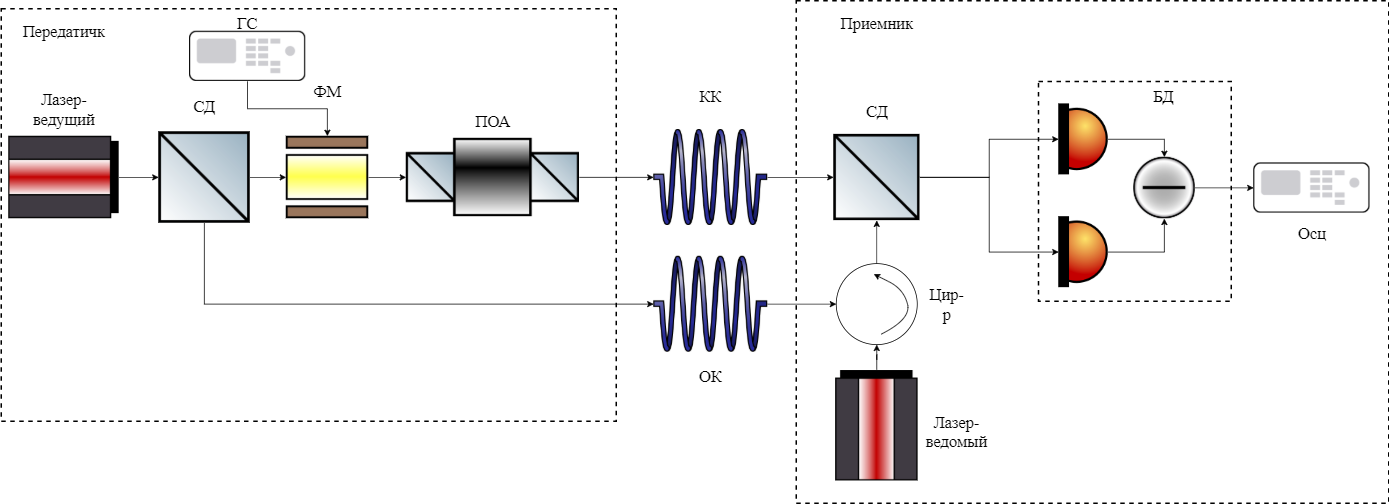
\includegraphics[width=\textwidth]{images/Схема с обратной связью.png}
    \caption{Схема эксперимента системы КРК с применением оптической инжекции. СД - светоделитель, ФМ - фазовый модулятор, ГС - генератор сигналов, ПОА - перестраиваемый оптический аттенюатор, КК - квантовый канал, ОК - открытый канал, Цир-р - циркулятор, БД - балансный детектор, Осц - осциллограф.}
    \label{fig:opt inj scheme}
\end{figure}
Данная система, оптическая схема которой изображена на рисунке \ref{fig:opt inj scheme}, работает следующим образом. На стороне передатчика излучение, сгенерированное лазером, разделяется на две части. Первая часть излучения попадает на фазовый модулятор Алисы, где происходит фазовая модуляция переменным электрическим сигналом, в который вносятся фазовые сдвиги для кодирования информации.В качестве кодирования может использоваться квадратурно-фазовая манипуляция или Quadrature Phase Shift Keying (QPSK) модуляция. Данный цифровой способ модуляции вносит фазовые сдвиги, соответствующие значениям 45\textdegree, 135\textdegree, 225\textdegree и 315\textdegree. Этим значениям фазовых сдвигов присваивается значение бит {00, 01, 10, 11}. В результате этого в спектре появляются три гармоники сигнала: $\omega$ - центральная частота лазера, $\omega$ - $\Omega$ - нижняя боковая частота  и $\omega$ + $\Omega$ - верхняя боковая частота, где $\Omega$ - частота модуляции. Излучение после модуляции описывается уравнением: 
\begin{align}
\label{eq:spectrum seed}
F_s(t) & = A_0 * \sin(\omega_0 t + \phi_0) + \frac{A_0 * m}{2} * (\sin((\omega_0 + \Omega)t + (\phi_0 + \phi (t))) - \notag \\
&- \frac{A_0 * m}{2} * (\sin((\omega_0 - \Omega)t + (\phi_0 - \phi (t))),
\end{align}где $A_0$ - амплитуда исходного излучения,  $\omega$ - центральная частота лазера, $\omega$ - $\Omega$ - нижняя боковая частота  и $\omega$ + $\Omega$ - верхняя боковая частота, $\Omega$ - частота модуляции, $\phi_0$ - фаза исходного излучения, $\phi(t)$ - фаза модулирующего излучения, $t$ - время, $m$ - индекс модуляции. Индекс модуляции - величина отношения мощности на боковых частотах к мощности во всем спектре. Индекс модуляции пропорционален амплитуде модулирующего электрического сигнала.  Полученный спектр попадает на переменный оптический аттенюатор, затухание которого выстраивается таким образом, чтобы на боковых частотах была мощность соответствующая заданному среднему числу фотонов, когда несущая может оставаться классической. Подготовленные квантовые состояния передаются в квантовый канал. 
Вторая же часть излучения проходит по отдельному волоконно-оптическому каналу на сторону приемника, где попадает в волоконно-оптический циркулятор так, что излучение заходит в резонатор ведомого лазера. 
Пришедшее излучение из квантового канала попадает на первый вход волоконного светоделителя с двумя входами и двумя выходами и коэффициентом деления 50:50. На второй же вход светоделителя попадает локальный осциллятор, представляющий собой излучение, сгенерированное отдельным лазером на приемной стороне. Благодаря наличию обратной связи в виде оптической инжекции, длина волны лазера на приемной стороне синхронизирована с длиной волны лазера Алисы. В результате ЛО и квантовые состояния интерферируют на светоделителе. В результате этой интерференции на выходе светоделителя появляются дополнительные гармоники на промежуточной частоте. Эти гармоники -  $\omega$ - $f$ - центральная частота лазера Алисы минус частота ЛО, ($\omega$ - $\Omega$) - $f$  - нижняя боковая частота минус частота ЛО   и ($\omega$ + $\Omega$) - $f$ - верхняя боковая частота минус частота ЛО, где $\Omega$ - частота модуляции, $\omega$ - частота лазера Алисы, $f$ - частота ЛО. 
\newlineРезультат этой интерференции регистрируется балансным детектором. Это устройство представляет собой два классических фотодиода, подключенных так, чтобы их токи вычитались. Такое подключение позволяет уменьшить собственные шумы детектора. После этого полученный ток попадает на фильтр низких частот для фильтрации постоянной составляющей. Полученный сигнал усиливается каскадом усилителей и передается на АЦП.  В результате на выходе балансного детектора формируется только один сигнал на частоте, совпадающей с частотой модуляции на стороне передатичка. Происходит это по той причине, что длина волны ЛО и лазера передатчика совпадают благодаря обратной связи в виде оптической инжекции. Таким образом на выходе детектора остается только составляющая ($\omega$ + $\Omega$) - $f$, а остальные преобразуются в постоянную составляющую, которые фильтруются. 
\begin{figure}
    \centering
    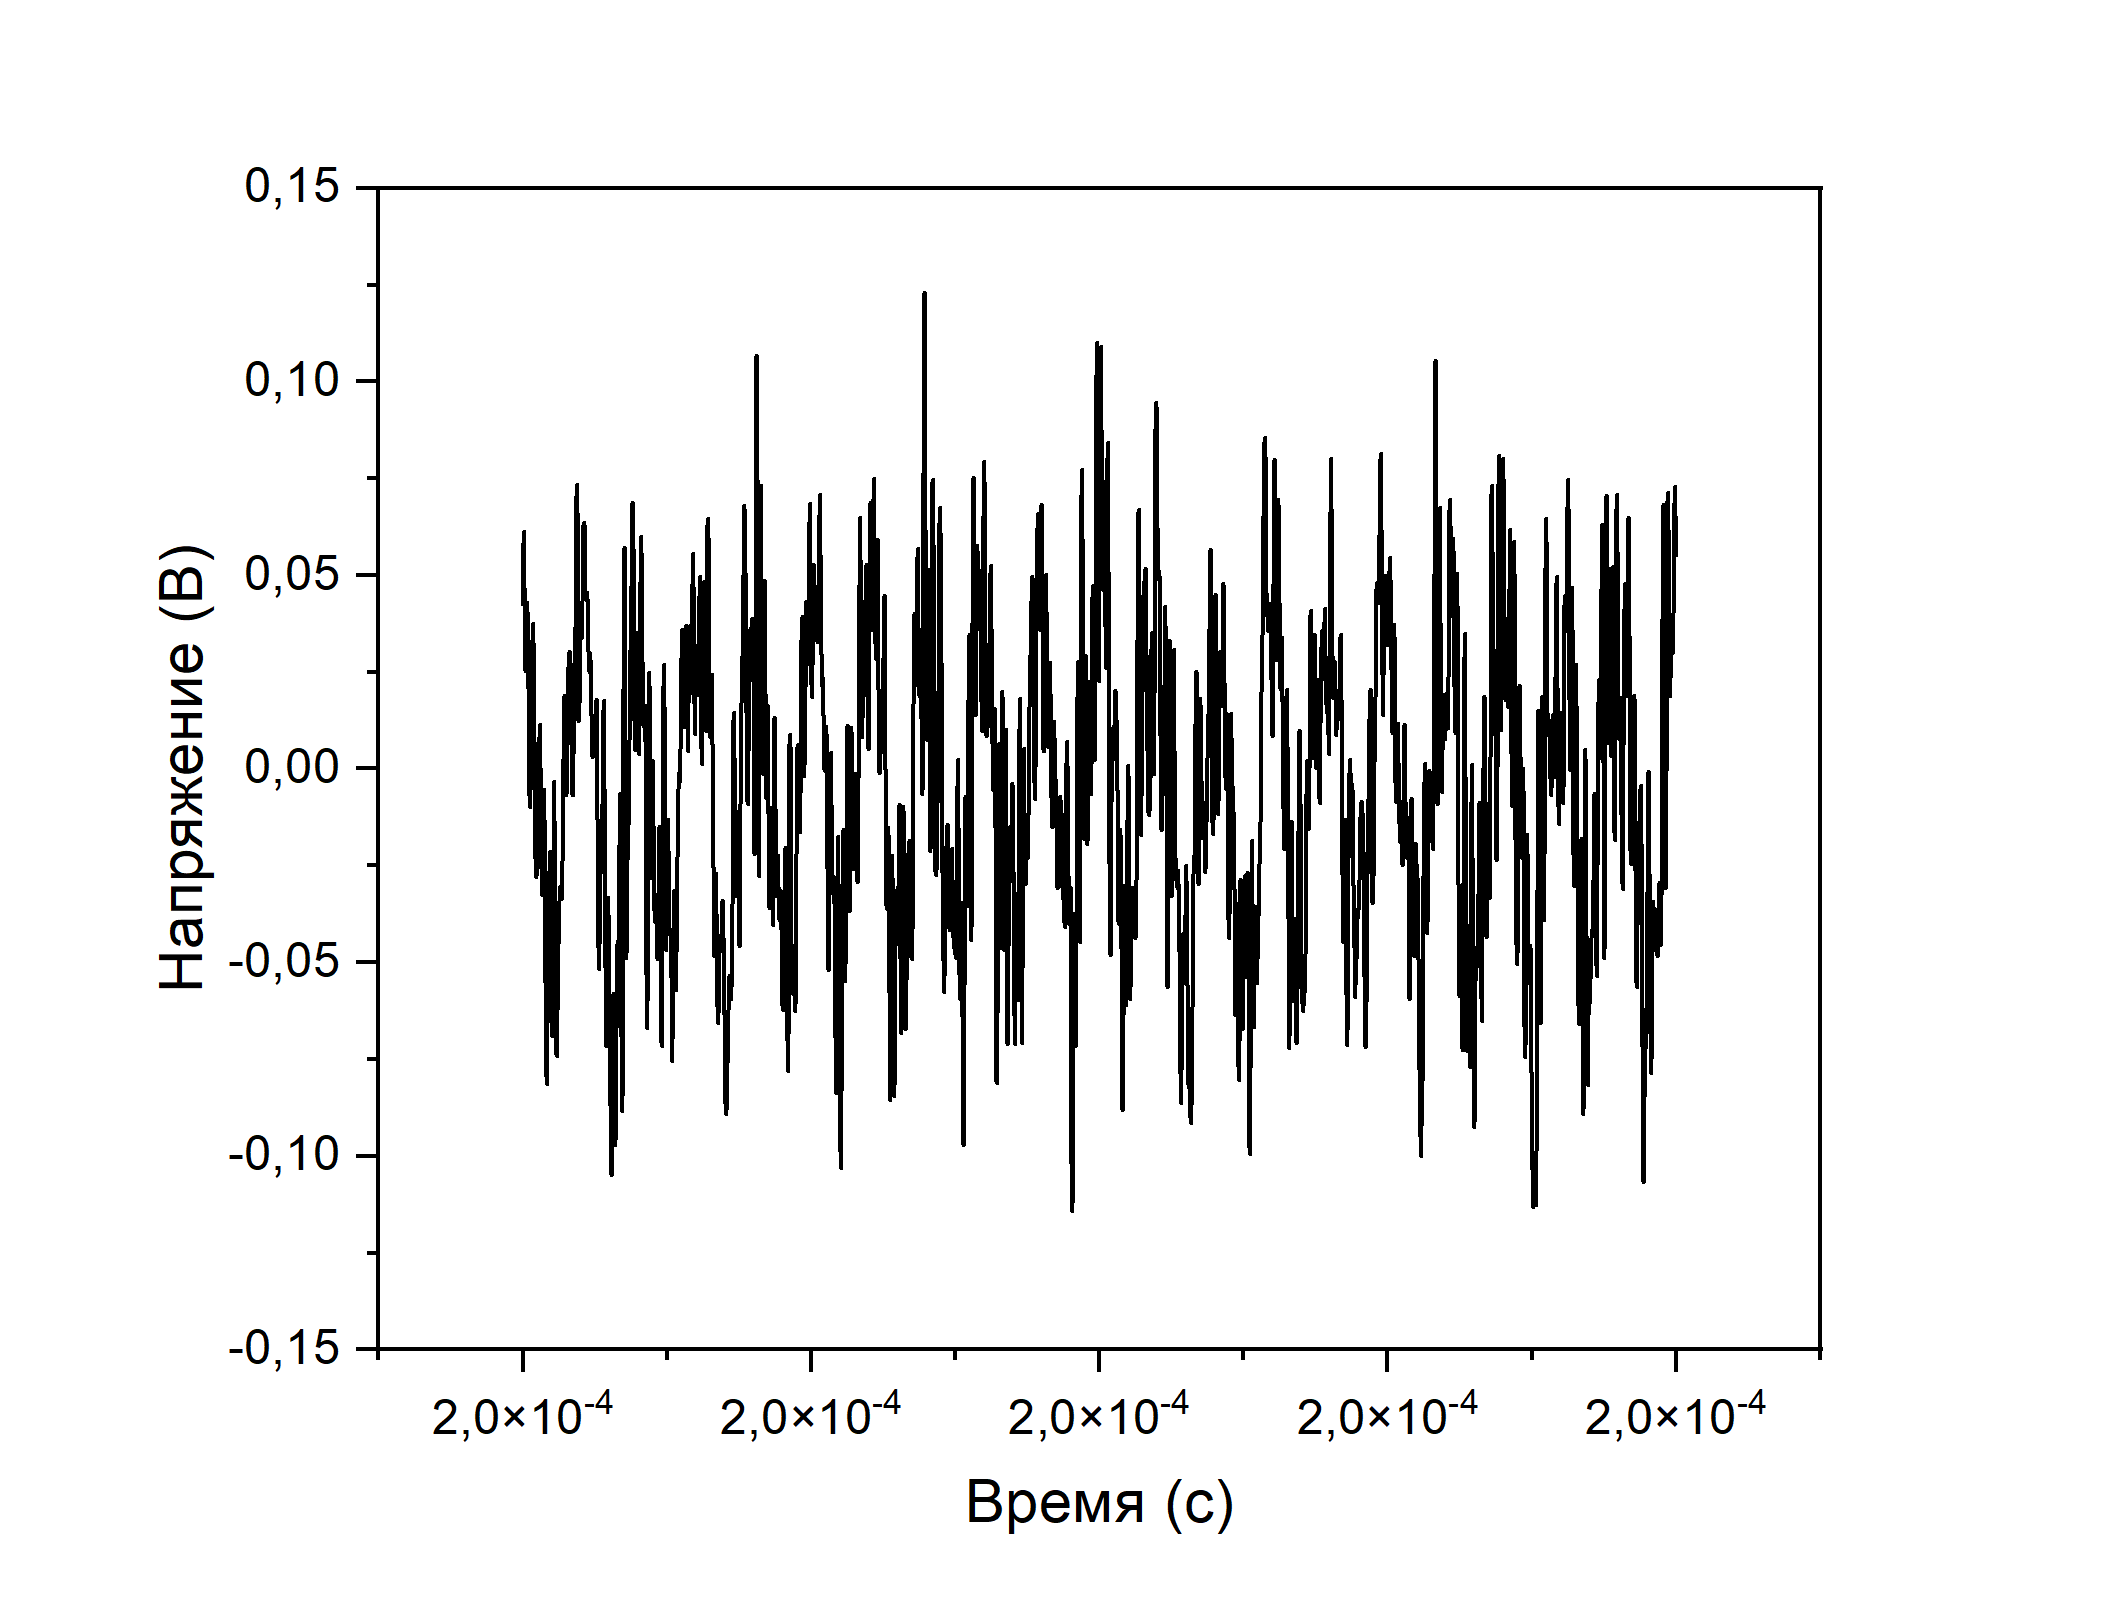
\includegraphics[width=\textwidth]{images/03.png}
    \caption{Зашумленный сигнал на выходе балансного детектора}
    \label{fig:noisy output inject}
\end{figure}
Полученное колебание на выходе балансного детектора несет в себе информацию о фазе, закодированную Алисой. Данный сигнал обрабатывается цифровыми методами обработки сигналов для извлечения значения фаз сигнала. 
\begin{figure}
    \centering
    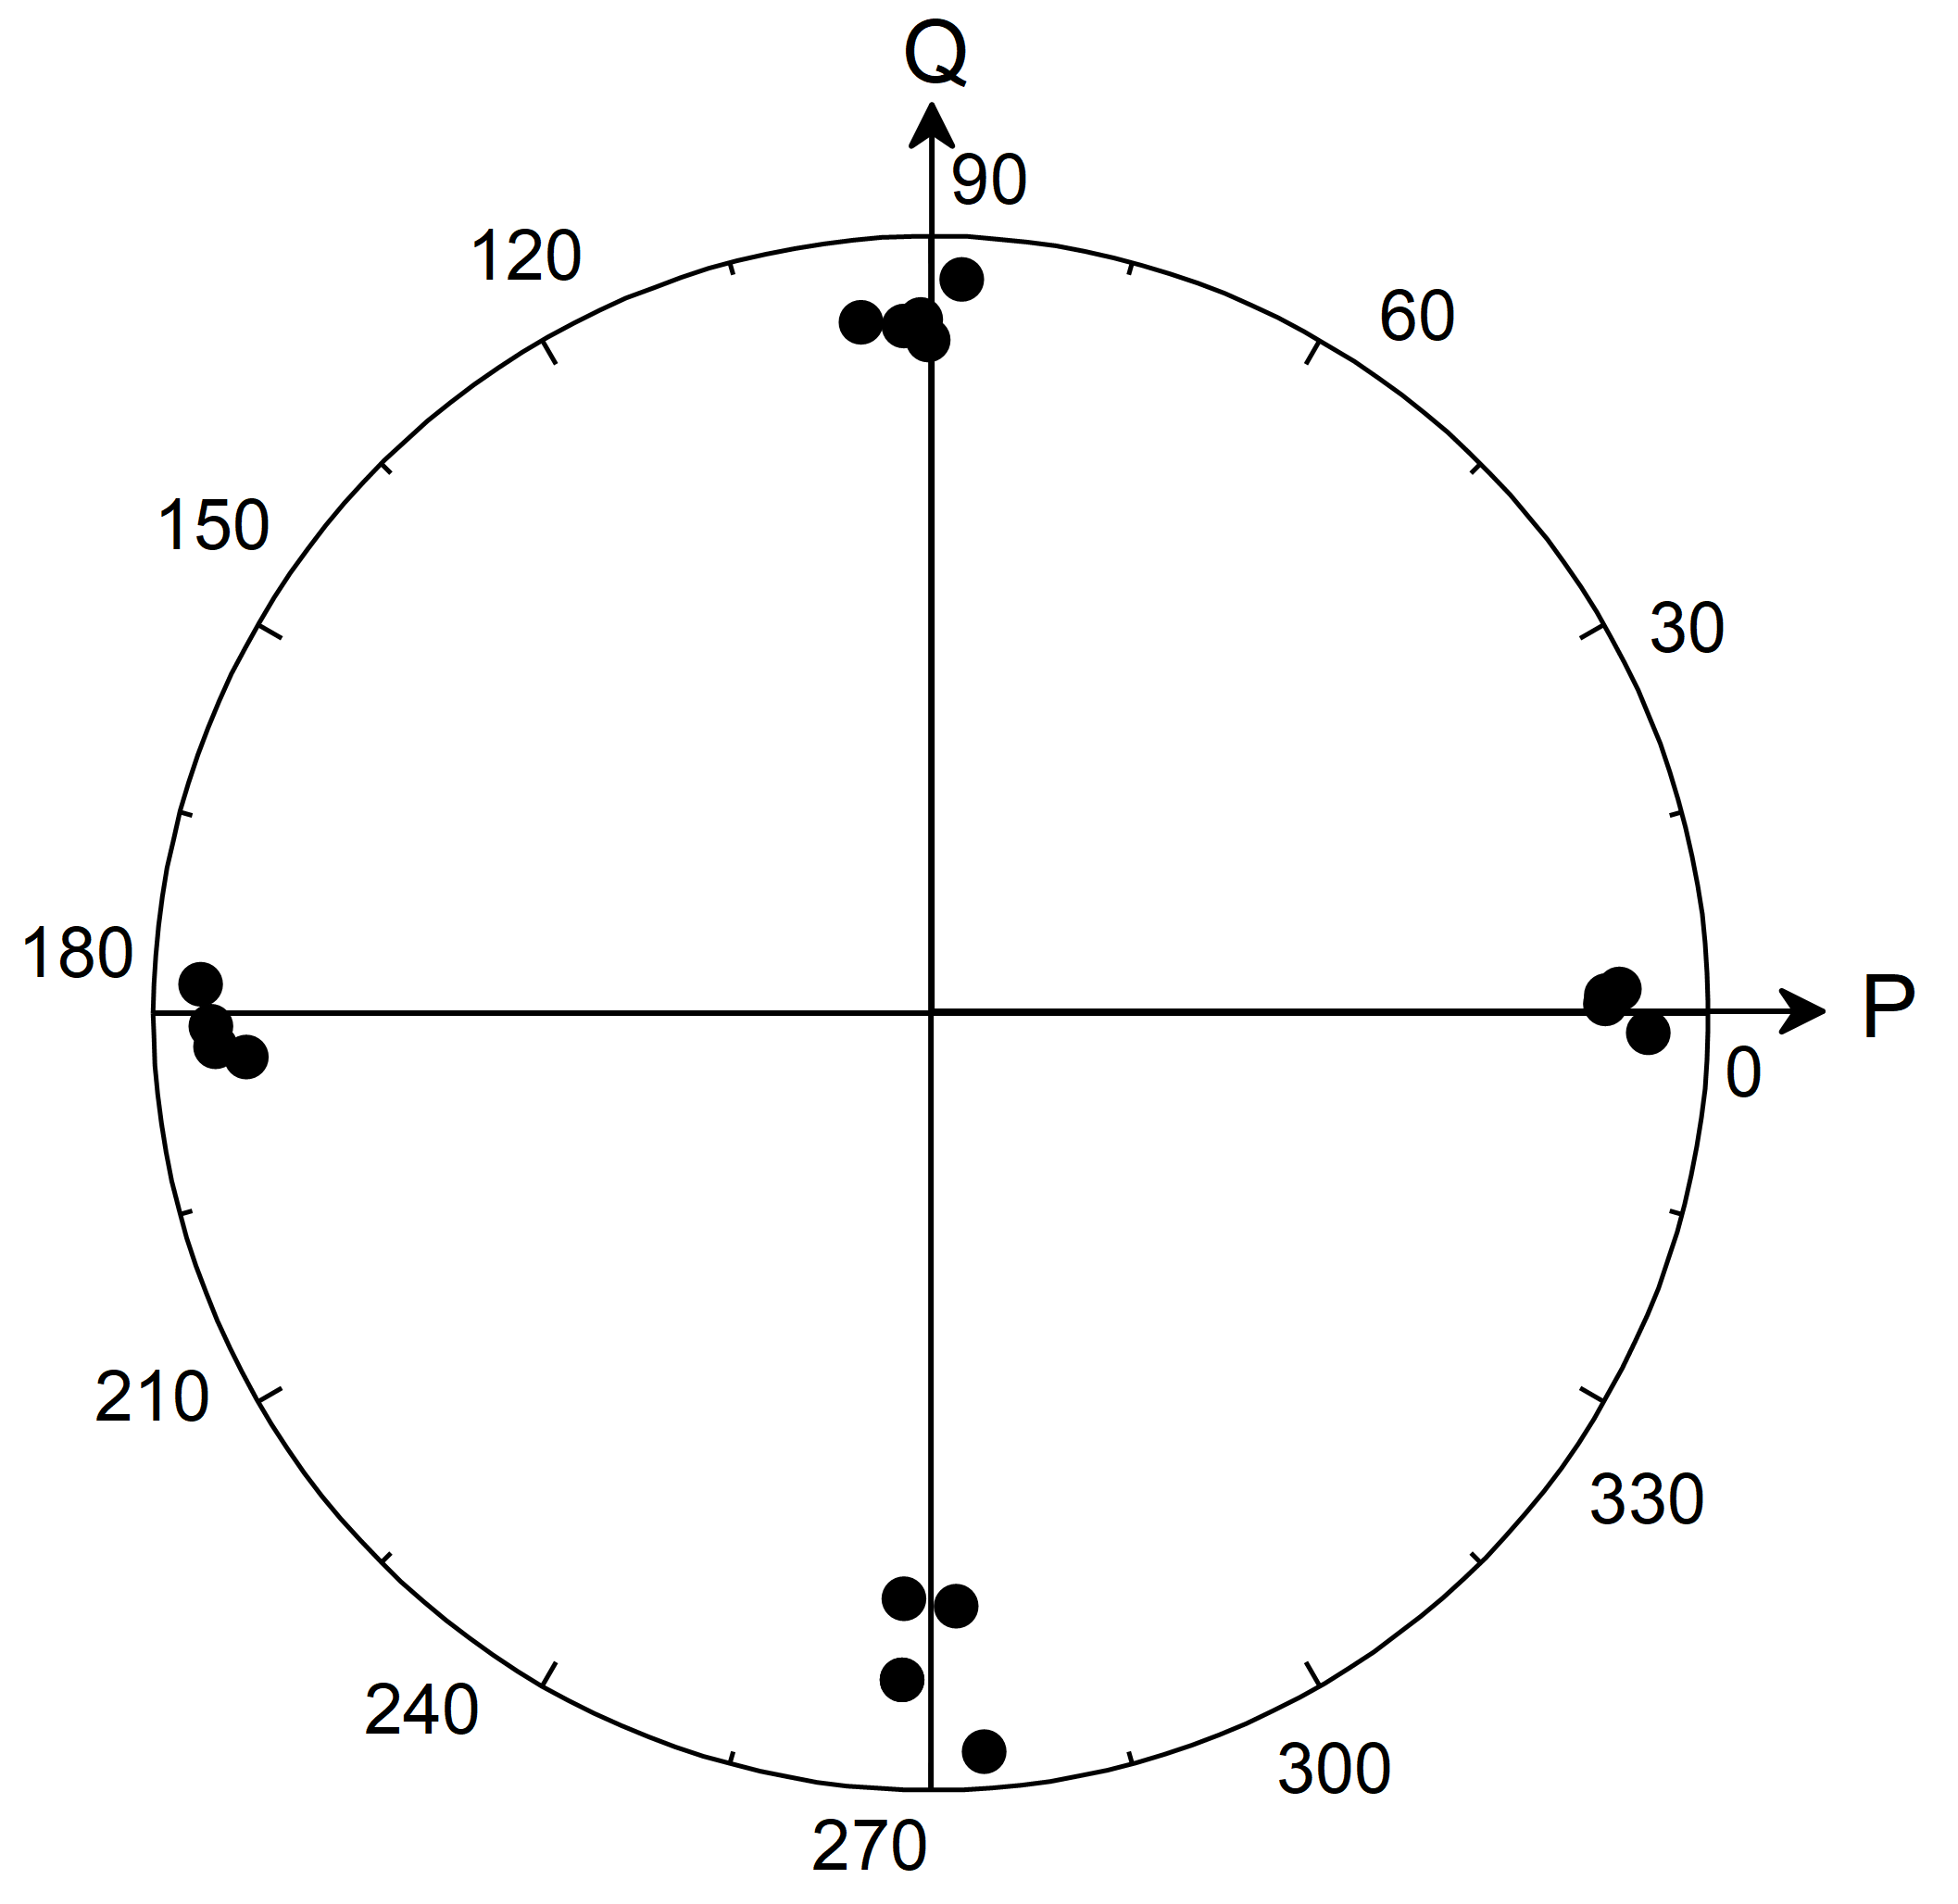
\includegraphics[width=0.8\textwidth]{images/06.png}
    \caption{Полученные значения фазы после цифровой обработки}
    \label{fig:phase meas ijnect}
\end{figure}

Полученная последовательность бит является сырым ключом. Полученный ключ просеивается. В полученном просеянном ключе оценивается квантовый коэффициент ошибок по битам или QBER, предварительно открыв часть ключа. И последним этапом происходит усиление секретности  с помощью HASH-функций.
\newline К плюсам данного метода реализации КРК можно отнести простоту системы, благодаря тому, что отстуствует активный выбор базиса в виде модулятора любого типа. Наличие обратной связи в виде оптической инжекции позволяет решить несколько проблем: стабилизация длины волны ЛО, что так же упрощает конечную систему, и уменьшает фазовые шумы, связанные со случайностью фазы лазерного излучения, сгенерированного разными источниками. Применение же гетеродинного метода приема позволяет использовать любой тип модуляции, что позволяет гибко настраивать протокол под различные задачи и оставляет задел на будущее для увеличения скорости выработки ключей.
\newline К недостаткам данной системы можно отнести необходимость дополнительного волоконно-оптического канала связи для организации обратной связи, что частично нивелируется тем, что реальные системы КРК встраиваются в уже существующие системы передачи данных, которые работают с технологией мультплексирования и сигнал оптической инжекции можно встроить в уже применяемые каналы, так как у него нет требований к уровню сторонних шумов. Второй же недостаток - это уязвимость к атаке засева лазера, который требует дополнительного изучения и контрмер. 
\newpage В \underline{третьей главе} рассматривается схема применения гетеродинного метода детектирования сигналов с двумя независимымми источниками сигналов для протокола квантовой коммуникации на боковых частотах. Особенностью данной системы является перенос квантовых состояний света на боковые частоты, которые появляются в спектре излучения. Основная реализация данного протокола предполагает использование дискретных переменных и детекторов одиночных фотонов на основе лавинных фотодиодов для регистрации сигналов. Однако этот протокол возможно адаптировать и для использования когерентных методов детектирования. 
\newline В данной работе предлагается использование гетеродинного метода детектирования сигналов для системы квантовой коммуникации на боковых частотах.
\begin{figure}
    \centering
    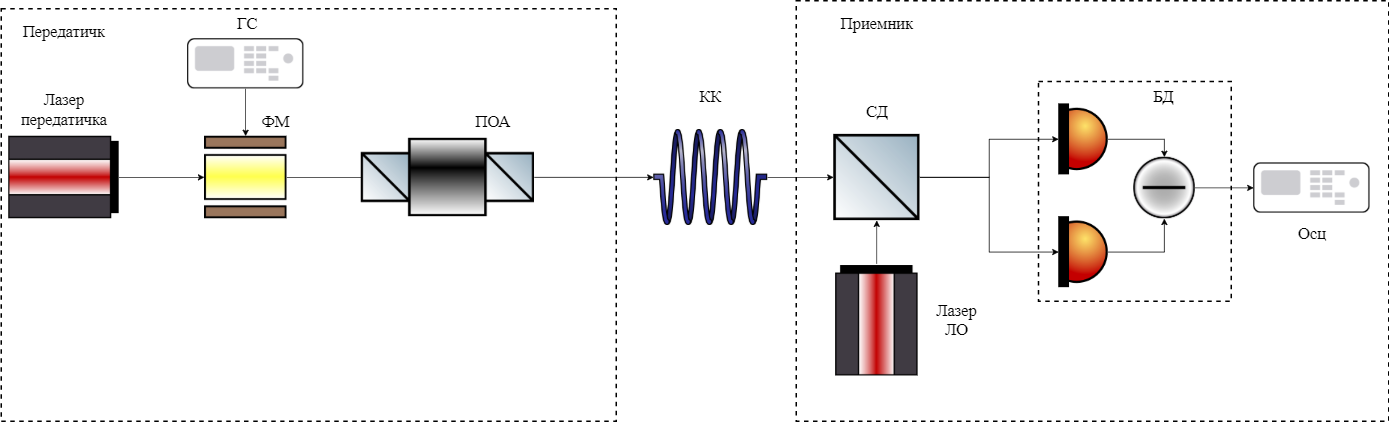
\includegraphics[width=\textwidth]{images/Гетеродин схема.png}
    \caption{Схема системы квантового распределения ключа на боковых частотах с независимым локальным осциллятором. СД - светоделитель, ФМ - фазовый модулятор, ГС - генератор сигналов, ПОА - перестраиваемый оптический аттенюатор, КК - квантовый канал, БД - балансный детектор, Осц - осциллограф.}
    \label{fig:het true scheme}
\end{figure}
Данная система работает следующим образом. Лазер на передающей стороне форимрует когерентное излучение. Это излучение, пройдя необходимые пассивные элементы в виде оптических изоляторов, попадает на  кристалл фазового модулятора. На электрический же вход фазового модулятора передается переменное напряжение на частоте модуляции. В это напряжение вносится фазовый свдиг, который соответсвует битам информации. Для примера в данной работе используется квадраратурно-фазовая манипуляция или quadrature phase-shift keying (QPSK). Значения фазовых сдвигов в таком случае это {45\textdegree, 135\textdegree, 225\textdegree и 315\textdegree} и этим фазовым сдвигам соответствуют следующие биты информации {00, 01, 10, 11}. В результате такой модуляции в спектре излучения после фазового модулятора появляются три гармоники, в двух из которых закодирована информация от передатичка. Подготовленное излучение ослабляется переменным аттенюатором для достижения уровня мощности на боковых частотах меньше 1 фотона в среднем. Полученные таким образом квантовые состояния передаются по волоконно-оптической линии связи на приемную сторону.  
\newline Переданный сигнал от Алисы после прохождения ВОЛС попадает на контроллер поляризации для компенсации искажений, внесенных прохождением через волокно. После этого установленный поляризационный светоделитель выделяет лишь нужную поляризацию и пропускает излучение с нужной поляризацией дальше. После этого квантовые состояния смешиваются с ЛО, сгенерированным отдельным лазером, на светоделителе с двумя входами и двумя выходами и коэффициентом деления 50:50. Эти сигналы интерферируют и в результате этой интерференции спектр излучения обогощается дополнительными гармониками. Эти гармоники появляются из-за того, что частоты ЛО и лазера Алисы не совпадают. Появишвиеся гармоники находятся на различных частотах - суммарная, разностная и комбинационные. Но с учетом ограниченности полосы пропускания балансного детектора, мы можем наблюдать на его выходе только гармоники на разностных частотах, которые в нее попадают. Суммарные и другие комбинационные частоты не попадают в полосу пропускания БД и регистрируются как постоянная составляющая, которая теряет всю информацию, закодированную в их фазы. Когда как гармонические колебания на разностной промежуточной частоте проходят усилительный каскад без изменений и сохраняют информацию, закодированную в фазу излучения Алисой. Таким образом происходит перенос спектра из оптической области в радиочастотную, где упрощается усиление и обработка сигналов. 
\begin{figure}
    \centering
    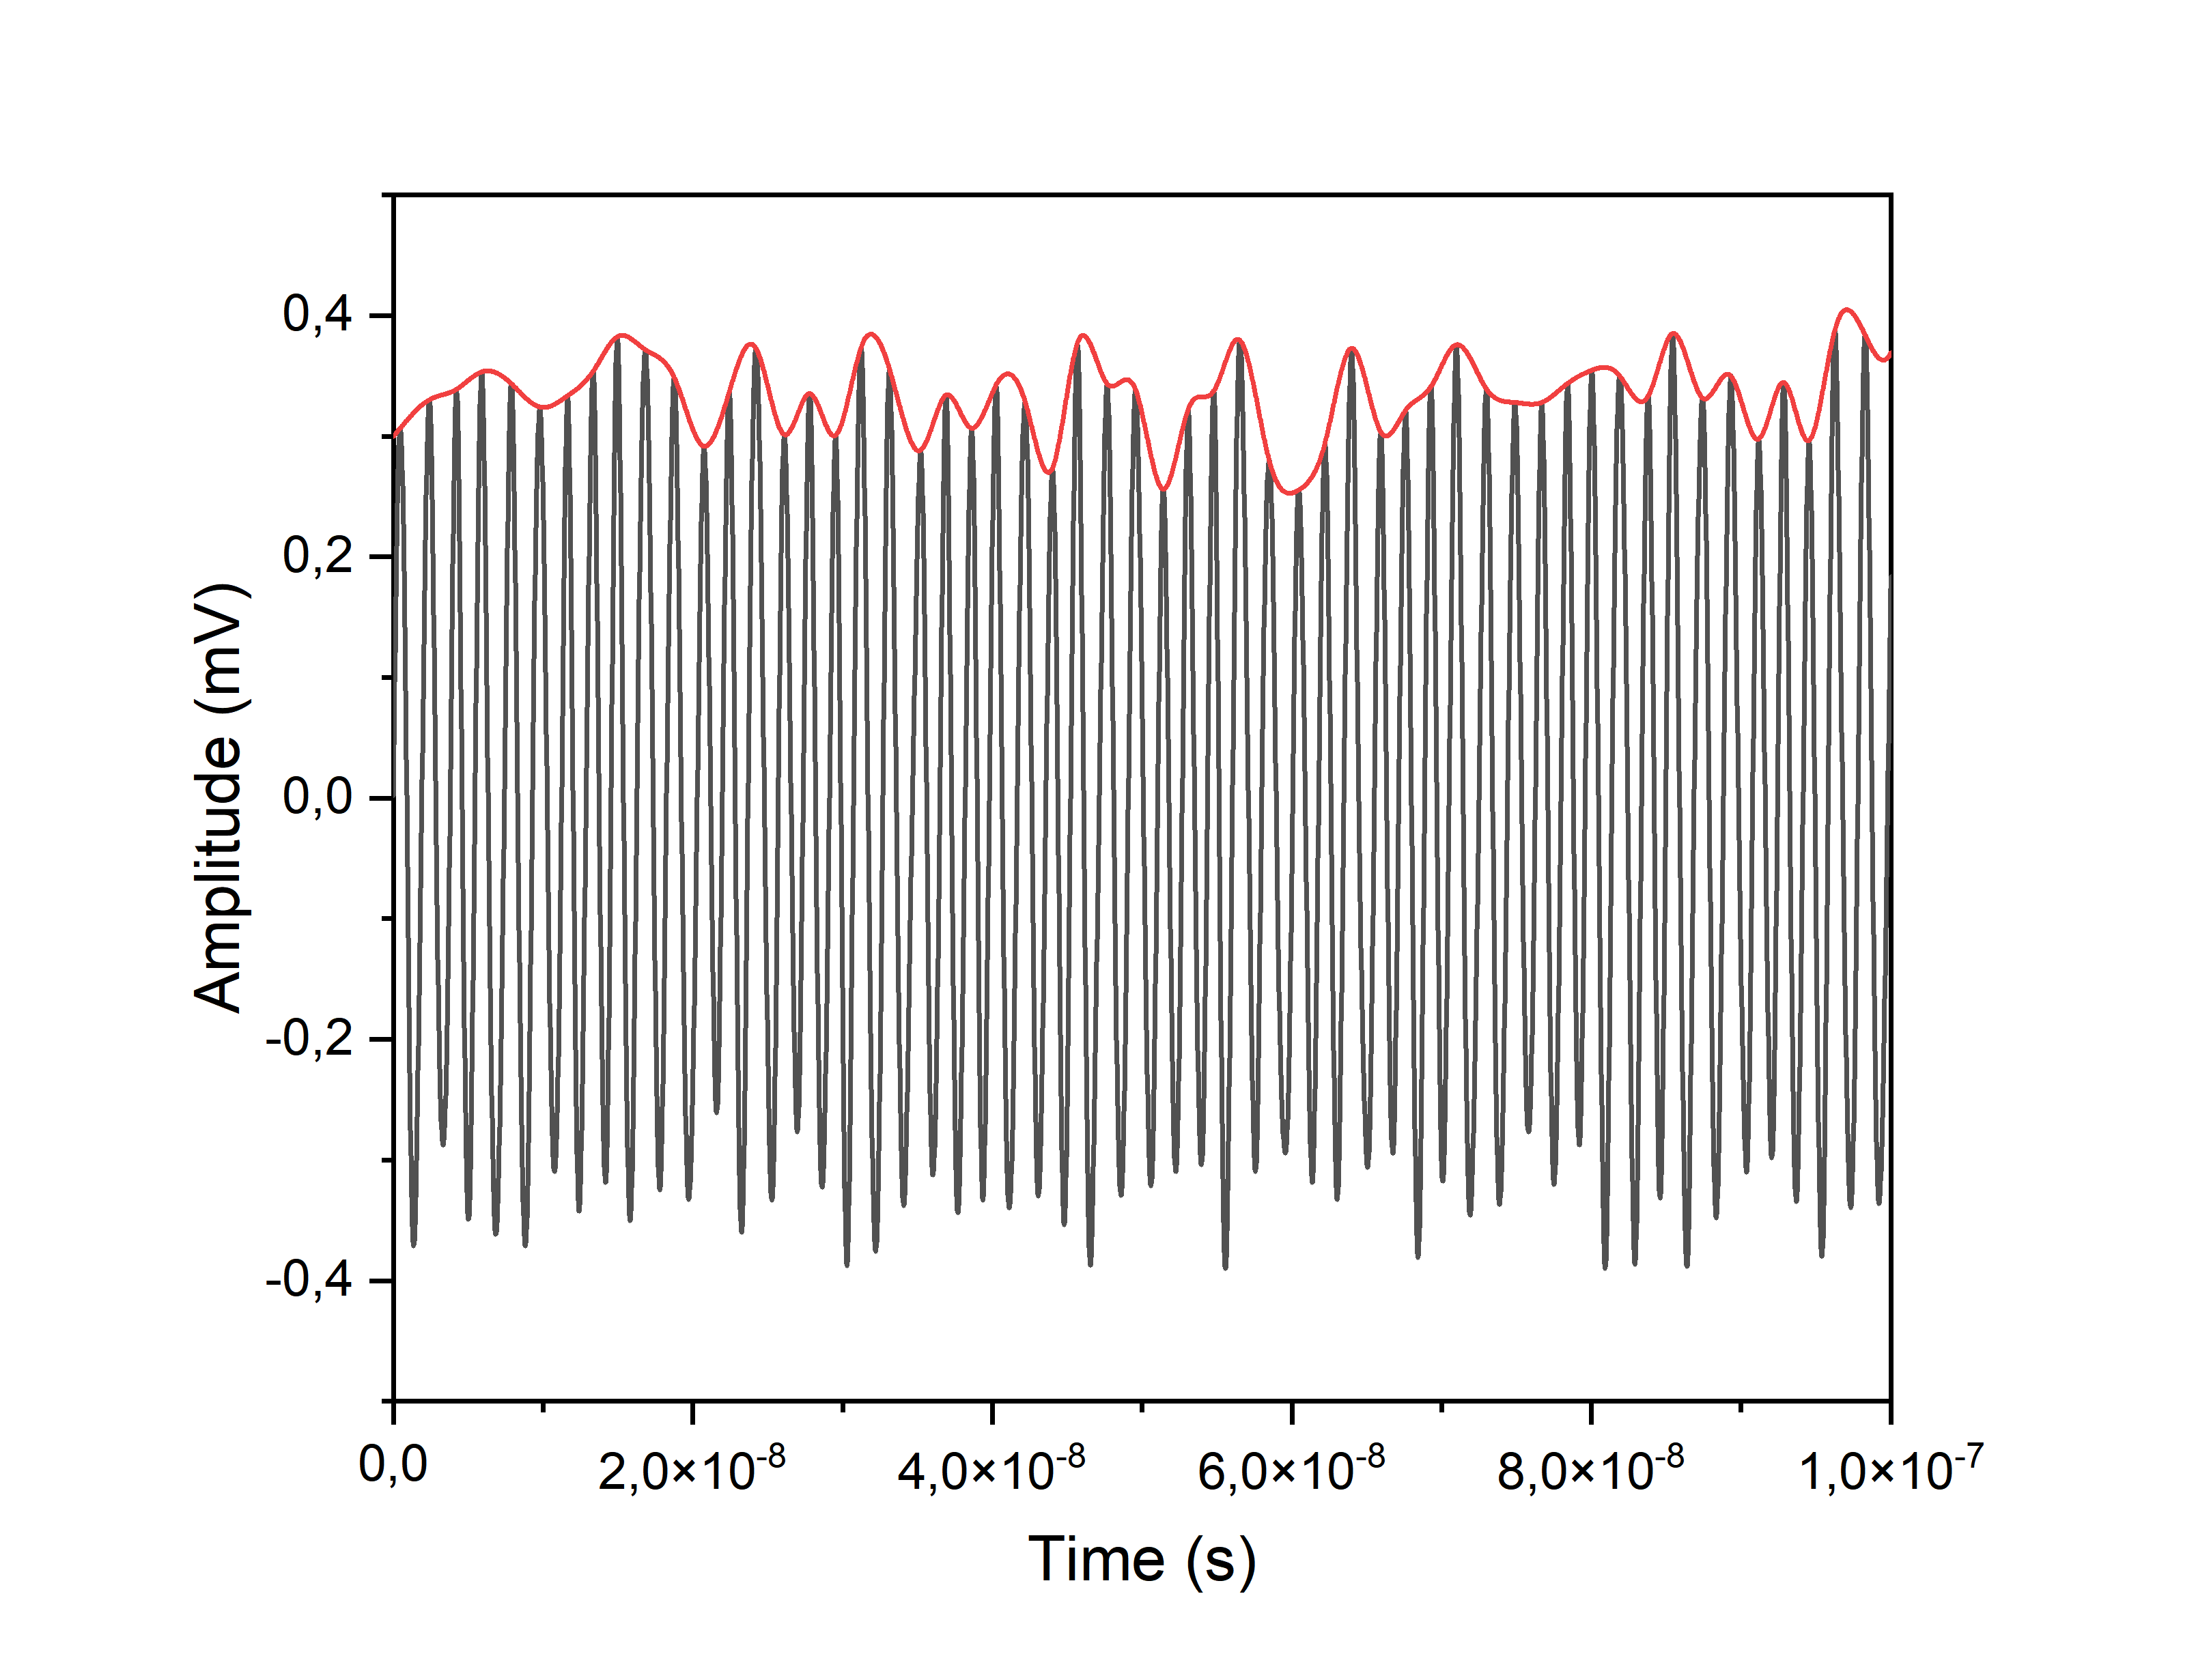
\includegraphics[width=\textwidth]{images/balanced output heterodyne.png}
    \caption{Сигнал на выходе балансного детектора после гетеродинного приема.}
    \label{fig:het time output}
\end{figure}
\newline Балансный детектор - это устройство, которое  представляет собой два фотоприемных диода, подключенных так, чтобы их фототоки взаимно вычитались. После этого полученный сигнал подвергается фильтрации, чтобы исключить влияние постоянной составляющей фототока. После этого полученный сигнал попадает на каскад усилителей для увеличение его амплитуды. Наличие каскада усилителей ограничивает полосу пропускания всего устройства. Типичная ширина полосы пропускания может варьироваться от 100 МГц до 1.2 ГГц. Это ограничивает диапазон принимаемых частот и скорость выработки сырого ключа. 
\newline Полученный сигнал после усиления необходимо перевести в цифровую форму с помощью АЦП для его дальнейшей обработки. В качестве обработки могут применятся различные методы цифровой обработки сигналов, такие как Быстрое Преобразование Фурье или Преобразование Гильберта. В результате этой обработки из гармонического сигнала, полученного после АЦП, генерируются фазовые значения, которым соответствуют заданные значения бит, из которых формируется битовая последовательность, называемая сырым ключом. 
\newline К достоинствам данного метода можно отнести гибкость выбора протокола, так как перенос информации на промежуточную частоту позволяет анализировать практически любую модуляцию без необходимости внесения дополнительных элементов, например, фазового модулятора для выбора базиса. Использование двух независимых источников когерентного излучения позволяет не использовать системы обратной связи, которые требуют дополнительного оптического канала и открывают дополнительные возможности для злоумышленника. Генерация локального осциллятора на стороне приемника позвволяет увеличить его мощность, по сравнению с протоколами, в которых ЛО передается по квантовому каналу, что позволяет уменьшить шумы, связанные с рассеянием в ВОЛС и увеличить соотношение сигнал/шум, что положительно влияет на скорость выработки бит. 
\newline Из недостатков же можно выделить необходимость подстройки частоты, так как два независимых генератора нуждаются в периодической подстройке частоты. Эта проблема решается особенностью протокола квантовой коммуникации на боковых частотах за счет того, что в спектре присутствует мощная несущая, которая так же сбивается с локальным осциллятором и переносится на промежуточную частоту. Анализируя эту частоту после обработки БПФ, можно подстраивать частоту ЛО для того, чтобы все сигналы попадали в полосу пропускания балансного детектора. Другим же недостатком является случайный фазовый шум из-за случайности процесса генерации лазерного излучения в двух независимых источниках. Данная проблема решается анализом фазы промежуточной частоты между локальным осциллятором и оптической несущей, полученной после фазовой модуляции Алисы. Этот сигнал будет содержать фазовый шум и ЛО, и лазера передатчика, который можно учесть в постобработке, сделав предварительную обработку цифровыми методами. 
\newpage \underline{Четвертая глава} посвещена изучению влияния излучения злоумышленника на длине волны 1310 нм на источник когерентного излучения на основе полупроводникового лазерного диода с распределенной обратной связью. Данная уязвимость в технической реализации получила название атака оптической накачкой. Данный тип атаки схож с атакой оптическим "засевом" (Laser Seeding) тем, что Ева инжектирует свое излучение в резонатор лазера на передатичке для изменений его характеристик. Однако есть существенное различие. В случае атаки "засевом" злоумышленник использует ту же или близкую длину волны к рабочей длине волны атакуемого лазера. В то время как в случае атаки оптической накачкой Ева использует длину волны лазера, отличающуюся на 50 и более нанометров от рабочей длины волны лазера Алисы. Эта особенность позволяет эффективнее обходить контрмеры с применением пассивных волоконно-оптических элементов в виде изоляторов. Их коэффициент изоляции имеет спектральную зависимость, что приводит к тому, что вносимая изоляция на длине волны 1310 нм существенно меньше, чем на длине волны 1550 нм. В результате злоумышленнику требуются меньшая зондирующая мощность, чтобы достичь необходимого эффекта. 
\newline Данная атака строится следующим образом. Злоумышленник устанавливает в разрыв волоконно-оптической линии связи волоконный циркулятор с тремя портами. В первый порт подлючается зондирующий лазер Евы. Второй порт подключается в волоконно-оптическую линию связи в сторону отправителя, а третий порт - в сторону приемника. Таким образом излучение злоумышленника будет заходить в оптическую схему передатчика, а излучение Алисы будет проходить по волокну в сторону приемника без проблем. Излучение злоумышленника, проходя оптическую схему передатичка, претерпевает затухание, поэтому необходимо иметь достаточную мощность зондирующего излучения для внесения изменений в характеристики лазера. Прошедшее излучение попадает в кристалл лазера и поглощается в нем.
\begin{figure}
    \centering
    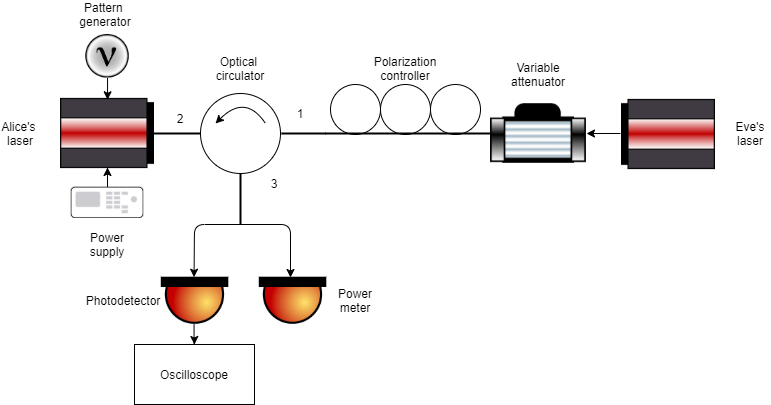
\includegraphics[width=0.75\textwidth]{images/1310 experiment.png}
    \caption{Схема эксперимента по засеиванию лазера. Alice's Laser -  Лазер Алисы, Pattern generator - генератор последовательности импульсов, Power Supply - лабораторный блок питания, optical circulator - оптический циркулятор, polarization controller - контроллер поляризации, varriable attenuator - перестраиваемый аттенюатор, Eve's laser - лазер злоумышленника, Photodetector - фотоприемник, power meter - измеритель мощности, Oscilloscope - осциллограф.}
    \label{fig:exper 1310 ref}
\end{figure}
Это приводит к тому, что создается дополнительная инверсия населенности, приводящая к смещению Ватт-Амперной характеристики лазера при неизменном токе накачки.
\begin{figure}
    \centering
    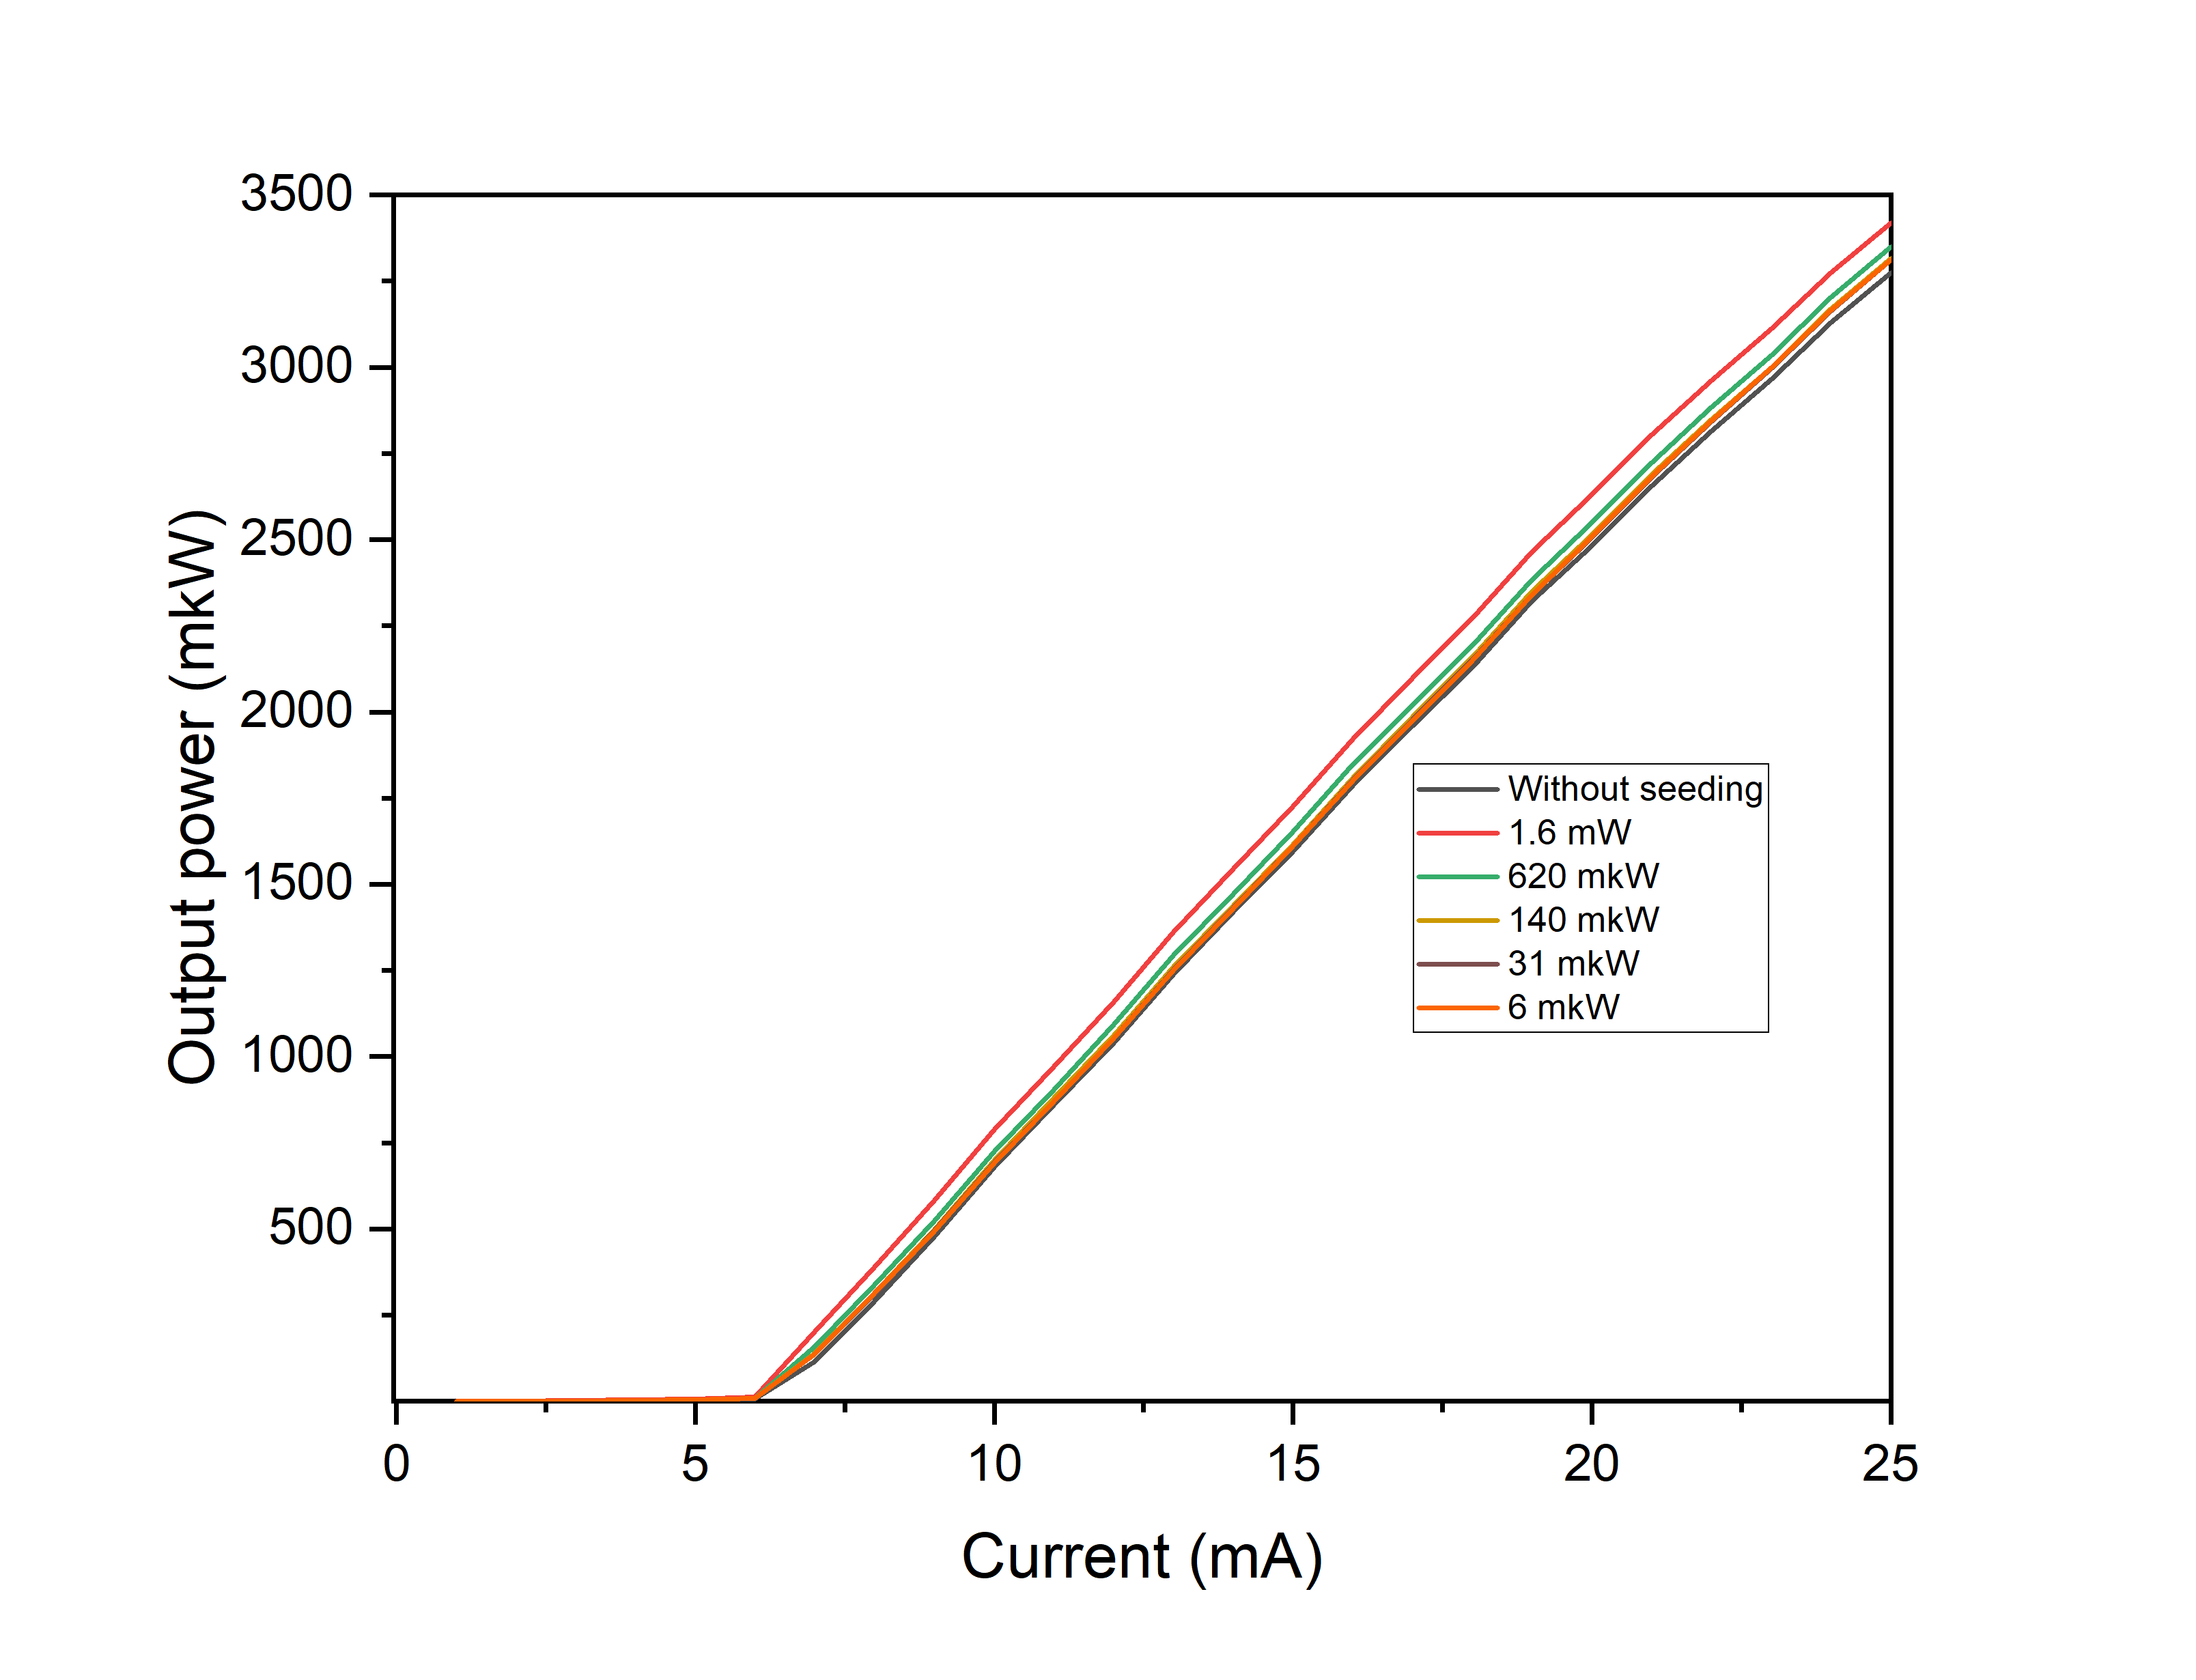
\includegraphics[width=0.75\textwidth]{images/ватт ампер для диссера.png}
    \caption{Изменение Ватт-Амперных характеристик под различными мощностями накачки на длине волны 1310 нм. Output power - выходная мощность в микроваттах, current - ток в миллиамперах}
    \label{fig:watt-amp ref}
\end{figure}
В результате этого калиброванный источник излучения на стороне передатичка начинает излучать большую мощность, чем предполагалось изначально. В итоге это приводит к тому, что выходное среднее число фотонов увеличивается, генерируется большее количество многофотонных состояний, что открывает возможности по реализации атаки с ращиплением числа фотонов. Этот же эффект проявляется в изменении формы импульса. Оптическая накачка увеличивает площадь импульса и, соответсвенно, его энергию. Отдельно стоит отметить, что в случае оптической накачки, генерация импульса начинается раньше, чем при обычном режиме работы лазера передатичка, что злоумышленник так же может использовать для различения состояний ловушек и квантовых состояний в протоколах с использованием состояний ловушек. 
\begin{figure}
    \centering
    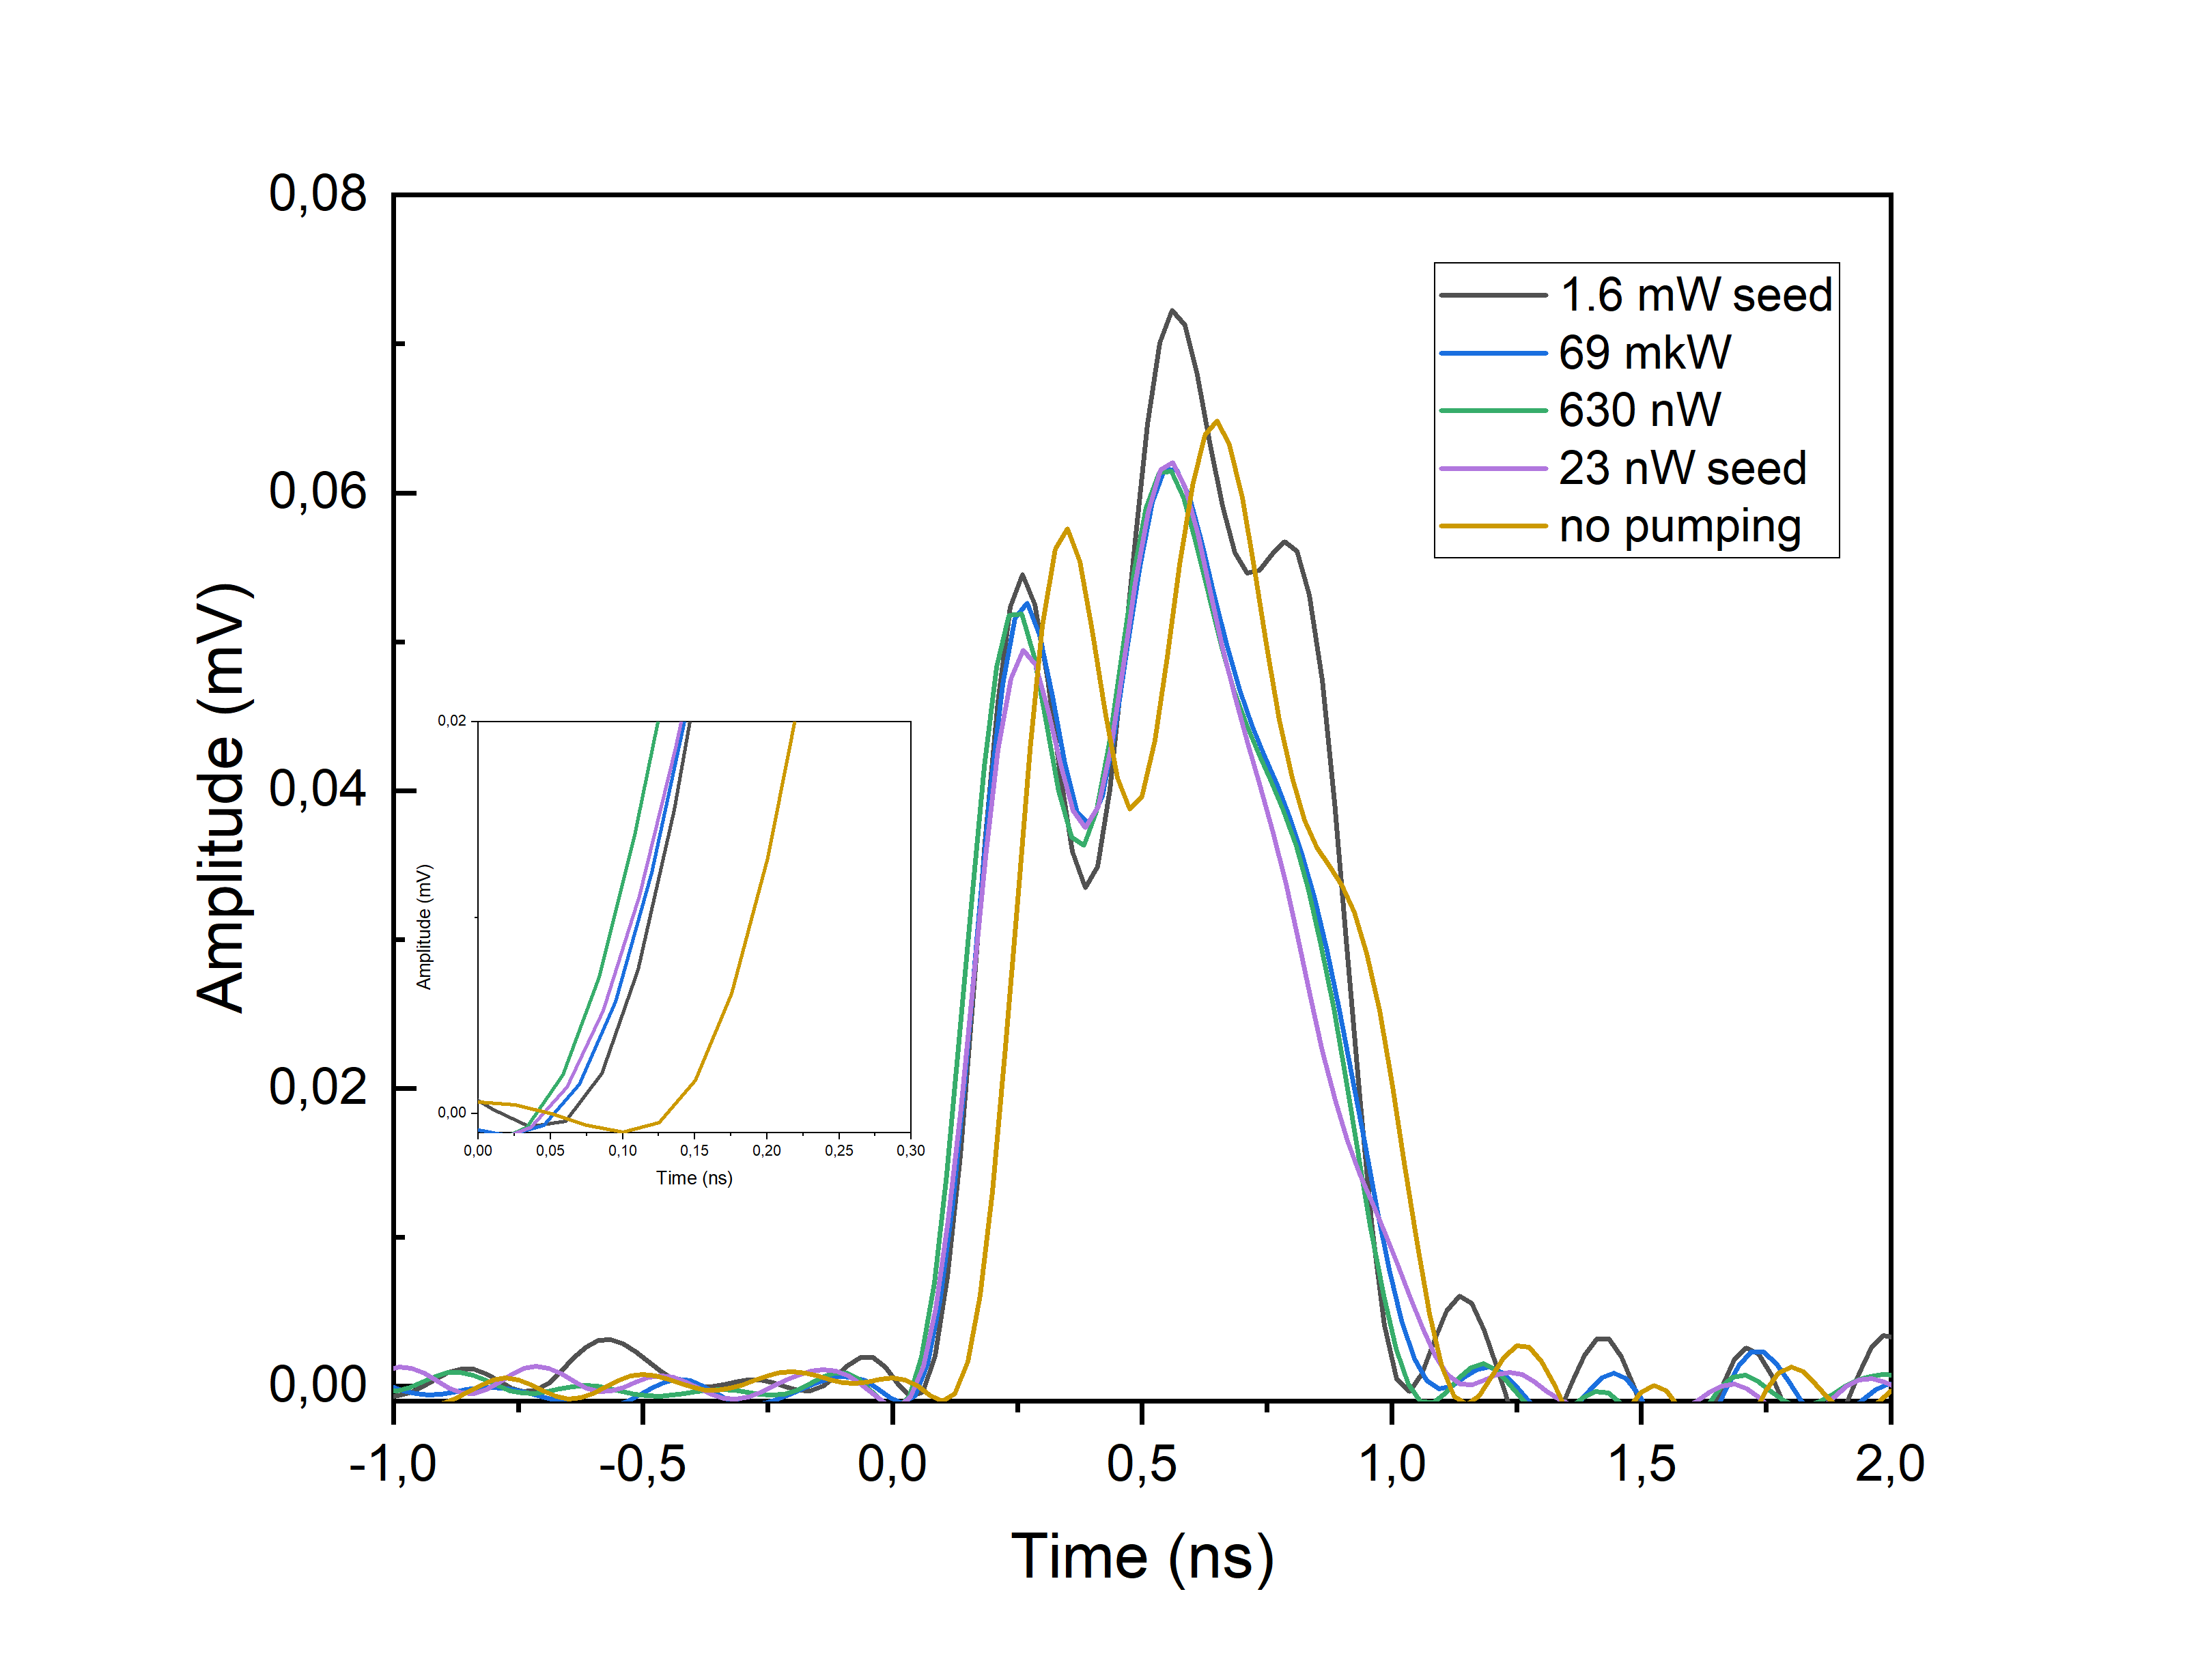
\includegraphics[width=0.75\textwidth]{images/Импульсы под действием 1310 для диссера.png}
    \caption{Измнение формы импульса под действием внешней оптической накачки на разных мощностях на длине волны 1310 нм. Amplitude - амплитуда в милливольтах, Time - время в наносекундах, seed - засеивание, pumping - накачка.}
    \label{fig:pulses 1310 ref}
\end{figure}
\newpage В рамках данной работы показана реализация атаки оптической накачкой на длине волны 1310 нм, которая приводит к увеличению выходной мощности лазера при неизменных токах накачки, увеличению площади импульса и повышению квантовой эффективности лазера. Данные эффекты создают условия для проведения других типов атак на систему КРК. В случае данной работы было показано, что зондирующей мощности в 200 мкВт достаточно для повышения квантовой эффективнсти на 1\%, продемонстрированно на графике \ref{fig:eff ref} и увеличения выходной мощности на 4\%. Была рассчитана минимально необходимая мощность для эффективной атаки злоумышленника на типичную оптическую схему передатичка, реализующую протокол BB84.
\begin{figure}
    \centering
    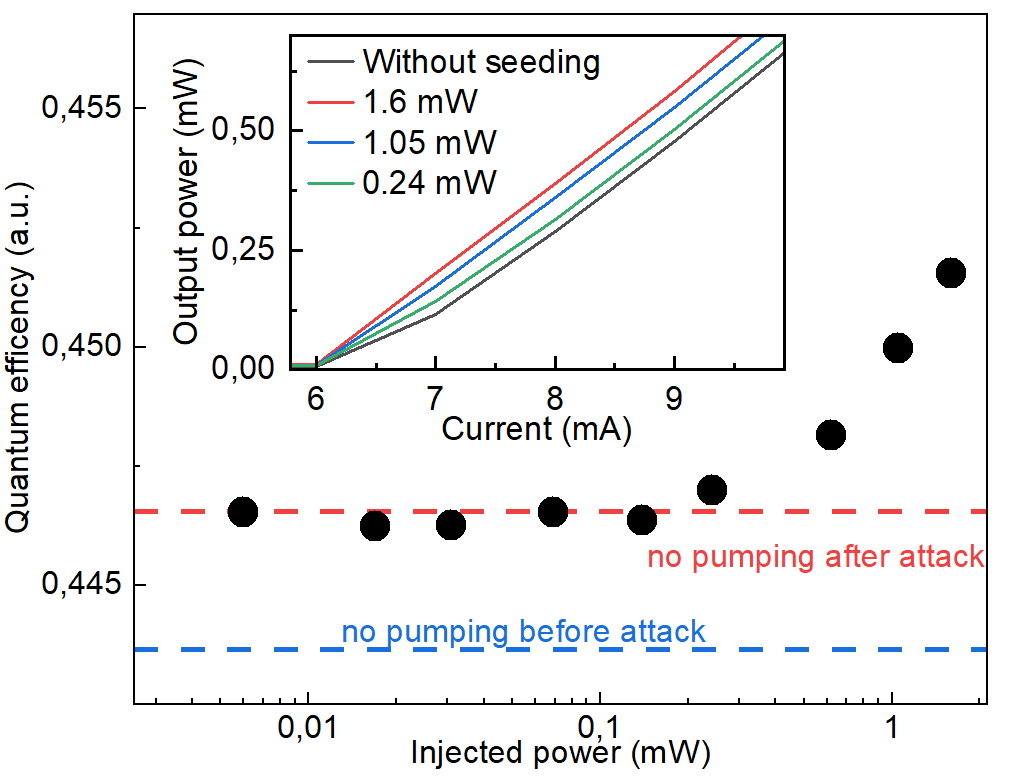
\includegraphics[width=0.7\textwidth]{images/Эффективность 1310.png}
    \caption{Изменение квантовой эффективности под действием внешнего излучения на длине волны 1310 нм. Quantum efficiency - квантовая эффективность в относительных единицах, Output power - выходная мощность в милливаттах, Injected power - введенная мощность в милливаттах, current - ток в миллиамперах, синяя  пунктирная линия - значение квантовой эффективности до атаки, красная пунктирная линия - значение квантовой эффективности после атаки. }
    \label{fig:eff ref}
\end{figure}
\newpage Исследования, проводимые в \underline{шестой главе}, посвещены изучению влияния мощного когерентного излучения на источник лазерного излучения на основе оптической инжекции. Такие источники активно используются в системах квантовой коммуникации, реализующих протокол с недоверенным приемным узлом. Такие источники обладают улучшенными характеристиками стабильности амплитуды выходного сигнала, временной стабильностью длины волны и уменьшенным чирпом выходных импульсов за счет уменьшения влияния переходных процессов во время генерации. Эти особенности позволяют получать видность интерференции Хонг-Оу-Манделя близкой к теоритическому максимуму в 0.5. 
\newline Однако, для таких источников не были исследованы методы воздейсвтия такие как атака "засевом" лазера. Для этого была собрана оптическая схема для проведения исследования влияния мощного лазерного излучения в диапазоне мощностей от 180 до 900 мВт. 
\begin{figure}
    \centering
    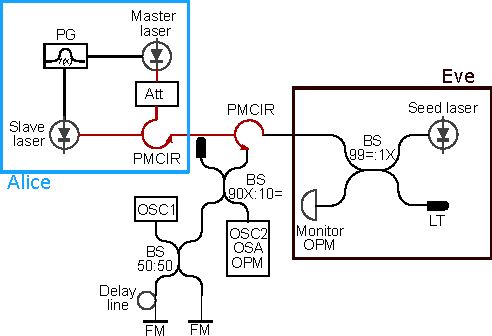
\includegraphics[width=0.9\textwidth]{images/setup_Faraday_Mirrors_final.pdf}
    \caption{Оптическая схема установки лазерного засеивания источника на основе оптической инжекции.}
    \label{fig:enter-label}
\end{figure}

В качестве источника были собраны два полупроводниковых лазера с распределенной обратной связью. Первый лазер - Agilecom WSLS-934010C4124-42 со встроенным изолятором, который использовался в качестве ведущего лазера для генерации опорного излучения. Второй же лазер представлял собой лазер Agilecom WSLS-934010C4124-82, аналогичный первому, но уже без встроенного изолятора. Это нужно для того, чтобы максимизировать количество изулчения, вводимого в резонатор ведомого лазера. Эти два лазера подключены друг к другу через оптический циркулятор. Первый порт его подключен в ведущему лазеру, излучение из которого попадает на второй порт циркулятора, куда подключен ведомый лазер. Таким образом изучение из лазера-мастера попадает в резонатор ведомого лазера. Излучение ведомого лазера попадает на второй вход циркулятора и проходит на третий порт циркулятора. В качестве источника мощного лазерного излучения использовался лазер Gooch \& Housego AA1406-193300 и волоконный эрбиевый усилитель. Для введения его излучения использовался дополнительный циркулятор, первый порт которого подключается к выходу усилителя, второй к третьему порту первого циркулятора. Для исследования интерференции полученных импульсов был собран волоконный интерферометр Майкельсона. 
\newline В ходе работы были исследованы характеристики выходных импульсов под действием внешнего излучения. Исследовались следующие параметры: амплитуда выходных импульсов и их стабильность, выраженная в измерении стандартного отклонения, длительность импульсов и их стандартное отклонение, а так же изучалась корреляция фазы  полученных импульсов с помощью волоконного интерферометра Майкельсона. В ходе воздействия изменялось стандартное отклонение энергии выходных импульсов в диапазоне от 2 до 3.5 процентов при мощности лазера атакующего в 900 мВт и при варьировании мощности лазера мастера.Результаты этих имзерений приведены на рисунке \ref{fig:area MDI ref}
\begin{figure}
    \centering
    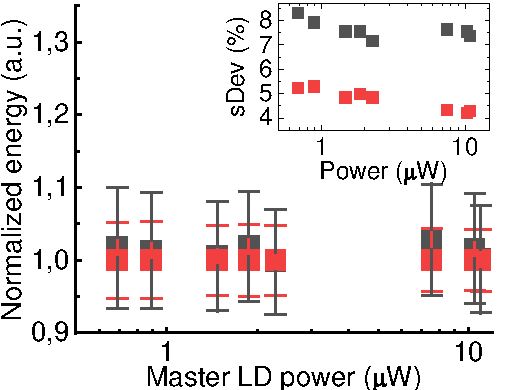
\includegraphics{images/area_under_attack.pdf}
    \caption{Изменение энергии импульса источника под действием внешнего излучения и без него в зависимости от мощности лазера-мастера.}
    \label{fig:area MDI ref}
\end{figure}
Данные результаты показывают, что Ева способна увеличивать нестабильность выходной мощности для увеличения среднего числа фотонах в импульсе. Длительность импульса так же изменяется под действием внешнего излучения, изображенном на рисунке \ref{fig:duration ref} Под внешним воздействием дрожание импульса возрастает на 2\%.  Существующие работы показывают, что даже незначительные отклонения в длительности импульса существенно снижают дальность распределения секретного ключа. 
\begin{figure}
    \centering
    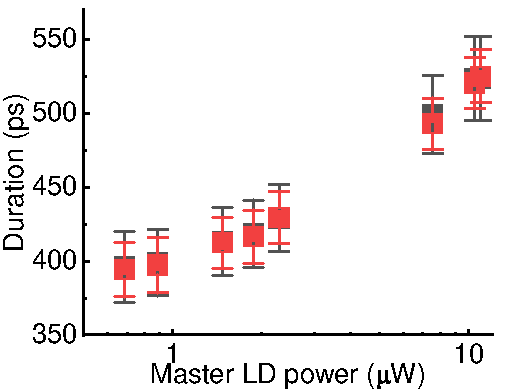
\includegraphics{images/duration_change.pdf}
    \caption{Измененение длительности импульса под действием внешнего излучения}
    \label{fig:duration ref}
\end{figure}
\newline Для разработки контрмеры необходимо рассчитать необходимый коэффициент изоляции для нааихудшего сценария, когда злоумышленник использует максимально доступную ему мощность. В непрерывном режиме эта величина составляет 2 Ватта. Эту величину необходимо ослабить до значения меньше -35 дБм. Благодаря использованию в составе схемы волоконно-оптического циркулятора, величина изоляции уже составляет 50 дБ.  Для рассчета необходимого значения аттенюации используется формула
\begin{equation}
\label{eq:isolation}
    \alpha = P_a - P_{req} - \beta
\end{equation}, где $\alpha$ - величина изоляции, которую необходимо внести, $P_a$ - величина зондирующей мощности в дБм, $P_{req}$ - мощность, до которой требуется ослабить входное излучение, $\beta$ - величина изоляции, которая уже реализована в схеме, в дБ. 
Подставим в \ref{eq:isolation} значения в 33 дБм мощности, что соответствует 2 Ваттам мощности и 50 дБ изоляции. В результате значение изоляции, необходимое для ослабления 2 Ватт до -35 дБм, равняется 18 дБ. Для обеспечения безопасности данного источника достаточно установить волоконный изолятор, типичная величина изоляции которого равна 30 дБ. Это перекроет весь допустимый диапазон зондирующих мощностей. 
\newline Полученные результаты демонстрируют стойкость предложенного источника когерентного излучения ко внешним воздействиям. Для изменения его характеристик злоумышленнику необходимо работать на мощностях, близких к мощностям, запускающих искру в волоконно-оптических линииях связи, что несет для него повышенные риски быть обнаруженным. А протоколы, основанные на протоколе с использованием недоверенного приемного узла обезопашены не только от атак злоумышленника на приемные узлы в виде детекторов одиночных фотонов, но так и от атак на источники одиночных фотонов.              % Реферат

\chapter*{Synopsis}
\addcontentsline{toc}{chapter}{Synopsis} 
\renewcommand{\figurename}{Figure}
\renewcommand{\thefigure}{\arabic{figure}} % Plain numbering
\setcounter{figure}{0}                     % Reset if needed

\begin{center}
    General thesis summary
\end{center}

\section*{Relevance}
Quantum key distribution (QKD) is a relevant technology emerging from quantum information science theory that allows a symmetric bit sequence to be distributed using quantum techniques to two or more users to use this sequence as a key for symmetric data encryption while simultaneously detecting unauthorized access by illegitimate users. The use of quantum states of light in the key distribution allows to achieve a level of secrecy unavailable to classical encryption protocols. Such quantum states can be represented as single photons. Their quantum properties do not allow an attacker to copy their states or read them without modification and without introducing errors. Such quantum states can be transmitted both through fiber-optic communication lines (FOCL), atmospheric channels and in outer space by means of satellites. The principle of operation of these systems is as follows. On the transmitter side (Alice) quantum states are formed. For this purpose coherent laser radiation is used, attenuated to single photons with the help of attenuator. A change in the polarization or phase shift of the photon is introduced into the prepared quants of light. The state thus prepared is transmitted through a communication channel to the receiver (Bob). At the receiver side, the photon state is re-measured independently of Alice. In the case of Bob's correlation, the received single photon is detected by a single photon detector. Due to the properties of the single photon in the form of impossibility of cloning, impossibility of measurement without destruction and its indivisibility it is possible to trace the impact of the intruder, as his actions will lead to the appearance of errors in the received bit sequence. This is how the control of unauthorized access is ensured. 

A separate class are systems of quantum key distribution on continuous variables (CV-QKD). In such systems quantum state, prepared and transmitted by Alice, on the receiving side interacts with strong laser radiation. And the result of this interaction is registered by a balance detector. The main differences of this detector from the detector of single photons is the use of two classical photodetectors, connected in such a way that their photocurrents are mutually subtracted, which reduces the noise of the system, and the lack of cooling to temperatures of about -40$^{\circ}$ degrees Celsius. All of this allows for simplification of the final system. To the advantages of the FACS can be attributed a greater speed of secret key generation compared to the FAC systems on discrete variables, which use single photon detectors. 

Among the complexities of the CV-QKD systems is the method of transmission of strong laser radiation or local oscillator (LO) to the receiving side and its separation from the quantum signal. In the first Gaussian modulated CV-QKD systems, the Local Oscillator and quantum states were generated at the transmitter, combined and transmitted together in a quantum channel. At the receiving end, the local oscillator and the quantum signal are separated, the LO is delayed by a special delay line and reconnected at the beam splitter for interaction. The result of this interaction is an interference pattern whose intensity distribution depends on the state encoded by Alice. The resulting field is registered by a balance detector, at the output of which a voltage level is formed, which is further subjected to post-processing.  Transmission of the local oscillator through the channel limits the range of operation of this type of system and limits the speed of key generation, because for the best operation of the system requires LO as much power as possible. The second problem is the ability of an attacker to manipulate the local oscillator to create information leakage channels. As an alternative, it is proposed to use a local oscillator generated at the receiving side. Such a solution will increase the range of key transmission, the speed of its generation and close the vulnerability to an attack on LO.
One of the promising approaches to the realization of quantum communication systems on continuous variables is the system of quantum communication on side frequencies of modulated radiation. The basis of this method is the transfer of the quantum channel to side frequencies, which appear as a result of modulation of optical radiation by an alternating electric field. This increases the stability of the transmitted signal to external influences and provides a high spectral efficiency, as well as provides indicators for the ratio of the rate of key generation to the distance between the receiver and transmitter units, comparable to other systems of quantum communication. This method is also suitable for realizing continuous variable protocols with coherent detection methods. In particular, this paper considers a heterodyne method in which the quantum states prepared by Alice are transmitted over a fiber link to the receiver, in it they fall on a 2$\times$2 beam splitter with a 50:50 splitting ratio and are mixed on it with a powerful local oscillator, which is detuned in frequency from the transmitting laser by an amount that exceeds the frequency of the state change. The result of the interference is detected by a balance detector. The output of the balance detector produces a signal at an intermediate frequency from the entire spectrum of the signal transmitted by Alice. Extraction of information requires filtering using low pass filter and demodulation of the received signal to generate a raw key. 

One of the challenges in implementing heterodyne detection method for key distribution is the need to compensate for phase noise. Various methods are used for this purpose. The first of these methods is the transmission of a 'pilot tone', during detection of which the phase noise contributed by the channel is measured. The measured value is then taken into account in the post-processing of the states. The second is the implementation of feedback in various forms. Within the scope of this paper, an optical feedback method is proposed for a quantum key distribution system at side frequencies on continuous variables. The essence of this method is the injection of laser radiation from the master laser, which is the transmitter laser, into the slave laser, which is used as a local oscillator in the receiver. This method allows stabilizing the LO wavelength and reducing phase noise due to the fact that both sources are coherent radiation generators with random phase.
The optical injection method requires an additional channel to transmit the feedback generation. Such a channel increases system complexity and fiber optic link (FOCL) requirements, which is particularly critical in urban links where the allocation of an additional fiber or channel in multiplexed networks is difficult. The solution to this problem may be a system of quantum key distribution on continuous variables using heterodyne detection with independent LO. The essence of this system is that the receiver and transmitter are equipped with wavelength stabilized lasers with a spectral line width of less than 10 kHz. This approach allows to avoid constant adjustment of the laser wavelengths and to reduce the phase noise associated with the independence of the radiation sources.
However, the phase noise does not disappear, so it still needs to be compensated. In the case of implementing such a signal detection method for a quantum key distribution protocol at side frequencies, the carrier frequency can be used for this purpose by measuring its phase and making adjustments in post-processing. 

The differences between real QKD systems and the models used for theoretical proofs can be exploited by an attacker to carry out different types of attacks on the equipment comprising the system. It has been shown in earlier works that laser radiation sources based on semiconductor crystals can be vulnerable to 'seeding' by an attacker's external radiation at a wavelength close to that used by the transmitter. This attack results in a change in the shape of the emitted pulse and an increase in output power, and in some cases a change in wavelength can also be observed. These effects result in an increase in the average number of photons emitted by the transmitter, which opens up the possibility of a photon number splitting attack for the attacker. 
However, 'seeding' attacks by laser radiation at other wavelengths have not been considered in the literature. This type of attack is more dangerous because passive fiber optic elements that introduce additional attenuation, such as isolators or DWDM filters, are used to protect against it. However, there are works that demonstrate that the amount of attenuation in such elements can be reduced when the incident wavelength of the radiation is significantly changed. For example, an insulator with an operating wavelength of 1550 nm introduces 50 dB of back-pass loss, when this value is 20 dB when exposed to radiation at a wavelength of 1310 nm. And in the case of the DWDM filter, it contributes virtually no attenuation at 1310 nm. Thus, it is much easier for an attacker to perform a 'seeding' attack with laser radiation, since the attenuation introduced at this wavelength is less. 

This type of attack is called an 'optical pumping attack'. Its essence is that the attacker probes the laser with a wavelength different from the operating wavelength. This radiation is absorbed by the active medium of the transmitter laser so that the absorbed radiation acts as an optical pump, which works as a complement to the electrical pump of the semiconductor laser. In this case, the Watt-Ampere characteristic of the laser and its quantum efficiency changes. This leads to the fact that the energy of the emitted pulses increases while the pump current remains unchanged. In the framework of this work, this type of attack is first labelled, the lower limit of the necessary radiation power at the wavelength of 1310 nm to change the characteristics of the laser under study is determined, and the effect of optical pumping on the laser characteristics is measured. 

In quantum distribution systems, laser radiation sources based on optical injection are used. Such sources are constructed in the following way: two lasers are used -- a master and a slave laser connected by a circulator. Radiation of the slave laser allows reducing the jitter of emitted pulses, stabilizing the output power and narrowing the spectral line. However, such sources have not been investigated for robustness to external radiation. Previously shown work on laser 'seeding' has been carried out only for single radiation sources. A source based on optical injection has several advantages relative to a single source: the presence of isolation from the quantum channel due to the optical circulator and the presence of external radiation from the leading laser. This work studies the effect of high-power laser radiation on the duration, jitter, and amplitude of the emitted pulses, and demonstrates a lower bound on the radiation power required to modify the operation of this system.

\section*{The goal of the research}

To develop a system of heterodyne detection of signals in a quantum communication system at side frequencies with a local oscillator on the receiver side using optical injection and to investigate the resistance to attacks on the technical implementation of laser radiation sources in this system.
In order to achieve the goal in the framework of the thesis, the following objectives have been established:
\section*{Objectives of the research}
\textbf{Objective 1: development of QKD system with feedback}\\
Implementation of optical injection feedback for sideband QKD system with heterodyne detection method and continuous variables\\

\textbf{Objective 2: research of heterodyne detectinon for SCW-QKD with two independent sources} \\
Application of heterodyne signal detection in QKD systems with two independent sources of laser radiaton and development of polartzation maitaining algorithm.\\

\textbf{Objective 3: experimental design}\\
Study the optical pumping attack on radiation sources that can be local oscillators for continuous variable quantum key distribution systems.\\

\textbf{Objective 4: research of influence of high power radiation to optical injection locked source.}\\
To investigate the effect of high-power optical radiation on a radiation source based on optical injection.
\section*{The novelty of research}
An optical injection feedback system for a quantum key distribution system at side frequencies is implemented for the first time and the sifted key is transmitted. A heterodyne signal detection method with two independent radiation sources is implemented for a quantum key distribution system at side frequencies and a polarization control algorithm is developed for this system. For the first time a new type of attack on the technical implementation - optical pumping attack on the radiation source in quantum key distribution systems, which allows to increase the emitted average number of photons bypassing the existing protection methods, is demonstrated. The influence of high-power laser radiation on the source of coherent radiation based on optical injection has been determined experimentally, which increases the energy of emitted pulses and its spread, increases the output power of the attacked source, which together leads to a decrease in the rate of secret key generation.

\section*{Theoretical and pratcical significance}

The theoretical significance of the work is determined by the fact that within the framework of it phase-encoded states in the system of quantum key distribution at side frequencies on continuous variables with heterodyne method of signal detection were transferred and the wavelengths of information laser and local oscillator laser were stabilized. Also within the framework of the work the exchange of phase-encoded states in the system of quantum distribution of keys at side frequencies on continuous variables with heterodyne method of signal detection and two independent sources of radiation of information signal and local oscillator was made, within the framework of transfer of such states the algorithm of adjustment of polarization of information radiation was worked out. The average output power and pulse energy of a distributed feedback laser used in quantum key distribution systems are increased by optical pumping at a wavelength of 1310 nm. The average output power and standard deviation of the amplitude of the output pulses emitted by a coherent radiation source based on optical injection with the help of high-power laser radiation of an intruder, leading to the creation of additional vulnerability on access to the secret key, is increased. 
Practical significance of the work lies in the fact that the conducted experimental studies on the implementation of heterodyne method of signal detection show the operability of this approach to create systems of quantum key distribution using this method of signal registration. Researched methods of the attacker's influence on the sources of radiation in the systems of quantum key distribution allows to improve the model of the intruder, increasing the resistance of the final systems of quantum key distribution to attacks on the technical implementation


\section*{Assertions that are presented for defense}
\begin{enumerate}
    \item Transmission of phase-coded signals in a continuous-variable quantum key distribution system with a heterodyne signal detection method and a local oscillator implemented at the receiver end becomes possible by stabilizing the wavelengths of the radiation sources used through the use of optical injection to implement feedback.
    \item An algorithm that involves monitoring the polarization of the incoming signal, based on an analysis of the spectral composition of the electrical signal obtained after a Fast Fourier Transform, and with polarization rotation based on this analysis, enables the exchange of phase-coded states in a quantum communication system at sidebands using continuous variables and a heterodyne signal detection method based on two independent laser radiation sources in the telecommunications wavelength range and using frequency multiplexing on a single carrier frequency.
    \item Absorption of an intruder's laser radiation by the active medium of a distributed-feedback semiconductor laser used in a quantum key distribution system transmitter increases the average number of photons emitted by it.
    \item Seeding a slave laser in a light source based on the optical injection method with an intruder's laser operating in continuous mode, with a power of at least 800 mW and a wavelength matched to the wavelength of the slave laser, increases the standard deviation of the slave laser's output pulse amplitude by $3\%$, increases the standard deviation of their energy by $3\%$, increases the standard deviation of pulse duration by $2.5\%$, and increases the average emitted power by $8\%$, resulting in a reduction in the secret key transmission range by $10\%$.
\end{enumerate}

\section*{Approbation of research results}
Key research results were presented and discussed at the following conferences:
\begin{enumerate}
    \item CYS X 'Application of the heterodyne signal analysis method for implementing a quantum communication protocol with a star topology'
    \item IWQO-2021 'Application of the heterodyne signal analysis method for implementing a quantum communication protocol with a star topology'
    \item PPS LI 'Coherent reception in quantum communication systems at side frequencies with an untrusted receiving node'
    \item XI CYS 'Multi-user city-scale quantum networks based on passive optical networks'
    \item 20th International Conference Laser Optics ICLO 2022 'Continuous variable measurement-device-independent quantum communication scheme based on subcarrier waves'
    \item XII CYS 'Quantum communication system on continuous variables with an untrusted receiving node'
    \item LII scientific and educational-methodological conference of the teaching staff 'Frequency multiplexing for a quantum key distribution system on side frequencies'
    \item All-Russian scientific conference with international participation 'Nevskaya Photonics-2023' (09.10.2023 - 13.10.2023), 'Heterodyne detection for a quantum key distribution system at side frequencies with two independent radiation sources'
    \item 22nd International Conference Laser Optics ICLO 2024 'Laser-pumping attack on QKD sources', 1-5 July 2024
    \item 22nd International Conference Laser Optics ICLO 2024, 'Secure laser source for QKD systems', 1-5 July 2024
    \item QCrypt 2024, 2-6 September 2024, 'Optical pumping attack to laser source in Quantum key distribution system'
\end{enumerate}

\section*{Validity of scientific results}
The reliability of the obtained results is based on the use of modern methods of scientific research and comparison of the obtained results with the data of scientific and technical literature. The approved methods and certified equipment were used in the research. Experimental data processing was carried out with the help of Origin and Python application software package. The materials were published in 9 printed papers and presented at 10 international and Russian conferences.

\section*{Implementation of research results}
The results of the dissertation work have been implemented in projects carried out within the framework of the Roadmap in the direction of "Quantum Communications", such as "Development and creation of a quantum communication system on continuous variables", which implemented the results obtained in the implementation of a heterodyne detection method for a quantum key distribution system on side frequencies and "Creation of a Pilot Section of the Backbone Quantum Network", which implemented research into the resistance of a laser radiation source to an attack by optical pumping.

\section*{Personal contribution of the author}
The graduate student personally developed optical circuits for quantum key distribution systems at sidebands using a heterodyne signal detection method and optical injection. He also investigated the effect of optical pumping on a laser with distributed feedback and the effect of high-power optical radiation on optical injection-based radiation sources. The graduate student conducted experimental work to study the operation of the developed systems and independently processed the experimental results.
\section*{Publications}
Key results of research are described in nine publications. Nine of them are  published in a journal indexed by Scopus. Four patents for inventions has also been obtained.\\

\section*{Thesis structure and number of pages} The dissertation consists of an introduction, four chapters, conclusion and two appendices. The full dissertation 309 pages long, including \totalfigures\ figures and \totaltables\ tables. The bibliography contains 120 titles.

\section*{The main content of the work}
In the \underline{introduction} the relevance of the research conducted within the framework of the thesis work is justified, the purpose of the research is defined, the tasks of the work are set, the scientific novelty of the work, its theoretical and practical significance, as well as the possibility of implementation of its results are indicated. 
In the \newline In the \underline{first chapter} is given a review of the state of science and technology on the subject of quantum key distribution. Quantum communication protocols using both discrete and continuous variable are considered. The features of coherent detection methods used in quantum key distribution systems are described and analyzed. The issue of phase noise in quantum key distribution systems is highlighted. Examples of methods to compensate for phase noise are demonstrated, such as applying pilot pulses and creating feedback.  Known attacker's attacks on equipment within QKD systems are demonstrated. The laser seeding attack on the transmitter laser, its impact and possible defense methods are described. Another aspect under consideration is an attack on the power of the local oscillator transmitted in the channel for quantum key distribution systems on continuous variables, the principle of its implementation, the result of the attack and methods to counteract it.
\newline In the \underline{second chapter}, we investigate the optical injection method. The optical injection method is that there is a pair of lasers: a master laser and a slave laser. The radiation from the master laser is injected into the resonator of the slave laser. Injection of additional photons into the resonator of the slave laser reduces the relaxation oscillation time of the radiation, which accelerates the radiation generation process and reduces negative effects. This approach improves the emission characteristics of the slave laser in particular:
\begin{itemize}
    \item narrowing of the spectral line of the output radiation
    \item Reduction of nonlinearities and suppression of relaxation oscillations
    \item Reducing the output pulse chirp and increasing amplitude stability
\end{itemize}
This approach allows synchronizing the frequencies of the master and slave lasers, and as a consequence, reducing their relative phase noise, achieving phase synchronism. This effect allows optical injection to be used as a feedback implementation for the local oscillator in a QRC system at side frequencies using continuous variables. The result of the feedback application will be stabilization of the intermediate frequency and reduction of phase noise. To implement this method, a separate channel and circulator is used to separate the radiation of the master and slave laser. 
This method can be applied to a quantum key distribution system at side frequencies.
\begin{figure}
    \centering
    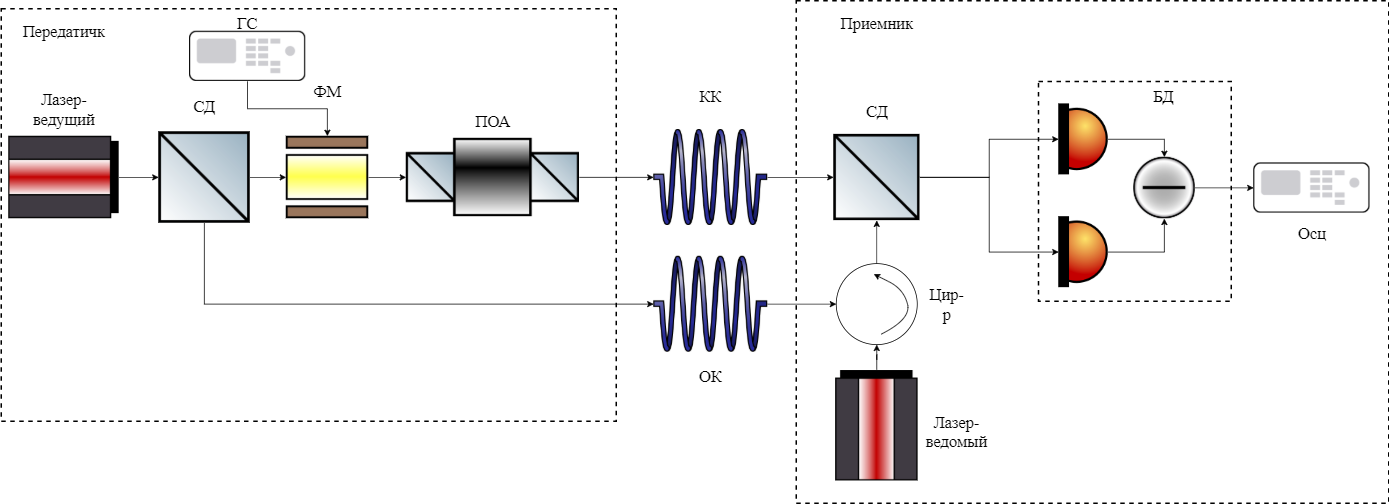
\includegraphics[width=\textwidth]{images/Схема с обратной связью.png}
    \caption{Schematic diagram of the QKD system experiment using optical injection. SD - beam splitter, FM - phase modulator, GS - signal generator, POA - tunable optical attenuator, QC - quantum channel, OC - open channel, Qir-r - circulator, BD - balance detector, Osz - oscilloscope}.
    \label{fig:opt inj scheme syn}
\end{figure}
This system, the optical scheme of which is shown in Figure~\ref{fig:opt inj scheme syn}, works as follows. At the transmitter side, the radiation generated by the laser is split into two parts. The first part of the radiation goes to an Alice phase modulator, where phase modulation by an alternating electrical signal takes place, in which phase shifts are introduced to encode the information. Quadrature Phase Shift Keying or Quadrature Phase Shift Keying (QPSK) modulation can be used as encoding. This digital modulation method introduces phase shifts corresponding to values of 45\textdegree, 135\textdegree, 225\textdegree and 315\textdegree. These phase shift values are assigned bit values {00, 01, 10, 11}. As a result, three harmonics of the signal appear in the spectrum: $\omega$ - the centre frequency of the laser, $\omega$ - $\Omega$ - the lower side frequency and $\omega$ + $\Omega$ - the upper side frequency, where $\Omega$ is the modulation frequency. The radiation after modulation is described by Eq:
\begin{align}
\label{eq:spectrum seed syn}
F_s(t) & = A_0 * \sin(\omega_0 t + \phi_0) + \frac{A_0 * m}{2} * (\sin((\omega_0 + \Omega)t + (\phi_0 + \phi (t))) - \notag \\\
&- \frac{A_0 * m}{2} * (\sin((\omega_0 - \Omega)t + (\phi_0 - \phi (t)))),
\end{align} where $A_0$ is the amplitude of the original radiation, $\omega$ is the centre frequency of the laser, $\omega$ - $\Omega$ is the lower side frequency and $\omega$ + $\Omega$ is the upper side frequency, $\Omega$ is the modulation frequency, $\phi_0$ is the phase of the original radiation, $\phi(t)$ is the phase of the modulating radiation, $t$ is the time, $m$ is the modulation index. Modulation index is the value of the ratio of power at side frequencies to the power in the whole spectrum. The modulation index is proportional to the amplitude of the modulating electrical signal.  The obtained spectrum falls on a variable optical attenuator, the attenuation of which is adjusted in such a way that at the side frequencies there is a power corresponding to a given average number of photons, when the carrier can remain classical. The prepared quantum states are transmitted into the quantum channel. 
The second part of the radiation passes through a separate fiber channel to the receiver side, where it enters the fiber circulator so that the radiation enters the slave laser resonator. 
The incoming radiation from the quantum channel enters the first input of a fiber beam splitter with two inputs and two outputs and a 50:50 splitting ratio. The second input of the beam splitter is a local oscillator, which is the radiation generated by a separate laser on the receiving side. Due to the presence of feedback in the form of optical injection, the wavelength of the laser on the receiving side is synchronized with the wavelength of the Alice laser. As a result, the LO and quantum states interfere at the beam splitter. As a result of this interference, additional harmonics at an intermediate frequency appear at the output of the beam splitter. These harmonics are $\omega$ - $f$ - the central frequency of the Alice laser minus the LO frequency, ($\omega$ - $\Omega$) - $f$ - the lower side frequency minus the LO frequency and ($\omega$ + $\Omega$) - $f$ - the upper side frequency minus the LO frequency, where $\Omega$ - the modulation frequency, $\omega$ - the Alice laser frequency, $f$ - the LO frequency. 
\newline The result of this interference is detected by a balance detector. This device is two classical photodiodes connected so that their currents are subtracted. This connection reduces the intrinsic noise of the detector. After that, the received current is passed to a low-pass filter to filter out the constant component. The resulting signal is amplified by an amplifier stage and sent to the ADC.  As a result, only one signal is formed at the output of the balance detector at the frequency coinciding with the modulation frequency on the transmitter side. The reason for this is that the wavelengths of the LO and the transmitter laser coincide due to feedback in the form of optical injection. Thus, only the ($\omega$ + $\Omega$) component $f$ remains at the detector output, and the rest is converted to a constant component, which is filtered out. 
\begin{figure}
    \centering
    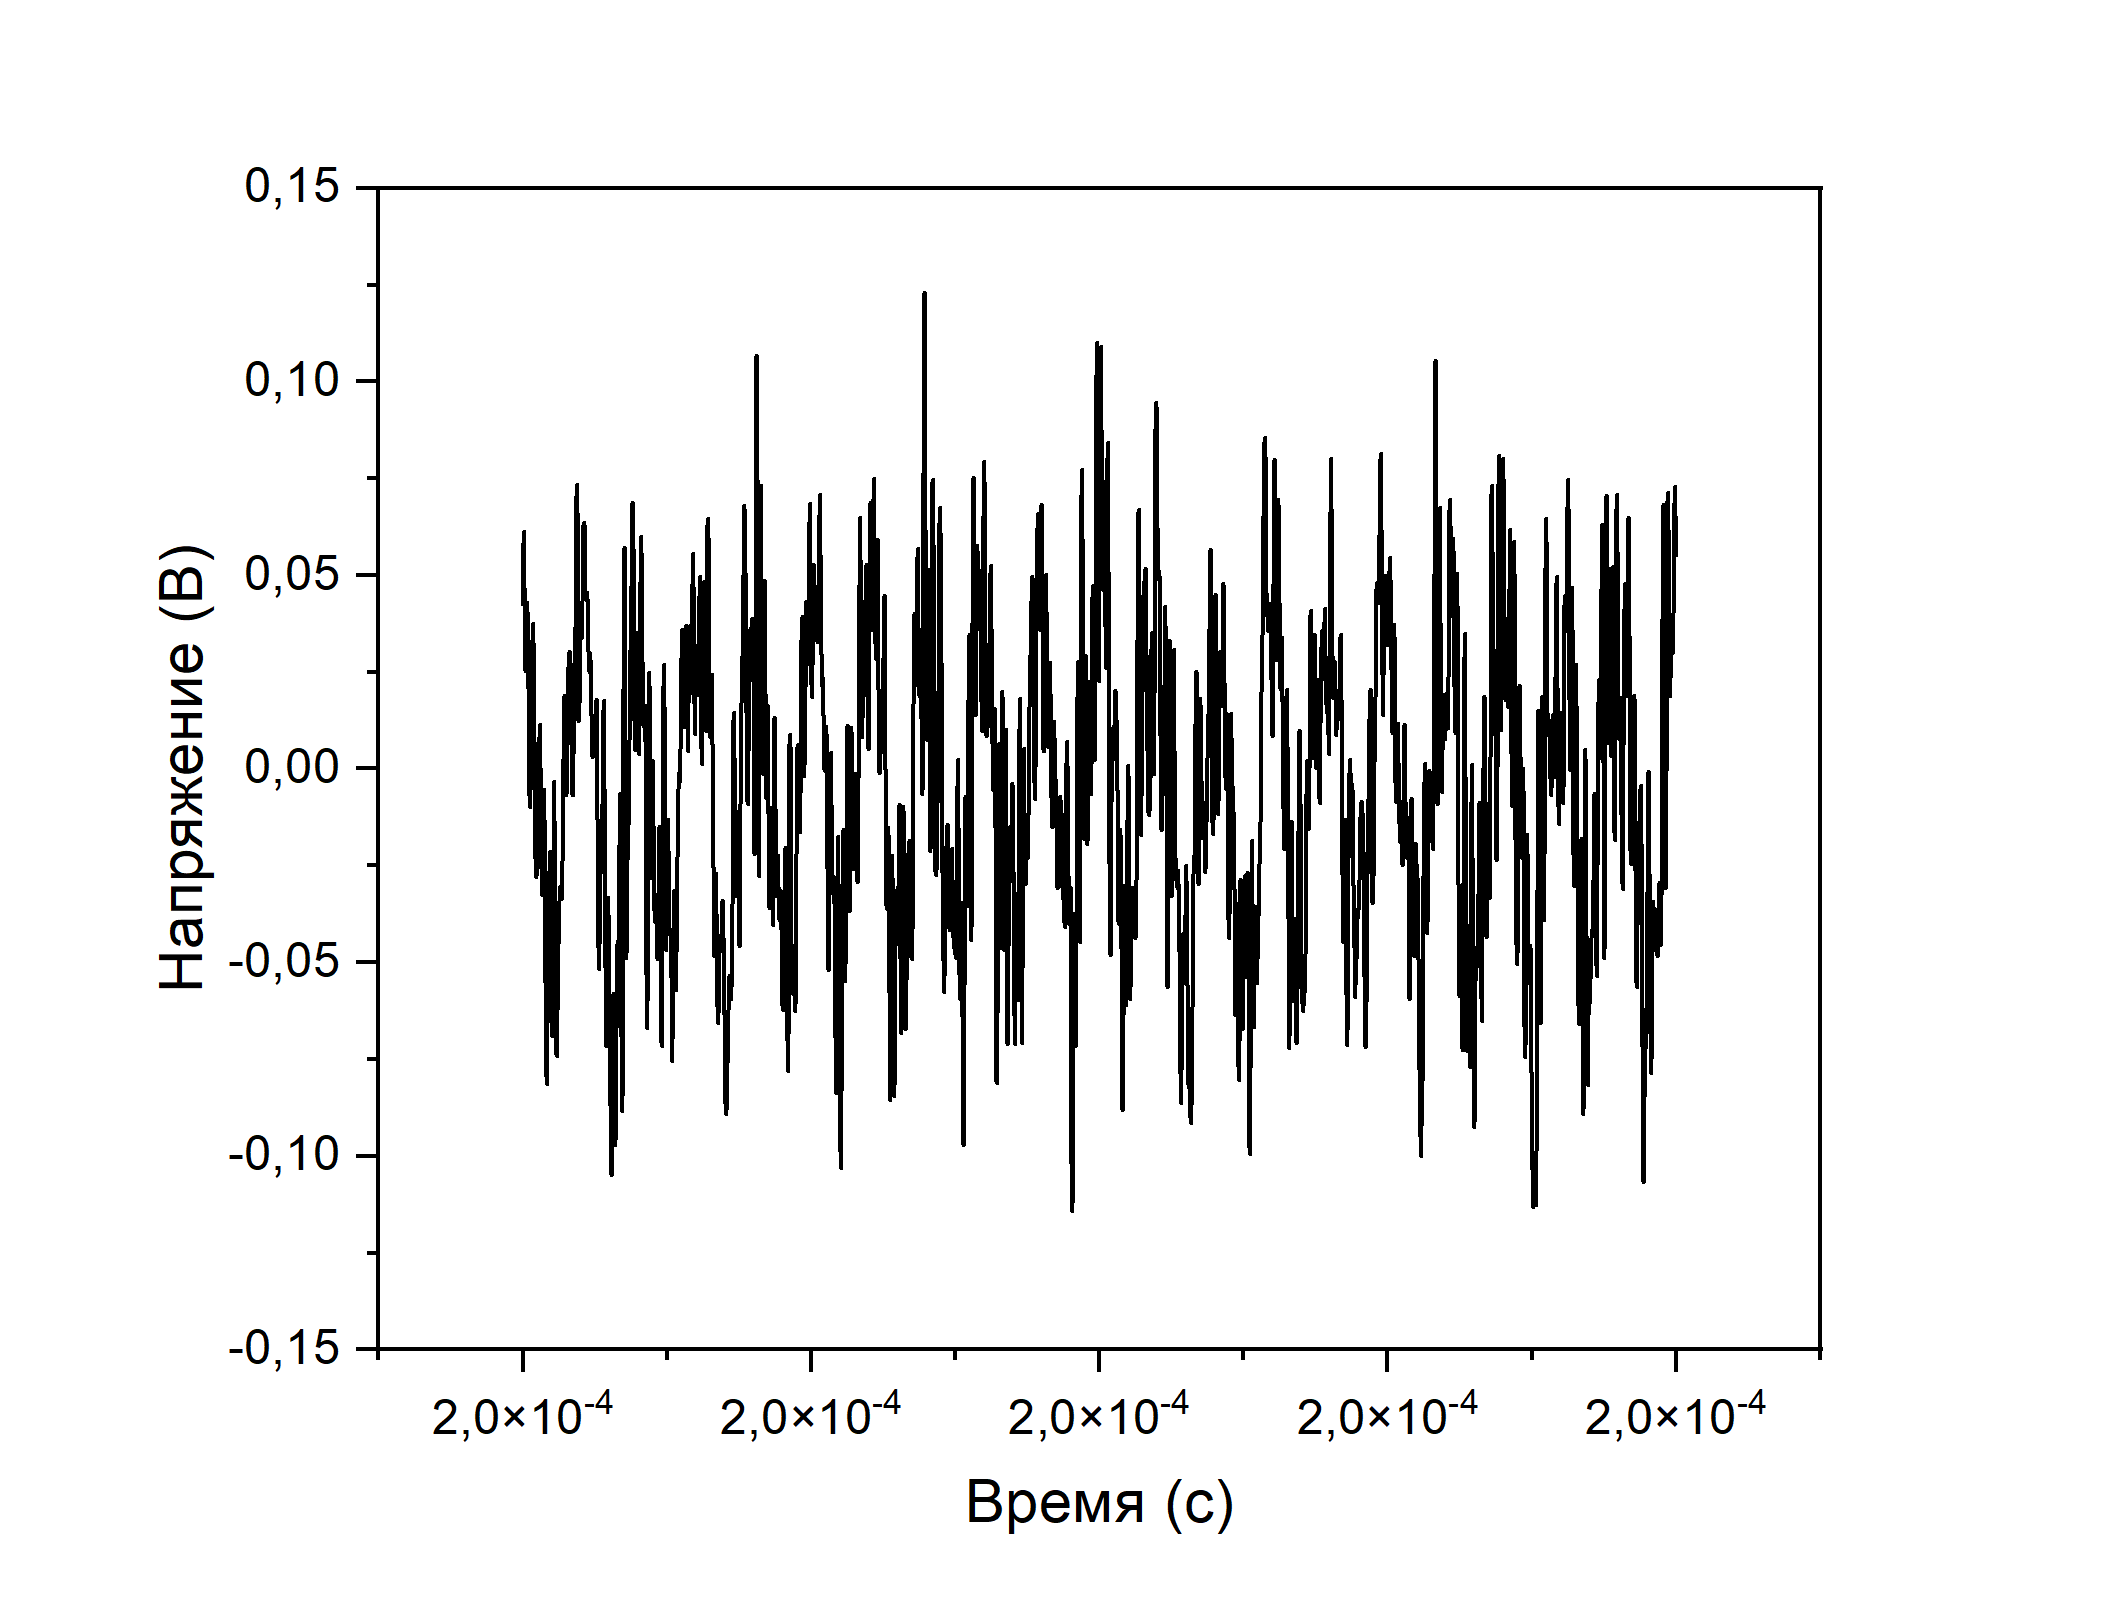
\includegraphics[width=\textwidth]{images/03.png}
    \caption{Noisy signal at the output of a balanced detector}
    \label{fig:noisy output inject syn}
\end{figure}
The received oscillation at the output of the balance detector carries phase information encoded by Alice. This signal is processed by digital signal processing techniques to extract the phase value of the signal. 
\begin{figure}
    \centering
    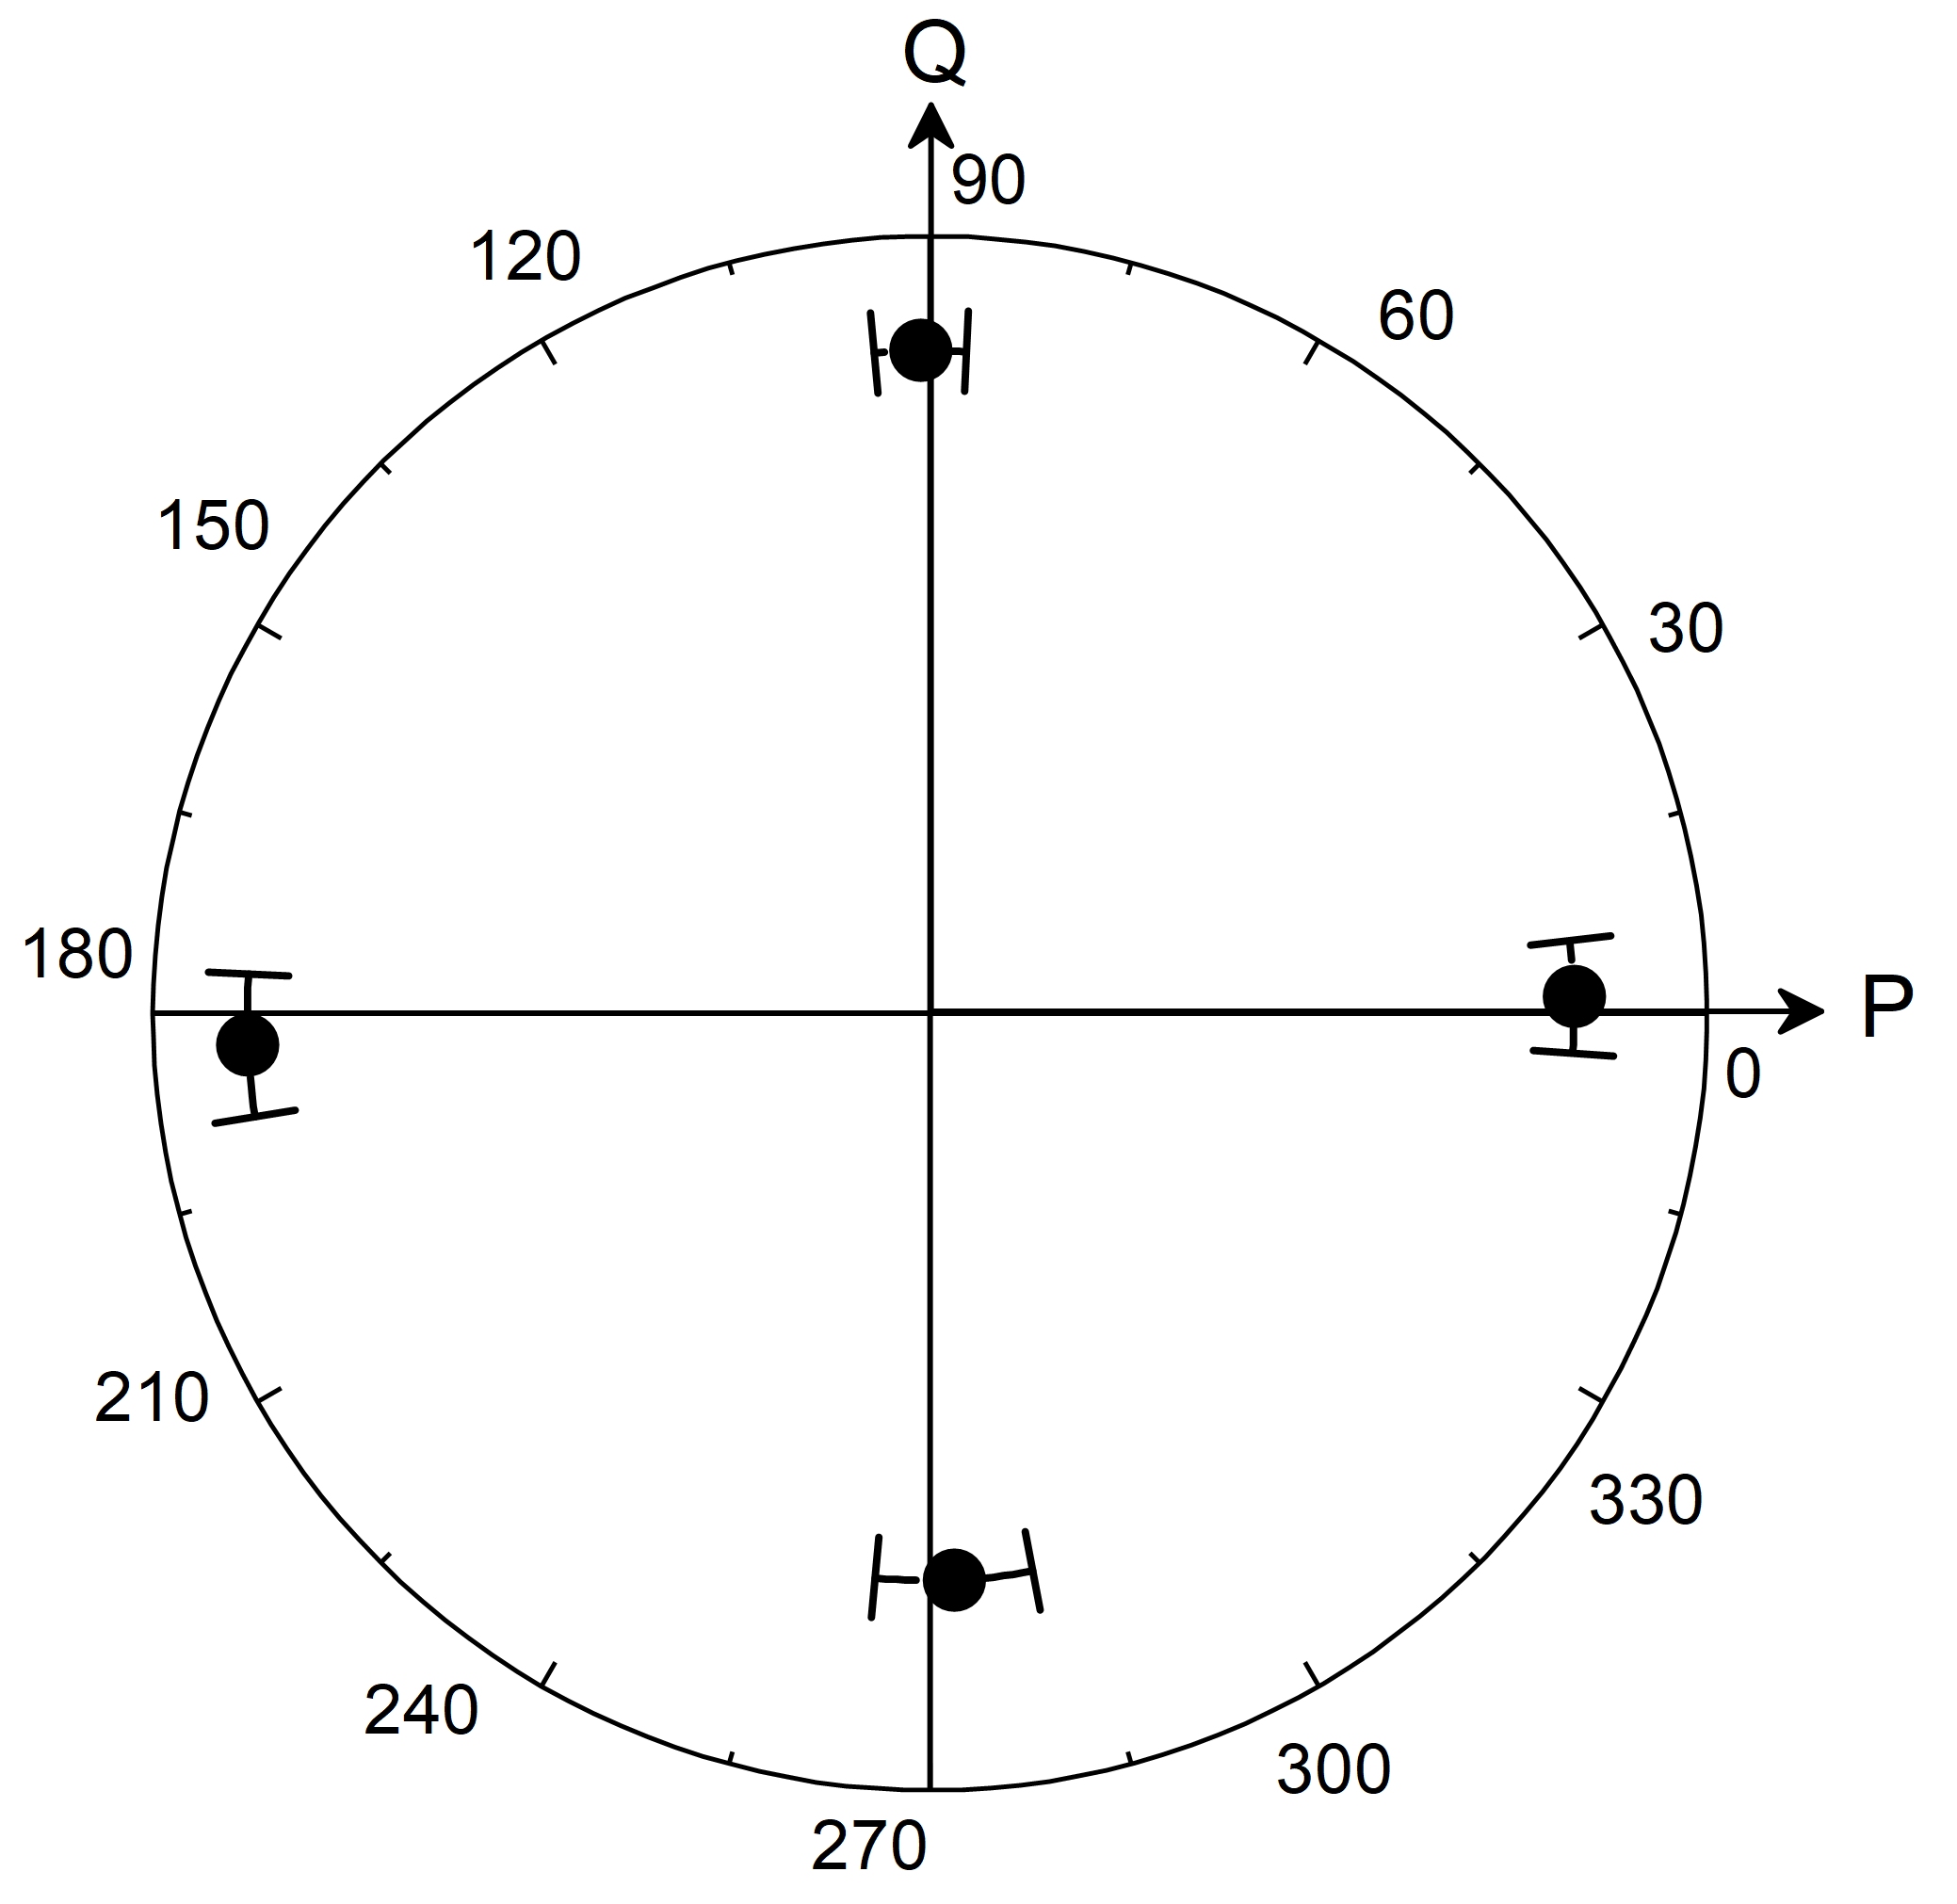
\includegraphics[width=0.8\textwidth]{new_iq_graph_het_true.png}
    \caption{Phase values obtained after digitalisation}
    \label{fig:phase meas ijnect syn}
\end{figure}

The resulting bit sequence is the raw key. The received key is sifted. In the obtained sifted key, the quantum bit error rate (QBER) is estimated by first opening a part of the key. And the last step is secrecy amplification using HASH functions.
To the pluses of this method of realisation of the QKD can be attributed the simplicity of the system, due to the fact that there is no active selection of the basis in the form of a modulator of any type. The presence of feedback in the form of optical injection allows to solve several problems: stabilisation of the LO wavelength, which also simplifies the final system, and reduces phase noise associated with the randomness of the phase of laser radiation generated by different sources. The use of heterodyne method of reception allows to use any type of modulation, which allows to flexibly adjust the protocol for different tasks and leaves the future for increasing the speed of key generation.
\newline The disadvantages of this system include the need for an additional fibre-optic communication channel for feedback, which is partially offset by the fact that real QKD systems are embedded into existing data transmission systems that work with multiplexing technology and the optical injection signal can be embedded into already used channels, as it has no requirements to the level of third-party noise. The second drawback, however, is the vulnerability to laser seeding attack, which requires further study and countermeasures. 
\newpage In the \underline{third chapter}, a scheme for applying the heterodyne detection method to detect signals with two independent signal sources for a quantum communication protocol at side frequencies is discussed. A feature of this system is the transfer of quantum states of light to side frequencies that appear in the emission spectrum. The basic implementation of this protocol involves the use of discrete variables and single photon detectors based on avalanche photodiodes for signal registration. However, it is possible to adapt this protocol to use coherent detection methods. 
\newline In this paper we propose the use of heterodyne signal detection method for a quantum communication system at side frequencies.
\begin{figure}
    \centering
    \includegraphics[width=\textwidth]{Гетеродин схема новая2 .png}
    \caption{Scheme of a quantum key distribution system at side frequencies with an independent local oscillator. SD - beam splitter, FM - phase modulator, GS - signal generator, POA - tunable optical attenuator, QC - quantum channel, BD - balance detector, Osz - oscilloscope}.
    \label{fig:het true scheme syn}
\end{figure}
This system works as follows. A laser on the transmitting side generates coherent radiation. This radiation, having passed through the necessary passive elements in the form of optical isolators, reaches the crystal of the phase modulator. An alternating voltage at the modulation frequency is transmitted to the electrical input of the phase modulator. A phase shift is introduced into this voltage, which corresponds to bits of information. Quadrature phase-shift keying or quadrature phase-shift keying (QPSK) is used as an example in this paper. The phase shift values in this case are {45\textdegree, 135\textdegree, 225\textdegree and 315\textdegree} and the following information bits {00, 01, 10, 11} correspond to these phase shifts. As a result of this modulation, three harmonics appear in the spectrum of radiation after the phase modulator, two of which encode information from the transmitter. The prepared radiation is attenuated by a variable attenuator to achieve a power level at side frequencies less than 1 photon on average. The quantum states thus obtained are transmitted via a fiber optic communication line to the receiving side.  
\newline The transmitted signal from Alice, after passing through the fiber optic link, reaches the polarization controller to compensate for the distortions introduced by the passage through the fiber. After that, the polarization beam splitter is installed and only the desired polarization is selected and the radiation with the desired polarization is allowed to pass through. The quantum states are then mixed with the LO generated by a separate laser on a beam splitter with two inputs and two outputs and a 50:50 splitting ratio. These signals interfere and as a result of this interference, the emission spectrum is enriched with additional harmonics. These harmonics appear because the frequencies of the LO and the Alice laser do not match. These spectral components are at different frequencies - total, difference and Raman. But given the limited bandwidth of the balance detector, we can observe at its output only harmonics at difference frequencies that fall into it. Total and other combinational frequencies do not fall into the bandwidth of the DB and are registered as a constant component, which loses all the information encoded in their phases. Where as the harmonic oscillations at the difference intermediate frequency pass the amplifying stage unchanged and retain the information encoded in the phase of Alice's emission. In this way, the spectrum is transferred from the optical domain to the radio frequency domain, where amplification and signal processing are simplified.
\begin{figure}
    \centering
    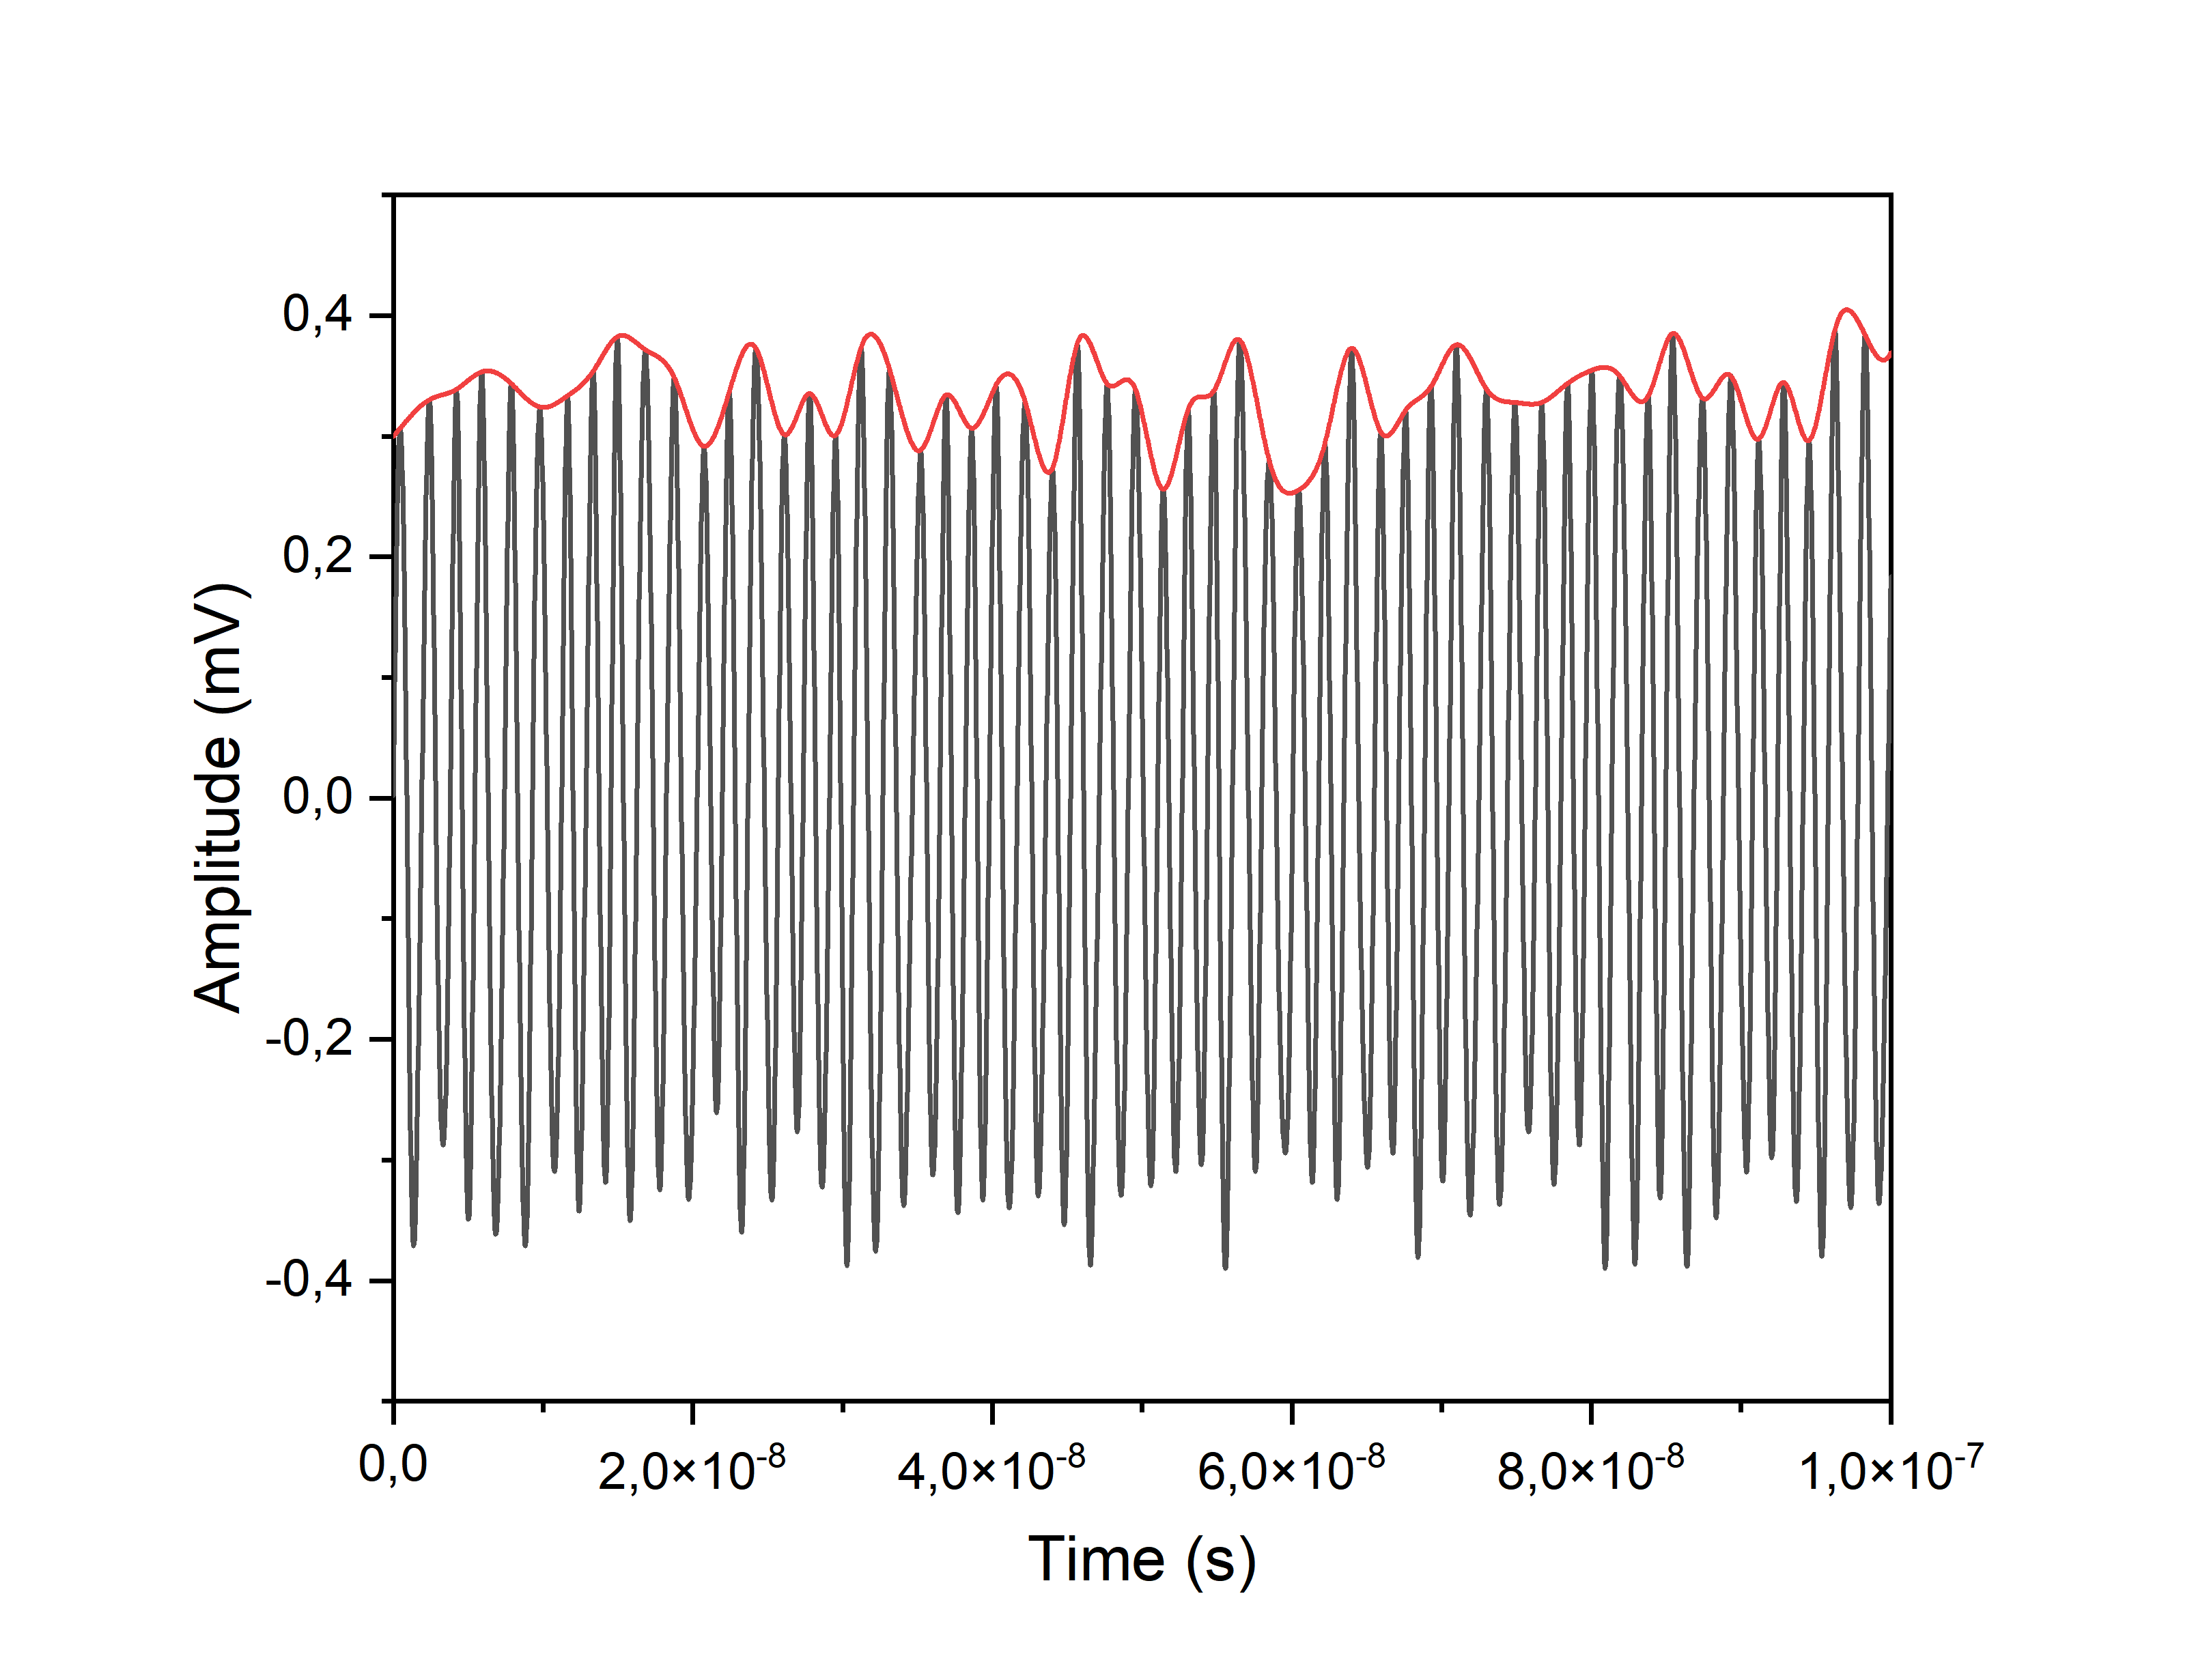
\includegraphics[width=\textwidth]{images/balanced output heterodyne.png}
    \caption{The signal at the output of the balanced detector after heterodyne reception}.
    \label{fig:het time output syn}
\end{figure}
\newline A balance detector is a device that consists of two photodetectors connected so that their photocurrents are mutually subtracted. The received signal is then filtered to eliminate the influence of the constant component of the photocurrent. After that the received signal goes to the amplifier stage to increase its amplitude. The presence of the amplifier stage limits the bandwidth of the entire device. Typical bandwidths can vary from 100 MHz to 1.2 GHz. This limits the range of received frequencies and the raw key generation rate. 
\newline The received signal after amplification must be digitised by an ADC for further processing. As processing can be applied various methods of digital signal processing, such as Fast Fourier Transform or Hilbert Transform. As a result of this processing, phase values are generated from the harmonic signal received after the ADC, which correspond to given bit values from which a bit sequence called raw key is formed. 
However, using LO at the receiver side requires tweaking its polarisation and the polarisation of the quantum states for effective interference at the receiver. In this work, a polarisation control algorithm based on Fast Fourier Transform is proposed. The essence of this algorithm is that when a polarisation beam splitter is used, the modulation frequency that carries the information from the transmitter is doubled.
This appearance of the doubled frequency can be tracked in the frequency domain. The following algorithm is used for this purpose 
\begin{enumerate}
    \item Apply FFT to the received signal
    \item Analyse the spectral composition of the signal
    \item Rotating the polarisation of the signal until the harmonic is eliminated at twice the modulation frequency.
    \item Further rotation of the signal polarisation to the harmonic maximum at the modulation frequency
\end{enumerate}
As a result of its operation, it is possible to adjust the polarisation by using active polarisation control, which will use the FFT result as feedback to adjust the polarisation. 
\begin{figure}
    \centering
    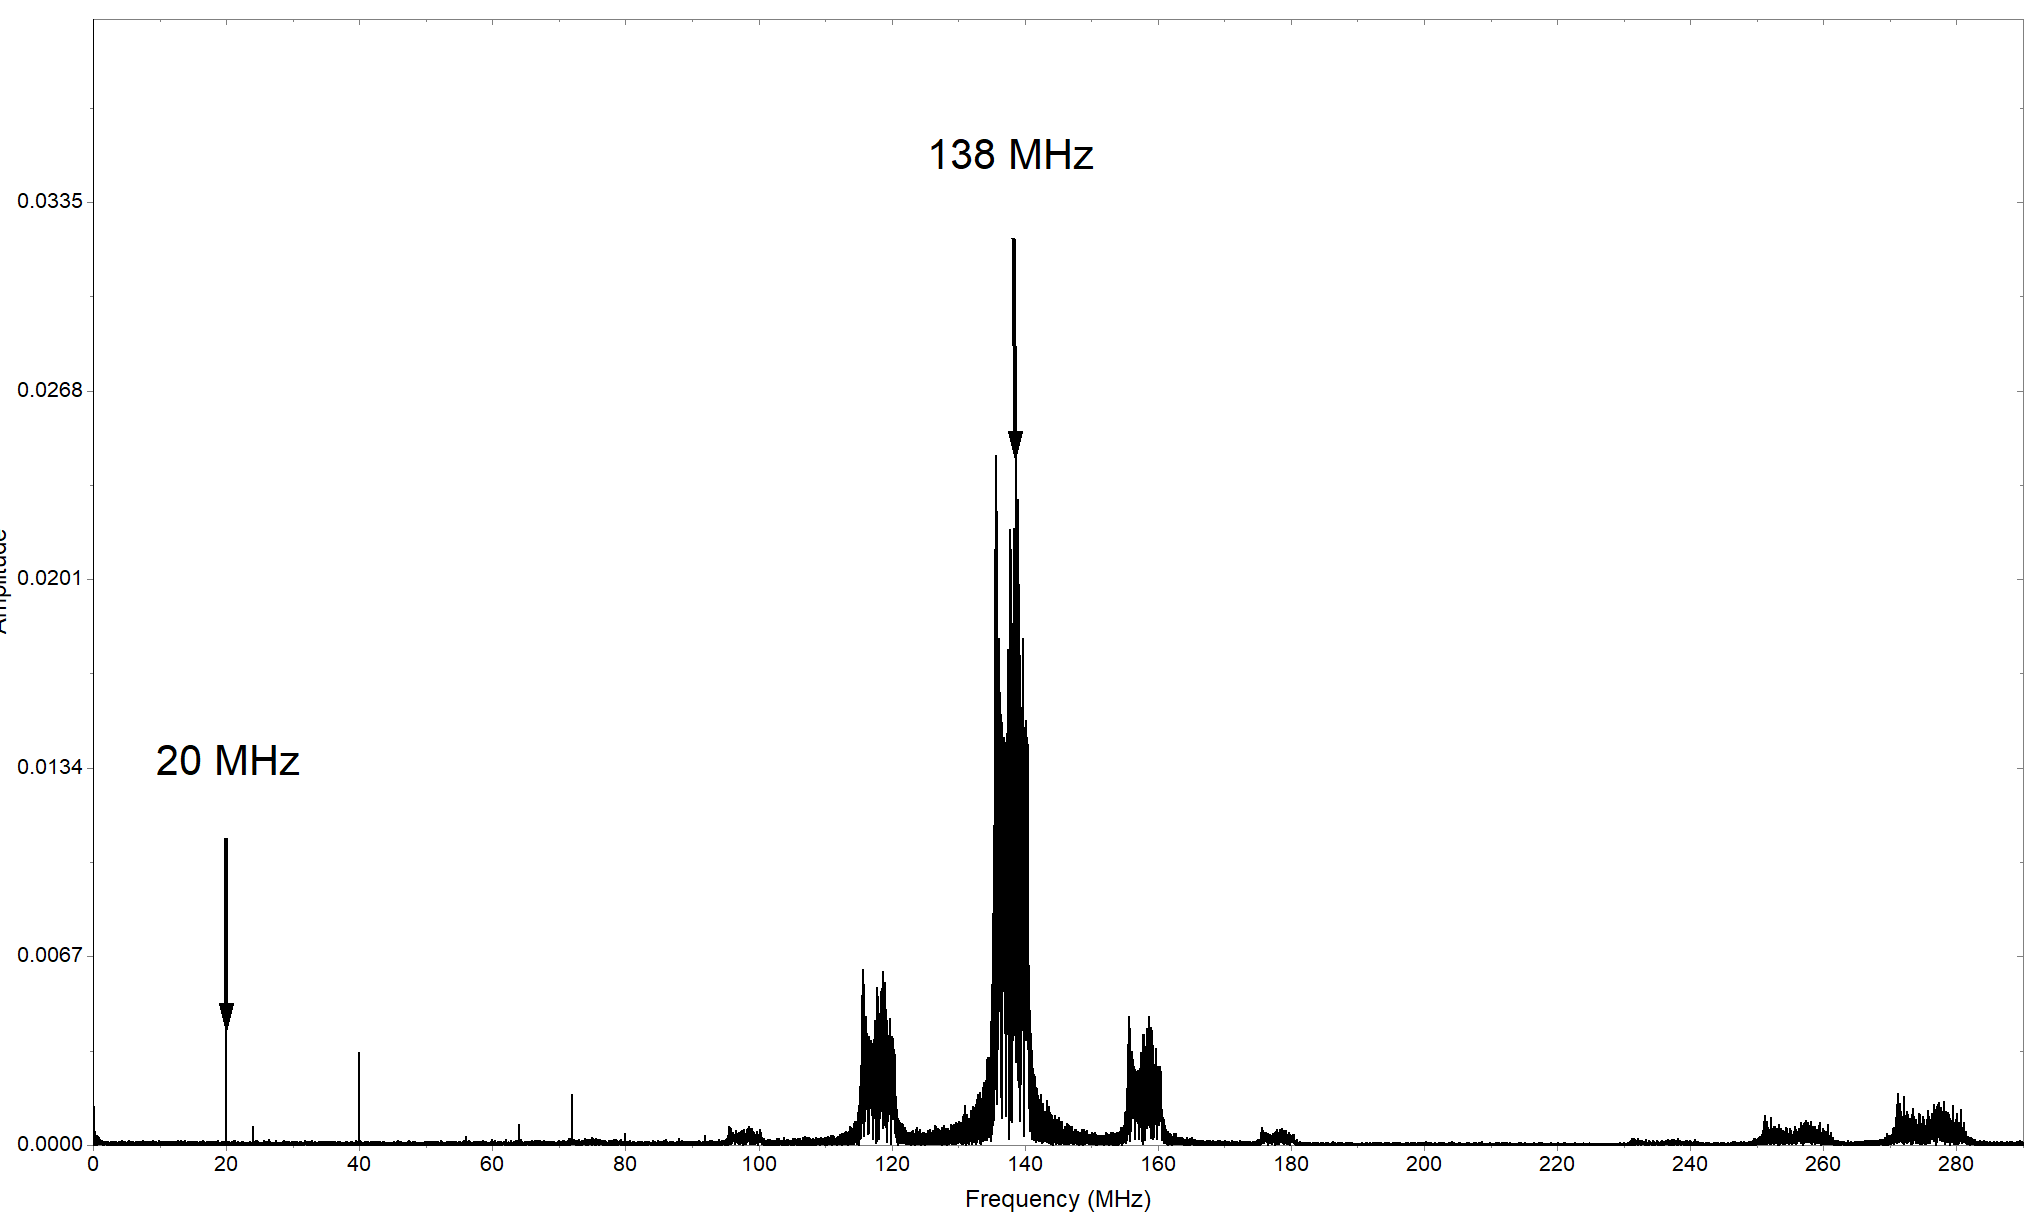
\includegraphics[width=\linewidth]{spectrum_het_true_ruin_pol.png}
    \caption{Spectrum of ruined polarisation}
    \label{fig:ruined pol syn}
\end{figure}
\begin{figure}
    \centering
    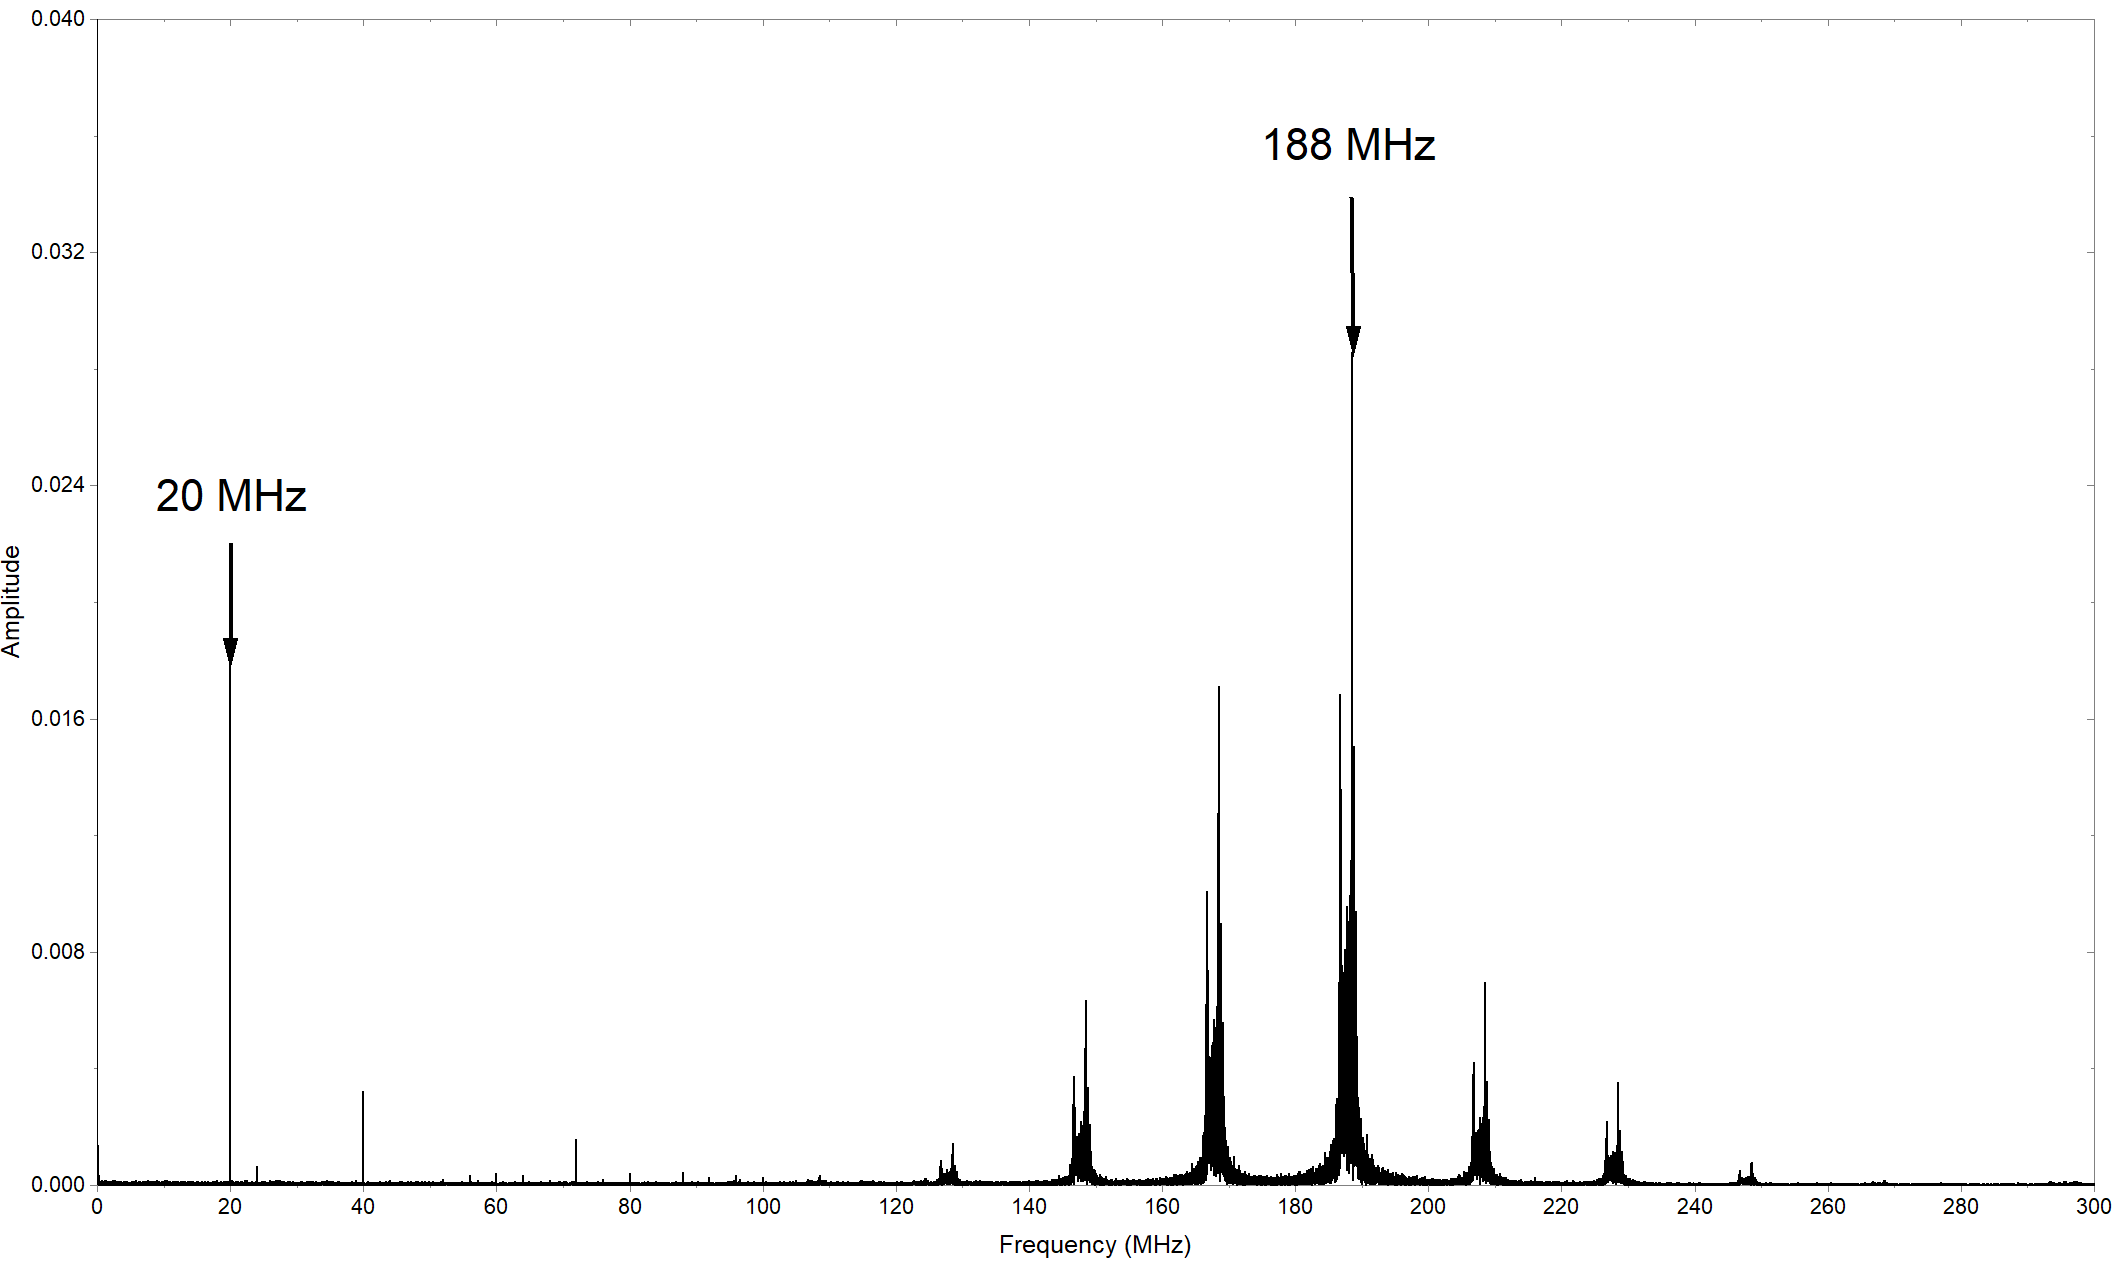
\includegraphics[width=\linewidth]{spectrum_het_true_norm_pol.png}
    \caption{Spectrum of a signal with distorted polarisation}
    \label{fig:norm pol syn}
\end{figure}
Figure~\ref{fig:ruined pol syn} shows the spectrum of an information signal with distorted polarisation. The information about the presence of a doubled modulation frequency is fed to the polarisation controller and it starts its operation until the true modulation frequency is maximal and the doubled modulation frequency disappears. The result of the algorithm is shown in Figure~\ref{fig:norm pol syn}. The spectrum of the signal at normal polarisation contains no harmonic at the doubled frequency and the harmonic at the modulation frequency is maximal.
\newline To the advantages of this method can be attributed flexibility in the choice of protocol, as the transfer of information to the intermediate frequency allows you to analyse almost any modulation without the need to introduce additional elements, for example, phase modulator to select the basis. The use of two independent sources of coherent radiation allows not to use feedback systems, which require an additional optical channel and open additional opportunities for an intruder. Generation of a local oscillator on the receiver side allows to increase its power, compared to protocols in which LO is transmitted over a quantum channel, which allows to reduce noise associated with scattering in the FOCL and increase the signal-to-noise ratio, which positively affects the bit rate.
\newline From the disadvantages of the same can be highlighted the need to adjust the frequency, as two independent oscillators need periodic frequency adjustment. This problem is solved by the peculiarity of the protocol of quantum communication at side frequencies due to the fact that in the spectrum there is a powerful carrier, which is also knocked down with the local oscillator and is transferred to an intermediate frequency. By analyzing this frequency after FFT processing, it is possible to adjust the LO frequency so that all signals fall within the bandwidth of the balanced detector. Another disadvantage is the random phase noise due to the randomness of the laser generation process in two independent sources. This problem is solved by analyzing the phase of the intermediate frequency between the local oscillator and the optical carrier obtained after Alice phase modulation. This signal will contain the phase noise of both the LO and the transmitter laser, which can be accounted for in post-processing by pre-processing with digital methods. 
\underline{Chapter Four} is devoted to the study of the effect of the intruder radiation at a wavelength of 1310 nm on the source of coherent radiation based on a semiconductor laser diode with distributed feedback. This vulnerability in its technical implementation is called optical pumping attack. This type of attack is similar to the Laser Seeding attack in that Eve injects its radiation into the laser resonator on the transmitter to alter its characteristics. However, there is a significant difference. In the case of a seeding attack, the attacker uses the same or close wavelength to the operating wavelength of the laser under attack. Whereas in the case of an optical pumping attack, Eve uses a laser wavelength that differs by 50 nanometers or more from the operating wavelength of Alice's laser. This feature makes it possible to more effectively circumvent countermeasures using passive fibre-optic elements in the form of isolators. Their isolation coefficient has a spectral dependence, which leads to the fact that the insertion isolation at 1310 nm wavelength is significantly smaller than at 1550 nm wavelength. As a result, the attacker requires less probing power to achieve the desired effect. 
\newline This attack is constructed as follows. The attacker installs a fibre circulator with three ports into the break in the fibre optic link. Eve's probing laser is plugged into the first port. The second port is plugged into the fibre optic link towards the sender side and the third port is plugged into the receiver side. In this way the intruder's radiation will enter the optical circuitry of the transmitter, and Alice's radiation will pass through the fibre towards the receiver without any problems. The intruder's radiation undergoes attenuation as it passes through the optical circuitry of the transmitter, so it is necessary to have sufficient probing power to make changes to the laser characteristics. The passed radiation enters the laser crystal and is absorbed in it.
\begin{figure}
    \centering
    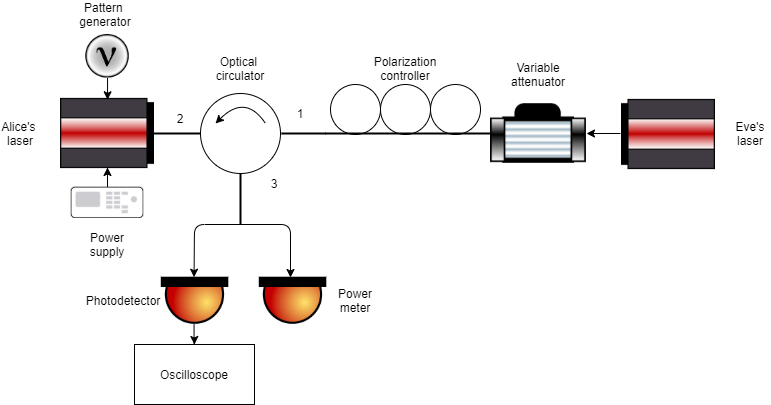
\includegraphics[width=0.75\textwidth]{images/1310 experiment.png}
    \caption{Schematic of the laser seeding experiment. Alice's Laser - Alice's Laser, Pattern generator - pulse sequence generator, Power Supply - laboratory power supply, optical circulator - optical circulator, polarisation controller - polarization controller, varriable attenuator - tunable attenuator, Eve's laser - intruder laser, Photodetector - photodetector, power meter - power meter, Oscilloscope - oscilloscope}.
\label{fig:exper 1310 syn}
\end{figure}
This causes an additional population inversion to be created, resulting in a shift in the Watt-Ampere characteristic of the laser while the pump current is unchanged.
\begin{figure}
    \centering
    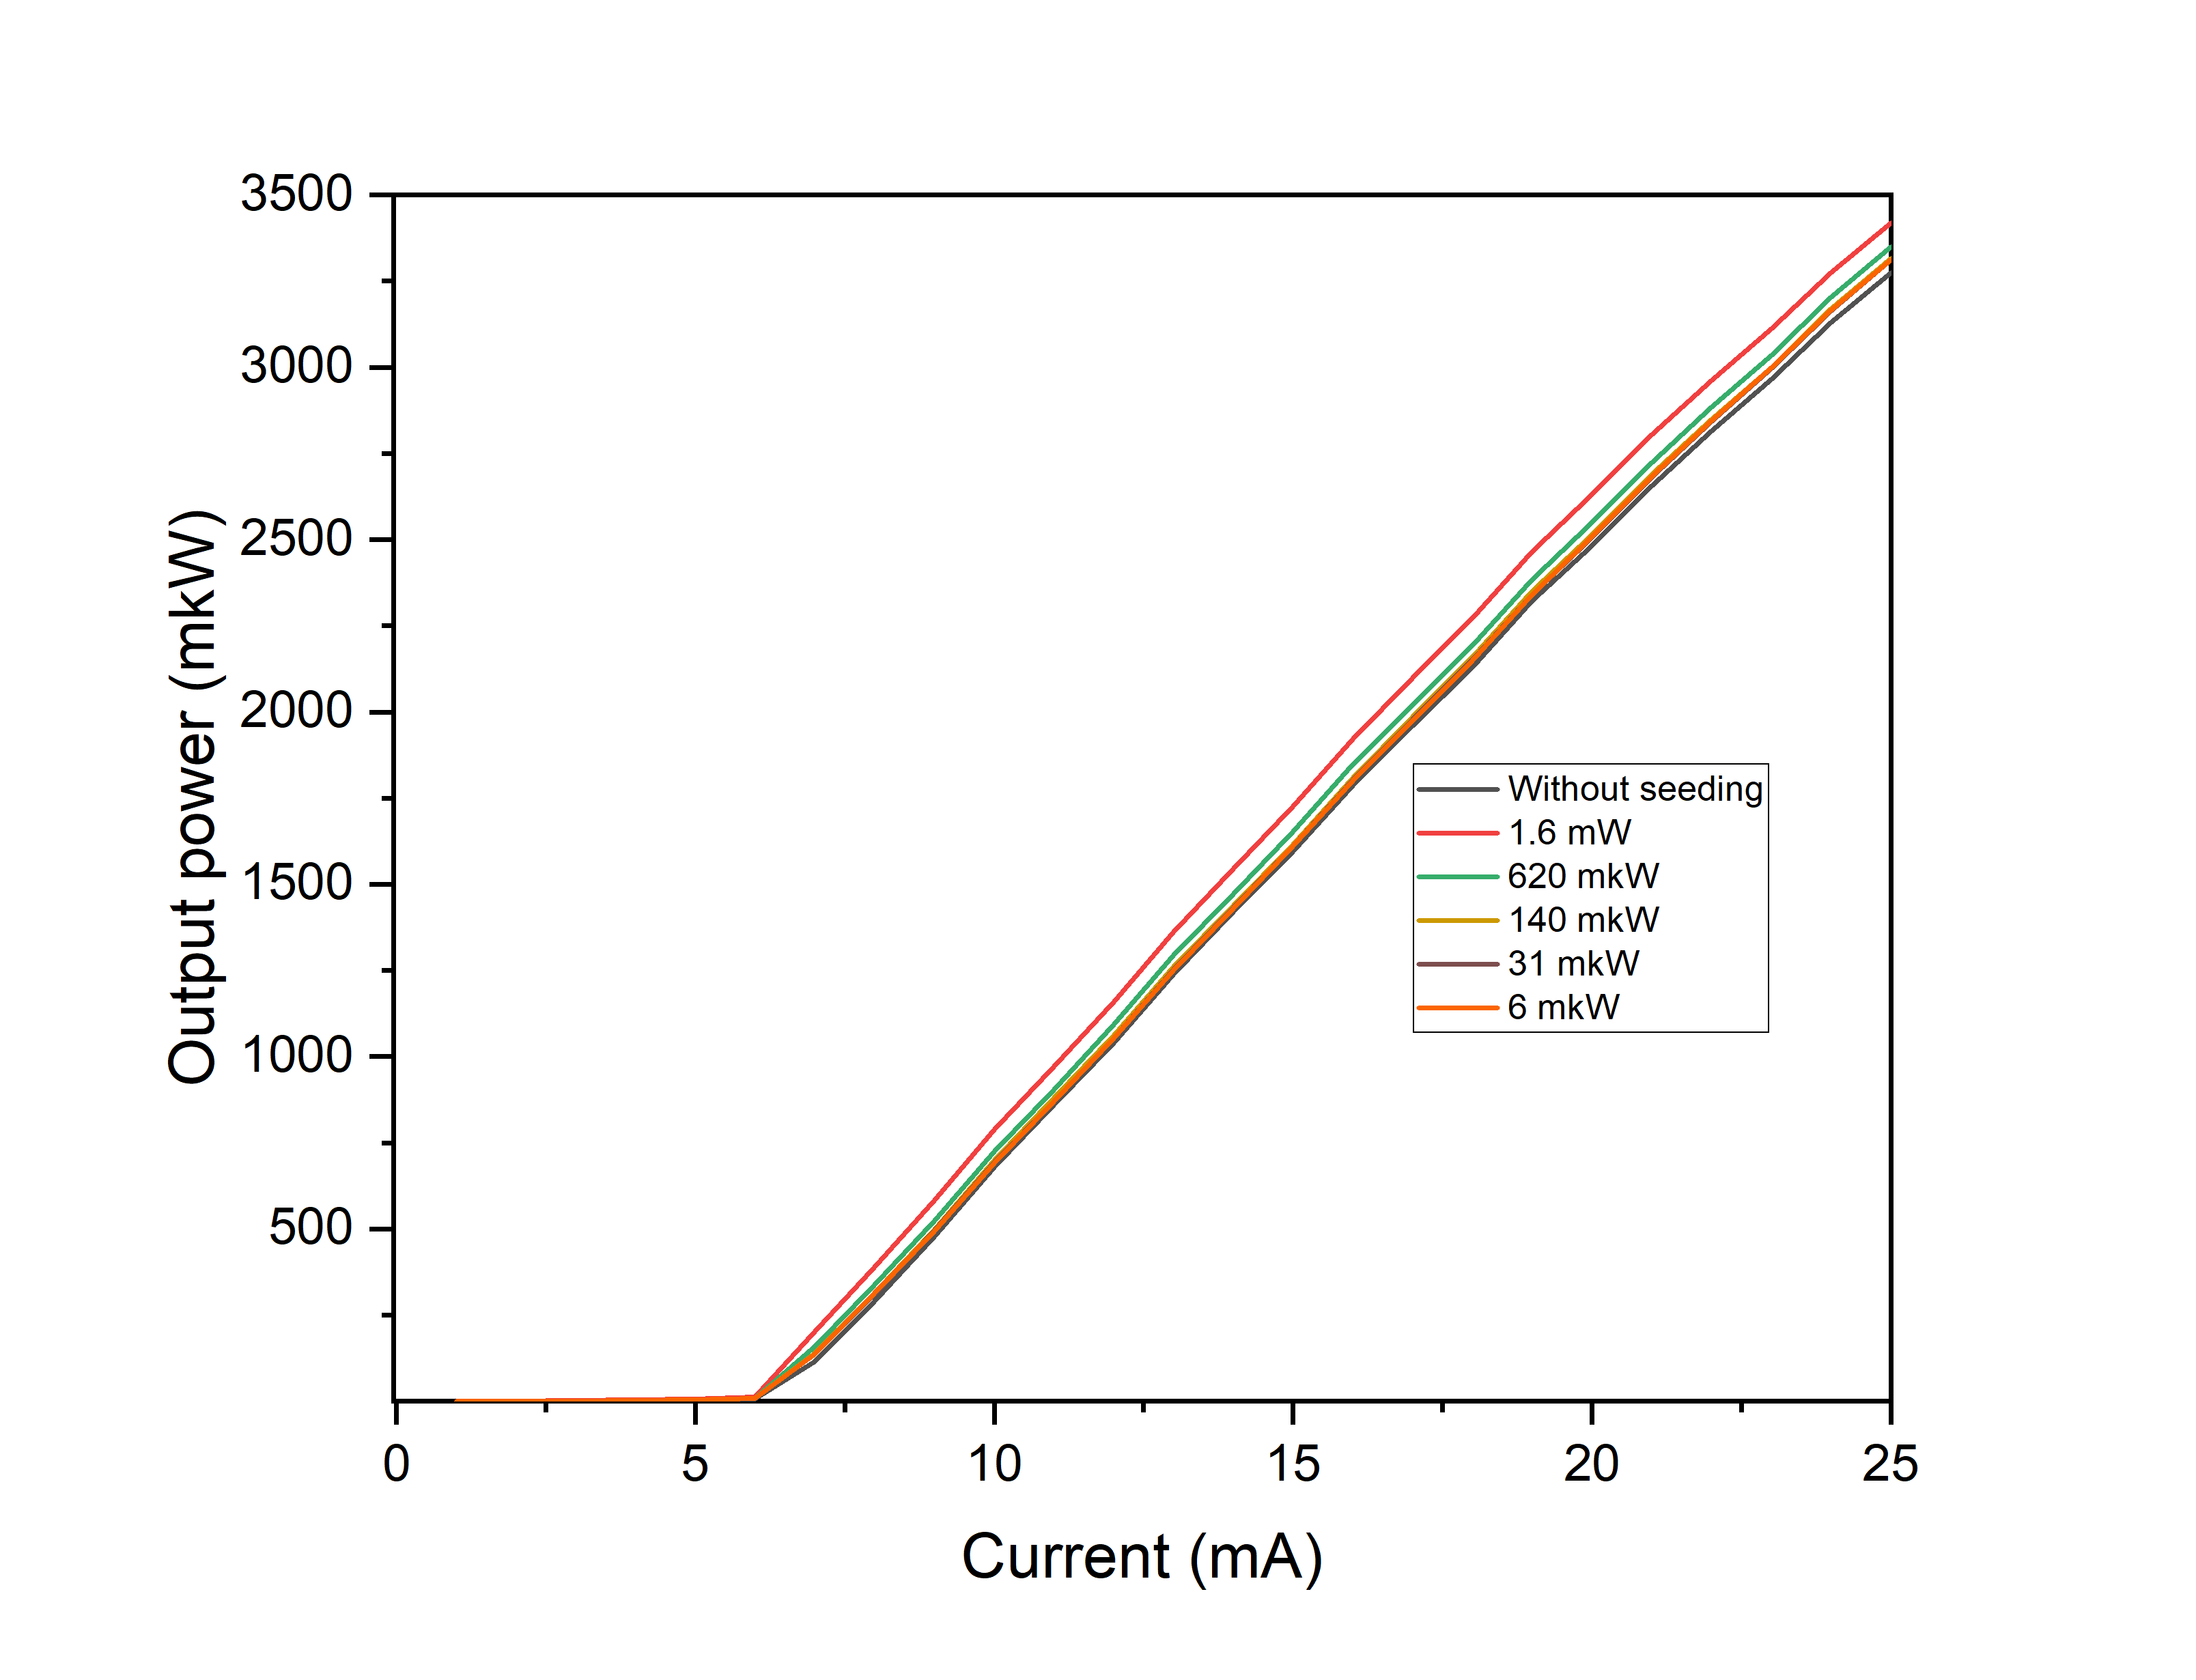
\includegraphics[width=0.75\textwidth]{images/ватт ампер для диссера.png}
    \caption{Variation of Watt Ampere characteristics under different pump powers at 1310 nm wavelength. Output power is output power in microwatts, current is current in milliamperes}
    \label{fig:watt-amp syn}
\end{figure}
This causes the calibrated radiation source on the transmitter side to start emitting more power than originally intended. As a result, this causes the output average photon number to increase, generating a larger number of multiphoton states, which opens up the possibility of realising a photon number splitting attack. The same effect is manifested in the change of the pulse shape. Optical pumping increases the pulse area and, consequently, its energy, increasing both the average number of photons in signal pulses and the average number of photons in decoy states in the BB84 protocol with decoy states.

\begin{figure}
    \centering
    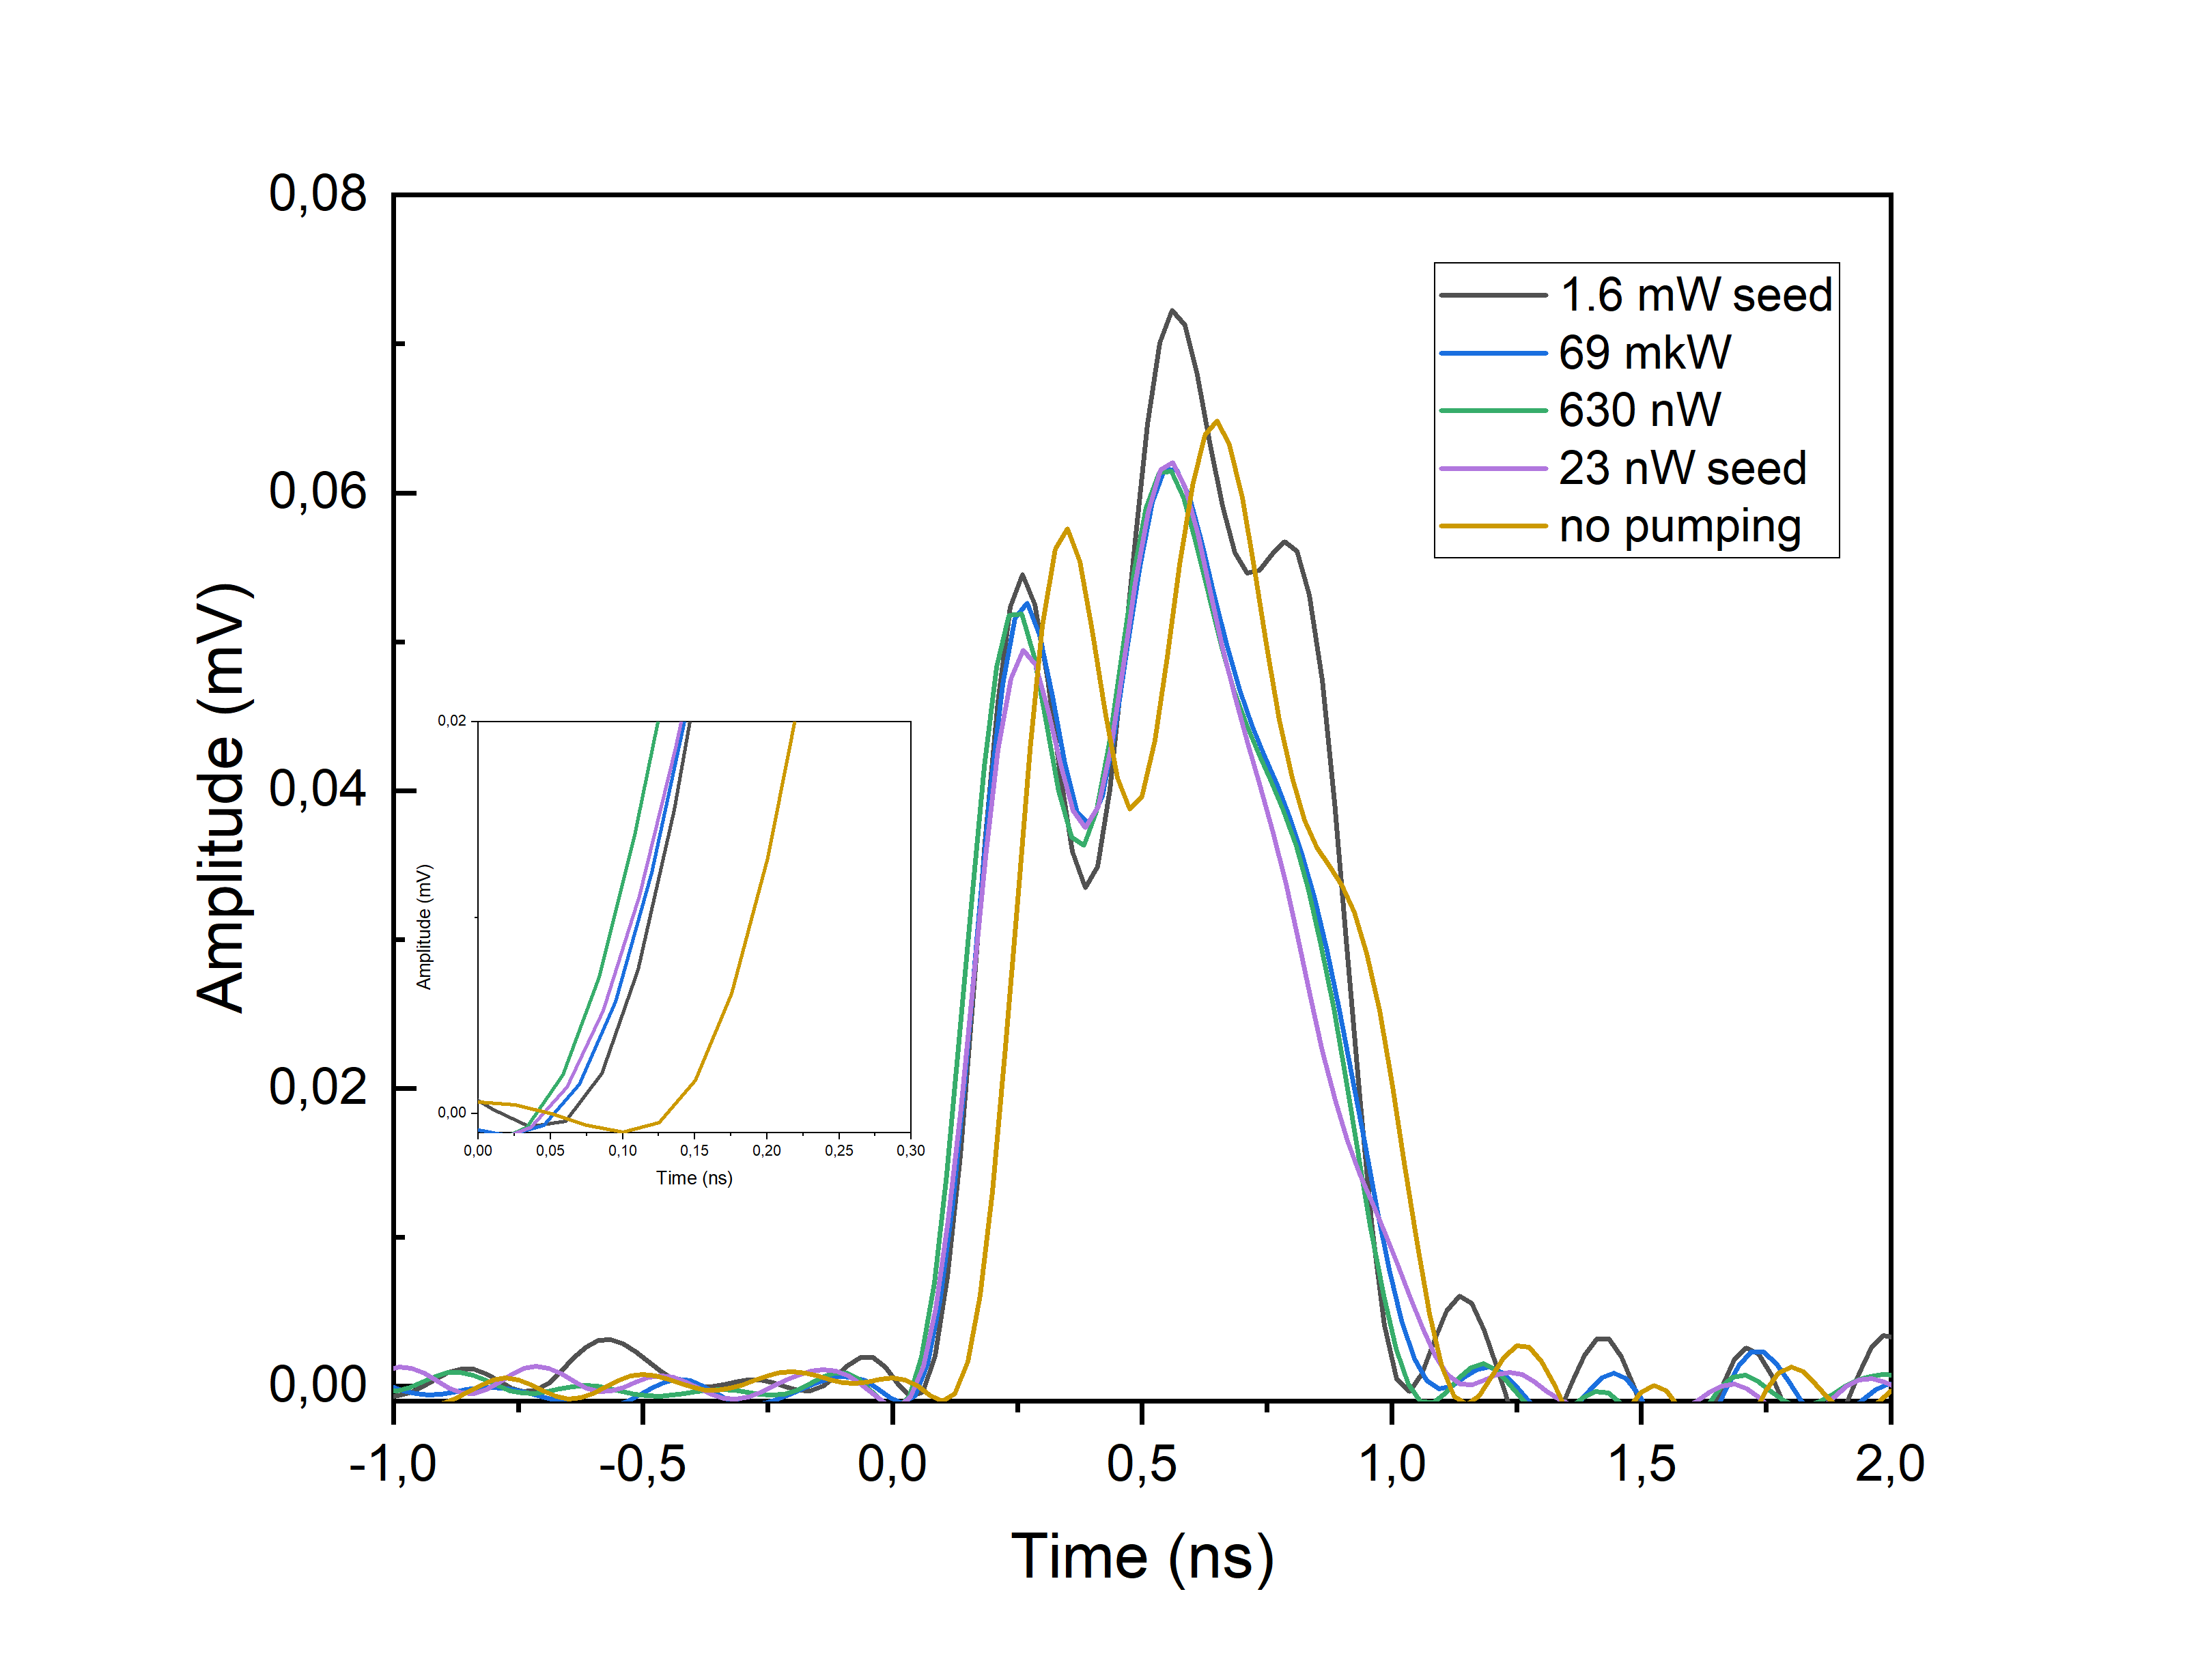
\includegraphics[width=0.75\textwidth]{images/Импульсы под действием 1310 для диссера.png}
    \caption{Change of pulse shape under the action of external optical pumping at different powers at the wavelength of 1310 nm. Amplitude is amplitude in millivolts, Time is time in nanoseconds, seed is seeding, and pumping is pumping}.
    \label{fig:pulses 1310 syn}
\end{figure}
\newpage In the framework of this work, we show the implementation of an optical pumping attack at a wavelength of 1310 nm, which leads to an increase in the laser output power at constant pump currents, an increase in the pulse area, and an increase in the quantum efficiency of the laser. These effects create conditions for other types of attacks on the QRC system. In the case of this work it was shown that a probing power of 200 $\mu W$ is sufficient to increase the quantum efficiency by 1\%, demonstrated in the graph \ref{fig:eff syn} and to increase the output power by $4\%$. The minimum power required for an attacker to effectively attack a typical optical transmitter circuit implementing the BB84 protocol was calculated.
\begin{figure}
    \centering
    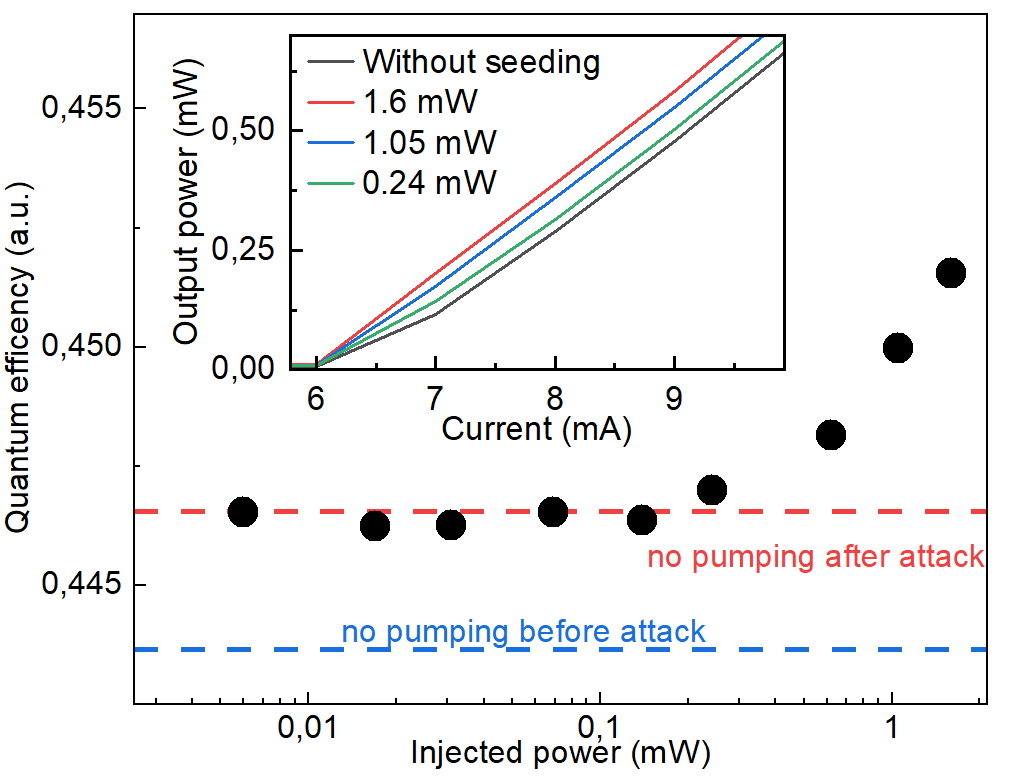
\includegraphics[width=0.7\textwidth]{images/Эффективность 1310.png}
    \caption{Change in quantum efficiency due to external radiation at 1310 nm wavelength. Quantum efficiency - quantum efficiency in relative units, Output power - output power in milliwatts, Injected power - injected power in milliwatts, current - current in milliamperes, blue dashed line - value of quantum efficiency before attack, red dashed line - value of quantum efficiency after attack. }
    \label{fig:eff syn}
\end{figure}
\newpage The research conducted in the \underline{chapter six} is devoted to the study of the effect of high-power coherent radiation on a laser source based on optical injection. Such sources are actively used in quantum communication systems implementing a protocol with an untrusted receiver node. Such sources have improved output signal amplitude stability, temporal wavelength stability, and reduced output pulse chirp by reducing the influence of transients during generation. These features allow us to obtain a Hong-Ou-Mandel interference prominence close to the theoretical maximum of 0.5. 
\newline However, for such sources have not been investigated methods of influence such as attack 'seeding' laser. For this purpose, an optical circuit was assembled to investigate the effect of high-power laser irradiation in the power range from 180 to 900 mW. 
\begin{figure}
    \centering
    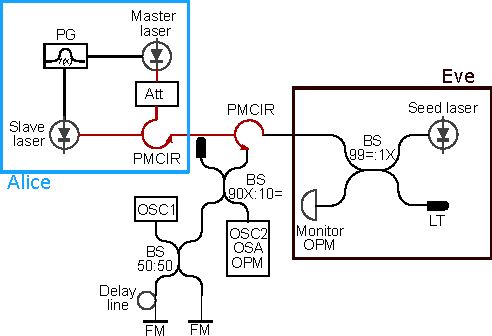
\includegraphics[width=0.9\textwidth]{images/setup_Faraday_Mirrors_final.pdf}
    \caption{Optical schematic diagram of laser source seeding setup based on optical injection}.
    \label{fig:enter-label}
\end{figure}

Two distributed feedback semiconductor lasers were assembled as the source. The first laser was an Agilecom WSLS-934010C4124-42 laser with an integrated isolator, which was used as the master laser to generate the reference radiation. The second laser, however, was an Agilecom WSLS-934010C4124-82 laser, similar to the first laser, but without an integrated insulator. This is to maximize the amount of radiation injected into the resonator of the slave laser. The two lasers are connected to each other via an optical circulator. Its first port is connected to the master laser, the radiation from which enters the second port of the circulator where the slave laser is connected. In this way, the study from the master laser enters the resonator of the slave laser. The radiation from the slave laser enters the second port of the circulator and passes to the third port of the circulator. A Gooch\& Housego AA1406-193300 laser and an erbium fiber amplifier were used as a source of high-power laser radiation. To introduce its radiation, an additional circulator was used, the first port of which was connected to the amplifier output, the second to the third port of the first circulator. A Michelson fiber interferometer was assembled to investigate the interference of the received pulses.
\newline In the course of this work, the characteristics of the output pulses under the influence of external radiation were investigated. The following parameters were studied: amplitude of output pulses and their stability expressed in the measurement of standard deviation, duration of pulses and their standard deviation, as well as the correlation of the phase of the received pulses using a fiber Michelson interferometer. During exposure, the standard deviation of the energy of the output pulses was varied between 2 and 3.5 per cent at an attack laser power of 900 mW and by varying the master laser power. The results of these measurements are shown in Figure \ref{fig:area MDI syn}
\begin{figure}
    \centering
    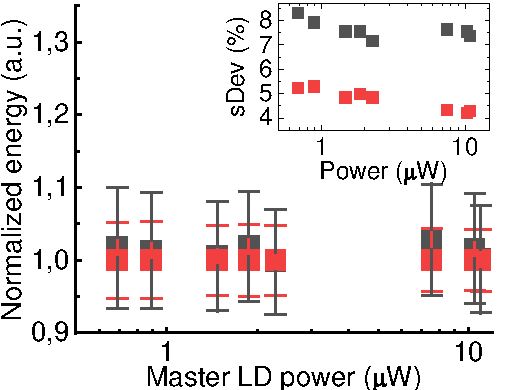
\includegraphics{images/area_under_attack.pdf}
    \caption{Change in source pulse energy with and without external radiation as a function of master laser power}.
    \label{fig:area MDI syn}
\end{figure}
These results show that Eve is able to increase the output power instability to increase the average number of photons per pulse. The pulse duration is also altered by external radiation, shown in Figure \ref{fig:duration syn} the external influence increases the pulse jitter by $2\%$.  Existing work shows that even small deviations in pulse duration significantly reduce the distribution range of the secret key. 
\begin{figure}
    \centering
    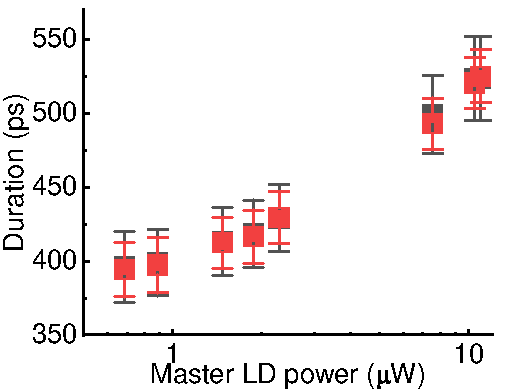
\includegraphics{images/duration_change.pdf}
    \caption{Change in pulse duration due to external radiation}
    \label{fig:duration syn}
\end{figure}
\newline To develop a countermeasure, it is necessary to calculate the necessary isolation factor for the worst case scenario, when the attacker uses the maximum available power. In continuous mode, this value is 2 watts. This value needs to be attenuated to less than -35 dBm. By using a fibre optic circulator as part of the circuit, the isolation value is already 50 dB.  To calculate the required attenuation value, the following formula is used
\begin{equation}
\label{eq:isolation syn}
    \alpha = P_a - P_{req} - \beta.
\end{equation}, where $\alpha$ is the amount of isolation to be introduced, $P_a$ is the amount of probing power in dBm, $P_{req}$ is the power to which the input radiation needs to be attenuated, $\beta$ is the amount of isolation that is already implemented in the circuit, in dB. 
Let's substitute in~\ref{eq:isolation syn} the values of 33 dBm of power, which corresponds to 2 watts of power and 50 dB of isolation. The resulting isolation value required to attenuate 2 watts to -35 dBm is 18 dB. To ensure the safety of this source, it is sufficient to install a fiber isolator with a typical isolation value of 30 dB. This will cover the entire allowable range of sensing power. 
\newline The obtained results demonstrate the resistance of the proposed source of coherent radiation to external influences. To change its characteristics, an intruder needs to operate at powers close to those that trigger a spark in fibre-optic communication lines, which carries an increased risk of being detected. And protocols based on the protocol using an untrusted receiver node are not only secure from attacks of an intruder on receiver nodes in the form of single photon detectors, but also from attacks on single photon sources.
In the \underline{conclusion} the main results and conclusions obtained during the work are presented.
The \textbf{introduction} describes the relevance of the work and formulates its goals and objectives.
\newline \textbf{Chapter} provides an overview of the current literature on quantum key distribution, its protocols, and modern attacks on its technical implementation.
\newline \textbf{Chapter} \ref{ch:ch2} presents the results of creating a quantum key distribution system at side frequencies on continuous variables using optical injection as feedback for a local oscillator. A mathematical model of the optical injection method in semiconductor lasers is provided. The problem of synchronising the wavelengths of quantum states and the local oscillator is described. Key distribution is performed experimentally using the proposed synchronisation method.
\newline \textbf{Section} \ref{sec:ch2/sect9} describes the principle of operation of the quantum key distribution system at side frequencies.
\newline \textbf{Section} \ref{sec:ch2/sect1} describes the optical injection method and its advantages. A mathematical model is provided.
\newline \textbf{Section} \ref{sec:ch2/sect2} provides a model of the frequency range in which the optical injection method can be implemented and the conditions for its occurrence.
\newline \textbf{Section} \ref{sec:ch2/sect7} describes a method for measuring the wavelength of radiation from a local oscillator under the influence of external radiation and presents the results of experimental data obtained using this method.
\newline \textbf{Section} \ref{sec:ch2/sect3} presents a mathematical model of heterodyne detection for a quantum key distribution system at side frequencies with optical injection. The results demonstrate that the signal received at the receiver side will only be observed at the modulation frequency.
\newline \textbf{Section} \ref{sec:ch2/sect4} describes the features of a quantum key distribution system at side frequencies on continuous variables using optical injection, and describes the advantages of using optical injection.
\newline \textbf{Section} \ref{sec:ch2/sect5} presents an experimental setup for a quantum key distribution system on side frequencies on continuous variables using optical injection.
\newline \textbf{Section} \ref{sec:ch2/sect6} describes the results of the experiment. It is shown that the experimental results agree with the mathematical model described in section \ref{sec:ch2/sect3}, and the possibility of extracting information about the phase of quantum states from the intermediate frequency is demonstrated.
\newline \textbf{Section} \ref{sec:ch2/sect8} presents the conclusions of the chapter.
\newline \textbf{Chapter}\ref{ch:ch3} demonstrates the experimental implementation of a quantum key distribution system at side frequencies on continuous variables with two independent radiation sources without the use of feedback. The method of heterodyne signal reception and the protocol for forming a bit sequence for the described system are described.  A mathematical model of heterodyne signal detection for a quantum key distribution system at side frequencies with independent radiation sources is presented. A description of the experimental setup and experimental results is provided. The polarisation control algorithm is described and its effect is demonstrated.
\newline \textbf{Section} \ref{sec:ch3/sect1} describes the heterodyne detection method and its advantages for a quantum key distribution system at side frequencies.
\newline \textbf{Section} \ref{sec:ch3/sect2} describes the protocol for quantum key distribution at side frequencies using the heterodyne signal detection method.
\newline \textbf{Section} \ref{sec:ch3/sect3} describes the optical scheme of an experiment to implement heterodyne signal detection for a sideband quantum key distribution system on continuous variables with two independent radiation sources.
\newline \textbf{Section} \ref{sec:ch3/sect4} presents a mathematical model of heterodyne detection for the described system. The result is a signal at an intermediate frequency that coincides with the modulation frequency and carries information about the quantum state transmitted by Alice.
\newline \textbf{Section} \ref{sec:ch3/sect5} describes the operation of the polarisation control algorithm for a quantum key distribution system at side frequencies on continuous variables with two independent radiation sources. It has been experimentally shown that polarisation distortions lead to a reduction in the number of spectral components in the output signal of the balanced detector, and the possibility of adjusting the polarisation based on the results of the Fast Fourier Transform applied to this signal has also been demonstrated.
\newline \textbf{Section} \ref{sec:ch3/sect6} describes the experimental setup, its components, and how they work.
\newline \textbf{Section} \ref{sec:ch3/sect7} describes and analyses the experimental results. It is shown that the information about the quantum states encoded by Alice is contained in the envelope of the signal at the output of the balanced detector, which is transmitted at the modulation frequency.
\newline \textbf{Section} \ref{sec:ch3/sect8} presents the conclusions of the chapter.
\newline \textbf{Chapter}\ref{ch:ch4} describes a new type of attack on a radiation source in the form of a distributed feedback laser (DFB-laser). An increase in the average output power and energy of pulses emitted by the laser under attack is experimentally demonstrated, with the current and pump pulse parameters remaining unchanged. The existing quantum key distribution system is analysed for resistance to this type of attack, and the minimum power required to carry out the attack is determined, as well as the necessary isolation to protect against it.
\newline \textbf{Section} \ref{sec:ch4/sect1} describes the principle of the attack and compares it with an existing attack on an optical radiation source. A description of the experimental setup and its principle of operation is provided.
\newline \textbf{Section} \ref{sec:ch4/sect3} presents measurements of the watt-ampere characteristics of the laser under the action of an 'optical pumping' attack at different attacker power levels. The differential quantum efficiency is calculated.
\newline \textbf{Section} \ref{sec:ch4/sect4} describes the experimental results of measuring the dependence of the average power and energy of pulses emitted by a laser in a KRK system under the influence of different attacker pump powers.
\newline \textbf{Section} \ref{sec:ch4/sect5}, the minimum isolation required to prevent an attack is calculated based on experimental data and information from the literature.
\newline \textbf{section} \ref{sec:ch4/sect6}, the resistance of the quantum key distribution system is calculated from the open literature and its resistance to this type of attack is assessed.
\newline \textbf{section} \ref{sec:ch4/sect7}, conclusions on the chapter are presented.
\newline \textbf{Chapter}\ref{ch:ch5} is devoted to the study of the 'seeding' attack on a radiation source based on optical injection. A mathematical model of optical injection is described. A comparison of the characteristics of laser sources with and without optical injection is carried out. The experimental setup is described. The dependence of the output power and pulse characteristics on the ratio of the powers of the attacked and driving lasers is investigated. The dependence of the attack on the wavelength of the attacker's radiation source is described.
\newline \textbf{Section} \ref{ch:ch5/sect1} motivates the need for the research conducted in this work.
\newline \textbf{Section} \ref{ch:ch5/sect2} describes a mathematical model of a radiation source with optical injection. A comparison of the interference pattern of a pulsed laser source with and without optical injection is provided, and the visibility of the interference pattern is calculated.
\newline \textbf{Section} \ref{ch:ch5/sect3} provides a diagram of the experimental setup and describes the radiation source under study based on optical injection. The parameters of the laser radiation under study are described.
\newline \textbf{Section} \ref{ch:ch5/sect4} describes the experimental results. It is shown that external radiation from an attacker increases the average radiated power of the optical injection-based radiation source. An increase in pulse energy and the invariance of temporal characteristics are shown, and interference patterns under attack are investigated. The dependence of the attack on the wavelength of the attacker's seeding is also described.
\newline \textbf{Section} \ref{ch:ch5/sect5} presents the conclusions of the chapter.
\newline \textbf {Conclusion} contains all of describes all the main results of the work.
\section*{Publications on the topic of the dissertation}

Publications in international journals indexed by Scopus:\\
\begin{enumerate}
    \item Goncharov R.K.,\underline{Fadeev M.A.}, Zinovev A.V., Nasedkin B.A., Kiselev A., Egorov V.I. Coherent detection schemes for subcarrier wave continuous variable quantum key distribution // Journal of the Optical Society of America B: Optical Physics -- 2021, Vol. 38, No. 6
    \item Pervushin B.E., \underline{Fadeev M.A.}, Zinovev A.V., Goncharov R.K., Santev A.A., Ivanova A.E., Samsonov E.O. Quantum random number generator using vacuum fluctuations // Наносистемы: Физика, химия, математика = Nanosystems: Physics, Chemistry, Mathematics - 2021, Vol. 12, No. 2, pp. 156--160
    \item \underline{Fadeev M.A.}, Goncharov R., Smirnov S., Chistiakov V. Continuous variable measurement-device-independent quantum communication scheme based on subcarrier waves // Proceedings - International Conference Laser Optics 2022, ICLO 2022
    \item Boltanskii M.V., Maksimova E.I., \underline{Fadeev M.A.}, Shakhovoy R.A. Influence of optical feedback on an optical pulse shape of a semiconductor laser // Научно-технические ведомости Санкт-Петербургского государственного политехнического университета. Физико-математические науки = St.Petersburg State Polytechnical University Journal. Physics and Mathematics, 2024, Vol. 17, No. 3.1, pp. 224--228
    \item Latypov I.Z., Chistyakov V.V., \underline{Fadeev M.A.}, Sulimov D.V., Khalturinsky A.K., Kynev S.M., Egorov V.I. Hybrid quantum communication protocol for fiber and atmosphere channel // Наносистемы: Физика, химия, математика = Nanosystems: Physics, Chemistry, Mathematics, 2024, Vol. 15, No. 5, pp. 654 -- 657
    \item \underline{Fadeev M.A.}, Ponosova A.A., Huang A., Shakhovoy R., Makarov V. Secure laser source for QKD systems // Proceedings - International Conference Laser Optics 2024, ICLO 2024, 2024, pp. 571
    \item \underline{Fadeev M.A.}, Ponosova A.A., Shakhovoy R., Makarov V. Laser-pumping attack on QKD sources // Proceedings - International Conference Laser Optics 2024, ICLO 2024, 2024, pp. 562
\item \underline{Fadeev M.A.}, Morozova P.A., Smirnov S.V., Ivanova A.E., Kynev S.M., Chistyakov V.V., Heterodyne detection for a quantum key distribution system at side frequencies // News of higher educational institutions. Radiophysics, 2024. Volume 67, Issue 9, pp. 784--792    \item \underline{M. A. Fadeev}, A.Ponosova, Q.Peng, H.Anqi, R. Shakhovoy, and V.Makarov, `Optical-pumping attack on a quantum key distribution laser source', Opt. Express, 2025.

\end{enumerate}
Publications considered equivalent to peer-reviewed scientific publications:

\begin{enumerate}

\item Patent: "Device for Quantum Broadcast of a Symmetrical Bit Sequence on a Subcarrier Frequency of Modulated Radiation with a Double Homodyne Reception Method," patent number 2020130398.
\item Patent: "Device for Quantum Broadcast of a Symmetrical Bit Sequence on a Subcarrier Frequency of Modulated Radiation with a Homodyne Reception Method," patent number 2020130399.
\item Patent: "Device for Quantum Broadcast of a Symmetrical Bit Sequence on a Subcarrier Frequency of Modulated Radiation with a Heterodyne Reception Method," patent number 2020130400.
\item Patent: "Device for Quantum Communication on Sidebands with an Increased Degree of Information Security from External Attacks" patent number 044749.

\end{enumerate}

             % Synopsis
\chapter*{Введение}                         % Заголовок
\addcontentsline{toc}{chapter}{Введение}
\noindent 
\section*{Актуальность темы}
Квантовое распределения ключа (КРК) - актуальная технология, появившаяся из теории квантовой информатики, позволяющая распределить симметричную битовую последовательность с помощью квантовых методов у двух и более пользователей для использования этой последовательности в качестве ключа для симметричного шифрования данных и одновременным обнаружением несанкционированного доступа со стороны нелегитимных пользователей. Использование квантовых состояний света при распределении ключа позволяет достичь уровня секретности, недоступного для классических протоколов шифрования. Такие квантовые состояния могут быть представлены в виде одиночных фотонов. Их квантовые свойства не позволяют злоумышленнику скопировать их состояния или считать их без изменения и без внесения ошибок. Такие квантовые состояния возможно передавать как по волоконно-оптическим линиям связи (ВОЛС), как по атмосферным каналам, так и в космическом пространстве с помощью спутников. Принцип работы данных систем следующий. На стороне передатчика (Алиса) формируются квантовые состояния. Для этого используется когерентное лазерное излучение, ослабленное до одиночных фотонов с помощью аттенюатора. В подготовленные кванты света вносится изменение в поляризацию или фазовый сдвиг фотона. Подготовленное таким образом состояние передается по каналу связи к приемнику (Боб). На приемной стороне происходит независимое от Алисы повторное измерение состояния фотона. В случае корреляции у Боба принятый одиночный фотон регистрируется детектором одиночных фотонов. Благодаря свойствам одиночного фотона в виде невозможности клонирования, невозможности измерения без разрушения и его неделимости возможно отследить воздействие злоумышленника, так как его действия будут приводить к появлению ошибок в полученной битовой последовательности. Так обеспечивается контроль несанкционированного допуска. 

Отдельным классом выделяются системы квантового распределения ключа на непрерывных переменных (КРК-НП). В таких системах квантовое состояние, подготовленное и переданное Алисой, на приемной стороне взаимодействует с сильным лазерным излучением. И результат этого взаимодействия регистрируется балансным детектором. Основными отличиями данного детектора от детектора одиночных фотонов является использование двух классических фотоприемников, подключенных таким образом, что их фототоки взаимно вычитаются, что позволяет уменьшить шум системы, и отсутствие охлаждения до температур порядка -40$^{\circ}$  градусов Цельсия. Все это позволяет упростить конечную систему. К преимуществам КРК-НП можно отнести большую скорость выработки секретного ключа по сравнению с системами КРК на дискретных переменных, в которых применяются детекторы одиночных фотонов. 

Среди сложностей систем КРК-НП выделяется способ передачи сильного лазерного излучения или локального осциллятора (ЛО) на приемную сторону и его разделения с квантовым сигналом. В первых системах КРК-НП с Гауссовой модуляцией Локальный осциллятор и квантовые состояния генерировались у передатчика, объединялись и передавались совместно в квантовый канал. На приемной стороне локальный осциллятор и квантовый сигнал разделяются, ЛО задерживается специальной линией задержки и снова соединяются на светоделителе для взаимодействия. Результатом этого взаимодействия является интерференционная картина, распределение интенсивности которой зависит от закодированного Алисой состояния. Полученное поле регистрируется балансным детектором, на выходе такого формируется уровень напряжения, который в дальнейшем подвергается пост-обработке.  Передача локального осциллятора через канал ограничивает дальность работы системы такого типа и ограничивает скорость выработки ключа, так как для лучшей работы системы необходим ЛО как можно большей мощности. Второй проблемой является возможности злоумышленника манипулировать локальным осциллятором для создания каналов утечки информации. В качестве альтернативы предлагается использовать локальный осциллятор, сгенерированный на приемной стороне. Такое решение позволит увеличить дальность передачи ключа, скорость его выработки и закрыть уязвимость к атаке на ЛО.


Одним из перспективных подходов к реализации систем квантовой коммуникации на непрерывных переменных является система квантовой коммуникации на боковых частотах модулированного излучения. В основе данного метода лежит вынесение квантового канала на боковые частоты, которые появляются в результате модуляции оптического излучения переменным электрическим полем. Благодаря этому повышается устойчивость передаваемого сигнала ко внешним воздействиям и обеспечивается высокая спектральная эффективность, а также обеспечивается показатели по отношению скорости выработки ключа к дальности между блоками приемника и передатчика, сравнимые с другими системами квантовой коммуникации. Данный метод подходит и для реализации протоколов на непрерывных переменных с когерентными методами детектирования. В частности, в данной работе рассматривается гетеродинный метод, при котором квантовые состояния, подготовленные Алисой, передаются по волоконной линии связи к приемнику, в нем попадают на светоделитель с формулой 2х2 и коэффициентом деления 50:50 и смешиваются на нем с мощным локальным осциллятором, который отстроен по частоте от передающего лазера на величину, которая превышает частоту смены состояний. Результат интерференции регистрируется балансным детектором. На выходе балансного детектора формируется сигнал на промежуточной частоте от всего спектра сигнала, переданного Алисой. Для извлечения информации требуется провести фильтрацию с помощью фильтра низких частот и демодуляцию полученного сигнала для генерации сырого ключа. 

Одной из проблем при реализации гетеродинного метода детектирования для распределения ключа является необходимость компенсации фазовых шумов. Для этого применяют различные методы. Первым из таких методов является передача "пилотного" импульса, при детектировании которого измеряется фазовый шум, внесенный каналом. После этого измеренное значение учитывается в постобработке состояний. Второе - это реализация обратной связи в различных формах. В рамках данной работы предлагается использовать метод оптической обратной связи для системы квантового распределения ключа на боковых частотах на непрерывных переменных. Суть данного метода заключается в инжекции лазерного излучения от ведущего лазера, который является лазером передатчика, в лазер ведомый, который используется в качестве локального осциллятора в приемнике. Данный метод позволяет стабилизировать длину волны ЛО и уменьшить фазовые шумы из-за того, что оба источника являются генераторами когерентного излучения со случайной фазой.

Метод оптической инжекции требует дополнительного канала для передачи создания обратной связи. Такой канал усложняет систему и повышает требования к волоконно-оптической линии связи (ВОЛС), что особенно критично в городских линиях связи, где выделение дополнительного волокна или канала в сетях с мультиплексированием затруднительно. Решением данной проблемы может является система квантового распределения ключа на непрерывных переменных с применением гетеродинного детектирования с независимым ЛО. Суть данной системы заключается в том, что на приемнике и передатчике установлены лазеры со стабилизацией длины волны и со шириной спектральной линии менее 10 кГц. Такой подход позволяет не прибегать к постоянной подстройке длин волн лазеров и уменьшить фазовый шум, связанный с независимостью источников излучения.
Однако, фазовый шум при этом не исчезает, поэтому его все еще необходимо компенсировать. В случае реализации такого метода детектирования сигналов для протокола квантового распределения ключа на боковых частотах для этого можно использовать несущую частоту, измеряя ее фазу и внося корректировки в постобработке. 

Отличия реальных систем КРК от моделей, используемых для теоретических доказательств, могут быть использованы злоумышленником для проведения различных типов атак на оборудование, входящее в состав системы. В работах ранее было показано, что источники лазерного излучения на основе полупроводниковых кристаллов могут быть уязвимы к "засеву" внешним излучением злоумышленника на длине волны близкой к той, что использует передатчик. В результате этой атаки изменяется форма излучаемого импульса и увеличивается выходная мощность, в отдельных случаях можно наблюдать и изменение длины волны. Эти эффекты приводят к увеличению среднего числа фотонов, излучаемых передатчиком, что открывает возможность для злоумышленника атаки с расщеплением числа фотонов. 

Однако в литературе не рассматривались атака "засевом" лазерным излучением на других длинах волн. Атака такого типа опаснее тем, что для защиты от нее используются пассивные волоконно-оптические элементы, вносящие дополнительное затухание, например, изоляторы или DWDM фильтры. Но существуют работы, которые демонстрируют, что величина затухания в таких элементах может уменьшаться при существенном изменении падающей длины волны излучения. Например, изолятор с рабочей длиной волны 1550 нм вносит 50 дБ потерь при обратном прохождении, когда при облучении излучением на длине волны 1310 нм эта величина составляет 20 дБ. А в случае с DWDM фильтром, он практически не вносит затухание на длине волны 1310 нм. Таким образом, злоумышленнику гораздо проще осуществить атаку "засевом" лазерным излучением, так как на данной длине волны вносимое затухание меньше. 

Такой тип атаки носит название "атака оптической накачкой". Ее суть заключается в том, что злоумышленник зондирует лазер длиной волны, отличной от рабочей. При этом это излучение поглощается активной средой лазера передатчика так, что поглощенное излучение выступает в роли оптической накачки, которая работает как дополнение к электрической накачки полупроводникового лазера. В этом случае изменяется Ватт-Амперная характеристика лазера и его квантовая эффективность. Это приводит к тому, что изменяется энергия излученных импульсов увеличивается при неизменной величине тока накачки. В рамках данной работы впервые обозначен данный тип атаки, определена нижняя граница необходимой мощности излучения на длине волны 1310 нм для изменения характеристик изучаемого лазера и измерено влияние оптической накачки на характеристики лазера. 

В системах квантового распределения применяются источники лазерного излучения на основе оптической инжекции. Такие источники построены следующим образом: применяются два лазера - ведущий и ведомый, соединенных циркуляторном. Излучение ведомого лазера позволяет снизить дрожание излучаемых импульсов, стабилизировать мощность выходного излучения и сузить спектральную линию. Однако такие источники не исследовались на устойчивость ко внешнему излучению. Ранее показанные работы по лазерному "засеву" были проведены только для одиночных источников излучения. Источник, построенный на основе оптической инжекции, имеет несколько преимуществ относительного одиночного: наличие изоляции от квантового канала за счет оптического циркулятора и наличие внешнего излучения ведущего лазера. В рамках данной работы изучается влияние мощного лазерного излучения на длительность, дрожание и амплитуду излучаемых импульсов, продемонстрирована нижняя граница мощности излучения необходимого  для внесения изменений в работу данной системы.
\section*{Цель работы}
Разработать систему гетеродинного приема сигналов в квантовой системе коммуникаций на боковых частотах с локальным осциллятором на стороне получателя с применением оптической инжекции и исследовать устойчивость к атакам на техническую реализацию источников лазерного излучения в этой системе. 

\section*{Задачи работы}
\textbf{Задача 1}\\
Реализация обратной связи в виде оптической инжекции для системы КРК на боковых частотах с гетеродинным методом детектирования и применением непрерывных переменных. 

\textbf{Задача 2}\\
Применение гетеродинного приема сигналов в системах КРК, и гетеродинное детектирование мультиплексированного сигнала на одной несущей\\

\textbf{Задача 3}\\
Исследовать атаку оптической накачкой на источники излучения, которые могут являться локальным осциллятором для систем квантового распределения ключа на непрерывных переменных\\

\textbf{Задача 4}\\
Исследовать влияние мощного оптического излучения на источник излучения на основе оптической инжекции\\

\section*{Научная новизна}
Впервые реализована система обратной связи с помощью оптической инжекции для системы квантового распределения ключей на боковых частотах и передан просеянный ключ. Реализован гетеродинный метод детектирования сигналов с двумя независимыми источниками излучения для системы квантового распределения ключей на боковых частотах и разработан алгоритм контроля поляризации для этой системы. Впервые продемонстрирован новый тип атаки на техническую реализацию - атака оптической накачкой на источник излучения в системах квантового распределения ключей, которая позволяет увеличить излучаемое среднее число фотонов в обход существующих методов защиты. Определено экспериментально влияние мощного лазерного излучения на источник когерентного излучения на основе оптической инжекции, увеличивающее энергию излучаемых импульсов и ее разброс, увеличивает выходную мощность атакуемого источника, что в совокупности приводит к снижению скорости выработки секретного ключа.
\section*{Теоретическая и практическая значимость}
Теоретическая значимость работы определяется тем, что в рамках  ее  были переданы фазово-кодированные состояния в системе квантового распределения ключей на боковых частотах на непрерывных переменных с гетеродинным методом детектирования сигналов и были стабилизированы длины волн информационного лазера и лазера локального осциллятора. Также в рамках работы был совершен обмен фазово-кодированными состояниями в системе квантового распределения ключей на боковых частотах на непрерывных переменных с гетеродинным методом детектирования сигналов и двумя независимыми источниками излучения информационного сигнала и локального осциллятора, в рамках передачи таких состояний отработан алгоритм подстройки поляризации информационного излучения. Увеличена выходная средняя мощность и энергия импульсов лазера с распределенной обратной связью, используемого в системах квантового распределения ключей, с помощью оптической накачки на длине волны 1310 нм. Увеличена средняя выходная мощность и среднеквадратическое отклонение амплитуды выходных импульсов, излучаемых источником когерентного излучения на основе оптической инжекции, с помощью мощного лазерного излучения злоумышленника, приводящее к созданию дополнительной уязвимости по доступу к секретному ключу. 
Практическая значимость работы заключается в том, что проведенные экспериментальные исследования по реализации гетеродинного метода детектирования сигналов показывают работоспособность данного подхода для создания систем квантового распределения ключей с применением такого способа регистрации сигналов. Исследованные же методы воздействия злоумышленника на источники излучения в системах квантового распределения ключей позволяет усовершенствовать модель нарушителя, повысив устойчивость конечных систем квантового распределения ключей к атакам на техническую реализацию. 

\section*{Основные положения, выносимые на защиту}
\begin{enumerate}
    \item Передача фазово-кодированных сигналов в системе квантового распределения ключей на непрерывных переменных с гетеродинным методом детектирования сигналов и локальным осциллятором, реализованным на стороне приемника, становится возможной при стабилизации длин волн используемых источников излучения за счет применения метода оптической инжекции для реализации обратной связи.
    \item Алгоритм, заключающийся в контроле поляризации входящего сигнала,  основанный на анализе спектрального состава электрического сигнала, полученного после Быстрого Преобразования Фурье, и с поворотом поляризации на основе проведенного анализа, позволяет произвести обмен фазово-кодированными состояниями в системе квантовой коммуникации на боковых частотах с применением непрерывных переменных и гетеродинным методом регистрации сигналов на основе двух независимых источников лазерного  излучения телекоммуникационного диапазона длин волн  и с применением частотного мультиплексирования на одной несущей частоте. 
    \item Поглощение излучения лазера нарушителя  активной средой полупроводникового лазера с распределенной обратной связью, используемого в передатчике системы квантового распределения ключей, приводит к увеличению излучаемого им среднего числа фотонов.
    \item Засеивание ведомого лазера в источнике излучения, построенного  на основе метода оптической инжекции, лазером нарушителя, который работает в непрерывном режиме, мощностью не менее 800 мВт и на длине волны, согласованной с длиной волны ведомого лазера,  повышает стандартное отклонение амплитуды выходных импульсов ведомого лазера на $3\%$, повышает стандартное отклонение их энергии на $3\%$, увеличивает стандартное отклонение длительности импульсов на $2.5\%$ и увеличивает среднюю излучаемую мощность на $8\%$, приводящее к снижению дальности передачи секретного ключа на $10\%$.
\end{enumerate}
%В работе проводились исследования по реализации новых подходов к регистрации сигналов для системы квантового распределения ключей на боковых частотах и исследовались атаки на техническую реализацию данной системы. В результате чего получены новые практические результаты, научная новизна которых заключается в том, что\\
%\textbf{Научная новизна 1}
%Разработан метод гетеродинного детектирования сигналов для системы квантового распределения ключей на боковых частотах с использованием непрерывных переменных на основе двух независимых источников излучения и алгоритм контроля поляризации этих источников лазерного излучения.\\
%\textbf{Научная новизна 2}
%Разработан метод гетеродинного детектирования сигналов с применением оптической инжекции для системы квантового распределения ключей на боковых частотах и сформирован протокол распределения секретных бит.\\
%\textbf{Научная новизна 3}
%Впервые проведено исследование оптической накачки злоумышленником лазера в системе квантового распределения ключей. \\
%\textbf{Научная новизна 4}
%Впервые изучено влияние мощного лазерного излучения на источник когерентного излучения на основе оптической инжекции в составе системы квантового распределения ключей.
\section*{Апробация результатов работы}
Основные результаты по теме диссертации докладывались на следующих конференциях:
\begin{enumerate}
    \item КМУ Х 'Применение гетеродинного метода анализа сигналов для реализации протокола квантовой коммуникации с топологией 'звезда'
    \item ФЭКС-2021 'Применение гетеродинного метода анализа сигналов для реализации протокола квантовой коммуникации с топологией 'звезда'
    \item ППС LI 'Когерентный прием в системах квантовой коммуникации на боковых частотах с недоверенным приёмным узлом'
    \item XI КМУ 'Многопользовательские квантовые сети городского масштаба на основе пассивных оптических сетей'
    \item 20th International Conference Laser Optics ICLO 2022 'Continuous variable measurement-device-independent quantum communication scheme based on subcarrier waves'
    \item XII КМУ 'Система квантовой коммуникации на непрерывных переменных с недоверенным приемным узлом'
    \item LII научная и учебно-методическая конференция ППС 'Частотное мультиплексирование для системы квантового распределения ключа на боковых частотах'
    \item Всероссийская научная конференция с международным участием 'Невская фотоника-2023' (09.10.2023 - 13.10.2023), 'Гетеродинное детектирование для системы квантового распределения ключа на боковых частотах с двумя независимыми источниками излучения'
    \item 22th International Conference Laser Optics ICLO 2024 'Laser-pumping attack on QKD sources', 1-5 июля 2024 г.
    \item 22th International Conference Laser Optics ICLO 2024, 'Secure laser source for QKD systems', 1-5 июля 2024 г.
    \item QCrypt 2024, 2-6.09.24, 'Optical pumping attack to laser source in Quantum key distribution system'
\end{enumerate}



\section*{Достоверность}
Достоверность полученных результатов основана на использовании современных методов научного исследования и сравнении полученных результатов с данными научно-технической литературы. При проведении исследований применялись утвержденные методики и аттестованное оборудование. Обработка экспериментальных данных осуществлялись при помощи пакета прикладного программного обеспечения Origin и Питон. Материалы опубликованы в 9 печатных работах, а также были представлены на 10 международных и российских конференциях.
\section*{Внедрение результатов работы}
Результаты диссертационной работы внедрены в проекты, выполняемые в рамках Дорожной карты по направлению "Квантовые коммуникации", таких как  "Разработка и создание системы квантовой коммуникации на непрерывных переменных", в котором внедрены результаты, полученные по реализации гетеродинного метода детектирования для системы квантового распределения ключей на боковых частотах  и "Создание Пилотного участка Магистральной Квантовой сети", в рамках которого внедрены исследования устойчивости источника лазерного излучения к атаке оптической накачкой


\section*{Личный вклад автора}
Аспирантом лично разработаны оптические схемы систем квантового распределения ключей на боковых частотах с гетеродинным методом детектирования сигналов и с применением метода оптической инжекции, а также исследовано влияние оптической накачки на лазер с распределенной обратной связью и изучено влияние мощного оптического излучения на источники излучения на основе оптической инжекции. Аспирантом были проведены экспериментальные работы по изучению работы разработанных систем и самостоятельно обработаны экспериментальные результаты.
\section*{Структура и объем диссертации} Диссертация состоит из введения, 4 глав, заключения и 2 приложений. Полный объем диссертации составляет 311 страниц, c  \totalfigures\ рисунком  и \totaltables\ таблицами. Список литературы содержит 120 наименований.
\section*{Публикации по теме работы}
Основные результаты по теме диссертации изложены в 9 публикациях. Из них 9 опубликованы в изданиях, индексируемых в базе цитирования Scopus. Также имеется 4 патента на изобретения.\\
    % Введение
\chapter{Обзор литературы}\label{ch:ch1}
\renewcommand{\thefigure}{1.\arabic{figure}} % Plain numbering
\setcounter{figure}{0}                     % Reset if needed

%\section{Системы квантовой коммуникации и их применение}\label{sec:ch1/sec1}

\section{Протоколы квантовой коммуникации}\label{sec:ch1/sect2}
Технология квантовой коммуникации позволяет распределить последовательность бит между двумя пользователями,  которым требуется общий ключ для шифрования данных. В отличии от классических методов шифрования, где ключ передается либо специальными службами в случае протоколов симметричного шифрования, или же где ключ состоит из открытой и закрытой части как в методе шифрования RSA. Однако классические системы криптографии имеют ограничения, связанные с их особенностями работы - на сложности математических  вычислений, например факторизации чисел. Однако эта задача может быть решена квантовым компьютером не за полиноминальное время, что представляет угрозу современным способам шифрования.  Есть и другой фактор - необходимость передачи ключа для шифрования и дешифрования информации, переданной между абонентами. 
В качестве решения и было предложено использование технологии квантового распределения ключа. Эта технология позволяет распределять секретный ключ между абонентами с помощью одиночных фотонов. Их использование позволяет перейти к качественно новому уровню передачи ключей, защищенных законами квантовой физики. Из-за этого злоумышленник не может незамеченным считывать квантовые состояния, которыми обмениваются передатчик и приемник, не будучи обнаруженным. Это преимущество вкупе с использованием шифрование методом одноразового блокнота, для которого доказана абсолютная стойкость, ярко выделяет системы квантового распределения ключа среди классических методов шифрования недостижимым уровнем безопасности. 


\subsection{Протоколы квантовой коммуникации на дискретных переменных }\label{sec:ch1/sect2/DVQKD prot}
 В результате исследований, проводившихся по теме квантового распределения ключей, сформировались несколько подходов к реализации протоколов. Первыми протоколами были протоколы на использовании дискретных переменных, в которых для кодирования  используется конечное число дискретных состояний света. Для этого возможно использование одной из двух степеней свободы фотона - фазы или поляризации. Такое подготовленное состояние называется кубитом. Кубит может быть представлен в виде вектора в двхумерном Гильбертовом пространстве как два базовых вектора
\begin{equation}
  \ket{0}       =  \begin{pmatrix} 1 \\ 0 \end{pmatrix}
  \ket{1}       =  \begin{pmatrix} 0 \\ 1 \end{pmatrix}
\end{equation}\label{eq:0 and 1}
Любой кубит может быть представлен как линейная суперпозиция базисов, представленных в выражении \ref{eq:0 and 1}
\begin{equation}
    \ket{\psi}      = \alpha\ket{0} + \beta\ket{1} \&=  cos(\frac{\theta}{2})\ket{0} + e^{i\phi} * sin(\frac{\theta}{2})\ket{1}, 
\end{equation}\label{eq: superpos}
где $\theta \in (0, \pi)$, $\phi \in (0, 2\pi)$, i - мнимая единица. Такое состояние можно изобразить в виде вектора на "Сфере Блоха". В случае $\theta = 0 $ или $\theta = \pi $, получаются состояния $\ket{0}$ и $\ket{1}$ соотвественно. Для векторов, соответствующим значениям фазовым набегам {0, $\frac{\pi}{2}$, $\pi$, $\frac{3\pi}{2}$} получаются следующие вектора:
\begin{equation}
  \phi = 0 : \ket{+}= \frac{1}{\sqrt{2}} \begin{pmatrix} 1 \\ 1 \end{pmatrix}
\end{equation}\label{eq:0 phase vector}
\begin{equation}
  \phi = \pi : \ket{-}= \frac{1}{\sqrt{2}} \begin{pmatrix} 1 \\ -1 \end{pmatrix}
\end{equation}\label{eq:pi phase vector}
\begin{equation}
  \phi/2 = 0 : \ket{+i}= \frac{1}{\sqrt{2}} \begin{pmatrix} 1 \\ i \end{pmatrix}
\end{equation}\label{eq:pi/2 phase vector}
\begin{equation}
  3\phi/2 = 0 : \ket{-i}= \frac{1}{\sqrt{2}} \begin{pmatrix} 1 \\ -i \end{pmatrix}
\end{equation}\label{eq:3pi/2 phase vector}
Полученные векторы описывают дискретные состояния, которые приготавливают для передачи в квантовом канале. Протоколы квантовых коммуникаций, использующие такие типы состояний, называют дискретными. В качестве степеней свободы, в которые кодируется информация, используется как фаза, так и поляризация. При необходимости количество состояний и их значения могут варьироваться, но общая черта - дискретность выбранных значений, не изменяется.
\subsection{Протокол BB84}\label{sec:ch1/sect2/DVQKD prot/bb84 ch1}
Самая первая полноценная работа, посвященная  протоколу квантовой коммуникации, была опубликована в 1984 году, ее авторы Чарльз Беннет и Жиль Брассард\cite{bennett1984a}. По первым буквам их фамилий протокол назван BB84. Эту работу можно считать основополагающей для технологии квантовой коммуникации. 
\newline В классической  криптографии с открытым ключом ловушечные функции используются для скрытия смысла сообщений между двумя пользователями от пассивного подслушивателя, несмотря на отсутствие какой-либо начальной общей секретной информации между двумя пользователями. В квантовом распределении открытых ключей квантовой канал не используется напрямую для отправки осмысленных сообщений, а используется для передачи запаса случайных битов между двумя пользователями, которые изначально не имеют общей секретной информации, таким образом, что пользователи, путем последующей консультации по обычному классическому каналу, который  пассивно подслушивают, могут с большой вероятностью определить, была ли исходная квантовая передача нарушена в пути, как это происходит при подслушивании (преимущество квантового канала в том, что он принуждает подслушивание быть активным). Если передача не была нарушена, они соглашаются использовать эти общие секретные биты известным образом в качестве одноразового блокнота для шифрования смысла последующих осмысленных коммуникаций или для других криптографических приложений (например, аутентификационных тегов), требующих общей случайной информации. Если передача была нарушена, они отбрасывают ее и пытаются снова, откладывая любые осмысленные коммуникации до тех пор, пока им не удастся передать достаточное количество случайных битов через квантовый канал для использования его в качестве одноразового блокнота.
Подробнее, один пользователь ('Алиса') выбирает случайную строку битов и случайную последовательность баз поляризации (прямоугольную или диагональную). Затем она отправляет другому пользователю ('Бобу') поезд фотонов, каждый из которых представляет один бит строки в выбранной для этой позиции бита базе, горизонтальный или 45-градусный фотон означает бинарный ноль, а вертикальный или 135-градусный фотон означает бинарную единицу. По мере того как Боб получает фотоны, он решает, случайным образом для каждого фотона и независимо от Алисы, измерять ли поляризацию фотона в прямоугольной или диагональной базе и интерпретировать результат измерения как бинарный ноль или единицу.  При попытке измерить линейную поляризацию диагонального фотона, или наоборот, генерируется случайный ответ, и вся информация теряется. Таким образом, Боб получает осмысленные данные только от половины фотонов, которые он обнаруживает, те, для которых он угадал правильный базис поляризации. Информация Боба дополнительно ухудшается тем, что, в реалистичном случае, некоторые фотоны будут потеряны в пути или не будут засчитаны не полностью эффективными детекторами Боба. Последующие шаги протокола происходят через обычный общественный канал связи, предполагаемый подверженным подслушиванию, но не внедрению или изменению сообщений. Сначала Боб и Алиса определяют, посредством публичного обмена сообщениями, какие фотоны были успешно получены, и из них, какие были получены в правильном базисе. Если квантовая передача не была нарушена, Алиса и Боб должны согласовать  биты, закодированных этими фотонами, даже если эти данные никогда не обсуждались по общедоступному каналу. Каждый из этих фотонов, другими словами, предположительно несет один бит случайной информации (например, является ли прямоугольный фотон вертикальным или горизонтальным), известный Алисе и Бобу, но никому другому.
Из-за случайной смеси прямоугольных и диагональных фотонов в квантовой передаче любое подслушивание несет риск изменения передачи таким образом, чтобы вызвать рассогласование между Бобом и Алисой по некоторым битам, о которых они считают, что должны сбыть согласованными . В частности, можно показать, что ни одно измерение фотона в пути, сделанное подслушивателем, который узнал о начальной базе фотона только после того, как сделал свои измерения, не может дать более 1/2 ожидаемых битов информации о ключевом бите, закодированном этим фотоном; и что любое такое измерение, давая n битов ожидаемой информации (n $le$ 1/2), должно вызвать несогласие с вероятностью не меньше n/2, если измеренный фотон или его поддельная копия впоследствии будет снова измерена в его начальной базе. (Этот оптимальный компромисс происходит, например, когда подслушиватель измеряет и повторно передает все перехваченные фотоны в прямоугольной базисе, тем самым узнавая правильные поляризации половины фотонов и вызывая несогласия в 1/4 из них, которые позже будут повторно измерены в начальной базе.)
Таким образом, Алиса и Боб могут проверить наличие подслушивания, публично сравнив некоторые биты, по которым они считают, что должны согласиться, хотя, конечно, это пожертвует секретностью этих битов. Позиции битов, использованные в этом сравнении, должны быть случайным подмножеством (скажем, одна треть) правильно полученных битов, чтобы подслушивание более чем нескольких фотонов было маловероятно. Если все сравнения согласуются, Алиса и Боб могут заключить, что квантовая передача была осуществлена без существенного подслушивания, и те из оставшихся битов, которые были отправлены и получены в том же базисе , также согласуются и могут быть безопасно использованы в качестве одноразового блокнота для последующих безопасных коммуникаций по общедоступному каналу. Когда этот одноразовый блокнот будет использован, протокол повторяется для отправки новой порции случайной информации через квантовый канал. Для иллюстрации вышеуказанного протокола далее приводится следующий пример. Необходимость в том, чтобы общественный (не квантовый) канал в этой схеме был защищен от активного подслушивания, может быть смягчена, если Алиса и Боб предварительно договорились о небольшом секретном ключе, который они используют для создания аутентификационных тегов Вегмана-Картера для своих сообщений по общедоступному каналу. Более подробно схема аутентификации множества сообщений Вегмана-Картера использует небольшой случайный ключ для создания зависящего от сообщения "тега" (подобного контрольной сумме) для произвольно большого сообщения таким образом, что подслушиватель, не знающий ключ, имеет только небольшую вероятность создать другие действительные пары сообщение-тег. Тег таким образом предоставляет доказательство того, что сообщение является законным, и не было сгенерировано или изменено кем-то, не знающим ключа. (Биты ключа постепенно исчерпываются в схеме Вегмана-Картера и не могут быть повторно использованы без компрометации доказуемой безопасности системы; однако в данном приложении эти биты ключа могут быть заменены свежими случайными битами, успешно переданными через квантовый канал.) Подслушиватель все еще может предотвратить связь, подавляя сообщения в общедоступном канале, так же как он может подавить или чрезмерно помешать фотонам, отправленным через квантовый канал. Однако в любом случае Алиса и Боб с большой вероятностью заключат, что их секретные коммуникации подавляются, и не будут обмануты, думая, что их связь защищена, когда на самом деле это не так.

\subsection{Протокол B92}\label{sec:ch1/sect2/DVQKD prot/b92 ch1}
В 1992 году Чарльзом Беннетом был предложен альтернативный подход к протоколам квантовой коммуникации \cite{bennett1992}. В \ref{sec:ch1/sect2/DVQKD prot/bb84 ch1} рассматривался протокол, который использует четыре попарно ортогональных, которые находятся в одном базисе, состояния  для кодирования квантовых состояний. В случае же протокола B92 предлагается использование всего двух неортогональных состояний из двух базисов. Благодаря этому протокол Б92 считается одним из самых простейших в реализации за счет использования необходимого  минимума количества состояний для распределения ключа.
\newline Распределение ключей - это термин, применяемый к техникам, позволяющим двум сторонам получить последовательность случайных бит ("ключ") с высоким уровнем уверенности в том, что никто другой не знает его или имеет значительную частичную информацию о нем. Одна сторона (в дальнейшем "Алиса"), например, может сгенерировать ключ с помощью физического случайного процесса, сделать его копию и лично передать копию другой стороне (в дальнейшем "Боб"). Такие общие секретные биты ключа, хотя и случайные, и бессмысленные по себе, являются ценным ресурсом, поскольку позволяют обменивающимся сторонам достичь, с доказанной безопасностью, двух основных целей криптографии: шифрование последующего значимого сообщения, чтобы сделать его непонятным для третьей стороны, и подтверждение легитимному получателю, что сообщение (обычное или зашифрованное) не было изменено в пути.
\newline Если две стороны изначально не обмениваются секретной информацией и общаются исключительно через классические сообщения, которые мониторятся незаконным прослушивателем, для них невозможно получить сертифицированный секретный ключ. Однако это становится возможным, если они обмениваются как классическими публичными сообщениями (которые могут быть мониторены, но не изменены или подавлены прослушивателем), так и квантовыми передачами, которые имеют свойство того, что их можно подавить или изменить, но не могут в принципе быть мониторены без нарушения. Было показано, что различные типы квантовых передач достаточны: случайная последовательность частиц со спином 1/2 или одиночных фотонов в четырех некоординированных поляризационных состояниях (например, в линейной или циркулярной поляризациях); аналогичная случайная последовательность низкоинтенсивных поляризованных когерентных или несогласованных импульсов света; последовательность поляризационно-запутанных состояний Эйнштейна-Подольского-Розена (ЭПР) двухфотонных состояний; и аналогичная последовательность пространственно-временно-запутанных двухфотонных состояний, произведенных, например, параметрической конвертацией. Данный протокол работает следующим образом. 
\begin{enumerate}
    \item \begin{enumerate}
        \item В случае использования ЭПР, Алиса выбирает случайный базис измерений для одного фотона из ЭПР пары: перпендикулярный или циркулярный базис. Другой фотон из пары измеряется Бобом в шаге 3.
    \end{enumerate}
    \item \begin{enumerate}
        \item Измерения Алисы определяют случайную последовательность состояний для фотона Боба: горизонтально поляризованный, вертикально, левоциркулярно или правоциркулярно, через ЭПР-корреляции.
        \item В случае использования ослабленных когерентных состояний, Алиса готовит случайную последовательность фотонов с различными состояниями поляризации: горизонтальной, вертикальной, левоциркулярной или правоциркулярной
    \end{enumerate}
    \item Боб измеряет свой фотон, используя случайную последовательность базисов.
    \item Результаты измерений Боба. Некоторые фотоны не получены из-за неполной эффективности детектора. (Реалистичные детекторы также иногда генерируют ошибки из-за темнвого счета, которые можно обнаружить и исправить.)
    \item Боб сообщает Алисе, какие базисы он использовал для каждого полученного им фотона
    \item Алиса сообщает ему, какие базисы были правильными.
    \item Алиса и Боб оставляют только данные из правильно измеренных фотонов, отбрасывая все остальное
    \item Эти данные интерпретируются как двоичная последовательность в соответствии с кодирующей схемой (0 и 1).
    \item Боб и Алиса проверяют свой ключ, публично выбирая случайное подмножество позиций бит и проверяя, что это подмножество имеет одинаковую четность в версиях ключа у Боба и Алисы (здесь четность нечетная). Если бы их ключи отличались в одной или нескольких позициях бит, эта проверка должна была бы обнаружить этот факт с вероятностью 0.5.
    \item Оставшийся секретный ключ после того, как Алиса и Боб отбросили один бит из выбранного подмножества на шаге 9, чтобы компенсировать информацию, утекшую при раскрытии его четности. Шаги 9 и 10 повторяются k раз, с k независимыми случайными подмножествами, чтобы с вероятностью $1 - 2^{-k}$ удостовериться в том, что ключи Алисы и Боба идентичны, за счет уменьшения длины ключа на k бит. беспокоиться о том, что их ключ был нарушен подслушиванием и должен быть отброшен. 
\end{enumerate}

$1 -\braket{\mu_1}{\mu_2}\neq 0$
Для начала распределения ключа Алиса подготавливает и отправляет Бобу случайную двоичную последовательность квантовых систем, используя состояния ($\ket{u_1}$) и ($\ket{u_2}$), чтобы представлять биты 0 и 1 соответственно. Затем Боб решает, случайным образом и независимо от Алисы для каждой системы, подвергнуть ли ее измерению $P_0$ или $P_1$. Затем Боб сообщает Алисе публично, в каких случаях его измерение дало положительный результат (но, конечно же, не сообщает, какое измерение он сделал), и обе стороны соглашаются отбросить все остальные случаи. Если не было подслушивания, оставшиеся случаи, примерно в доле $(1 -\braket{\mu_1}{\mu_2})/2$ от исходных испытаний, должны быть идеально скоррелированы, состоящими полностью из случаев, когда Алиса отправила ($\ket{u_1}$) и Боб измерил $P_0$, или Алиса отправила ($\ket{u_2}$) и Боб измерил $P_1$. Однако, прежде чем Алиса и Боб смогут доверять этим данным как ключу, они должны, как и в других схемах распределения ключей, пожертвовать некоторую часть для проверки того, что их версии ключа действительно идентичны. Это также удостоверяет отсутствие подслушивания, которое неизбежно нарушило бы состояния ($\ket{u_1}$) или ($\ket{u_2}$) в пути, вызывая иногда положительные результаты при последующих измерениях $P_1$ или $P_0$, соответственно.
\begin{figure}
    \centering
    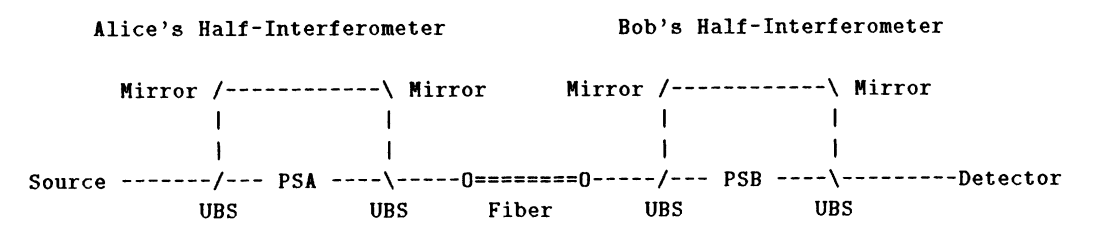
\includegraphics[width=\linewidth]{images/B92 scheme from article.png}
    \caption{Интерферометрическое квантовое распределение ключей с использованием двух неортогональных низкоинтенсивных когерентных состояний. Источник слева поставляет когерентный импульс (волнообразная форма -W-) с интенсивностью ожидаемых фотонов M) 1 в полуинтерферометр Алисы, где несимметричные разделители пучков (UBS), зеркала и фазовый модулятор (PSA 0 или 180 градусов) производят слабый сигнальный импульс (волнообразная форма -w- или, сдвинутый по фазе, -m-), за которым следует яркий опорный импульс -\%-. Отправленные к Бобу через одномодовое оптическое волокно, импульсы входят в полуинтерферометр Боба, где в зависимости от того, является ли сумма фазовых сдвигов Алисы и Боба (PSA+PSB) равной 0 или 180 градусов, сигнальный импульс проходит через верхнее  или нижнее плечо интерферометра и происходит констурктивная или деструктивно интерференция с ослабленным опорным импульсом перед входом в детектор. Перед этим интерференционным импульсом прибывает очень тусклый импульс (не показан), ослабленный как Алисой, так и Бобом, но ни разу не задержанный. После интерференционного импульса прибывает яркий дважды задержанный опорный импульс (волнообразная форма -W-), который Боб контролирует, чтобы убедиться, что опорные импульсы не подавляются. Также не показаны два неиспользуемых пучка, выходящих из правого делителя пучка  каждого полуинтерферометра вниз.}
    \label{fig:B92 sch lit}
\end{figure}
На рисунке \ref{fig:B92 sch lit} показана практическая интерферометрическая реализация, в которой два неортогональных состояния $(\ket{\mu_1})$ и $(\ket{\mu_2})$ представлены слабыми когерентными световыми импульсами, различающимися по фазе относительно сопровождающего яркого эталонного импульса (яркие когерентные состояния, обычно почти ортогональные, становятся значительно неортогональными, когда их ослабляют до ожидаемой интенсивности одного фотона, потому что все такие слабые состояния включают значительную компоненту состояния нулевого количества фотонов). Начиная слева на рисунке, Алиса использует ряд несимметричных делителей пучка и зеркал, чтобы разделить начальный когерентный импульс на два импульса, разделенных во времени: слабый сигнальный импульс интенсивностью p $\neq$ 1 ожидаемый фотон, за которым следует яркий эталонный импульс с M $\neq$ 1 ожидаемым фотоном. Сигнальный импульс сдвигается фазово (PSA) на 0 или 180 градусов для кодирования битов 0 и 1, затем запускается в одномодовое оптическое волокно. Более яркий эталонный импульс не сдвигается по фазе, но задерживается на фиксированное время ht, затем также запускается в то же волокно. На приемном конце аппарата Боб использует полуинтерферометр, аналогичный Алисе, чтобы снова разделить входной пучок, в том же соотношении, что и ранее, на слабую и яркую части. Как и ранее, слабая часть сдвигается по фазе (PSB) на 0 или 180 градусов, случайным образом и независимо от фазовых сдвигов Алисы, в то время как яркая часть задерживается на ht. Наконец, две части приводятся в интерференцию при входе в детектор.
Волна, входящая в детектор, состоит из трех импульсов, разделенных временем $\Delta$t. Первый импульс, очень слабый импульс, который был ослаблен как Бобом, так и Алисой, но не задержан ни одним из них, далее не рассматривается.
Второй импульс, содержащий важную ключевую информацию, представляет собой слабый импульс, состоящий из суперпозиции луча, задержанного Алисой и ослабленного Бобом, и луча, задержанного Бобом и ослабленного Алисой. Если фазовые сдвиги Алисы и Боба равны, произойдет конструктивная интерференция, и суперпозиционный импульс сгенерирует счет с вероятностью, равной $4T_q$ ожидаемых фотонов, где T - коэффициент передачи волокна, а q - квантовая эффективность детектора. Если фазовые сдвиги Алисы и Боба отличаются, интенсивность суперпозиционного импульса будет намного ниже, идеально - ноль в пределе идеального выравнивания интерферометра (время когерентности источника света здесь не имеет значения, поскольку два интерферирующих импульса точно пропорциональны, будучи ослабленными версиями одного и того же исходного импульса).
Наконец, с задержкой $\delta$ t после суперпозиционного импульса к детектору Боба приходит яркий импульс, который был задержан как Алисой, так и Бобом, но не был ослаблен ни одним из них. Боб подтверждает его прибытие, с приблизительной ожидаемой интенсивностью MT, что он может сделать надежно, если M$T_q$) 1. Этот третий импульс не содержит фазовой информации, но служит для подтверждения того, что опорный импульс действительно прибыл. Таким образом, он защищает от атаки, при которой подслушиватель ("Ева") измеряет каждую пару сигнально-опорных импульсов прибором, аналогичным прибору Боба, повторно передает корректно сфабрикованную пару импульсов, когда ей это удается, и подавляет как сигнальный, так и опорный импульсы, когда это не удается, таким образом, подслушивая канал без создания ошибок в последующих результатах измерений Боба. Ива не может подавить опорный импульс без немедленного обнаружения. Но если она подавит только сигнальный импульс, неподавленный опорный импульс все равно вызовет счет в детекторе Боба с вероятностью pTq, и половина этих счетов приведет к ошибкам в ключе Боба.
Кодирование каждого бита в разнице фаз между слабым сигнальным импульсом и сопровождающим его ярким опорным импульсом предоставляет практический способ реализации операторов, аналогичных Po и P~, которые дают гарантированный нулевой результат только для двух законных сигналов ($\mu_i$) и ($\mu_o$), соответственно, но не для фальшивых сигналов (например, вакуумного состояния), которые подслушиватель может подменить. Разделение сигнальных и опорных импульсов по времени также позволяет им передаваться через один и тот же оптический волоконный кабель, что автоматически компенсирует фазовые дрейфы окружающей среды в кабеле, которые в противном случае сделали бы такой большой интерферометр невыполнимым.

Поскольку любая пара когерентных или не когерентных оптических сигналов значительно становится некоординированной при низкой интенсивности, кажется, что почти любой источник двух видов слабых световых вспышек, например, очень ослабленный красный по сравнению с зеленым светофором, можно использовать для распределения ключей без сложностей интерферометрии. Алиса случайным образом отправляет красные и зеленые вспышки с интенсивностью 1 фотон, а Боб публично сообщает, какие вспышки он видел, но не их цвета, которые составляют секретный ключ. Из-за низкой интенсивности Боб может быть уверен, что пассивный злоумышленник, стоящий рядом с ним и наблюдающий за тем же источником сигнала, не увидит того же подмножества импульсов, и, следовательно, будет иметь не всю информацию о ключе, который будет согласован  Алисой. 
Однако более вторженческая Ева, стоящая между Алисой и Бобом, может полностью нарушить схему, перехватывая все вспышки Алисы и пересылая вспышку Бобу только тогда, когда сама видит вспышку Алисы, просто останавливая остальные. Чтобы компенсировать их уменьшенное количество, поддельные вспышки Евы должны быть пропорционально ярче, так чтобы вероятность Боба видеть оставалась той же самой (осторожная Ева должна была бы создавать вспышки с не-Пуассоновской статистикой числа фотонов, чтобы имитировать распределение Пуассона с меньшим средним значением). В терминах формализма операторов проекции, обсуждаемого ранее, схема с красным и зеленым не работает, потому что два сигнала, которые Алиса отправляет здесь, не являются чистыми состояниями, а являются статистическими смесями, в которых фаза электрического поля случайна. Поэтому любой оператор Po, который уничтожает все красные вспышки Алисы, также уничтожит вакуумное состояние, поскольку его можно рассматривать как суперпозицию двух красных вспышек с противоположной фазой. Таким образом, Ева может безопасно заменять вакуумное состояние на любую вспышку, которую она не обнаруживает. В отличие от этого, в интерферометрической схеме на рисунке \ref{fig:B92 sch lit} нет поддельного сигнала, который могла бы подменить подслушивающая сторона, чтобы скрыть свое неудачное обнаружение первоначального сигнала, и схема остается надежной. Эти соображения можно обобщить, чтобы заключить, что распределение ключей возможно не только с использованием любых двух некоординированных чистых состояний ($\mu_n$) и (u ), но и любых двух некоординированных смешанных состояний po и p которые охватывают не пересекающиеся подпространства гильбертова пространства, позволяя Бобу найти два оператора Po и P, таких что Po уничтожает p и P уничтожает $P_0$, но никакое состояние не уничтожается обоими операторами. Требование охвата не пересекающихся подпространств отсутствует в схемах распределения ключей, использующих более двух смешанных состояний, позволяя таким схемам (например, схеме, которая использует четыре некоординированных не когерентных состояния) быть реализованными с помощью простого квадратичного обнаружения оптических сигналов, а не интерферометрического гомодинного обнаружения, как в рисунке \ref{fig:B92 sch lit}

\subsection{Протокол квантовой коммуникации с использованием недоверенного приемного узла} \label{sec:ch1/sect2/MDI QKD}
Существующие протоколы квантовой коммуникации строятся на топологии "точка-точка", в которых участвует всего 2 пользователя: приемник и передатчик. Однако у такого подхода есть уязвимости, связанные  с возможностью злоумышленника контролировать детектор одиночных фотонов, используемого в блоке приемника. Или же использовать другие каналы утечки информации из-за несовершенства детектора одиночных фотонов: различный временной отклик, наличие обратной вспышки при регистрации фотона. Как решение всех известных уязвимостей детекторов одиночных фотонов был разработан протокол КРК с недоверенным приемным узлом (НПУ-КРК) или же Measurement-Device-Independent Quantum Key Distribution (MDI-QKD). 
\newline В данной работе представлена идея квантовой криптографии с измерениями, независимыми от устройства (MDI-QKD) \cite{lo2012,liu2013}, как простое решение для устранения всех (существующих и еще не обнаруженных) каналов утечки информации, связанных с детектором \cite{zhao2008}, пожалуй, самой критической части реализации, и показываем, что у нее как отличные показатели безопасности, так и производительности. Таким образом, она предлагает огромное преимущество в безопасности по сравнению со стандартными доказательствами безопасности, такими как доказательства Инамори-Люткенхауса-Майерса (ILM) \cite{inamori2007} и Готтесмана-Ло-Люткенхауса-Прескилла (GLLP). \cite{gottesman2004} Более того, данный подход позволяет удвоить дальность передачи, которую могут покрыть те схемы квантовой криптографии, которые используют обычные полупроводниковые лазеры, а ее скорость генерации ключей сравнима со стандартными доказательствами безопасности с использованием запутанных пар. В отличие от квантовой криптографии с прямыми измерениями (DI-QKD), в ее простейшей формулировке MDI-QKD требует дополнительного предположения о том, что у Алисы и Боба почти идеальная подготовка состояний. Однако это не препятствие, потому что источники сигнала Алисы и Боба могут быть ослабленными лазерными импульсами, подготовленными ими самими. Их состояния могут быть экспериментально проверены в полностью защищенной лабораторной среде за пределами вмешательства Евы через случайную выборку. Более того, как будет обсуждаться позже, недостатки в процессе подготовки Алисы и Боба на самом деле могут быть легко устранены в более точной формулировке протокола.
\newline Простой пример нашего метода следующий. Как Алиса, так и Боб подготавливают слабые когерентные импульсы (СКИ) с фазовым кодированием в четырех возможных поляризационных состояниях BB84 (т. е. вертикальном, горизонтальном, поляризованном под углом 45 и 135 градусов) \cite{bennett1984} и отправляют их ненадежному ретранслятору Чарли (или Еве), находящемуся посередине, который выполняет измерение состояния Белла, проецирующее входные сигналы в состояние Белла. Такое измерение может быть реализовано, например, с использованием только линейных оптических элементов с установкой, показанной на рисунке \ref{fig:MDI scheme lit} (На самом деле, такая установка определяет только два из четырех состояний Белла. Но это не проблема, поскольку любое состояние Белла позволяет доказать безопасность.) Кроме того, Алиса и Боб применяют методы фальшивых состояний, чтобы оценить усиление (т. е. вероятность успешного результата ретранслятора) и квантовую погрешность бита (QBER) для различных чисел входных фотонов. После завершения квантовой коммуникационной фазы Чарли использует открытый канал для объявления событий, где он получил успешный результат в ретрансляторе, а также свой результат измерения. Алиса и Боб сохраняют данные, соответствующие этим случаям, и отбрасывают остальные. Кроме того, как и в BB84, они на этапе постобработки выбирают события, где они используют тот же базис в своей передаче с помощью аутентифицированного открытого канала. Наконец, чтобы гарантировать, что их битовые строки правильно коррелируются, Алиса или Боб должны применить инверсию бита к своим данным, за исключением случаев, когда они оба выбирают диагональную базу и Чарльз получает успешный результат измерения, соответствующий тройному состояний. Давайте теперь подробно оценим производительность протокола выше. Для простоты рассматривается улучшенный анализ данных, при котором Алиса и Боб оценивают данные, отправленные в двух разных базисах \cite{lo2005}. В частности, используется линейный базис в качестве базиса генерации ключей, в то время как диагональный базис используется только для тестирования.
\begin{figure}
    \centering
    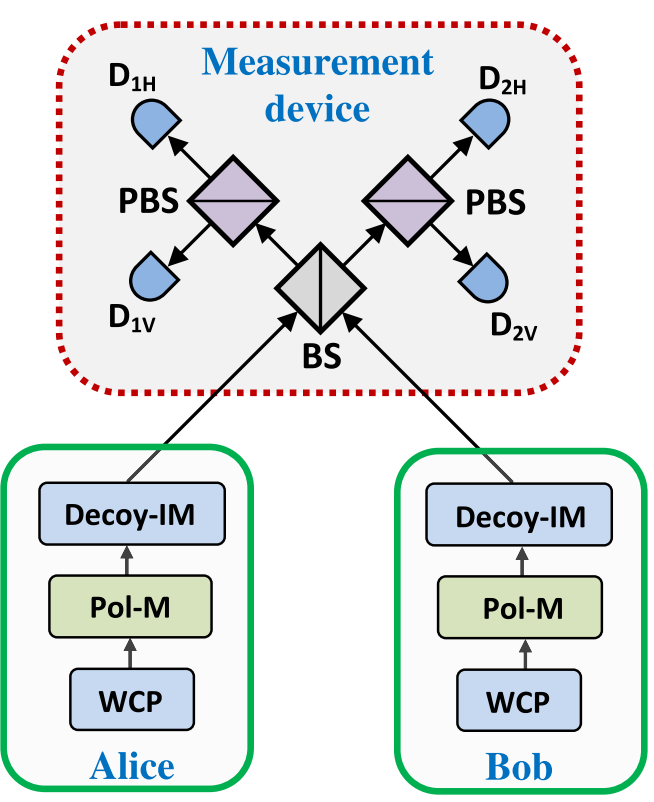
\includegraphics[width=0.7\linewidth]{images/MDi scheme.png}
    \caption{Базовая схема протокола MDI-QKD.
Алиса и Боб подготавливают фазово случайные слабые когерентные импульсы (СКИ) в разных поляризационных состояниях BB84, которые выбираются независимо и случайным образом для каждого сигнала с помощью модулятора поляризации (Pol-M). Состояния - ловушки генерируются с использованием модулятора интенсивности (Decoy-IM). Внутри измерительного устройства сигналы от Алисы и Боба интерферируют на светоделителе  (BS) с коэффициентом деления 50:50, на каждом конце которого находится поляризационный светоделитель (PBS), направляющий входящие фотоны в горизонтальные (H) или вертикальные (V) поляризационные состояния. Четыре фотодетектора используются для обнаружения фотонов, и результаты обнаружения объявляются публично. Успешное измерение состояния Белла соответствует наблюдению активации ровно двух детекторов (связанных с ортогональными поляризациями). Клик в $D_{1H}$ и $D_{2V}$ или в $D_{1V}$ и$D_{2H}$ указывает на проекцию на состояние Белла $\ket{\psi^{-}} = \frac{1}{\sqrt{2}}(\ket{HV} - \ket{VH})$, в то время как клик в $D_{1H}$ и $D_{1V}$ или в $D_{2H}$ и $D_{2V}$ показывает проекцию на состояние Белла $\ket{\psi^{+}} = \frac{1}{\sqrt{2}}(\ket{HV} + \ket{VH})$. Установки Алисы и Боба надежно защищены от прослушивателя, в то время как измерительное устройство может быть ненадежным.
}
\end{figure} \label{fig:MDI scheme lit}
\newline Для обзоначений введем $Q_{rect}^{n,m} , Q_{diag}^{n,m} , e_{rect}^{n,m} , e_{diag}^{n,m}$ - обозначают, соответственно, усиление и QBER сигнальных состояний, отправленных Алисой и Бобом, где n и m обозначают количество фотонов, отправленных законными пользователями, а rect или diag представляет их выбор базиса.
\newline (A) Прямоугольный базис. Ошибка соответствует успешному выводу ретранслятора, когда и Алиса, и Боб подготавливают одно и то же поляризационное состояние (т. е. их результаты должны быть антикоррелированы до применения инверсии бита). Предполагая на данный момент идеальные оптические элементы и детекторы, и отсутствие смещения, имеем, что каждый раз, когда Алиса и Боб отправляют, соответственно, n и m фотонов, подготовленных в одном и том же поляризационном состоянии, ретранслятор никогда не выдаст успешный результат. Таким образом, получаем, что $e_{rect}^{n,m}$
 равно нулю для всех n, m. Это означает, что для отфильтрованного ключа не требуется коррекция ошибок. Это замечательно, потому что это подразумевает, что использование источников СКИ (вместо однофотонных источников) не существенно снижает скорость генерации ключей протокола квантовой криптографии (в части коррекции ошибок).
\newline (B) Диагональный базис. Чтобы определить количество необходимой амплификации конфиденциальности, рассматривается диагональный базис. Ошибка соответствует проекции на синглетное состояние в случае, когда Алиса и Боб подготавливают одно и то же поляризационное состояние, или на тройное состояние, когда они подготавливают ортогональные поляризации. Предполагая опять же идеальный сценарий, обсуждаемый в предыдущем абзаце, находим, что $e_{diag}^{1,1}$ = 0. (Это происходит потому, что когда два идентичных однофотонных входят в 50:50 светоделитель, эффект Хонга-Оу-Манделя \cite{hong1987} гарантирует, что оба фотона всегда выйдут из светоделителя вместе в том же самом выходном режиме. Кроме того, если два фотона подготовлены в ортогональных поляризациях и они выходят из 50:50 светоделителя в том же самом выходном плече, оба фотона всегда достигнут одного и того же детектора внутри ретранслятора.) Тот факт, что $e_{diag}^{1,1}$ равно нулю, вновь поразителен, так как это означает, что использование источников СЦИ существенно не снижает скорость генерации ключей (также в части усиления секретности).
\newline (C) Скорость генерации ключей. В идеальном сценарии, описанном выше, скорость генерации ключей будет просто определяться как $R = Q_{rect}^{1,1}$ в асимптотическом пределе бесконечно длинного ключа. С другой стороны, если учитываются недостатки, такие как смещение базиса и темные отсчеты, скорость генерации ключей в реалистичной настройке будет определяться как
\begin{align}
    R = Q_{rect}^{1,1}[1-H(e_{diag}^{1,1})] - Q_{rect}f(E_{rect})H(E_{rect})
\end{align} \label{eq:MDI key rate},
где $Q_{rect}$ и $E_{rect}$ обозначают, соответственно, усиление и QBER в прямоугольном базисе ( то есть $  Q_{\text{rect}} = \sum_{n,m} Q_{\text{rect}}^{n,m}  $ и $E_{\text{rect}} =\sum_{n,m} \frac{Q_{rect}^{n,m}e_{rect}^{n,m}}{Q_{rect}}$, $\text{f}(E_{rect}) > 1$ функция неэффективности для процесса коррекции ошибок, а $H\text{(x)} = - x\log_2(x) - (1 - x)\log_2(1-x) $  функция бинарной энтропии Шеннона. Есть несколько нерешенных вопросов, которые нужно прояснить. Во-первых, предполагается, что метод фальшивых состояний можно использовать для оценки усиления $Q_{rect}^{1,1}$ и QBER $e_{rect}^{1,1}$. 
\begin{figure}
    \centering
    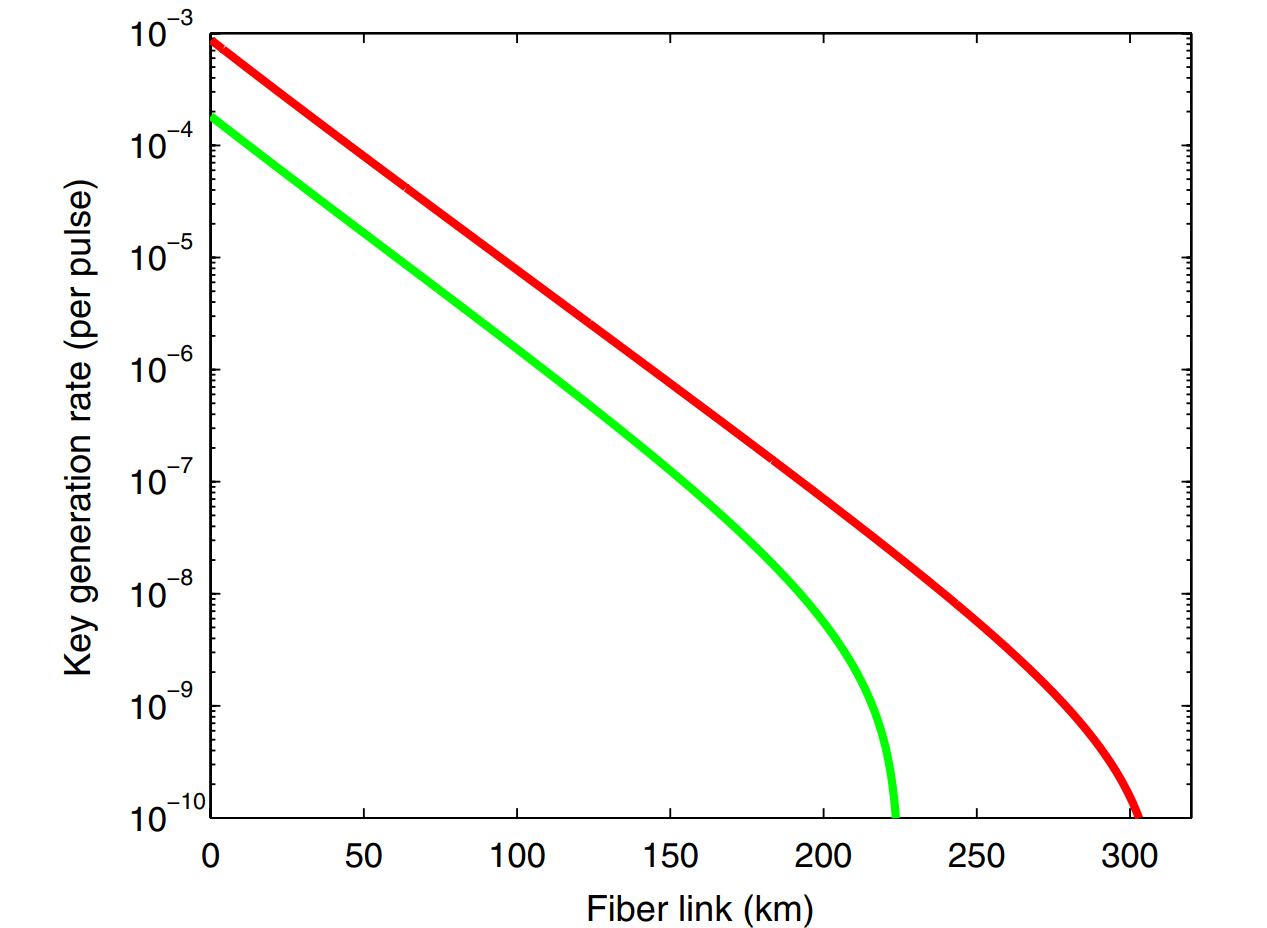
\includegraphics[width=0.8\linewidth]{images/mdi speed.png}
    \caption{Нижняя граница секретной скорости ключа R, заданная уравнением \ref{eq:MDI key rate}, в логарифмической шкале для установки MDI-QKD с использованием слабых когерентных импульсов, показанной на рисунке \ref{fig:MDI scheme lit} (зеленая кривая). В целях моделирования рассматриваются следующие экспериментальные параметры: коэффициент потерь канала составляет 0,2 дБ/км, внутренняя ошибка из-за смещения и нестабильности оптической системы составляет 1,5\%, эффективность обнаружения реле (т. е. пропускная способность его оптических компонентов вместе с эффективностью его детекторов) составляет 14,5\%, а фоновая частота счета составляет 6,02 × $10^(-6)$. (Для простоты рассматривается упрощенную модель смещения, помещая унитарное вращение в одну из входных ветвей светоделителя с делением пополам 50:50 и также унитарное вращение в одну из его выходных ветвей. Общее значение смещения составляет 1,5\%. То есть, мы предполагаем смещение в 0,75\% в каждом вращении.) В сравнении красная кривая представляет нижнюю границу R для протокола квантовой криптографии на основе запутанных пар с источником на основе параметрического преобразования с понижением частоты (PDC), расположенным посередине между Алисой и Бобом \cite{ma2007}. На красной кривой предполагается, что используется оптимальная яркость источника PDC. Однако на практике яркость источника PDC ограничена технологией. Поэтому скорость ключа протокола квантовой криптографии на основе запутанных пар будет значительно ниже, чем показано на красной кривой. Это делает наше новое предложение еще более привлекательным по сравнению с существующими данными на рисунке}
\end{figure} \label{fig:key rate MDI lit}
Во-вторых, нам нужно оценить секретную скорость ключа, заданную уравнением \ref{eq:MDI key rate}, для реалистичного устройства 
Во-вторых, нам нужно оценить секретную скорость ключа, заданную уравнением \ref{eq:MDI key rate}, для реалистичной настройки. Давайте уточним эти моменты здесь. Действительно, можно показать, что метод оценки соответствующих параметров в формуле для скорости ключа эквивалентен используемому в стандартных системах квантовой криптографии с фальшивыми состояниями. Для целей моделирования рассматриваются неэффективные и шумные пороговые детекторы и используем экспериментальные параметры из \cite{takeoka2014} за исключением того, что \cite{takeoka2014} рассматривает канал свободного пространства, тогда как здесь рассматривается канал на основе оптоволокна с потерей 0,2 дБ/км. Более того, для простоты предполагается, что все детекторы идентичны (т.е. у них одинаковая частота темных отсчетов и эффективность обнаружения), и их темные отсчеты, приблизительно, независимы от входящих сигналов. Кроме того, используется протокол коррекции ошибок с функцией неэффективности $\text{f}(E_{rect})$ = 1,16 \cite{pirandola2017}. Полученная нижняя граница секретной скорости ключа проиллюстрирована на рисунке \ref{fig:TF key rate lit}. Наши расчеты и результаты моделирования показывают, что скорость генерации ключей существенно сравнима с доказательством безопасности \cite{ma2007} для протоколов квантовой криптографии на основе запутанных пар. Наша схема может выдерживать высокие оптические потери более 40 дБ или 200 км ВОЛС, если ретранслятор размещается посередине между Алисой и Бобом. Другими словами, можно практически удвоить дистанцию передачи по сравнению с установкой, где аппарат измерения состояния Белла находится у Алисы, или установкой с использованием стандартного протокола BB84 с фальшивыми состояниями.
Чтобы экспериментально реализовать предложенный протокол MDI-QKD, несколько практических вопросов требуют решения. Среди них, возможно, самый важный - это то, как генерировать неразличимые фотоны из двух независимых лазерных источников и наблюдать стабильное интерференционное явление Хонга-Оу-Манделя \cite{hong1987}. Обратите внимание, что физика, лежащая в основе этого протокола, основана на явлении группировки фотонов в одну группу двух неразличимых фотонов на 50:50 светоделителе. Здесь проводится простой эксперимент принципиального доказательства, чтобы показать, что высокая видимость интерференции Хонга-Оу-Манделя между двумя независимыми лазерами, которые возможно приобрести, вполне осуществима. Результаты показаны на рисунке \ref{fig:TF key rate lit}. Согласованность между экспериментальными и теоретическими результатами подтверждает, что высокая видимость интерференционного провала Хонга-Оу-Манделя может быть достигнута даже с двумя независимыми лазерами.
Идею MDI-QKD можно обобщить намного дальше. Во-первых, она также применима в случае, когда Алиса и Боб используют запутанные пары фотонов в качестве источников. Во-вторых, она работает даже в том случае, когда процессы подготовки Алисы и Боба неидеальны. Действительно, зависимость от базиса, возникающая из недостатка в процессах подготовки Алисы и Боба, может быть легко устранена с помощью идеи квантовой монетки \cite{gottesman2004,koashi2005}, чтобы количественно оценить количество зависимого от базиса недостатка \cite{tamaki2012}. В-третьих, заметим, что в практических приложениях потребуется только конечное количество фальшивых состояний. Это аналогично стандартным протоколам квантовой криптографии с конечными фальшивыми состояниями \cite{ma2005}, которые широко используются в экспериментах \cite{rosenberg2009}. В-четвертых, MDI-QKD работает даже без уточненного анализа данных. В-пятых, она также работает для других протоколов квантовой криптографии, включая протокол из шести состояний \cite{fuchs1997}. Эти вопросы, вместе с учетом эффектов конечного размера, возникающих потому, что Алиса и Боб отправляют только конечное количество сигналов в каждом запуске протокола квантовой криптографии\cite{tamaki2012}.

В заключение, предлагается идея квантовой криптографии с измерительно-устройствонезависимым подходом (MDI-QKD). По сравнению со стандартными доказательствами безопасности, у него есть ключевое преимущество в удалении всех каналов боковых сигналов детектора, и он может удвоить дистанцию передачи, охватываемую с помощью обычных протоколов квантовой криптографии с использованием слабых когерентных импульсов. Более того, у него довольно высокая скорость генерации ключей, которая сравнима с таковой в стандартных доказательствах безопасности. Действительно, его скорость генерации ключей на порядки выше, чем предыдущий подход полностью измерительно-устройствонезависимой квантовой криптографии. Нашу идею можно реализовать с помощью стандартных пороговых детекторов с низкой эффективностью обнаружения и каналов с высокими потерями. Учитывая его отличную безопасность, производительность и простую реализацию, считается что MDI-QKD является большим шагом вперед в сокращении разрыва между теорией и практикой квантовой криптографии, и ожидаем, что он будет широко применяться в практических системах квантовой криптографии в будущем.
\subsection {Протокол квантовой коммуникации с использованием полей близнецов}\label{sec:ch1/sect2/TF QKD lit}
Значительный теоретический прогресс в достижении практического безопасного QKD на больших расстояниях был достигнут с предложением QKD с двойным полем (TFQKD)\cite{scarani2009}, которое улучшает масштабирование ключевой скорости в соответствии с квадратным корнем из пропускания канала. Он показывает, что источник когерентного состояния на самом деле может быть преимуществом по сравнению с однофотонным источником, поскольку постселекция фазовой когерентности двойных полей Алисы и Боба может потенциально привести к безопасному QKD с кодирующим состоянием одного фотона и вакуума, а также их линейных суперпозиций. Этот метод способен достичь скорости передачи ключей, зависящей от квадратного корня из коэффициента пропускания канала, и, таким образом, преодолеть известное ограничение по расстоянию для существующих протоколов практического QKD. Теоретически безопасная ключевая скорость может быть даже выше, чем возможности секретных ключей без ретрансляторов, известные как границы Такеока-Гуха-Вильде \cite{takeoka2014} и Пирандола-Лауренца-Оттавиани-Бьянки (PLOB) \cite{pirandola2017}. Однако для того, чтобы сделать это реальностью, еще предстоит проделать значительную работу. Во-первых, существует теоретическая проблема объединения постселекции фазовой информации с традиционным методом ложных состояний. Во-вторых, это технически сложная задача точной интерференции одиночных фотонов на большом расстоянии. Для достижения этой цели был предложен протокол "посылать или не посылать" (SNS) \cite{wang2018}. Он предполагает малые вероятности отправки для Алисы и Боба, а затем использует решения об отправке и отказе от отправки для кодирования битовых значений в базисе Z с эффективными событиями-вестниками, объявляемыми Чарли. Таким образом, как было показано в \cite{wang2018}, в протоколе можно продолжать использовать модель с метками и обычный метод ложных состояний. Кроме того, поскольку протокол кодирует битовые значения, используя почти безошибочный базис Z, он может терпеть высокую частоту ошибок в базисе X. 
\begin{figure}
    \centering
    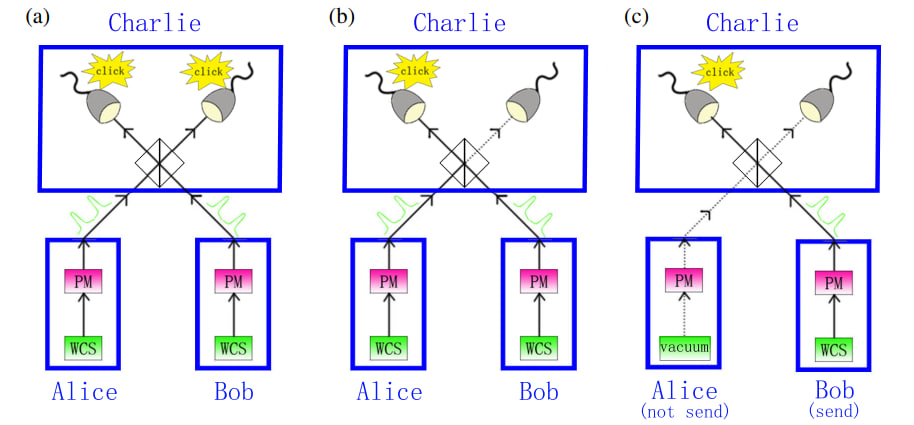
\includegraphics[width=\linewidth]{images/TF schemes lit.jpg}
    \caption{Схемы трех различных протоколов. (a) MDIQKD с состояниями-ловушками, где пары импульсов с когерентным состоянием в кодировке BB84 рассылаются, а эффективные события предвещаются двукратным срабатыванием. Скорость передачи ключей линейно зависит от пропускания канала. (b) Оригинальное состояние приманки TFQKD \cite{lucamarini2018}, в котором сдвоенные поля когерентных состояний со случайными фазовыми сдвигами посылаются по базам X и Y, а эффективные события возвещаются одиночным щелчком. Скорость передачи ключей зависит от квадратного корня из пропускания канала. Для обоих базисов необходимы однофотонные помехи от удаленных независимых источников. Возможны ошибки рассогласования в обеих базах, и информация о фазовом сдвиге после объявления делает метод "приманка-состояние" недействительным. (c) SNSTFQKD (Sending - not sending TFQKD) с состояниями ловушками \cite{ma2005}. В базисе Z каждая сторона независимо принимает решение об отправке с небольшой вероятностью. События, когда одна сторона решает отправить, другая сторона решает не отправлять, и один и только один детектор щелкает (как показано на рисунке), являются целевыми событиями для генерации защищенных ключей. Он отказоустойчив к большой ошибке смещения в базисе X, так как ошибка смещения в базисе Z отсутствует. Традиционный метод "приманка-состояние" работает, поскольку информация о фазовом сдвиге в базисе Z никогда не объявляется. Объявление одного щелчка делает эффективными события в базисе Z, а ключевая скорость находится в масштабе квадратного корня из пропускания канала. WCS: слабый когерентный источник}
    \label{fig:TF protocols scheme}
\end{figure}
В этой работе рассматривается экспериментальная демонстрация КРК с полями-близнецами через протокол SNS (SNSTFQKD) по катушкам оптического волокна.
Протокол.- Рассмотрим схему протокола SNSTFQKD \cite{ma2007}, показанную на рисунке \ref{fig:TF protocols scheme}. Здесь реализуется протокол с помощью практического метода четырех интенсивностей \cite{gobby2004}, где каждая сторона использует четыре различные интенсивности, а именно 0, $\mu_1$, $\mu_2$ и $\mu_z$. Алиса и Боб случайным образом выбирают базис X или Z с вероятностями pX и 1 - pX, соответственно. В базисе X Алиса и Боб готовят и посылают импульсы-обманки. Фазовые сдвиги $\theta_A$ и $\theta_B$ частным образом накладываются на их импульсы. Событие в базисе Z считается эффективным, если Чарли объявляет, что щелкнул только один детектор. Для того чтобы событие X-базиса было эффективным, нам необходимо дополнительное условие фазового среза, чтобы уменьшить наблюдаемую частоту ошибок в базисе. Без разумного условия фазового среза наблюдаемый коэффициент ошибок в базисе X может быть слишком большим, чем фактический коэффициент ошибок в базисе Z. Обратите внимание, что Чарли не обязан быть честным, и все, что он объявляет, не подрывает безопасность. Но если Чарли хочет получить высокую скорость генерации секретного ключа, ему придется постараться сделать правдивое объявление обо всем. Ошибка в базисе X определяется как объявление Чарли о щелчке правого (левого) детектора, связанном с эффективным событием в базисе X, когда разница фаз между парой импульсов от Алисы и Боба, вероятно, вызвала бы щелчок слева (справа) на измерительной установке Чарли. Эффективное событие в базисе Z, которое Алиса (Боб) решила отправить, а Боб (Алиса) решил не отправлять, соответствует значению бита 1 (0). Значения $\epsilon_1^{ph}$ и $s_1$, выход однофотонных эффективных событий в базисе Z, могут быть рассчитаны обычным методом ложных состояний.
\begin{figure}
    \centering
    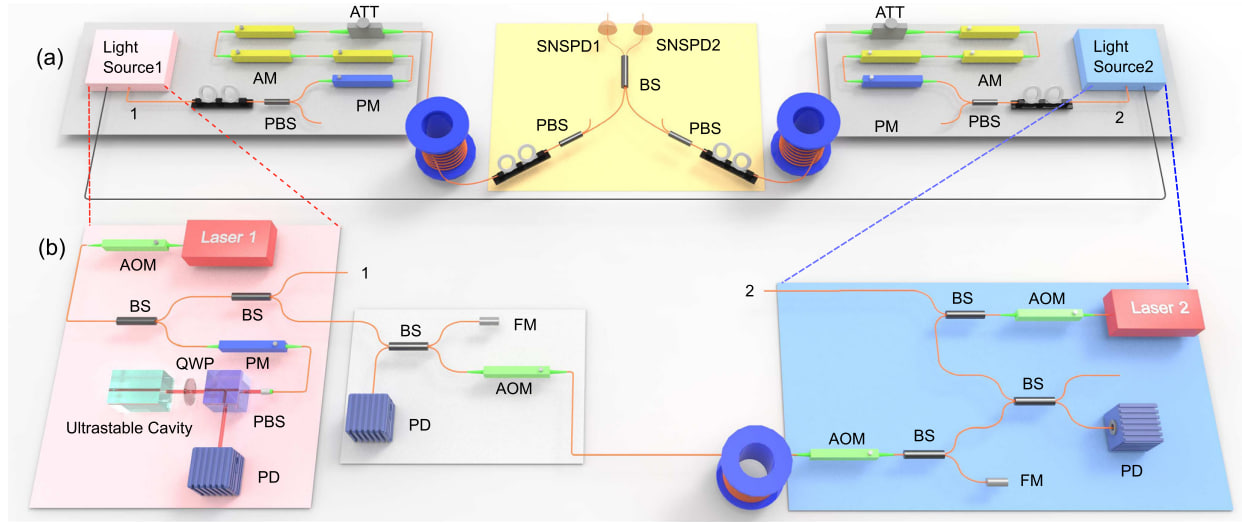
\includegraphics[width=\linewidth]{images/TF experiment scheme.jpg}
    \caption{(a) Схема нашей экспериментальной установки. В качестве источников Алиса и Боб используют непрерывный лазер с частотной синхронизацией.  Эти лазеры затем модулируются фазовым модулятором (ФМ) и тремя амплитудными модуляторами (АМ) для рандомизации фазы, кодирования и модуляции интенсивности обманки. Затем импульсы ослабляются аттенюатором (ATT) и отправляются по оптоволоконным катушкам к Чарли. На измерительной станции Чарли На измерительной станции Чарли импульсы от Алисы и Боба проходят через поляризационные контроллеры (PC) и поляризационные разветвители луча (PBS), затем интерферируют на разветвителе луча (BS). Наконец, свет измеряется сверхпроводящими нанопроволочными однофотонными детекторами (SNSPD). (b) Система частотной синхронизации для лазеров Алисы и Боба. Длина волокна между Алисой и Бобом установлена равной общей длина сигнального волокна. AOM: акустооптический модулятор, FM: зеркало Фарадея, PD: фотодиод. QWP: четвертьволновая пластина.}
    \label{fig:TF experiment scheme}
\end{figure}
Схема эксперимента показана на рисунке \ref{fig:TF experiment scheme}(a). В установках Алисы и Боба в качестве источников света используются независимые лазеры с непрерывной волной (cw). Свет модулируется на 16 различных фаз с помощью фазового модулятора (ФМ) и кодируется с помощью трех амплитудных модуляторов (АМ). В эксперименте устанавливается базовый период 5 мкс, в течение которого в первые 3 мкс посылается 100 сигнальных импульсов с шириной импульса 2 нс и интервалом 30 нс, затем в следующие 1,2 мкс - 4 фазовых опорных импульса для оценки относительной фазы между каналами Алисы и Боба, и в заключительные 0,8 мкс - состояние вакуума в качестве времени восстановления сверхпроводящих нанопроволочных однофотонных детекторов (SNSPDs). Интенсивности сигналов устанавливаются в оптимизированные состояния приманки $\mu_z$, $\nu_1$, $\nu_2$ или 0 . Затем сигналы передаются от Алисы и Боба к Чарли, где они интерферируют. Поскольку для интерференции требуются идентичные входные сигналы, для компенсации поляризационного дрейфа канала необходимы поляризационные контроллеры (PC) и поляризационные разветвители луча (PBS) перед поляризационными поддерживающими разветвителями луча (BS). Результаты интерференции затем обнаруживаются с помощью SNSPD и регистрируются с помощью высокоскоростного устройства регистрации времени. Основной технической проблемой при реализации SNSTFQKD является управление фазовой эволюцией полей-близнецов. Как было указано в, дифференциальное колебание фазы между двумя пользователями может быть записано как
\begin{align}
    \delta_{ba} = \frac{2\pi}{s}(\delta\nu L + \nu\delta L)
\end{align}\label{eq: TF phase fluct lit},
 где $\nu$- оптическая частота света, L - длина волокна, s - скорость света в волокне. Таким образом, необходимо компенсировать два источника, вносящих вклад в разность фаз: первый член в уравнении обозначает разность частот между Алисой и Бобом, а второй - дрейф фазы в волокне. В качестве примера, измеренная скорость дрейфа фазы соответствует гауссову распределению со стандартным отклонением 7,4 рад $мс^{-1}$ для общего расстояния волокна 150 км. Чтобы справиться с разницей фаз, вызванной разницей длин волн, используется метод частотной синхронизации, как показано на рисунке \ref{fig:TF experiment scheme}(b). В лаборатории Алисы в качестве начального лазера используется лазер непрерывной волны с центральной длиной волны 1550,12 нм и шириной линии в несколько килогерц. Начальный лазер фиксируется в ультрастабильном резонаторе длиной 10 см с тонкостью около 250 000 с помощью техники Паунда-Древера-Холла, чтобы подавить его ширину линии с нескольких килогерц до примерно десяти герц. Затем свет разделяется на две части, одна из которых используется в качестве источника Алисы, а другая - для блокировки оптической частоты Боба. Этот блокирующий луч далее разделяется на две части, одна из которых отражается от зеркала Фарадея (FM) в качестве локального эталона, а другая частотно-модулируется акустооптическим модулятором (AOM) и отправляется Бобу. Здесь длина волокна установлена равной расстоянию передачи сигнала, чтобы продемонстрировать практичность системы.

 Вместо того чтобы активно стабилизировать относительную фазу между Алисой и Бобом, разница фаз компенсируется с помощью постобработки. Определив оценочную относительную фазу между волокнами Алисы и Боба как $\Delta\phi_T$, вычисляется квантовый коэффициент битовых ошибок в базисе X для обнаружений, лежащих в диапазоне 
 \begin{align}
    1 - |\cos(\theta_A - \theta_B + \delta\phi_T| < \Lambda)
\end{align}\label{eq: QBER error TF}
 где $\theta_A (\theta_B)$ - случайная фаза, которой Алиса (Боб) модулирует сигнал, а $\Lambda$ - заданный диапазон. Тогда вычислить безопасную ключевую скорость с эффектом конечного размера данных по следующей формуле:
 \begin{align}
    R = (1 - p_x)^2{2p_z(1-p_z)a_1s_1[1 - H(e_1^{ph})] - fS_zH(E_z)} - \frac{1}{N_{total}}log_2\frac{1}{\epsilon^5}
\end{align}\label{eq: TF qkd rate lit}
 где R - конечная ключевая скорость, $a_1 = \mu_{\zeta}e^{-\mu_{\zeta}}$, $s_1$ - выход эффективных однофотонных событий в базисе Z, $\epsilon_1^{ph}$ - коэффициент фазовой ошибки для событий в базисе Z, $S_Z$ и $E_Z$ - наблюдаемый выход и коэффициент битовой ошибки для базиса Z, $N_{total}$ - общее число посланных сигнальных импульсов, а $\epsilon =10^{-10}$, что соответствует общей вероятности отказа $2*10^{-9}$. Скорость передачи ключей была бы еще выше, если бы мы учитывали только статистические флуктуации. Здесь предполагается, что эффективность исправления ошибок составляет f = 1.1. В работе протестирован SNSTFQKD с общим расстоянием между Алисой и Бобом от 0 до 300 км.  Во всех экспериментах с различными длинами волокон общее количество импульсов, посылаемых Алисой и Бобом, установлено на уровне $7.2*10^{11}$. Достоверные детектирования составляют $6.5*10^{9}$, $2.3*10^{9}$2,3 × 109, $7.6*10^{8}$ и $2.5*10^{9}$ для 0, 50, 100 и 150 км в первом эксперименте и $1.7*10^{9}$, $1.9*10^{8}$  и  $2.4*10^{7}$ для 100, 200 и 300 км во втором эксперименте. 
 \begin{figure}
     \centering
     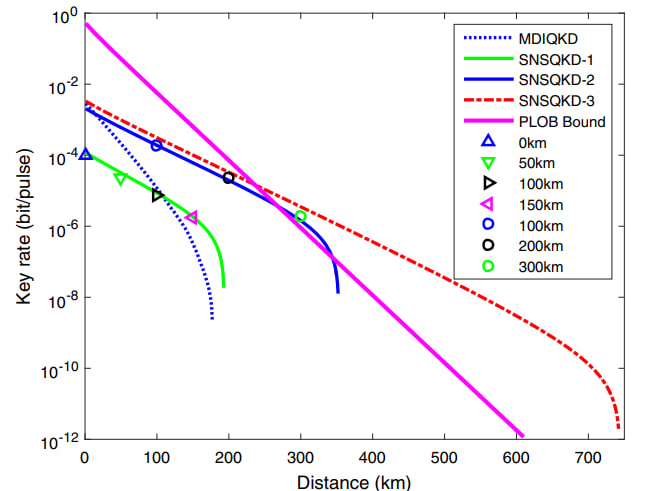
\includegraphics{images/TF key rate lit.jpg}
     \caption{Безопасные ключевые скорости и результаты моделирования SNSTFQKD.
Треугольники показывают экспериментальные результаты для первого экспериментального теста, а сплошная зеленая кривая - результаты моделирования. эксперимента, а сплошная зеленая кривая представляет результаты моделирования
результаты с вероятностью темнового счета около $10^{-6}$ и базовой ошибкой X базиса,  которая составляет около 10 \%. Для сравнения, пунктирная синяя кривая дает результат моделирования протокола MDI-QKD с четырьмя интенсивными приманками протокола MDI-QKD с теми же параметрами, но с
2\% оптических ошибок в базисе X. Кружки показывают экспериментальные экспериментальные результаты для второго теста, а сплошная синяя кривая представляет моделирование с вероятностью темнового счета около
$10^{-7}$ и базовой ошибкой X-базиса около 2 процентов  Общее количество
импульсов, отправленных Алисой и Бобом для всех экспериментальных тестов, составляет
$7.2*10^{11}$ Красная пунктирная кривая далее предполагает, что всего $10^{14}$ импульсов, посланных Алисой и Бобом, с базовой ошибкой X-базиса 2\%. Наконец, сплошная пурпурная линия иллюстрирует границу PLOB.}
     \label{fig:TF key rate lit}
 \end{figure}
 Результаты эксперимента обобщены на рисунке \ref{fig:TF key rate lit}. Сначала экспериментально проверяется SNSTFQKD при вероятности темнового счета $10^{-6}$ (эквивалентно 1000 Гц) и коэффициенте ошибок X-базиса 10 \%. Безопасная ключевая скорость на расстоянии 150 км составляет $1.72*10^{-6}$  на импульс, что уже выше, чем смоделированная безопасная ключевая скорость протокола независимого квантового распределения ключей (MDI-QKD), использующего те же параметры, что и в эксперименте, но предполагающего более низкие $(2\%)$ оптические ошибки в X-базисе. На самом деле, моделирование показывает, что безопасная скорость генерации ключей уже превышает скорость MDI-QKD на расстоянии 108 км.
 Далее снижается вероятность темнового счета примерно до $10^7$ (эквивалентно 100 Гц), модернизировав SNSPD для интеграции полосового фильтра на кристалле внутри, и снизил уровень ошибки X-базиса примерно до 2$\%$, используя линейный усилитель для управления модуляторами. Безопасная скорость передачи ключей на расстоянии 300 км по оптоволокну составляет $1,96 × 10^{-6}$, что выше границы PLOB, равной $8.64 × 10^{-7}$ на импульс. Моделирование показывает, что SNSTFQKD преодолевает эту границу на расстоянии 267 км, а расстояние передачи может превышать 350 км при экспериментальных параметрах. Наконец, моделируется безопасная скорость выработки ключей, предполагая, что всего будет отправлено $10^{14}$ импульсов (с $2.6 × 10^5$достоверными срабатываниями, накопленными на расстоянии 720 км), а вероятность темнового счета однофотонного детектора уменьшена до $10^{-11}$ (эквивалентно 0,1 Гц при длительности импульса 100 пс). Все остальные параметры соответствуют параметрам эксперимента на расстоянии 300 км. Моделирование показало, что максимальное расстояние распространения составляет 742 км, а протокол SNSTFQKD достигает скорости передачи ключей выше границы PLOB, когда расстояние между волокнами превышает 236 км. В заключение разрабатывается технология фазовой синхронизации и фазовой компенсации, экспериментально протестировали протокол SNSTFQKD и продемонстрировали генерацию защищенных ключей на расстоянии до 300 км по оптоволокну, обеспечив скорость передачи ключей, превышающую емкость секретного ключа без ретранслятора. При расчете ключевой скорости были полностью учтены эффекты конечного размера, что гарантирует безопасность в практической ситуации. Отметим, что и расстояние, и ключевая скорость могут быть значительно улучшены за счет использования двусторонней классической связи. Экспериментальные результаты также показывают, что протокол SNSTFQKD устойчив к фазовому рассогласованию, что является важным преимуществом на практике. Метод фазовой синхронизации, использованный в эксперименте, оказался стабильным на расстоянии 1800 км по волокну, а интенсивность опорных фазовых импульсов находилась в пределах нескольких микроватт даже на расстоянии 1000 км. С учетом имеющихся в настоящее время технологий и результатов теоретического моделирования с практическими параметрами ожидается, что в ближайшем будущем будут достигнуты расстояния распространения более 500 км.


\subsection{Протокол квантовой коммуникации на боковых частотах модулированного излучения}\label{sec:ch1/sect2/subsec2}

\section{Когерентное детектирование}\label{sec:ch1/sect3}
Когерентное детектирование - это метод регистрации сигналов, при котором принимаемый сигнал сбивается с мощным опорным сигналом или излучением, называемым локальным осциллятором (ЛО) \cite{ip2008a}. Результат этого смешения регистрируется классическим детектором, например, балансным детектором. К преимуществам данного метода регистрации сигналов  можно отнести следующее: возможность измерения не только амплитуды входного излучения, но и его фазы. В то время как при некогерентном детектировании информация о фазе принимаемого сигнала теряется, то при когерентном детектировании она сохраняется. Эта особенность позволяет переходить к более сложным типам модуляции, что, в свою очередь, повышает эффективность использования полосы сигналов и повышает скорость передачи данных. В то время когда некогерентный метод детектирования не сохраняет информацию и регистрирует только интенсивность приходящего излучения, что ограничивает скорость передачи информации, которая ограничивается полосой пропускания приемника. Другим преимуществом является большая чувствительность, по сравнению с некогерентным квадратичным детектированием. Это достигается за счет того, что ослабленный информационный сигнал, взаимодействуя с мощным ЛО, усиливается и за счет этого достигается большая чувствительность. 
Однако у данного подхода есть и минусы: необходимость дополнительных компенсаций фазовых искажений, связанных с прохождением сигнала в среде распространения и нескоррелированность фазовых шумов источником информационного сигнала и ЛО.  Эти недостатки компенсируются либо дополнительными техническими доработками или цифровой обработкой сигналов (ЦОС), что приводит к расширению использования когерентного детектирования в современных системах передачи данных.
\newline Методы когерентного детектирования можно разделить на несколько категорий по используемым частотам или длин волн информационного сигнала и ЛО. В случае если информационный сигнал передается на той же длине волны, что и локальный осциллятор, то такой метод детектирования называют гомодинным. Подробнее данный способ рассматривается в разделе \ref{sec:ch1/sect3/homodyne lit}.
Если же длины волн информационного сигнала и ЛО разнесены так, что промежуточная их частота больше частоты модулирующего сигнала, то такой способ детектирования называют гетеродинным, подробнее он рассматривается в разделе \ref{sec:ch1/sect3/heterodyne lit}. Существуют и другие методы детектирования, позволяющие компенсировать недостатки гомодинного детектирования - двойное гомодинирование или 90-градусный оптических гибрид. Его суть заключается в том, что и информационный сигнал, и ЛО разделяются пополам и каждая из разделенных частей подается на отдельный делитель, где сбиваются друг с другом, однако в одну из частей ЛО вносят дополнительный фазовый сдвиг, за счет которого можно принимать информацию о любой фазе. Подробнее данный способ регистрации рассматривается в разделе \ref{sec:ch1/sect3/90 hybrid lit}.

\subsection{Гомодинное детектирование}\label{sec:ch1/sect3/homodyne lit}
Гомодинное детектирование - один из методов когерентного детектирования, отличительной чертой которого является равенство длин волн информационного сигнала и локального осциллятора. Нашел широкое применение в оптических системах передачи данных благодаря относительной простоте реализации. Структурная схема такого приемника изображена на рисунке \ref{fig:homodyne det lit}. 
\begin{figure}
    \centering
    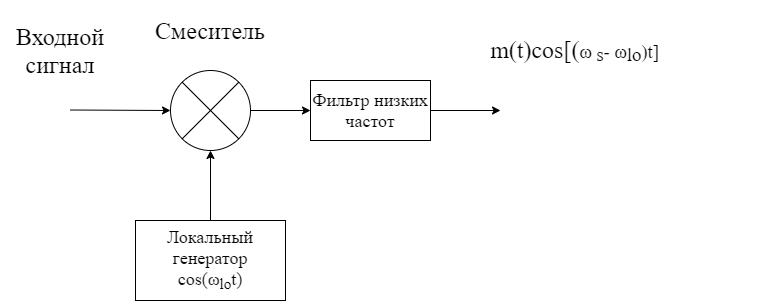
\includegraphics[width=\linewidth]{images/когеретное.png}
    \caption{Структурая схема гомодинного приема}
    \label{fig:homodyne det lit}
\end{figure}

Интенсивность в случае гомодинного детектирования будет описываться следующим выражением
\begin{equation}
    I(t) =|E(t)|^2 =  |E_1|^2 + |E_2|^2 + 2|E_1|\cos[(\omega_1 - \omega_2)t + \phi_1 - \phi_2]
\end{equation}\label{eq: fiedl homodyne}, где $E_1, E_2$ - комплексные амплитуды сигналов информационного и локального осциллятора, $\omega_1, \omega_2$ - частоты информационного сигнала и ЛО, $\phi_1, \phi_2$ - фазы информационного сигнала и ЛО. 
Но так как в случае гомодинного детектирования частоты излучения равны, то результат детектирования приводится к виду 
\begin{equation}
    S(t) = S_0 + S_m\cos(\Delta\phi)
\end{equation}
Таким образом результат интерференции при гомодинном детектировании пропорционален разности фаз между локальным осциллятором и исследуемым сигналом. Однако при $\Delta\phi = 90$ градусов невозможно однозначно различить фазу информационного сигнала и требуется дополнительные технические средства.  
\subsection{Гетеродинное детектирование}\label{sec:ch1/sect3/heterodyne lit}
Другой разновидностью когерентного  детектирования является гетеродинное детектирование. Данный метод нашел свое широкое распространение в радиотехнике c 1917 года под названием супергетеродинный приемник.
\begin{figure}
    \centering
    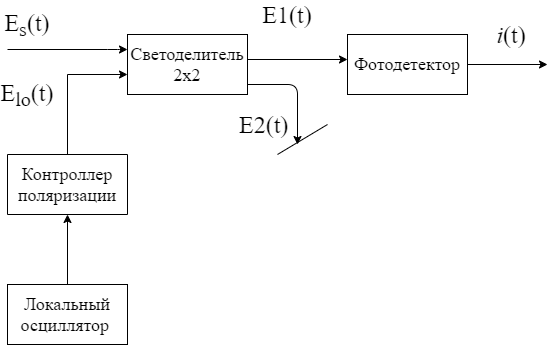
\includegraphics[width=\linewidth]{images/гетеродин для обзора.png}
    \caption{Стурктурная схема гетеродинного оптического приемника}
    \label{fig:heterodyne scheme lit}
\end{figure}
Суть данного метода заключается в следующем. Входной сигнал, несущий информацию подается на один из входов смесителя. На второй же вход смесителя подается сигнал локального осциллятора. При этом частоты входного сигнала и ЛО отличаются. В результате эти два сигнала интерферируют и на выходе смесителя образуется новая частота - промежуточная частота, которая равна разности частот ЛО и входного сигнала. Данный метод описывается следующим образом:
\begin{equation}
    I(t) =|E(t)|^2 =  |E_1|^2 + |E_2|^2 + 2|E_1|\cos[(\omega_1 - \omega_2)t + \phi_1 - \phi_2]
\end{equation}\label{eq: fiedl heterodyne}, где $E_1, E_2$ - комплексные амплитуды сигналов информационного и локального осциллятора, $\omega_1, \omega_2$ - частоты информационного сигнала и ЛО, $\phi_1, \phi_2$ - фазы информационного сигнала и ЛО. 
В результате на выходе фотоприемника формируется сигнал 
\begin{equation}
    S(t) = S_0 + S_m\cos((\omega_1 - \omega_2)t + \Delta\phi)
\end{equation}\label{eq:het result lit}
В выражении \ref{eq:het result lit} присутствует разностная частота $\omega_1 - \omega_2$, которая содержит себе информацию от входного сигнала о его амплитуде и фазе. Благодаря этому, возможно извлекать информацию из сложных типов модуляции, таких как квадртатурно-амплитудная, при этом не прибегая к дополнительным техническим приспособлениям. Данный метод детектирования сигналов является самым гибким для регистрации любых типов модуляции, однако требует точной подстройки частоты и ее стабилизации и фазовой синхронизации между входным сигналом и ЛО для проведения измерений фазы входного сигнала. 
\subsection{90-градусный оптический гибрид }\label{sec:ch1/sect3/90 hybrid lit}
Одним из главных недостатков гомодинного детектирования, описанного в разделе \ref{sec:ch1/sect3/homodyne lit} - является невозможность измерения сигнала с фазой в неортогональном состоянии относительно локального осциллятора. В результате этого при использовании 4 фазовых состояний для кодирования информации, 50 процентов из них будут утеряны из-за невозможности однозначно различить.
Для устранения этого существенного недостатка был разработан метод когерентного детектирования с использованием 90-градусного оптического гибрида или двойного гомодинирования. Данный метод развивает схему гомодинного детектирования из раздела \ref{sec:ch1/sect3/homodyne lit}. Входной сигнал и сигнал ЛО разделяются пополам на двух разных делителях. После этого части входного сигнала смешиваются с частями ЛО. Но в одном из плеч локального осциллятора установлен дополнительный фазовый сдвиг на $\frac{\pi}{2}$. За счет этой модификации возможно измерение фазы принятого сигнала во всех используемых состояниях. Результат измерения попадает на 2 балансный приемника или классических  фотодиода. В результате в том плече, где базисы фаз совпали, сигнал на выходе балансного детектора будет изменяться в зависимости от разности фаз. В другом же плече будет наблюдаться средний уровень сигнала, который невозможно интерпретировать как одно из измеренных фазовых значений. 
Данный метод приема лишен недостатка гомодинного приемника, однако он вносит дополнительные 3 дБ потерь по входному сигналу, что ухудшает его соотношение сигнал - шум, а также удваивает оптическую схему, что негативно сказывается на цене данного метода. Однако такой метод является более предпочтительным, чем одиночный гомодинный приемник. 
\section{Протоколы квантового распределения ключа на непрерывных переменных}\label{sec:ch1/CV-QKD review}
В качестве альтернативы КРК-ДП протоколам, которые в идеале основаны на однофотонном детектировании, КРК-НП \cite{braunstein2005} протоколы кодируют квантовые состояния в непрерывных переменных (НП) лазерного излучения, которые могут быть измерены с помощью гомодинного детектирования с ограниченным уровнем дробового шума. В гомодинном детекторе оптический сигнал подключается к сильному излучению локального осциллятора (ЛО) с ограниченным уровнем шума на сбалансированном делителе луча, и измеряется интенсивность света на выходных портах. В зависимости от разности оптических фаз между сигналом и ЛО, разность фототоков, возникающих в каждом из двух детекторов, будет пропорциональна одной из двух квадратур поля. Таким образом, ЛО несет в себе опорную фазу, которая позволяет переключаться между измерением q- и p-квадратур (или, в более общем случае, выполнять томографию состояния путем измерения функции Вигнера, связанной с состоянием).
Первое предложение об использовании квадратур бозонического поля для реализации КРК появилось в 1999 году, когда Ральф \cite{ralph1999} рассмотрел кодирование ключевых битов с помощью четырех фиксированных квадратурных смещений ярких когерентных или двухмодовых запутанных пучков. Позже Ральф обсудил безопасность двухмодовой схемы на основе запутанности более подробно \cite{ralph2000}, рассматривая не только атаки перехвата-передачи, но и телепортацию НП. Последняя была определена как оптимальная атака на протокол, накладывающая требования высокого сжатия сигнала и низких потерь в канале. Независимо от этого Хиллери \cite{hillery2000} предложил протокол КРК-НП, основанный на квадратурном кодировании одномодового луча, случайным образом сжатого в одном из квадратурных направлений. Безопасность от атак перехвата-передачи и расщепления луча оценивалась на основе принципа неопределенности. Другая ранняя схема КРК-НП была предложена Ридом \cite{reid2000} и основывалась на проверке корреляций типа ЭПР для обнаружения подслушивающего устройства.
В 2000 году Серф и другие \cite{cerf2001} предложили первый полностью непрерывный протокол КРК, в котором квадратуры сжатого луча использовались для кодирования безопасного ключа с гауссовским распределением. Безопасность протокола была показана против индивидуальных атак на основе соотношения неопределенностей и оптимальности квантового клонирования. Позже были введены процедуры согласования для гауссовски распределенных данных, что позволило реализовать исправление ошибок (ИО) и усиление секретности (УС)  близко к теоретическим границам \cite{vanassche2004}. Другой протокол КРК-НП, основанный на гауссовой модуляции сжатых пучков, был предложен Готтесманом и Прескиллом \cite{gottesman2001}. Было показано, что этот протокол защищен от произвольных атак при возможных уровнях сжатия, благодаря использованию квантовых кодов с коррекцией ошибок. В 2001 году Гроссханс и Гранжье представили основополагающий протокол с когерентным состоянием и гауссовской квадратурной модуляцией и показали его защищенность от индивидуальных атак \cite{grosshans2002}, прибегнув к НП-версии теоремы об отсутствии клонирования \cite{grosshans2001}. Стандартный протокол, основанный на прямой сверке (ПС), где Алиса является опорной стороной для постобработки информации, был, однако, ограничен 50-процентным пропусканием канала, то есть 3 дБ. В качестве попытки преодолеть ограничение в 3 дБ Зильберхорн и др. предложили использовать постселекцию в КРК-НП \cite{silberhorn2002}. В качестве альтернативы было показано, что использование обратной сверки (ОС), где опорной стороной является Боб, позволяет протоколу с когерентным состоянием быть защищенным от индивидуальных атак вплоть до произвольно низких коэффициентов пропускания канала \cite{grosshans2002a}. В 2004 году для протоколов с когерентным состоянием было предложено использование гетеродинного обнаружения \cite{weedbrook2004}; преимущество этого протокола без переключения заключается в том, что измеряются обе квадратуры, что увеличивает скорость передачи ключа. Безопасность КРК-НП от коллективных гауссовых атак была продемонстрирована независимо друг от друга Наваскуэсом и другими \cite{navascus2006} и Гарсией-Патроном и Серфом \cite{GarciaPatron2006}. Коллективные гауссовские атаки были полностью охарактеризованы Пирандолой и другими \cite{pirandola2008}, которые позже вывели мощности секретных ключей для КРК-НП \cite{pirandola2017,pirandola2009}. Безопасность от коллективных атак была расширена на общие атаки Реннером и Цираком \cite{renner2009} с помощью квантовой теоремы де Финетти, примененной к бесконечно-мерным системам. Это позволило завершить доказательства безопасности основных односторонних протоколов КРК-НП в асимптотическом пределе бесконечно больших наборов данных, в том числе с доверенным шумом \cite{pirandola2014, usenko2016, laudenbach2019}. Следующим развитием стало изучение эффектов конечного размера и полностью композитных доказательств. Стоит также упомянуть о существовании других направлений исследований, в которых при вычислении скорости секретного ключа учитываются ограничения реалистичного подслушивающего устройства \cite{hosseinidehaj2019, pan2020}.
В следующих разделах, помимо стандартных односторонних гауссовских протоколов (основанных на когерентных или сжатых состояниях), рассмотрим двусторонние протоколы, протоколы тепловых состояний, одномерные  протоколы, протоколы с дискретной модуляцией и протоколы с ретрансляцией, такие как КРК-НП НПУ. Понятно, что это не охватывает все современные разработки в широкой области КРК-НП. Например, здесь  явно не обсуждаются протоколы, основанные на использовании негауссовых операций, таких как вычитание фотонов \cite{guo2017}, квантовый катализ \cite{guo2019} или квантовые ножницы \cite{ghalaii2020}.


\subsection{Протокол квантового распределения ключа с использованием модуляции Гаусса}\label{sec:ch1/sect4/GG02}
Протокол квантового распределения ключа на непрерывных переменных с применением Гауссовой модуляции является одним из первых протоколов, для которого существует доказательство секретности с учетом эффектов конечного ключа и против оптимальной атаки злоумышленника. С учетом этого факта и того, что его реализация может быть достаточно простой, данный протокол стал одним из первых реализованных на практике протоколом на непрерывных переменных. 
\subsubsection{Этапы протокола с использованием модуляции Гаусса}
Данный протокол состоит из 4 шагов - 1. подготовка и распределение состояний, 2. - сверка ошибок, 3. определение параметров и 4. усиление секретности. 
\begin{enumerate}
    \item Подготовка и распределение состояний: Алиса готовит большое количество когерентных состояний $\ket{\alpha_1} \dots \ket{\alpha_N} $, где $\alpha_i$ независимые и тождественно распределенные комплексные гауссовские переменные распределением $V_0$. В зависимости от протокола (гомодинный или гетеродинный) Боб измеряет либо случайную квадратуру (x или p) для каждого состояния и сообщает Алисе о своем выборе, либо обе квадратуры. Затем Боб получает список из N или 2N вещественных чисел, соответствующих результатам его измерений. Алиса также имеет доступ к своему собственному списку данных (она хранит только соответствующие значения квадратур, если Боб зарегистрировал сигналы с помощью гомодинным детектированием). Обозначим соответствующие списки Алисы и Боба через  $x = {x_1 \dots x_n}$ и $y = {y_1 \dots y_n}$, (где n - N или 2N).
    \item Исправление ошибок: Протокол в целом достигает лучшей производительности при обратном согласовании : это означает, что строка Боба соответствует необработанному ключу, а Алиса пытается угадать его значение. Для достижения этой цели Алиса и Боб используют классические методы исправления ошибок. Точнее, Алиса и Боб договариваются о линейном коде с коррекцией ошибок до начала протокола, и Боб отправляет Алисе значение синдрома y для этого кода. Чтобы восстановить y, Алисе нужно просто исправить x, то есть декодировать в косетевой код, определяемый полученным синдромом. 
    \item Оценка параметров: Этот шаг полезен для получения верхней границы информации, доступной Еве. Для протоколов КРК-НП это обычно требует оценки ковариационной матрицы двухстороннего состояния, разделяемого Алисой и Бобом. Получив эту оценку, Алиса и Боб могут вычислить размер $\ell$ безопасного ключа, который они могут извлечь из своего состояния.
    \item Усиление конфиденциальности: Алиса и Боб применяют случайную универсальную хэш-функцию к своим соответствующим (исправленным) строкам и получают две строки $S_A$  и $S_B$ длины $\ell$.
\end{enumerate}
Варианты этого протокола могут отличаться типом подготавливаемых состояний (когерентные, сжатые или даже тепловые) и способом детектирования (гомодинный или гетеродинный), но основные этапы протокола остаются в основном идентичными

\subsubsection{Экспериментальная реализация протокола с модуляцией Гаусса} \label{GG02 exp lit}
Как и в случае КРК на дискретных переменных, протоколы КРК-НП "приготовление и измерение" в целом проще реализовать на практике \cite{diamanti2015}. Далее подробно описывается реализация протокола GG02 \cite{grosshans2002}, принцип и безопасность которого были рассмотрены в разделах 2 и 3 соответственно, с помощью волоконной оптики. Этот протокол особенно интересен с практической точки зрения \cite{fossier2009}, поскольку он требует всего лишь генерации когерентных состояний, их модуляции в фазовом пространстве и обнаружения квадратур полученных состояний с помощью гомодинных (или гетеродинных) методов. Компоненты, необходимые для достижения этих функциональных возможностей, легко доступны на телекоммуникационной длине волны, которая подходит для работы с волоконно-оптическими системами. Оптическая конфигурация для выполнения этого протокола показана на рисунке \ref{fig:gg02 lit}.
\begin{figure}
    \centering
    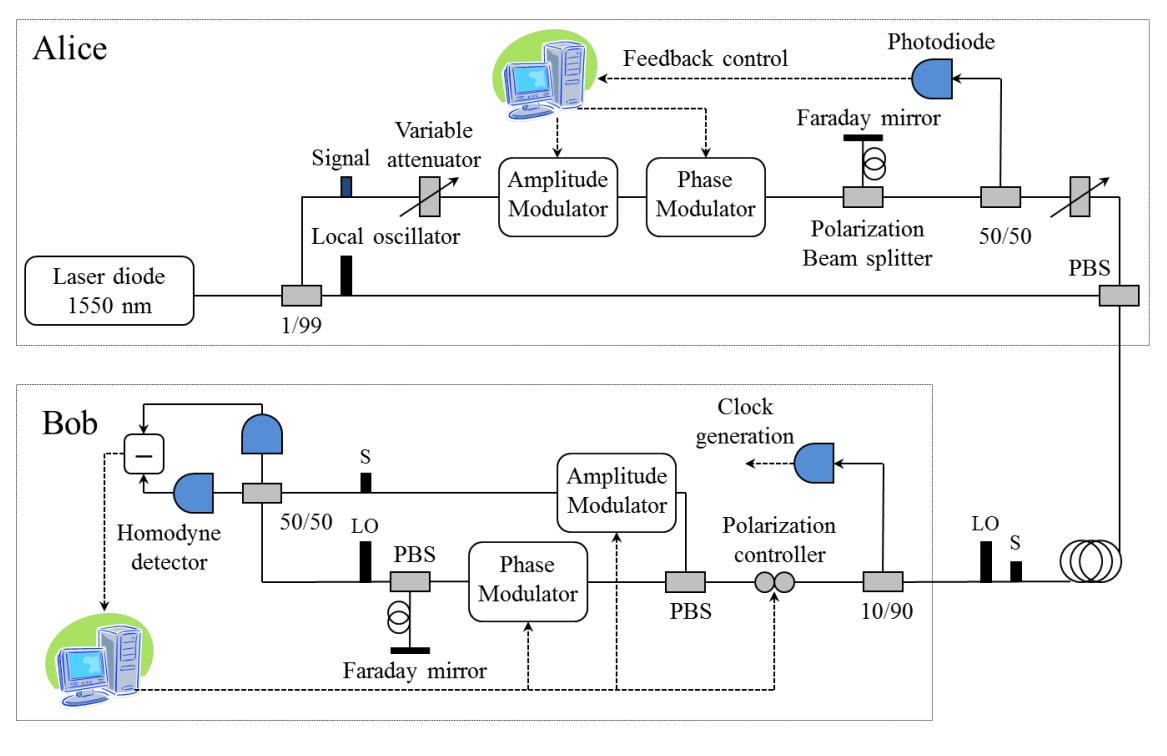
\includegraphics[width=\linewidth]{images/gg02 lit.png}
    \caption{Оптическая схема волоконной системы КРК-НП с гомодинным детектированием. Laser diode - лазерный диод, signal - сигнал, Local oscillator - локальный осциллятор, Variable attenuator - переменный аттенюатор, Amplitude modulator - амплитудный модулятор, Phase modulator - фазовый модулятор, Polarization beam splitter (PBS) - поляризационный делитель луча, Faraday mirror - Зеркало Фарадея, Photodiode - Фотодиод, Feedback control - управление обратной связью, Polarization controller - контроллер поляризации, Clock generation - генерация опорной частоты, Homodyne detector - гомодинный приемник.}
    \label{fig:gg02 lit}
\end{figure}
В этой схеме сигнал и опорная фаза (или локальный осциллятор), необходимые для выполнения когерентного обнаружения, генерируются источником лазерного диода в месте нахождения Алисы. Сигнал модулируется по амплитуде и фазе в соответствии с гауссовским распределением, как того требует протокол, а затем ослабляется на подходящем уровне дисперсии модуляции. Он также мультиплексируется по времени и по поляризации с локальным осциллятором перед входом в квантовый канал. На месте Боба два сигнала демультиплексируются с помощью линии задержки и поляризационного делителя луча и накладываются во времени для интерференции на ограниченный шумами сбалансированный импульсный гомодинный детектор. Квадратурная селекция, требуемая протоколом GG02, выполняется фазовым модулятором, помещенным в тракт локального генератора. Установка дополнена несколькими активными элементами обратной связи и управления, которые обеспечивают необходимые условия синхронизации и стабильности для выполнения квантового распределения ключей. 
Описанная система реализует первую часть, а именно (1) распределение и измерение состояния, полного протокола GG02, описанного в разделе \ref{GG02 exp lit}; остальные части постобработки, а именно 2 согласование ошибок, 3 оценка параметров и 4 усиление конфиденциальности, и, в частности, первые две, требуют сложных вычислительных алгоритмов. Первоначальная реализация оптической установки на рисунке \ref{fig:gg02 lit} использовалась в европейской сети SECOQC QKD, которая была развернута по проложенным оптическим волокнам и объединяла различные технологии КРК. Она также использовалась в полевых испытаниях линии связи точка-точка с классическим симметричным шифрованием и быстрым обновлением ключей, обеспечиваемым квантовым слоем, которые продемонстрировали надежность работы системы КРК-НП в течение длительного периода времени в условиях серверной. Эти реализации, а также некоторые другие, были пригодны для защиты коммуникаций в сетях городского масштаба (с расстоянием до 25 км) с высокими требованиями к скорости передачи данных. Хотя существует несколько интересных применений экспериментов на коротких расстояниях, с точки зрения квантовых информационных сетей важно иметь возможность увеличить расстояние связи за этот предел. В реализациях дискретно-переменного КРК ограничение по расстоянию в основном определяется характеристиками однофотонных детекторов, в частности, их темновыми отсчетами. В КРК-НП ограничение дальности было связано с эффективностью сложных методов постобработки. Хотя это уже не так, полезно понять причину этого ограничения: эффективное согласование коррелированных гауссовских переменных на самом деле затруднено, особенно при низких отношениях сигнал/шум (SNR), которые присущи экспериментам на больших расстояниях, что снижает коэффициент эффективность сверки. 
Помимо исправления ошибок, процедура оценки параметров также имеет решающее значение для извлечения секретного ключа на практике. Для оптической установки на рисунке \ref{fig:gg02 lit} соответствующими экспериментальными параметрами являются дисперсия модуляции Алисы $V_A$, коэффициент пропускания канала T и избыточный шум $\xi$, который представляет собой шум, добавляемый каналом сверх основного шума выстрела, и соответствует обычному коэффициенту ошибок квантового бита, встречающемуся в дискретно-переменных реализациях КРК. Как $V_A$, так и $\xi$ обычно выражаются в единицах дробового шума. Параметр $V_A$ подстраивается в реальном времени, чтобы в любой момент времени быть как можно ближе к SNR, соответствующему порогу доступного кода с исправлением ошибок, в то время как параметры T и $\xi$ должны оцениваться в реальном времени путем случайного раскрытия части ключа. Два дополнительных экспериментальных параметра, которые используются для вычисления оценки секретной информации, которая может быть извлечена из общих данных, - это скорость электронного шума и эффективность $\eta$ обнаружения гомодина. В так называемом реалистичном сценарии КРК-НП предполагается, что эти параметры недоступны для Евы и измеряются в ходе безопасной процедуры калибровки, которая проводится перед развертыванием системы. Однако в общем случае эти параметры могут быть доступны Еве. Процедура оценки параметров позволяет вычислить границы для информации подслушивающего лица, принимая во внимание неопределенность калиброванных значений.

\subsection{Протокол квантового распределения ключа с использованием модуляции Гаусса и локальным осциллятором, сгенерированным на приемной стороне}\label{sec:ch1/sect4/subsec2} %Generating the local oscillator locally in continuous-variable quantum key
%distribution based on coherent detection
Как протоколы КРК на дискретных переменных  (КРК-ДП) , основанные на обнаружении одиночных фотонов \cite{bennett1984,ekert1991}, так и протоколы КРК на непрерывных переменных (КРК-НП), основанные на когерентном детектировании \cite{ralph1999,hillery2000,grosshans2002} были продемонстрированы как жизнеспособные решения на практике. Одним из известных протоколов КРК-НП является протокол когерентного состояния с гауссовской модуляцией (ГМКС) \cite{grosshans2002}, который был продемонстрирован на 80-километровой оптоволоконной  линии связи \cite{jouguet2013a}. Одним из важных преимуществ ГМКС КРК  является его устойчивость к некогерентному фоновому шуму. Сильный локальный осциллятор (ЛО), используемый в когерентном обнаружении, также действует как естественный и чрезвычайно селективный фильтр, который может эффективно подавлять шумовые фотоны. Эта внутренняя функция фильтрации делает КРК-НП привлекательным решением для безопасного распределения ключей по зашумленному каналу, таком как освещенное волокно в обычной оптоволоконной оптической сети \cite{kumar2015} или оптической линии связи в свободном пространстве \cite{heim2014}.
Однако все существующие реализации КРК-НП основанные на когерентном детектировании, имеют серьезный недостаток: для уменьшения фазового шума как сигнал, так и ЛО генерируются одним и тем же лазером и распространяются по небезопасному квантовому каналу \cite{grosshans2002, jouguet2013a, heim2014} 1. Такая схема имеет несколько ограничений. Во-первых, она позволяет Еве получить доступ как к квантовому сигналу, так и к ЛО. Ева может проводить сложные атаки, манипулируя ЛО, что было продемонстрировано в недавних исследованиях \cite{ma2013, huang2013,jouguet2013}. Во-вторых, Передача сильного ЛО по каналу с потерями может резко снизить эффективность КРК в некоторых приложениях. Например, для достижения когерентного обнаружения с ограничением по дробовому шуму необходимое число фотонов в ЛО обычно превышает $10^8$ фотонов на импульс на стороне приемника. При частоте повторения импульсов 1 ГГц и потерях в канале 20 дБ, требуемая мощность ЛО на входе квантового канала составляет около 1,2 Вт (на длине волны 1550 нм). Если оптическое волокно используется в качестве квантового канала, шумовые фотоны, генерируемые сильным ЛО внутри оптического волокна, могут значительно снизить эффективность КРК и пропускную способность мультиплексирования. В-третьих, ЛО обычно на 7 или 8 порядков ярче, чем квантовый сигнал, поэтому требуются сложные схемы мультиплексирования и демультиплексирования для эффективного отделения ЛО от квантового сигнала на стороне приемника.
В КРК-НП желательно генерировать ЛО 'локально', используя независимый лазерный источник на стороне приемника. К сожалению, такая схема никогда не была реализована на практике. Основная проблема заключается в том, как эффективно установить надежную фазовую привязку между Алисой и Бобом. Хотя в классической когерентной связи были разработаны различные методы, такие как восстановление несущей \cite{ip2007}, оптическая фазовая автоподстройка частоты \cite{ma2013}, и оптическая инжекционная фазовая подстройка частоты \cite{fice2011}, были разработаны для классической когерентной связи, но эти методы не подходят для КРК, где квантовый сигнал крайне слаб, а допустимый фазовый шум мал.
Кроме того, чтобы предотвратить манипуляции Евы с ЛО, лазер ЛО должен быть изолирован от внешнего мира как оптически, так и электрически.
В этой статье решается вышеупомянутая давно нерешенная проблема, предложив и продемонстрировав схему восстановления данных с помощью пилота схема восстановления данных с обратной связью, которая обеспечивает надежное когерентное обнаружение с использованием "локально" генерируемого ЛО.
Эта схема основана на наблюдении, что в ГМКС КРК, Бобу не нужно выполнять измерение в "правильном базисе". Фактически, Боб может выполнить измерение в произвольно повернутом базисе, поскольку при условии, что информация о базисе (фазовый эталон) если информация о базисе (фазовый эталон) доступна после измерения. Имея эту информацию  после измерения, Алиса или Боб могут вращать имеющиеся данные и генерировать коррелированные данные с другими. 
\subsubsection{Экспериментальная реализация протокола КРК на непрерывных переменных с модуляцией Гаусса.}
\begin{figure}
    \centering
    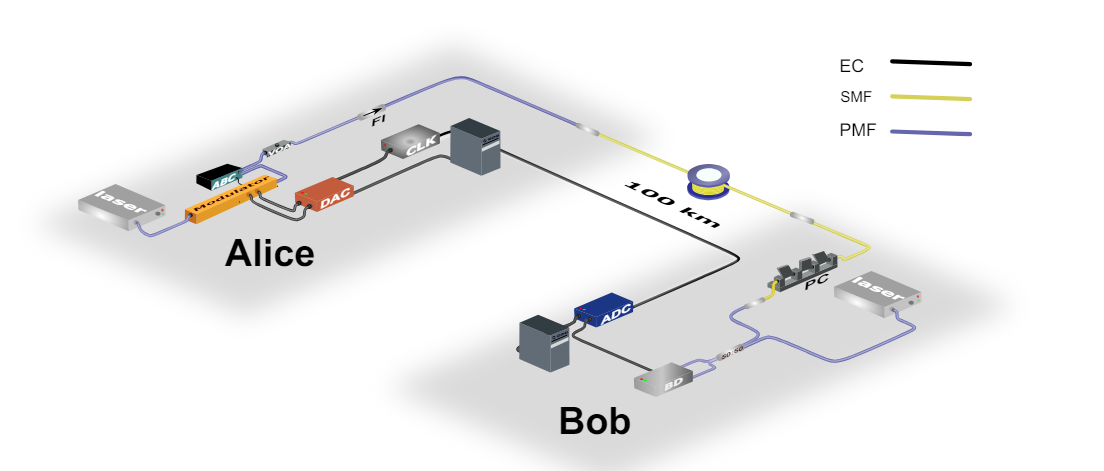
\includegraphics[width=0.9\linewidth]{images/QKD CV LLO.png}
    \caption{Станция Алисы состоит из непрерывного (CW) лазера, работающего на длине волны 1550 нм, синфазного и квадратурного (IQ) модулятора с автоматическим регулятором смещения (ABC) для получения когерентных состояний на боковых частотах. A Для управления IQ-модулятором использовался цифро-аналоговый преобразователь (ЦАП) с разрешением 16 бит и частотой дискретизации 1 Гвыб/с. Переменный оптический аттенюатор (VOA) использовался после IQ-модулятора для регулировки дисперсии модуляции квантового сигнала. Изолятор Фарадея (ФИ), направление которого указано стрелкой, используется перед 100-километровым оптоволоконным каналом со сверхнизкими потерями, который представляет собой квантовый канал. Станция Боба состоит из поляризационного контроллера (ПК) для настройки поляризации входящего сигнала и сбалансированного светоделителя для наложения этого сигнала на локальный осциллятор, генерируемый другим CW-лазером (разблокированным/свободно работающим по отношению к лазеру Алисы). Сигнал был обнаружен и оцифрован с помощью сбалансированного детектора (BD), а затем аналого-цифрового преобразователя (АЦП) с частотой дискретизации 1 Гвыб/с.}
    \label{fig:CV QKD ЛЛО lit}
\end{figure}
На рисунке \ref{fig:CV QKD ЛЛО lit} показана оптическая схема  системы КРК-НП с "локальным" локальным осциллятором (ЛЛО) \cite{hajomer2024}, основанной на протоколе когерентного состояния с гауссовской модуляцией. У отправителя, Алисы, в качестве оптического носителя использовался непрерывный лазер (CW) с узкой шириной линии $\approx$ 100 Гц, работающий на длине волны 1550 нм. Когерентные состояния готовились путем модуляции КВ-лазера с помощью синфазно-амплитудного (IQ) модулятора, управляемого 16-битным цифро-аналоговым преобразователем (ЦАП) с двумя каналами, работающими с частотой дискретизации 1 Гвыб/с. IQ-модулятор работал в однополосном режиме, управляя напряжениями смещения постоянного тока (DC) с помощью автоматического регулятора смещения (ABC). После IQ-модулятора был установлен переменный оптический аттенюатор (VOA) для регулировки дисперсии модуляции теплового состояния. На выходе отправителя был добавлен изолятор Фарадея, чтобы избежать обратных отражений от канала и атак "троянского коня". Сигнал передавался по квантовому каналу, изготовленному из коммерческого волокна с ультранизкими потерями (TeraWave SCUBA 150 Ocean Optical Fiber). Затухание волокна составляет 0,146 дБ/км на длине волны 1550 нм. Общие потери в нашем 100-километровом оптоволоконном канале составили 15,4 дБ из-за разницы диаметров модового поля между соединением волокна SMF-28 и SCUBA 150.
В приемнике Боба для измерения квантового состояния использовалось радиочастотное (РЧ) гетеродинное детектирование. Для этого в качестве ЛЛО использовался другой CW-лазер, свободно работающий по отношению к лазеру Алисы. Разница частот между
лазерами Алисы и Боба составляла $\approx$ 230 МГц. Затем поляризация квантового сигнала была настроена так, чтобы соответствовать поляризации ЛЛО с помощью регулятора поляризации. Затем квантовый сигнал и ЛЛО были объединены на сбалансированном светоделителе,
затем самодельный сбалансированный детектор с полосой пропускания
$\approx$ 365 МГц для обнаружения интерференционной картины. Наконец, обнаруженный сигнал оцифровывался с помощью 16-битного аналого-цифрового преобразователя (АЦП) с частотой дискретизации 1 Гвыб/с и записывался для автономной цифровой обработки сигнала. АЦП и ЦАП были синхронизированы с помощью опорного генератора (CLK) с частотой 10 МГц.
Время измерения делилось на кадры, каждый из которых содержал $10^7$ выборок АЦП. Три измерения проводились автономно: измерение квантового сигнала, измерение вакуумного шума (лазер Алисы выключен, лазер Боба включен) и измерение электронного шума (лазер Алисы выключен, лазер Боба выключен). Выигрыш вакуумного шума по сравнению с электронным составил $\approx$ 15 дБ в полосе частот квантового сигнала. Чтобы откалибровать $V_{mod}$ теплового состояния, проводились измерения "спина к спине" (B2B), в которых Алиса и Боб были соединены через короткий волоконный патч-корд, а VOA был тонко настроена для установки различных значений $V_{mod}$.
\newline Передача данных на большие расстояния является ключевым требованием для широкомасштабного развертывания и интеграции КРК в существующие телекоммуникационные сети. КРК-НП естественным образом подходит для такой интеграции. Однако безопасная и практичная конфигурация системы (ЛЛО КРК-НП) сталкивается с ограничениями по дальности передачи из-за фазового
фазового шума лазеров. В данной работе демонстрируется  возможность передачи данных на большие расстояния ЛЛО КРК-НП по оптоволоконному каналу длиной 100 км . Этот рекордный эксперимент стал возможен благодаря использованию машинного обучения для компенсации фазового шума и оптимизации модуляции для согласования информации и избыточного шума одновременно.

\section{Фазовый шум в системах квантового распределения ключа}\label{sec:ch1/sect5}
Фазовый шум в системах квантового распределения ключа является одним из факторов, которые ограничивают скорость выработки секретного ключа. В то время, как этот эффект практически не влияет на протоколы, построенных на дискретных переменных, но этот эффект является критическим для протоколов на непрерывных переменных, как и для протоколов, основанных на "полях близнецах" и с недоверенным приемным узлом. В случае этих протоколов происходит интерференция либо нескольких когерентных состояний между собой, либо между когерентным состоянием и локальным осциллятором. В обоих случаях происходит измерение, которое будет зависеть от разности фаз между взаимодействующими компонентами излучения. И в случае наличия дополнительного фазового шума, результат этой интерференции будет абсолютно случайным, независимым от закодированных состояний Алисой и Бобом. В этом случае ключ не будет сгенерирован. Поэтому данный шум необходимо компенсировать различными методами.
\newline Избыточный шум в системах КРК может быть обусловлен различными источниками: дискретизация, модуляция, относительный шум интенсивности (RIN), рассеяние Рамана и  остаточный фазовый шум (RPN). Предполагается, что эти источники шума статистически независимы и поэтому общий избыточный фазовый шум может быть представлен в виде суммы независимых величин
\begin{equation}
    \zeta = \zeta_{RIN} + \zeta_{mod} + \zeta_{quant} + \zeta_{Ramman} + \zeta_{RPN} + K
\end{equation}\label{eq:noise lit}
Среди этих источников шума, остаточный фазовый шум (ОФШ), определяется как распределение разности между реальной фазой квантового сигнала и измеренной фазой принятого сигнала, является главным источником избыточного шума в системах КРК-НП ЛЛО. В случае гауссово-модулированного протокола на когерентных состояния, избыточный шум, связанный с ОФШ на приемной стороне определяется как 
\begin{equation}
    \zeta_{ОФШ} = 2TV_{mod}(1-e^\frac{-V_{RPN}}{2}) 
\end{equation}\label{eq: noise phase llo lit}, где T - пропускание, включающее в себя квантовый канал и эффективность детектора, $V_{mod}$ - распределение модуляции, т.е. распределение ансамбля когерентных состояний и $V_{ОФШ}$ - распределение остаточного фазового шума.
Исходя из выражения \ref{eq: noise phase llo lit}, доступно два варианта уменьшение фазового шума в КРК-НП с ЛЛО: работа системы при низкой дисперсии модуляции или минимизация ОФШ. Хотя первый вариант практичен и прост в реализации, он требует тщательной оптимизации $V_{mod}$ из-за зависимости скорости выработки секретного ключа от дисперсии модуляции. В частности, от дисперсии модуляции зависят как взаимная информация, так и эффективность согласования информации.
Для уменьшения ОФШ требуется эффективная оценка фазы. В настоящее время стандартный подход заключается в использовании пилотных методов для оценки относительной фазы между непрерывно излучающими лазерами  передатчика и приемника. Качество оценки фазы сильно зависит от отношения сигнал/шум (SNR) пилотных сигналов, реализуемых с помощью одночастотных тонов или обучающих символов, передаваемых вместе с квантовым сигналом. Однако эти методы ограничены потерями в канале, которые увеличиваются с расстоянием, и необходимостью в маломощном пилотном сигнале для уменьшения перекрестных помех квантовому сигналу.

\subsection{Методы борьбы с фазовым шумом в системах квантового распределения ключа}\label{sec:ch1/sect5/subsec1}
В ходе развития технологии квантового распределения ключа были разработаны несколько методов компенсации фазовых искажений с целью улучшения характеристик конечных систем. Существует несколько способов реализации компенсаций фазовых искажений: восстановление фазы несущей частоты, пилотные импульсы и реализация обратной связи в виде оптической инжекции или оптической фазовой автоподстройки частоты. Данные методы обладают как своими преимуществами, так и недостатками. Данный раздел посвящен рассмотрению принципов работы данных методов компенсации фазовых искажений. 
\subsubsection{Пилотные импульсы}Первым из методов восстановления стали так называемые пилотные импульсы \cite{wang2020}. Их суть заключается в том, что к квантовым состояниям мультиплексируется дополнительный классический сигнал, который является опорным для измерения фазового шума при прохождении квантового канала. После прохождения этими сигналов квантового канала, они попадают на схему демультиплексирования и разделяются. На балансном детекторе происходит измерение фазы и пилотного импульса, и квантового сигнала. Так как эти оба сигнала распространялись по одному и тому же каналу, а также были излучены одним и тем же источником, то их фазовые шумы являются скоррелированными. В результате измерения фазы  пилотного импульса, можно вносить корректировки измеренного фазового набега в квантовом сигнале на этапе постобработки. 
\newline Однако данный метод усложняет приемный модуль за счет необходимости дополнительной системы демультиплексирования, а также увеличивает шум, связанный с рассеянием, так как передаваемый  пилотный импульс должен быть достаточно мощным для точных измерений.
\subsubsection{Оптическая фазовая автоподстройка частоты}
Другим же методом подстройки фазы двух источников излучения является оптическая фазовая автоподстройка частоты или ОФАПЧ (OPLL) \cite{khaksar2023}. В этом случае, два лазера сбиваются на фотоприемнике. Их разностная частота подстраивается так, чтобы она сравнялась с опорной частотой генератора, относительно которой будет подстраиваться фаза излучения. 
В качестве источника опорной частоты может выступать термостатированный кварцевый генератор. Эти частоты сбиваются на смесителе для формирования сигнала ошибки. Этот сигнал ошибки передается на PID контроллер температуры лазера для управления его длиной волны до тех пор, пока этот сигнал ошибки не станет меньше заданного значения.
Из плюсов данной реализации можно выделить ее точность и скорость работы. К недостаткам можно отнести сложность исполнения и необходимость точной подстройки и стабилизации температур и токов лазеров.

\section{Известные атаки злоумышленника на источники лазерного излучения}\label{sec:ch1/sect7}
Секретность распределенного ключа в системах квантового распределения базируется на теоретических доказательствах секретности, в которых допускается, что злоумышленник (Ева) может сделать все, что не запрещено законами квантовой физики. Однако, несовершенства технической реализации систем КРК позволяют Еве их использовать для доступа к части секретного ключа. Среди таких атак выделяется атаки на источник лазерного излучения в системе КРК. Этот тип атак позволяет увеличить мощность, излучаемую лазером, установленным в Алисе, и таким образом увеличить среднее число фотонов. Этот эффект позволяет применять атаку с расщеплением числа фотонов эффективнее и получать доступ к части секретного ключа. 
\newline Другой же тип атаки направлен непосредственно на Локальный осциллятор в системе КРК-НП для изменения времени начала синхронизации
\subsection{Атака "засевом" лазерным излучением}\label{sec:ch1/sect7/subsec1}
Первоначально атаки злоумышленника были нацелены на приемную часть, а именно на детектор одиночных фотонов \cite{makarov2009, sajeed2020, chistiakov2019, qian2018}. В результате этой атаки злоумышленник имеет возможность "навязывать" секретный ключ легитимным пользователям \cite{lydersen2010}. 
В дальнейшем  появились атаки на модуляторы - атака "троянским конем". Такое воздействие позволяет узнать о выборе базиса легитимными пользователями и иметь доступ к секретному ключу за счет зондирования фазового модулятора излучением, сильно отличающимся по длине волны от той, что используют Алиса и Боб \cite{jain2014,a-etsi2021,gisin2006}.
Но существует и атака на источник излучения из состава системы квантового распределения ключей - атака "засевом" лазерным излучением \cite{huang2019,lovic2023}. Одним из главных условий секретности распределенного ключа в системах КРК является предположение, что интенсивность квантовых состояний, передаваемых Алисой, в среднем меньше 1 фотона на импульс.
Однако атака "засевом" позволяет нарушить это предположение. Стратегия этой атаки заключается в следующем. Злоумышленник использует свое мощное излучение на близкой длине волны и посылает его в оптическую схему Алисы.
В результате мощность, претерпевшая затухание из-за прохождения оптических элементов, попадает в резонатор лазера Алисы. Инжектированные таким образом носители увеличивают выходную мощность вынужденного излучения Алисы. 
Под действием излучения увеличивается и энергия импульса, и непрерывная мощность. В результате этого увеличивается излучаемое число фотонов Алисой. Этот эффект позволяет злоумышленнику либо производить различение состояний-ловушек в протоколах с их реализацией или же проводить успешнее атаку с разделением числа фотонов, тем самым получая доступ к секретному ключу. 
Еще одним эффектом, который негативно сказывается на секретности распределяемого ключа, является возможность злоумышленника вносить корреляции в излучение Алисы. Это происходит также с помощью атаки "засевом" лазерным излучением.
Однако создание корреляций происходит с помощью зондирования импульсным излучением, а не непрерывным как в других работах. Интерференционная картина импульсов злоумышленника и Алисы будут скоррелированны и для внесения этой корреляции не требуется большой мощности - достаточно 1 нВт средней мощности. 
С ростом зондирующей мощности корреляции будут только возрастать, что позволит получить Еве также доступ к части секретного ключа.
\newline Таким образом, атака "засевом" лазерным излучения является серьезной угрозой стойкости систем КРК, которую необходимо учитывать и разрабатывать контрмеры для ее предотвращения. 

\subsection{Атака на мощность локального осциллятора в системах квантового распределения ключа на непрерывных переменных}\label{sec:ch1/sect7/subsec2}
Существующие системы квантового распределения ключей на непрерывных переменных используют один лазер для генерации квантовых состояний и локального осциллятора. Такой подход позволяет упростить конечную систему. 
Однако, у генерации ЛО на стороне передатчика есть несколько недостатков: снижение уровня сигнала ЛО при передаче по волокну в виду естественного затухания. Другой же недостаток данного подхода - уязвимость ЛО ко внешнему воздействию злоумышленника.
В работе \cite{jouguet2013, fan2023} описывается атака на ЛО в системе КРКНП. В доказательствах секретности не учитывается ЛО, хотя он, как классический сигнал, может быть без проблем перехвачен, измерен, усилен и отправлен снова в канал.
Локальный же осциллятор используется для оценки пропускания канала и оценки распределения шума детектора - дробового шума. Эта величина является критической для оценки секретности ключа. 
Стратегия злоумышленника заключается в следующем. Злоумышленник вносит затухание в начало локального осциллятор. Так как ЛО используется для генерации опорной частоты, то внесение затухания в ЛО вызывает задержку во времени при формировании опорной частоты.
Для выполнения успешной атаки Ева производит следующие действия
\begin{enumerate}
    \item Нарушитель, Ева, вводит аттенюатор, не разрушающий фазу излучения, в квантовый канал и применяет некоторое затухание $\alpha$ ($0\leq \alpha \leq 1)$ на часть $\nu (0 \leq \nu \leq 1)$ импульсов локального осциллятора для изменения их формы. Тактовая частота, формируемая для гомодинного детектирования, зависящая от этих импульсов, сдвигается на величину $\delta$.
    \item Ева вводит светоделитель в квантовый канал и для части $\mu (0 \leq \mu \leq 1)$ входящих импульсов выполняет измерение обеих квадратур и подготавливает подходящие квантовые состояния, когда как для части $1 -\mu$ сигнальных импульсов, применяется функция светоделителя. Это называется частичной атакой "перехват - пересылка". 
\end{enumerate} 
Когда Ева увеличивает часть $\mu$ сигнальных импульсов, для которых она выполняет атаку "перехват-пересылка", то она вносит больше шума, который снижает количество секретных бит ключа, которые Алиса и Боб могут извлечь из квантовой передачи.
Часть $\nu$ локального осциллятора, в которую вносится затухание, и само затухание $\alpha$ - это два параметра, которые выполняют одну и ту же функцию - масштабируют распределение измерений, выполненных Бобом, не изменяя границу его дробового шума. Это приводит к тому, что Алиса и Боб приходят к выводу о том, что в квантовый канал не было внесено дополнительного шума, зеленый график на рисунке \ref*{fig:CV_attack} и поэтому распределяют ключ без обнаружения Евы.

\begin{figure}
    \centering
    \includegraphics*[width=\linewidth]{CV_attack.png}
    \caption{График распределения шума гомодинного детектора без атаки (красный цвет) и под действием атаки (зеленый) на ЛО.}
    \label{fig:CV_attack}
\end{figure}
\subsection{Выводы по главе}\label{sec:ch1/sect8}
В данной главе рассматриваются основы технологии квантового распределения ключей. Рассмотрены подходы по созданию систем КРК на дискретных переменных по топологии "точка-точка", так и с недоверенным приемным узлом. Как альтернатива протоколам на дискретных переменных рассмотрены протоколы на непрерывных переменных. Продемонстрированы  различные подходы к реализации локального осциллятора в системах КРКНП. Показаны этапы протокола выработки битовых последовательностей для протоколов на дискретных переменных, так и на непрерывных.
Изучен вопрос атак на техническую реализацию систем квантового распределения ключей. Особенно акцентировано внимание на атаках на источники излучения в КРК. Все рассмотренные вопросы создают базовое понимание технологии КРК, которые необходимы для понимания последующих глав.           % Глава 1
\chapter{Система квантового распределения ключа на боковых частотах с применением обратной связи}\label{ch:ch2}
\renewcommand{\thefigure}{2.\arabic{figure}} % Plain numbering
\setcounter{figure}{0}                     % Reset if needed


\section{Система квантового распределения ключа на боковых частотах}\label{sec:ch2/sect9}
Одной из существующих реализаций систем квантового распределения ключа является реализация на боковых частотах, предложенная Юрием Тарасовичем Мазуренко \cite{gleim2016}. 
В отличии от других систем квантового распределения ключа, где лазерное излучение ослабляется до уровня мощности менее 1 фотона в импульсе, в системе квантового распределения ключа на боковых частотах (КРКБЧ) \cite{gleim2016} генерируются квантовые состояния на дополнительных оптических каналах, которые получаются в результате модулирования 
оптического лазерного излучения переменным электрическим сигналом с помощью электро-оптического модулятора на основе кристалла ниобата лития.
Такая реализация системы квантового распределения ключа дает преимущества в виде
\begin{enumerate}
    \item Устойчивость ко внешним воздействиям в виде колебаний волоконно-оптического тракта, которые изменяют поляризацию квантовых состояний случайным образом.
    \item Возможность реализации частотного мультиплексирования на одной оптической несущей частоте для повышения информационной емкости канала или для повышения его секретности за счет случайного выбора частоты для измерений квантовых состояний.
    \item Совместимость с текущими волоконно-оптическими линиями связи за счет применения стандартной элементной-компонентной базы. 
\end{enumerate}
Эти преимущества выделяют систему квантового распределения ключа на боковых частотах среди остальных.
\subsection*{Принцип работы системы КРКБЧ}
Установка КРКБЧ, изображенная на рисунке \ref{fig:krkbch} работает следующим образом. 
\begin{figure}
    \centering
    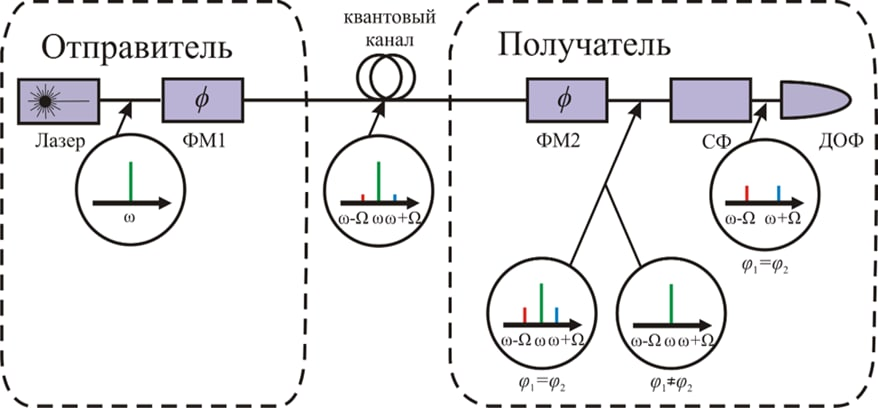
\includegraphics[width=\linewidth]{krkbch.jpg}
    \caption{Принципиальная схема установки системы квантового распределения ключей на боковых частотах.}
    \label{fig:krkbch} 
\end{figure}
Полупроводниковый лазер с рабочей длиной волны генерирует излучение на длине волны 1550 нм. Это излучение передается по волоконно-оптическому тракту с сохранением поляризации на фазовый модулятор.
На электрический же вход электо-оптического модулятора подается радиосигнал, сформированный генератором. В качестве генератора выступает I/Q генератор, который на выходе выдает частоту 4.8 ГГц с фазовым кодированием.
Эти фазовые сдвиги определяют какое квантовое состояние кодирует Алиса в свои состояния. Значения данных фазовых сдвигов соответствуют значениям {0, 90, 180, 270} градусов. 
В результате взаимодействия электрического и оптического сигнала внутри кристалла, на выходе модулятора в оптическом сигнале появляются дополнительные гармоники. Их частота будет равна $\omega - \Omega$ и $\omega + \Omega$, где $\omega$ - частота излучения лазера, $\Omega$ - частота модуляции.
Полученный в результате сигнал попадает на модулятор интенсивности на основе кристалла ниобата лития. Данное устройство создает импульсы из непрерывного излучения, сгенерированного лазером. Это необходимо для того, чтобы было возможно регулировать время прихода одиночного фотона на детектор одиночных фотонов, режим работы которого будет описан далее.
Приготовленные импульсы попадают на переменный оптический аттенюатор (ПОА), который вносит затухание в пришедший сигнал до такого уровня, что на боковых частотах должна быть мощность, которая соответствует среднему числу фотонов меньше единицы.
При этом на несущей частоте допускается использование мощности больше 1 фотона в среднем, так как сигнал на этой частоте не используется для распределения секретного ключа.
Сгенерированные квантовые состояния передаются в блок приемника по стандартной волоконно-оптической линии связи, построенной с помощью одномодового волокна. 
Пройдя ВОЛС сигнал попадает на блок приемника. 
При прохождении сигнала по такой линии связи, поляризация прошедшего состояния изменяется на случайную, что приводит к негативным последствиям. Чтобы нивелировать искажения поляризации устанавливается поляризационный светоделитель, который разделяет пришедший сигнал по поляризации на линейную и циркулярную, при этом линейная проходит без изменений, а циркулярная поворачивается так, чтобы она стала линейной. После этого сигнал попадает на два фазовых модулятора. С помощью этих модуляторов происходит повторная модуляция, идентичная модуляции на стороне передатчика. В результате этого на боковых частотах будет наблюдаться интерференция, результат которой зависит от разности фаз между передатчиком и приемником. После повторной модуляции необходимо удалить несущую частоту, так как она не используется для генерации ключей. Для этого после поляризационного объединителя устанавливается спектральный фильтр на основе волоконной Брэгговской решетки.
В результате после фильтра остаются только боковые частоты, которые несут в себе информацию о квантовых состояниях. Этот сигнал регистрируется детектором одиночных фотонов, который отправляет срабатывания в программируемую логическую интегрируемую схему, где формируется последовательность бит, называемая сырым ключом. После формирования сырого ключа происходит общение по служебному каналу между приемником и передатчиком по служебному каналу для процедур просеивания ключа и исправления ошибок. После исправления ошибок начинается операция усиления секретности, в результате которой формируется секретный ключ.
\section{Метод оптической инжекции}\label{sec:ch2/sect1}
Для систем квантового распределения ключа необходимы стабильные источники излучения с фиксированной длиной волны и без нелинейных эффектов в виде чирпа \cite{yuan2016, roberts2018}. Некачественные источники лазерного излучения приводят к нарушению интерференционной  картины в случае протоколов MDI \cite{comandar2016} или же снижению скорости генерации секретного ключа и уменьшения дальности его передачи в протоколах BB84 с применением состояний ловушек \cite{xie2019}. Одним из активно развивающихся решений этой проблемы является метод фазовой синхронизации с помощью оптической инжекции \cite{liu2020}. 
\newline Полупроводниковые лазеры  на основе кристалла InGaAs имеют выходное зеркало, которое пропускает больше 50\% излучения. Благодаря такому коэффициенту пропускания, такие лазеры подвержены внешнему оптическому воздействию, которое зачастую является нежелательным из-за возможного образования паразитной обратной связи. Однако эту прозрачность можно использовать во благо для реализации оптической инжекции. Этот метод предлагает использование второго лазера, излучение которого попадает в резонатор другого лазера, образуя пару ведущий - ведомый \cite{shakhovoy2024}. В результат этого выходное излучение ведомого лазера меняется под действием излучения ведущего источника. К плюсам метода оптической инжекции можно отнести следующее
\begin{enumerate}
    \item Применение оптической инжекции улучшает форму спектра выходного излучения, уменьшая дополнительные гармоники.
    \item Уменьшает возникающие в кристалле нелинейные процессы, негативно влияющие на частотный состав выходного излучения
    \item Улучшает форму выходных импульсов за счет подавления релаксационных колебаний и стабилизации выходной частоты
    \item Стабилизация амплитуды и длительности импульсов
\end{enumerate}
Данные эффекты положительно сказываются на качестве выходного излучения и, как следствие, положительно влияют на характеристики систем квантового распределения ключей, в которых они используются.
\subsection{Математическая модель оптической инжекции}
Система уравнений описывающих излучение ведомого лазера:
\begin{equation}\label{eq:systemForMaster}
	\begin{split}
		\dot{Q}^{\text{м}} &= (G^{\text{м}} - 1)\frac{Q^{\text{м}}}{{{\tau_{\text{ф}}^{\text{м}}}}}+ C_{\text{сп}}^{\text{м}} R_{\text{сп}}^{\text{м}} +F_Q^{\text{м}}, \\ 
		\dot{\varphi}^{\text{м}} &= \frac{\alpha^{\text{м}} }{{2{\tau_{\text{ф}}^{\text{м}}}}}(G_{\text{лин}}^{\text{м}} - 1)+F_\varphi^{\text{м}},\\
		\dot{N} ^{\text{м}} &= \frac{I^{\text{м}}}{e} - \frac{N^{\text{м}}}{{{\tau _e^{\text{м}}}}} - \frac{{G^{\text{м}}Q^{\text{м}}}}{{\Gamma^{\text{м}} {\tau_{\text{ф}}^{\text{м}}}}}+F_N^{\text{м}},	
	\end{split}
\end{equation}
и связанную систему для ведомого лазера:
\begin{equation}\label{eq:systemForSlave}
	\boxed{	\begin{split}
			\dot{Q} &= (G - 1)\frac{Q}{{{\tau_{\text{ф}}}}}+ C_{\text{сп}} R_{\text{сп}}+ \\
			&
			+ 2{\kappa_{\text{и}}}\sqrt {Q^{\text{м}}Q} \cos (\Delta \omega_{\text{и}} t + {\varphi ^{\text{м}}} - \varphi )+F_Q, \\ 
			\dot{\varphi} &= \frac{\alpha }{{2{\tau_{\text{ф}}}}}(G_{\text{лин}} - 1)+ \\
			&+ {\kappa_{\text{и}}}\sqrt {\frac{{Q^{\text{м}}}}{Q}} \sin (\Delta \omega_{\text{и}} t + {\varphi^{\text{м}}} - \varphi )+F_\varphi,\\
			\dot{N} &= \frac{I}{e} - \frac{N}{{{\tau _e}}} - \frac{{GQ}}{{\Gamma {\tau_{\text{ф}}}}}+F_N,
	\end{split}}
\end{equation}
где члены $C_{\text{сп}}^{\text{м}}R_{\text{сп}}^{\text{м}}$ и $C_{\text{сп}}R_{\text{сп}}$ описывают вклад спонтанного излучения, а $F_Q^{\text{м}} $, $F_\varphi^{\text{м}}$, $F_N^{\text{м}}$ и $F_Q$, $F_\varphi$, $F_N$ -- ланжевеновские силы для ведущего и ведомого лазеров соответственно.
\section{Определение частотного диапазона фазовой синхронизации двух когерентных источников излучения}\label{sec:ch2/sect2}
При методе оптической инжекции необходимо учитывать то, что два лазера необходимо настроить таким образом, чтобы их излучение синхронизировалось по фазе. Для этого необходимо учитывать то, что существует полоса синхронизации, которая определяется как 
\begin{equation}\label{eq:DbigOmega}
	\Delta \Omega=\Delta \omega_{\text{синх}} \sin(\varphi_{\text{синх}}-\psi),
\end{equation}
где $\Delta \omega_{\text{синх}}$ определяется как
\begin{equation}\label{eq:lockingBandwidth}
	\Delta \omega_{\text{синх}} = z\sqrt{1+\alpha^2(1+2\gamma_Q Q_\text{с})},
\end{equation}
и где мы ввели обозначение
\begin{equation}\label{eq:z}
	z=\kappa_{\text{и}}\sqrt{Q^{\text{м}}_\text{с}/Q_\text{с}}.
\end{equation}

Уравнение \eqref{eq:DbigOmega} накладывает первое ограничение на полосу синхронизации, которое можно записать следующим образом:
\begin{equation}\label{eq:symLockingBandwidth}
	\lvert \Delta \Omega \rvert \le\Delta \omega_{\text{синх}}.
\end{equation}
выражение \ref{eq:symLockingBandwidth} показывает, что необходимо подбирать частоты и мощности ведущего и ведомого лазера для их синхронизации. 
\newline Для этого используются исследуемые лазеры и оптический анализатор спектра. У ведущего лазера изменяется длина волны за счет изменения температуры кристалла, контролируемой управляющей электроникой через элемент Пельтье. Излучение лазера ведомого подключается через оптический циркулятор с сохранением поляризации для минимизации потерь в волокне. Второй вход циркулятора же подключен к волоконному выводу лазера-ведомого, чтобы излучение из лазера-ведущего входило внутрь резонатора. Выходное излучение лазера-ведомого подается на второй выход циркулятора и проходит в третий его порт, где устанавливается оптический анализатор спектра, который измеряет характеристики пришедшего излучения. В случае синхронизации, на анализаторе спектра возникает только одна длина волны лазера без изменений. Однако в случае разницы длин волн слишком большой, то будет наблюдаться несколько гармоник излучения, которые соответствуют длинам волн лазера-ведомого и лазера-ведущего. При некоторой комбинации длин волн, может также наблюдаться генерация нелинейных гармоник сигнала, сигнализирующих о том, что лазеры находятся в зоне нестабильной синхронизации. 
Таким образом подбирается оптимальное соотношение длин волн лазеров. Для дальнейшего изучения диапазона возможно использование перестраиваемого аттенюатора в волоконном тракте лазера-ведущего для изменения соотношения мощностей лазера-ведущего и лазера-ведомого.
\section{Изменение длины волны излучения локального осциллятора под действием внешнего излучения.}\label{sec:ch2/sect7}
Для измерения влияния оптической инжекции на длину волны лазера локального осциллятора, установленного на приемной стороне, необходимо измерить длину волны под действием оптической инжекции и без нее. 
Для этого была собрана оптическая схема состоящая из
\begin{enumerate}
    \item Лазер-ведущий, установленный в передатчике
    \item Лазер-ведомый, установленный в приемнике
    \item Оптический анализатор спектра Yokogawa AQ6370D
    \item Оптический циркулятор с сохранением поляризации
\end{enumerate}
Излучение лазера-ведущего подается на первый порт оптического циркулятора, оно проходит во второй порт циркулятора, где подключен лазер-ведомый. Его же излучение проходит в 3 порт циркулятора и попадает на спектроанализатор.
Производится измерение длин волн лазеров ведущего и ведомого без воздействия внешнего излучения. Результаты этих измерений отображены на рисунке \ref*{fig:spectrums_injection}
Измеренные длины волн лазеров - длина волны лазера-ведущего 1549.964 нм, длина волны лазера-ведомого без действия внешнего излучения - 1549.808 нм. Под действием же излучения от лазера-ведущего длина волны лазера-ведомого становится 1549.949 нм. То есть практически идеально совпадает с длиной волны лазера-ведущего.
\begin{figure}
    \centering
    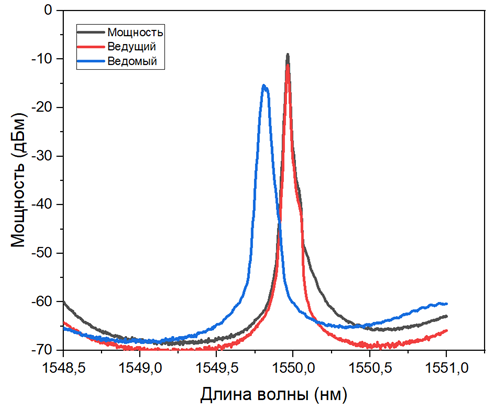
\includegraphics[width=\linewidth]{spectum_laser_injection.png}
    \caption*{Спектры лазерного излучения. Красным цветом отображен спектр излучения лазера-ведущего, синим - лазера-ведомого, а черным - лазера-ведомого под действием лазера-ведущего}
    \label{fig:spectrums_injection}
\end{figure}
Данный эффект позволяет убрать промежуточные частоты, которые бы возникали при использовании двух разных источников излучения, что упрощает постобработку, а также снижает фазовый шум, т.к. фазы лазеров будут скоррелированы и будет требоваться корректировка только из-за прохождения квантовыми состояния волоконно-оптической линии связи.
\section{Математическая модель гетеродинного детектирования для системы КРК на боковых частотах с применением обратной связи.}\label{sec:ch2/sect3}
Излучение лазера может быть представлено следующим образом:
\begin{align}
F(t) = A_0 * \sin(\omega_0 t + \phi_0),
\end{align}
где $A_0$ -- амплитуда сигнала, $\omega_0$ -- частота лазерного излучения, $\phi_0$ -- начальная фаза излучения.
Модулирующий сигнал:
\begin{align}
S(t) = (1+ m\sin(\Omega t  + \phi (t))),
\end{align} 
где $m$ -- индекс модуляции, $\Omega$ -- частота модуляции, $\phi (t)$ -- вносимая модуляция.

Лазерное излучение после модуляции выглядит следующим образом:
\begin{align}
\label{eq:laser}
F_s(t) &= F(t) * S(t) = A_0 * \sin(\omega_0 t + \phi_0) + \frac{A_0 * m}{2} * (\cos((\omega_0 + \Omega)t + (\phi_0 + \phi (t))) - \notag \\
&- \frac{A_0 * m}{2} * (\cos((\omega_0 - \Omega)t + (\phi_0 - \phi (t))),
\end{align}

Результат квадратичного детектирования сигнала, полученного в выражении~\eqref{eq:laser} будет выглядеть следующим образом:
\begin{align}
F_d(t) &= F(t)^2 * S(t)^2 = (A_0 * \sin (\omega_0 t + \phi_0))^2 * (1 + m*\sin (\Omega t + \phi_0 + \phi (t))^2=\notag \\
&= \frac{1}{8}\bigg \{4A_0^2 + 2A_0^2 *m^2 - 4A_0^2\cos(2\omega t + 2\phi_0) - 2A_0^2*m^2\cos(2\omega t + 2\phi_0) - \notag \\ & - 2A_0^2*m^2\cos(2\Omega t + 2\phi(t))  + A_0^2*m^2\cos(2\omega t - 2\Omega t + 2\phi_0 - 2\phi(t)) + \notag \\ & + A_0^2*m^2\cos(2\omega t + 2\Omega t + 2\phi_0 + 2\phi(t)) + 8A_0^2m\sin(\Omega t + 2\phi(t)) -\notag \\ & + 4A_0^2m\sin(2\omega t - \Omega t +2\phi_0 - \phi(t)) - 4A_0^2m\sin(2\omega t + \Omega t + 2\phi_0 + \phi(t))   \bigg\},
\end{align}
В результате ток, протекающий через фотодиод, будет определяться выражением:
\begin{align}
   I &= R(\lambda)G C F_d,
\end{align} 
где $R(\lambda)$ -- спектральная чувствительность фотодиода, $G$ -- электрическое усиление балансного детектора, $C$ -- отношение апертуры волокна к размеру чувствительной площадки фотодетектора. 

В случае проводимого эксперимента единственная гармоника, которая лежит в полосе пропускания балансного детектора -- это $A_0^2m*\sin(\Omega t   + \phi (t))$.
Остальные же гармоники не попадают в полосу пропускания и будут проявляться в виде постоянной составляющей, которая отфильтровывается перед первым усилителем. 

\section{Система квантового распределения ключей на боковых частотах с применением метода оптической инжекции}\label{sec:ch2/sect4}
Для системы квантового распределения ключей на боковых частотах на непрерывных переменных с когерентным методом детектирования вопрос создания обратной связи и использования локального осциллятора на стороне приемника не изучался. В рамках данного раздела предлагается оптическая схема эксперимента по передаче фазово-кодированных сигналов по волоконно-оптической линии связи. Для регистрации фазово-кодированных сигналах на поднесущих гармониках применяется метод гетеродинного детектирования сигналов. Его суть заключается в том, чтобы закодированный сигнал на симметричном светоделителе проинтерферировал с опорным излучением локального осциллятора. Также излучение локального осциллятора, установленного в блоке получателя, выступает в роли лазера-ведущего для источника излучения, установленного в блоке отправителя. За счет этого достигается синхронизация длин волн излучения лазера-ведущего и лазера-ведомого, локального осциллятора и информационного лазера соответственно \cite{khaksar2023a, su2022}. Эта особенность позволяет не применять частотную подстройку источников излучения и упростить конечную систему.

\section{Описание экспериментальной установки}\label{sec:ch2/sect5}
Оптическая схема установки по экспериментальной передаче фазово-кодированных сигналов и применением гетеродинного метода детектирования и оптической инжекции на рисунке 
\begin{figure}
    \centering
    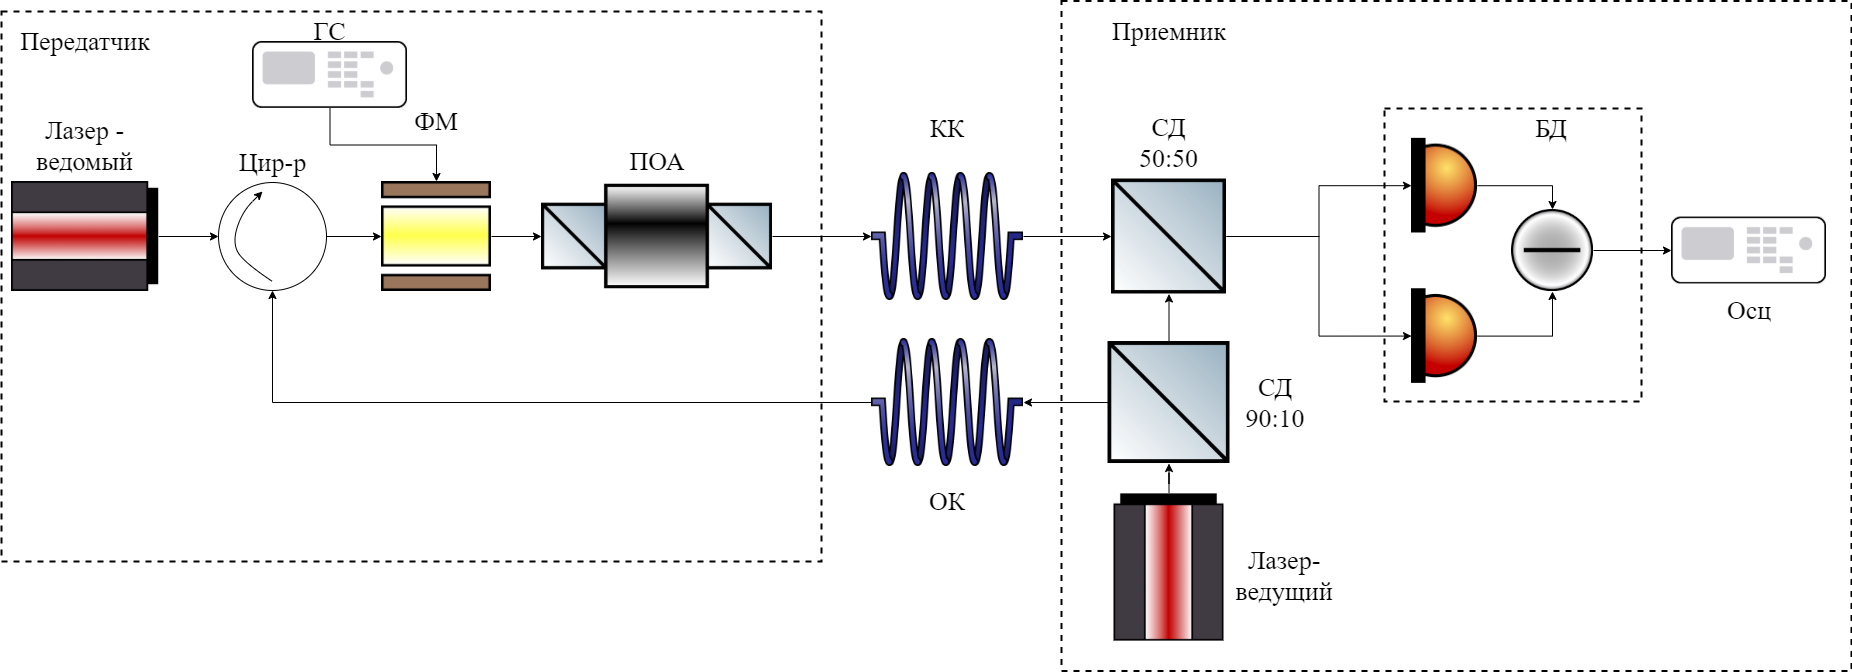
\includegraphics[width=\linewidth]{images/Схема с обратной связью новая 2 .png}
    \caption{Оптическая схема установки системы КРК на поднесущих гармониках с оптической инжекцией, где СД - светоделитель, ГС - генератор сигналов, ФМ - фазовый модулятор, ПОА - переменный оптический аттенюатор, КК - квантовый канал, ОК - открытый канал, Цир-р - циркулятор, БД - балансный детектор, Осц - осциллограф}
    \label{fig:feedback scheme ch2}
\end{figure}
Данная схема работает следующим образом. Лазер-ведущий генерирует оптическое излучение, которое разделяется на 2 части светоделителем 90:10, 10 процентов которого по открытому каналу передаются на сторону передатчика в 1 порт оптического циркулятора. Во второй порт циркулятора подключен лазер передатчика. Такая схема подключения как раз создает оптическую инжекцию и частоты лазера передатчика и лазера локального осциллятора совпадают. Полученное излучение на стороне передатчика проходит фазовую модуляцию с помощью связки фазового модулятора и генератора сигналов произвольной формы на частоте 100 МГц. После этого подготовленный сигнал ослабляется с помощью переменного оптического аттенюатора. После этого излучение передается по квантовому каналу на сторону приемника. В приемнике принятый сигнал попадает на симметричный светоделитель с 2 входами и 2 выходами с коэффициентом деления 50:50. На второй же вход этого делителя попадает излучение ЛО, его 90 процентов после светоделителя. В итоге эти сигналы интерферируют и результат этой интерференции регистрируется балансным детектором. Так как длины волн информационного лазера и ЛО совпадают, то в результате интерференции они регистрируются как постоянный уровень напряжения, однако благодаря выносу фазово-кодированных состояний на поднесущие гармоники, то их интерференция с ЛО и дает результат в виде промежуточной частоты, которая равна частоте модуляции, применённой в Алисе. Эта частота на выходе балансного детектора оцифровывается с помощью осциллографа и в дальнейшем обрабатывается. 
\section{Полученные экспериментальные результаты}\label{sec:ch2/sect6}

В результате интерференции на выходе балансного детектора регистрируется промежуточная частота равная $\omega + \Omega - F$, где $\omega$ - частота лазера Алисы, $\Omega$ - частота модуляции, F - частота ЛО. Благодаря применению оптической инжекции частоты ЛО и лазера Алисы совпадают, поэтому на выходе балансного детектора остается только гармоника на частоте модуляции, в которую и вносится фазовый сдвиг для передачи информации. Этот сигнал изображен на рисунке \ref{fig:100 MHZ filt ch2}
\begin{figure}
    \centering
    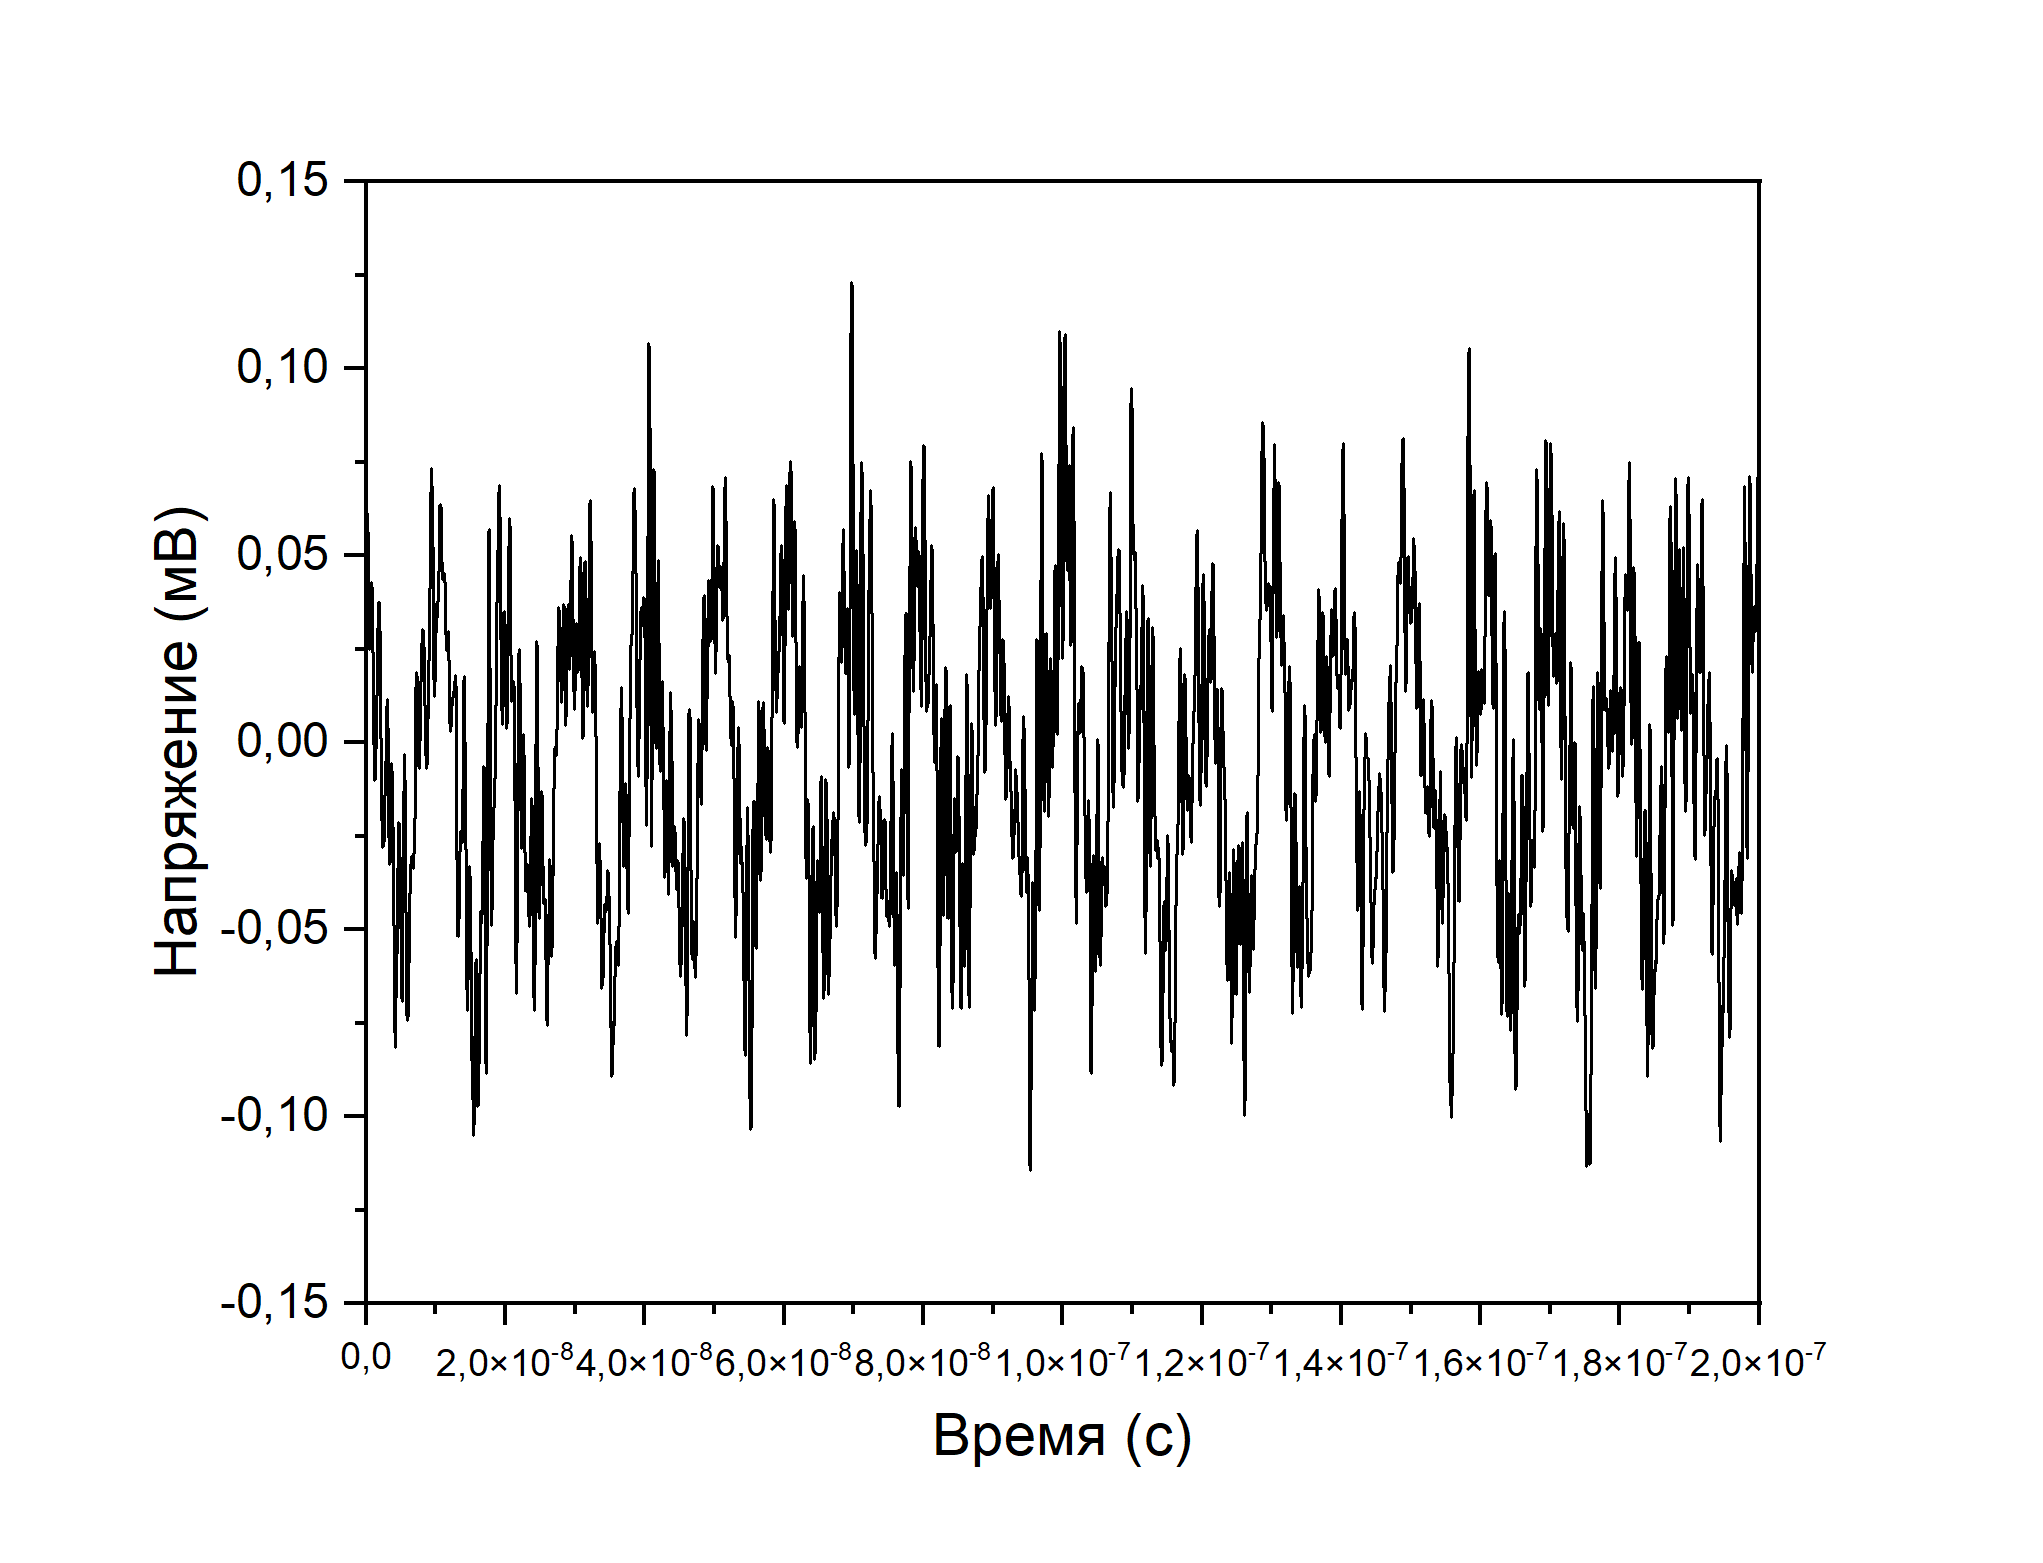
\includegraphics[width=\linewidth]{images/сигнал после бд с новыми шкалами.png}
    \caption{Выходной зашумленный сигнал на выходе балансного детектора.}
    \label{fig:100 MHZ filt ch2}
\end{figure}
На этом графике видна один гармонический сигнал в 100 МГц, в котором содержится информация о фазе, которую необходимо извлечь методами цифровой обработки сигналов. Для более точного измерения фазы сигнала, необходимо эту частоту отфильтровать от шума, который появляется из-за прохождения канала и собственных шумов балансного детектора. Результат цифровой фильтрации сигнала с рисунка \ref{fig:100 MHZ filt ch2} отображается ниже. 
\begin{figure}
    \centering
    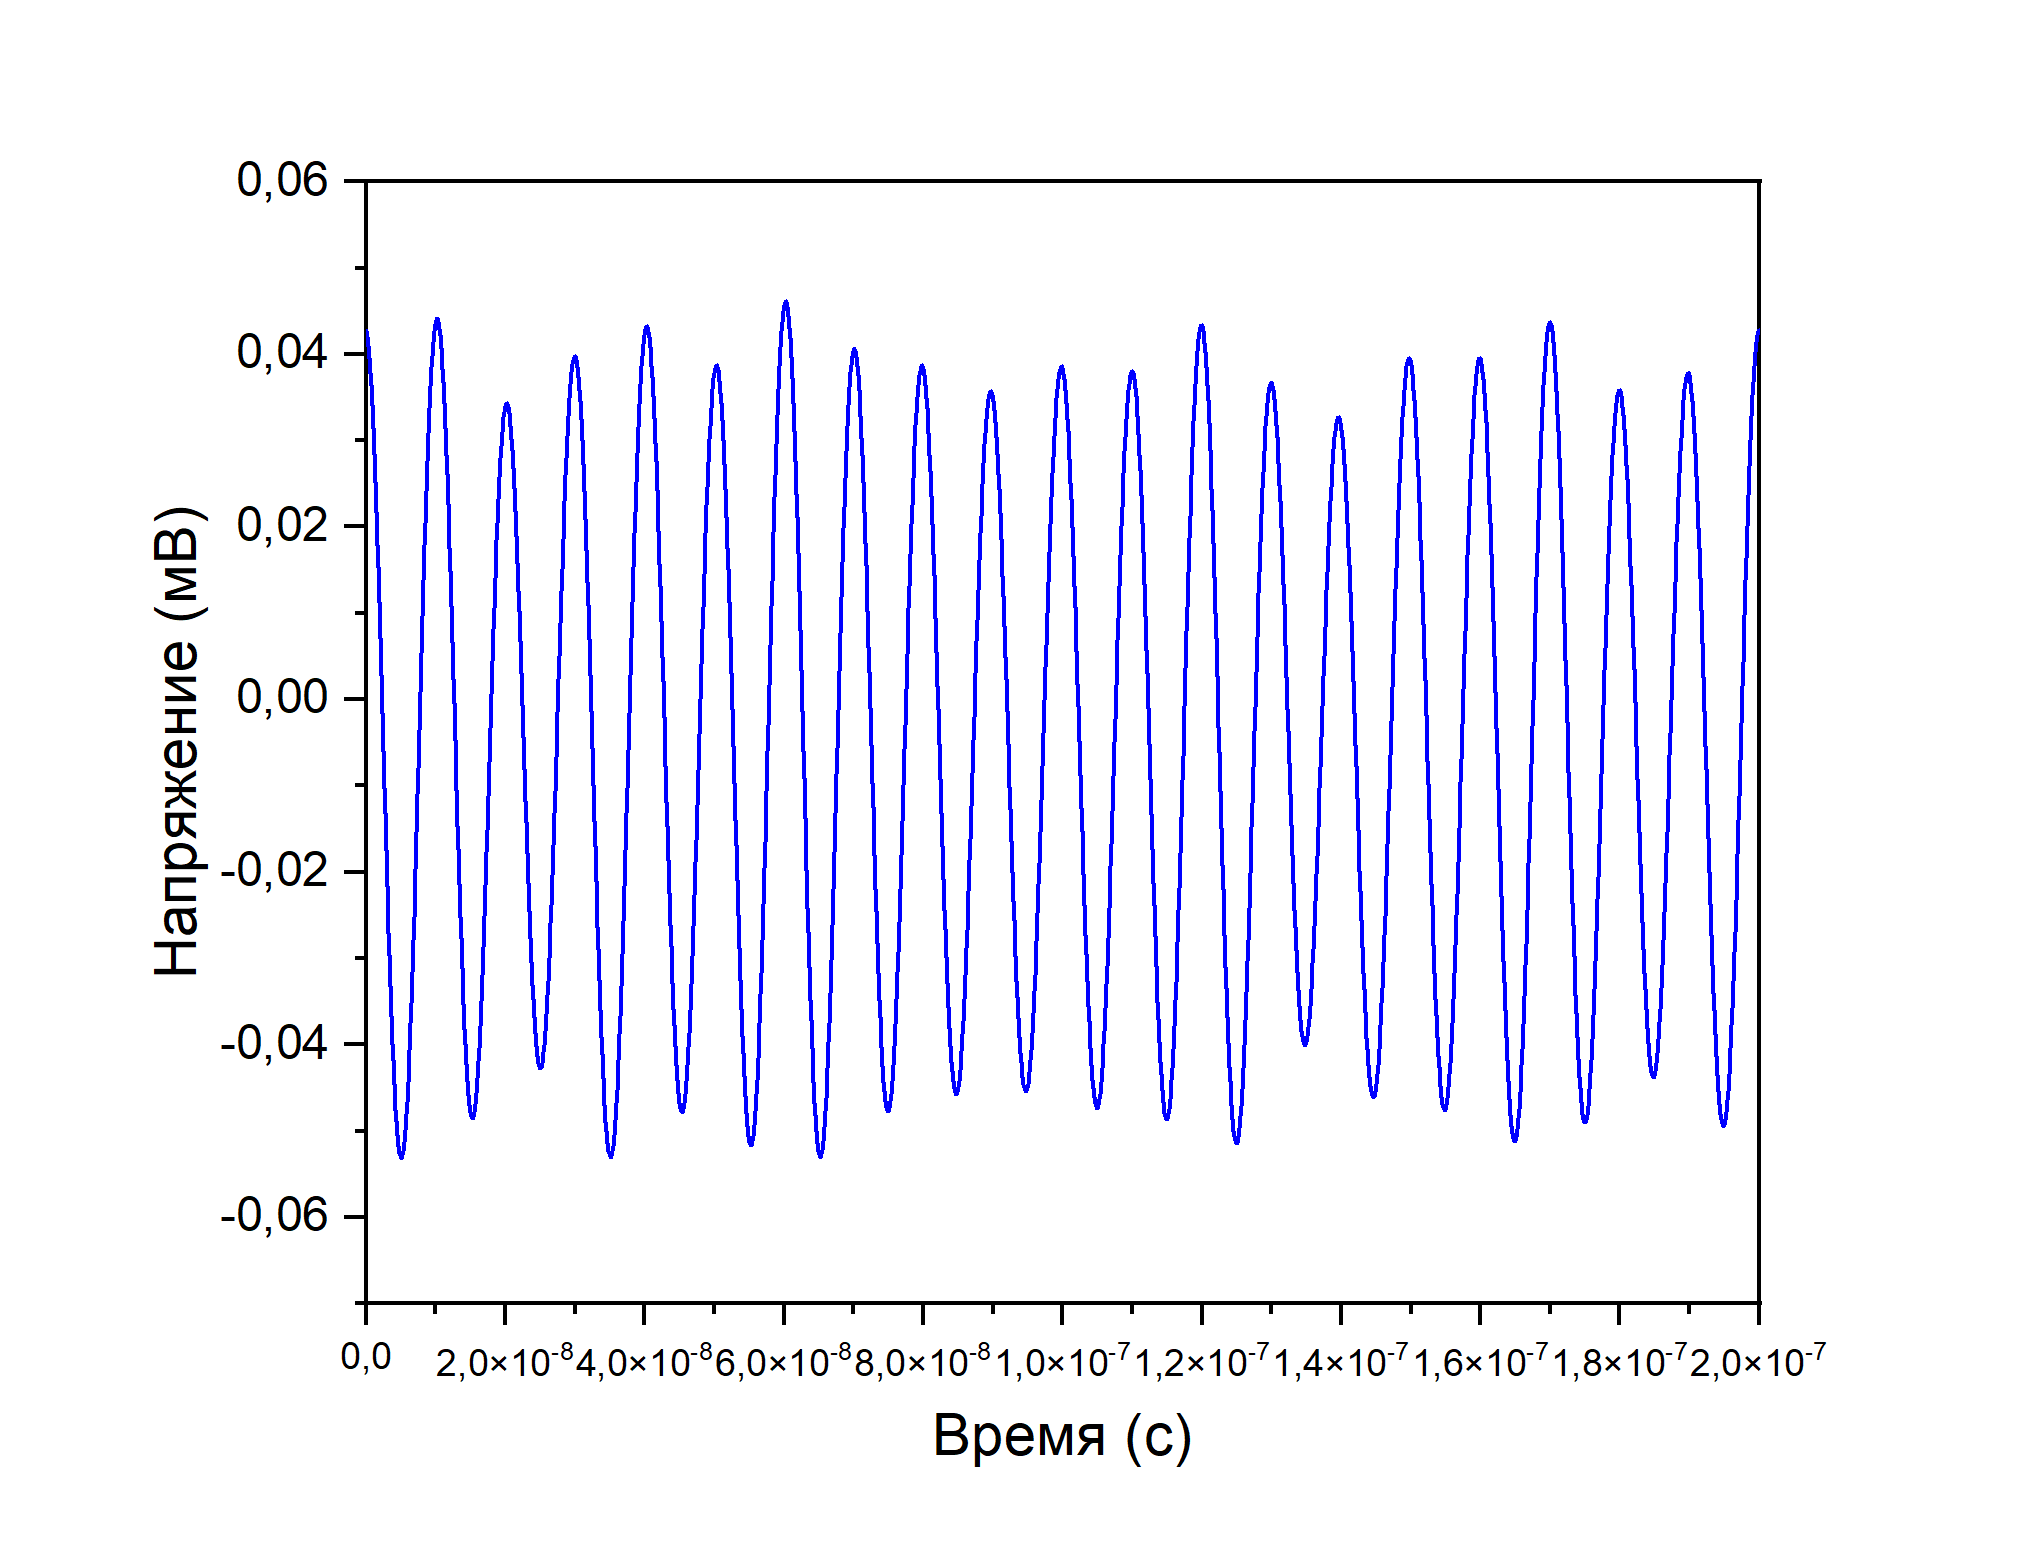
\includegraphics[width=\linewidth]{images/фильтрованное с новыми шкалами.png}
    \caption{Выходной сигнал балансного детектора после фильтрации.}
    \label{fig:filter 100 mhz ch2}
\end{figure}
После применения к сигналу с рисунка \ref{fig:filter 100 mhz ch2} алгоритма Быстрого Преобразования Фурье для изучения спектрального состава. Результат изображен на рисунке ниже.
\begin{figure}
    \centering
    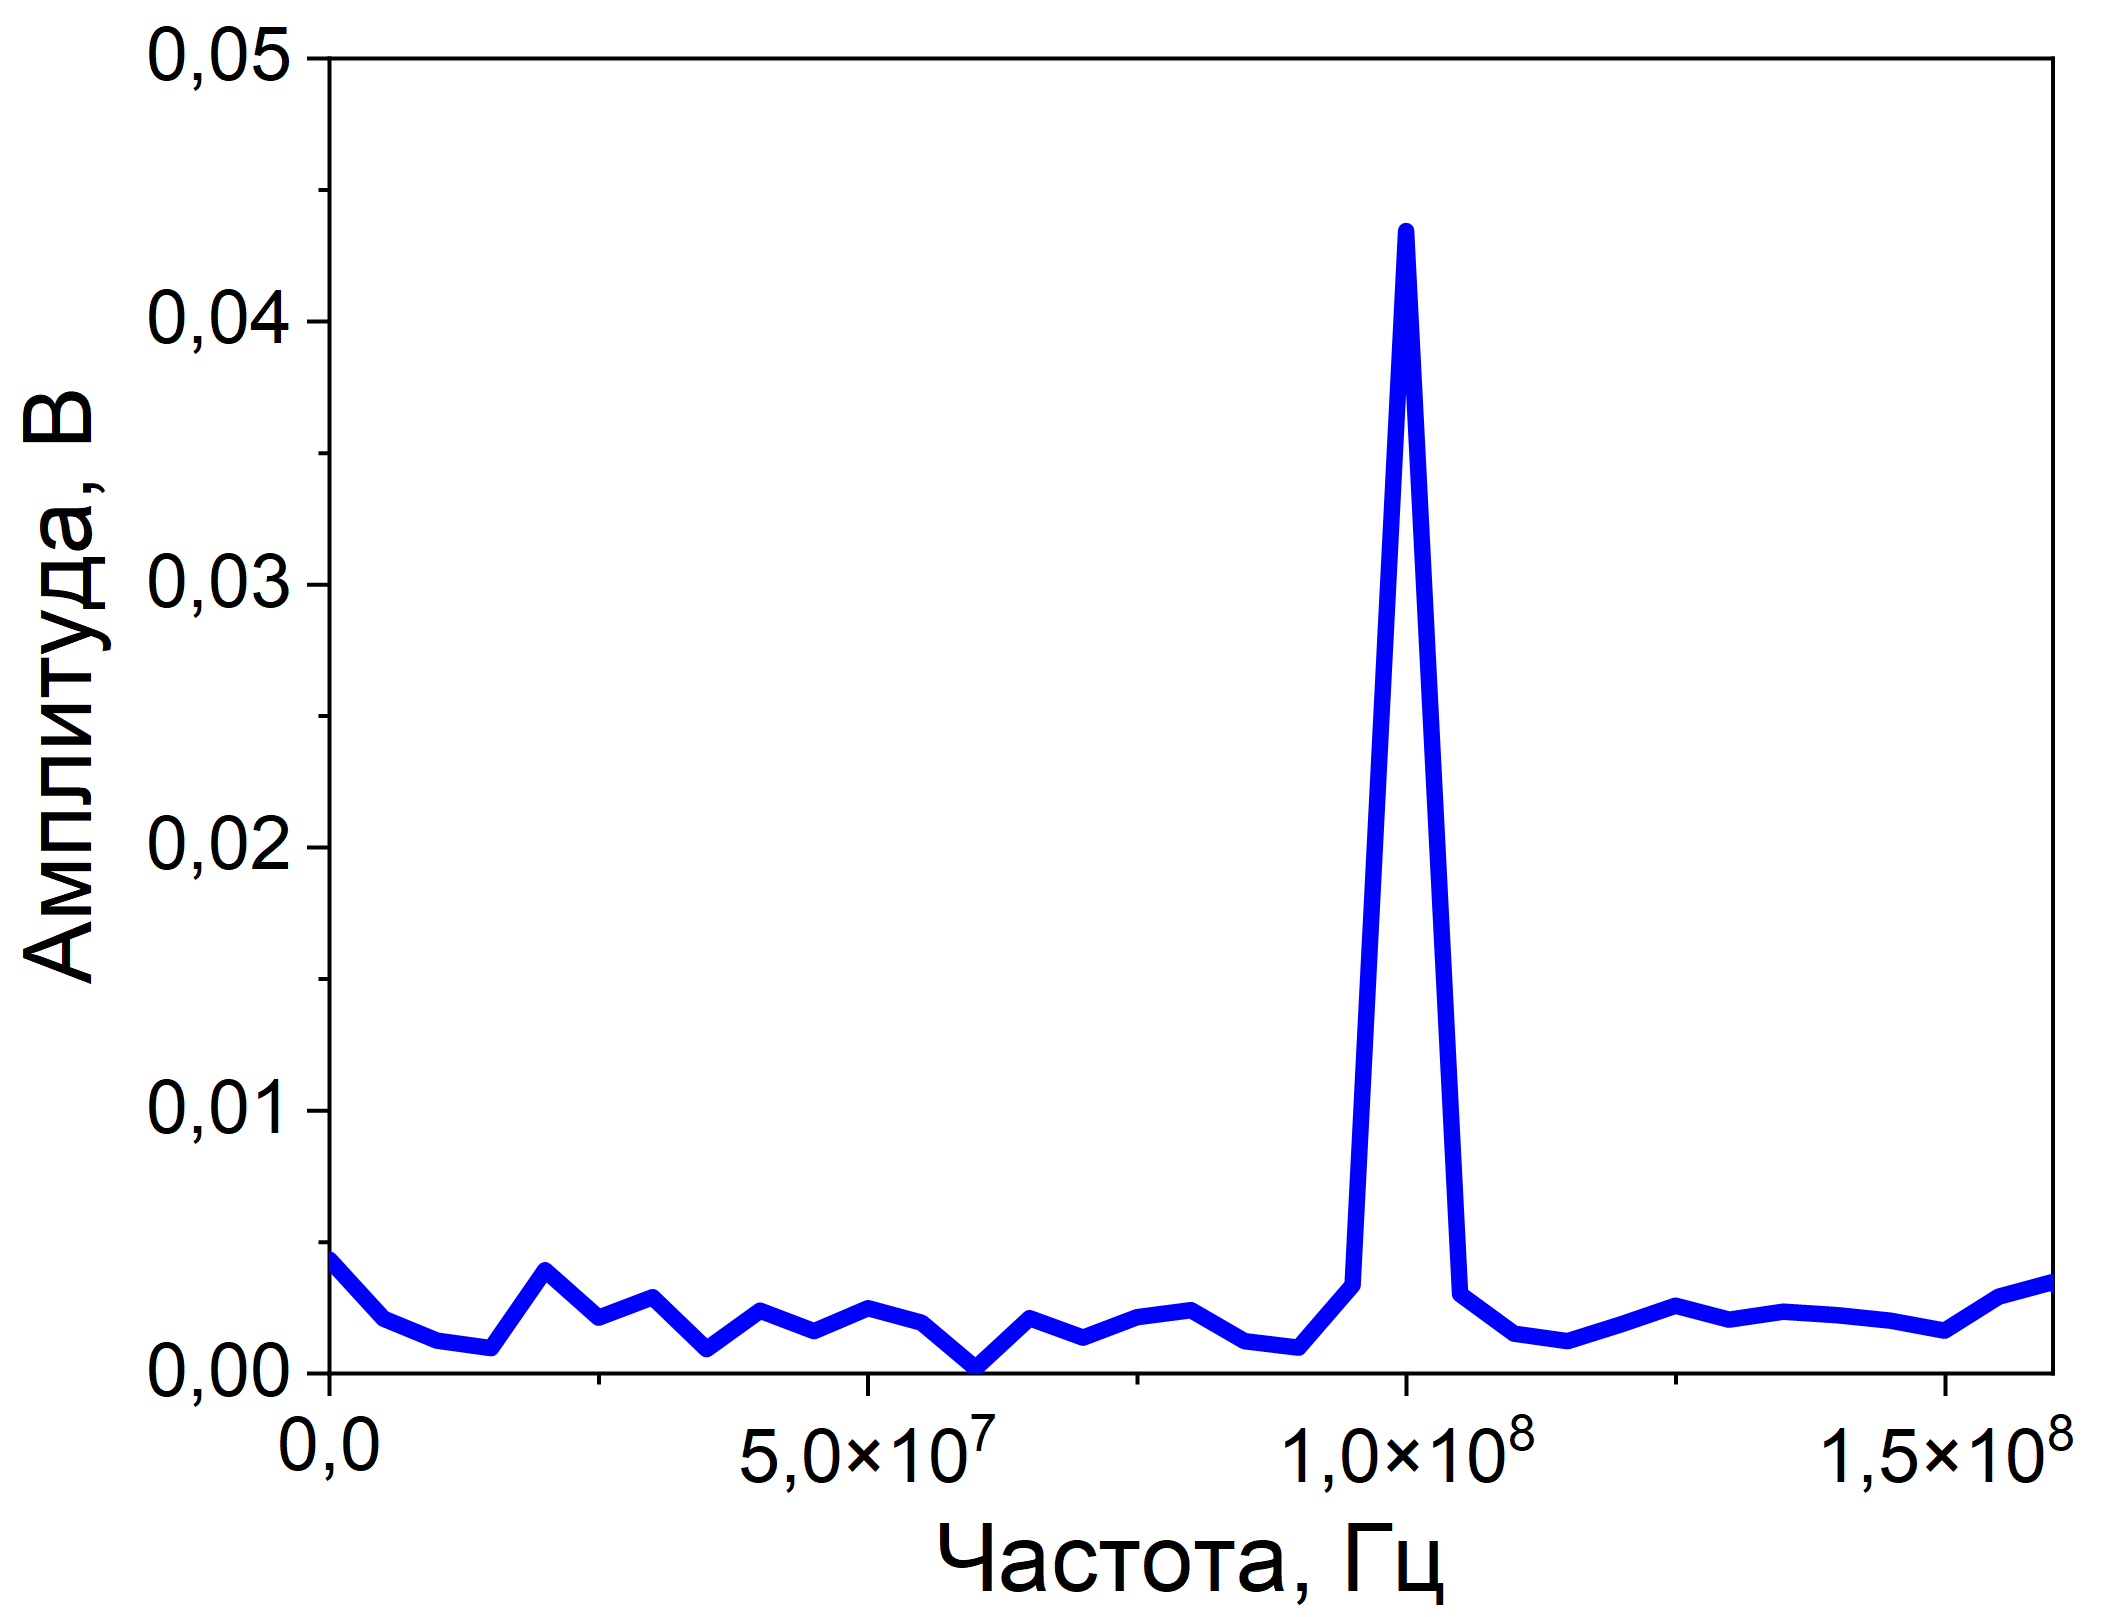
\includegraphics[width=0.7\linewidth]{images/05.png}
    \caption{Спектр полученного сигнала}
    \label{fig:spectrum ch2}
\end{figure}
На рисунке \ref{fig:spectrum ch2} изображен результат БПФ, применённого к сигналу после фильтрации. Единственная гармоника находится на частоте 100 МГц, что согласуется с тем, что частоты лазеров-ведущего и лазера-ведомого совпадают.
Для получения информации о фазе принятого сигнала необходимо цифровыми методами обработки информации извлечь ее оттуда. Для этого также возможно использование быстрого преобразования Фурье. Результат этого преобразования отображен на рисунке \ref{fig:phase meas ch2} 
\begin{figure}
    \centering
    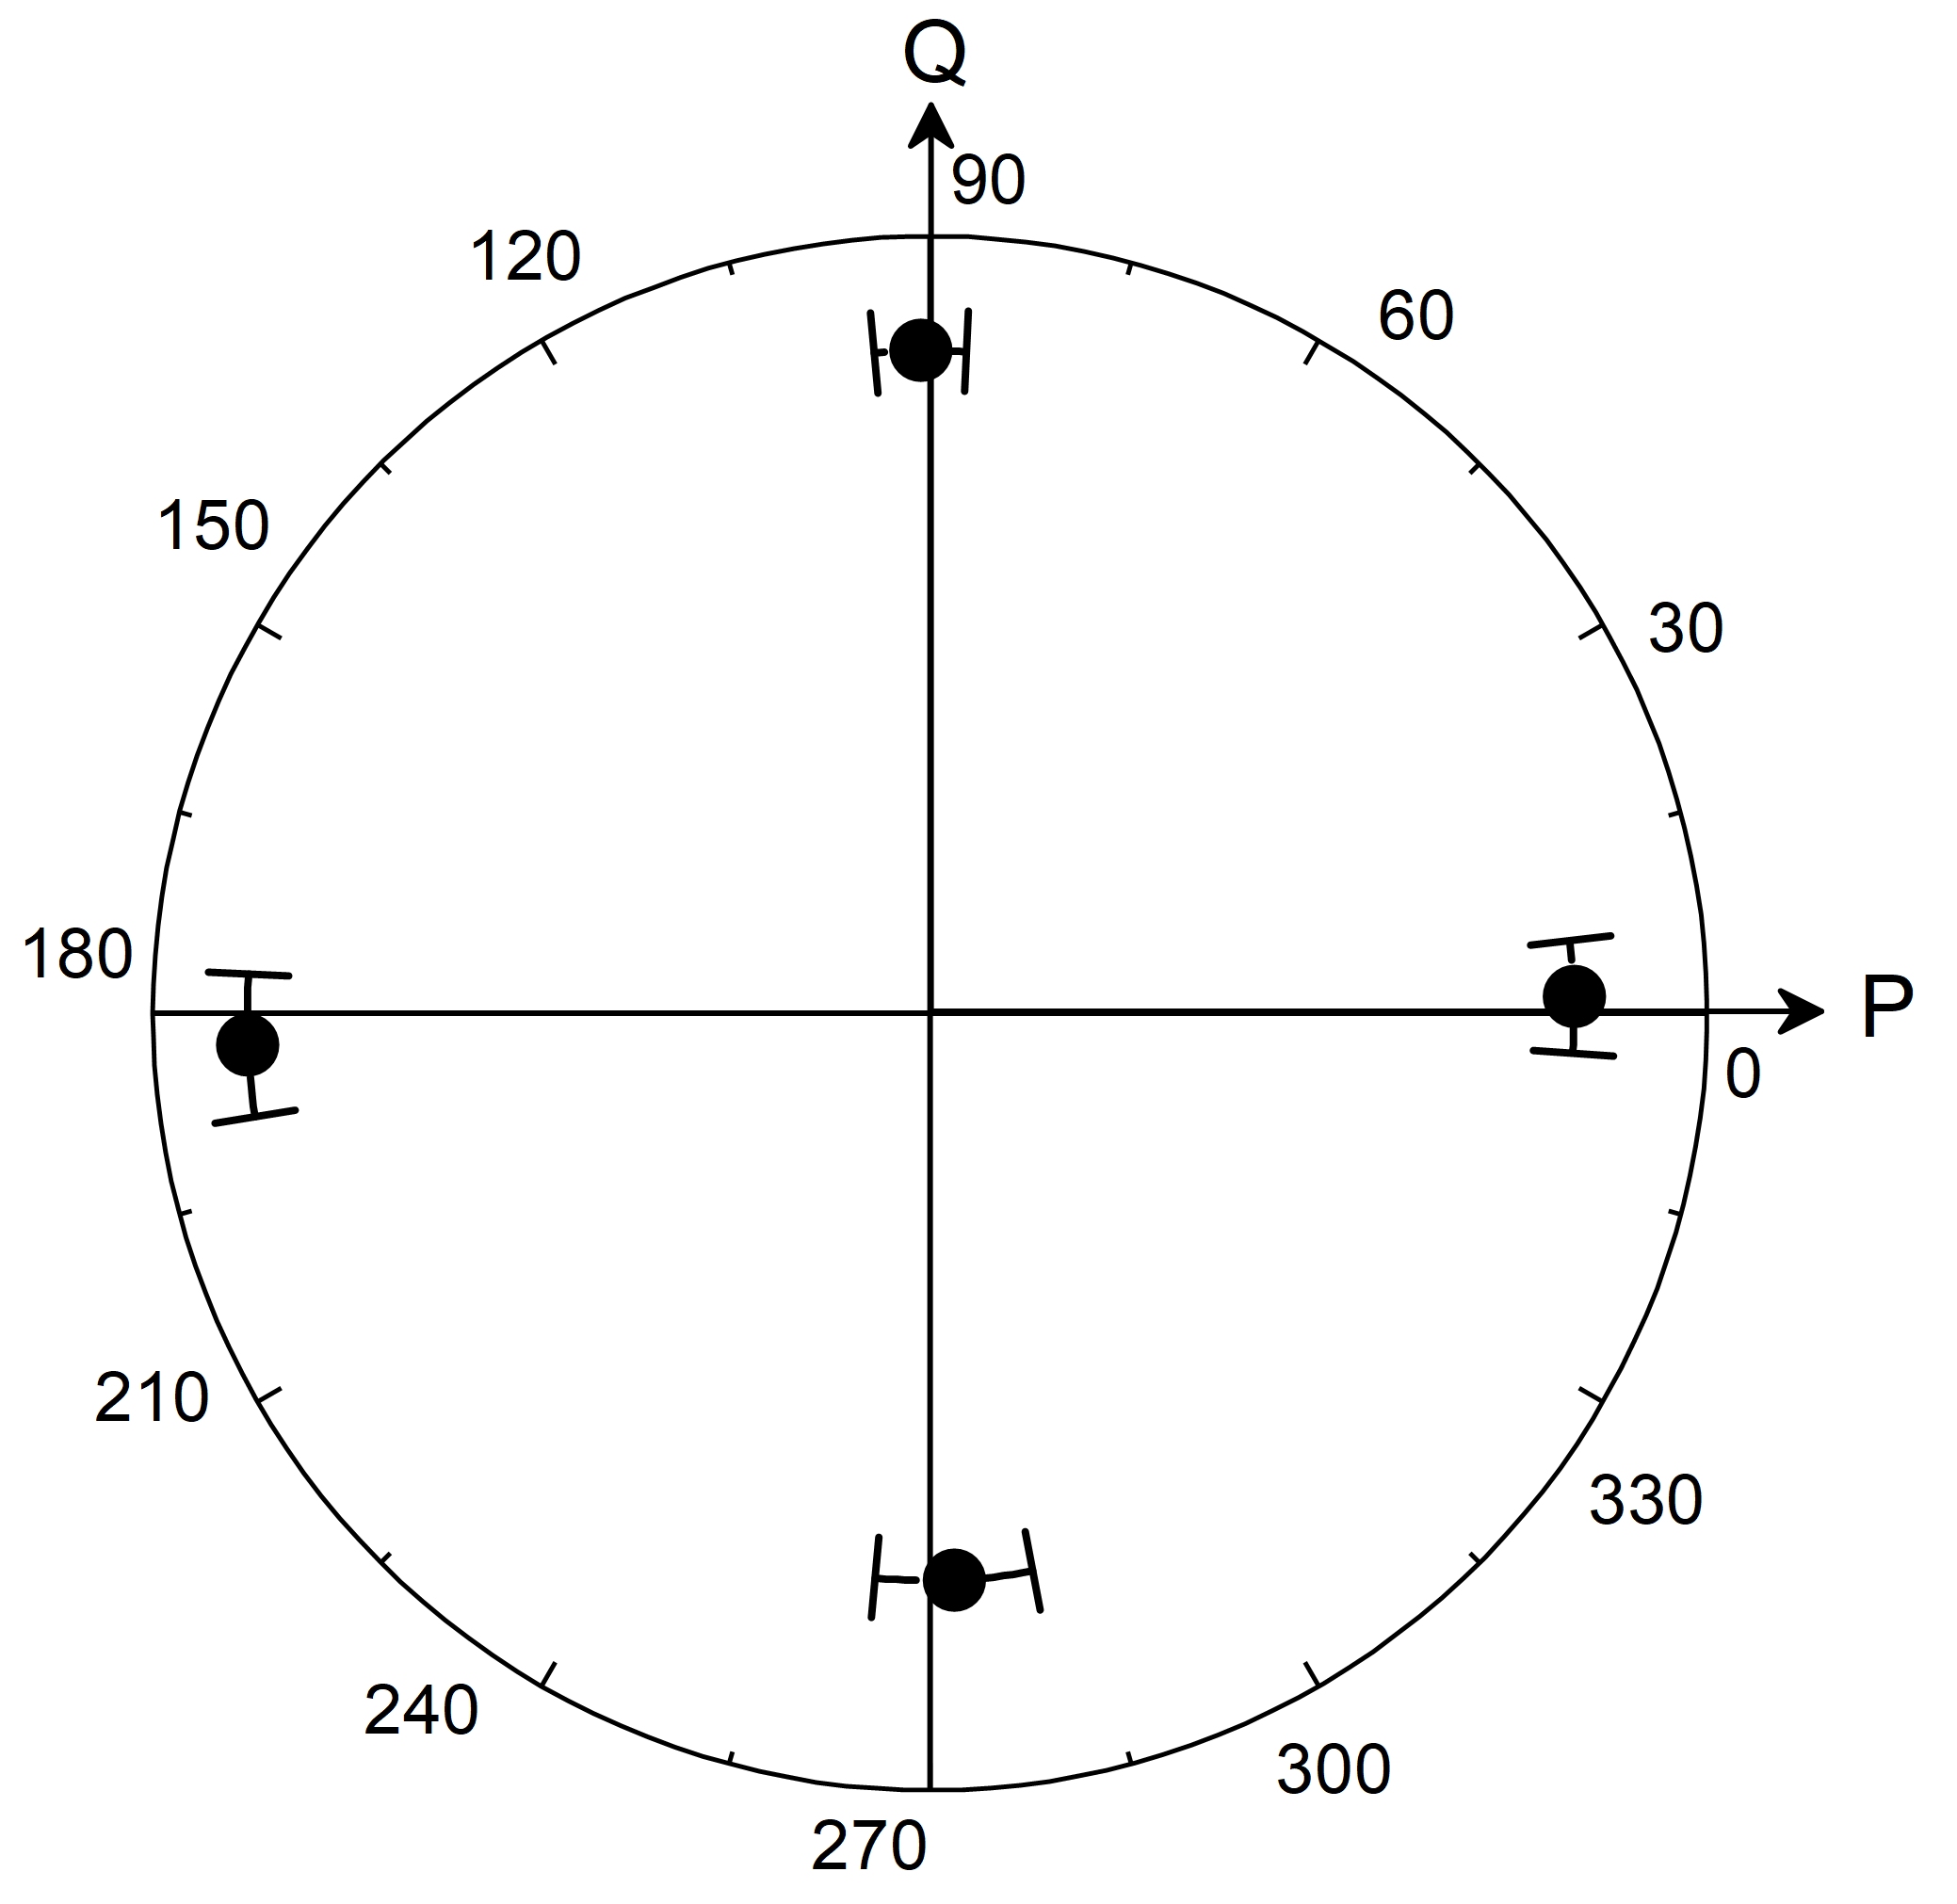
\includegraphics[width=0.6\linewidth]{new_iq_graph_het_true.png}
    \caption{Измеренные значения фазовых сдвигов в выходном сигнале балансного детектора}
    \label{fig:phase meas ch2}
\end{figure}
В результате работы алгоритма по извлечению информации из принятого сигнала, на выходе формируется последовательность фазовых сдвигов, которым сопоставляется определенному значению бита. Такая последовательность будет являться сырым ключом. На рисунке \ref{fig:phase meas ch2} изображены как раз фазовые сдвиги, которые соответствуют виду модуляции QPSK, которые широко распространена в классических системах передачи данных.
Благодаря этому можно передавать 2 бита информации за один такт передачи данных. 

\section{Выводы по главе}\label{sec:ch2/sect8}
В данной главе впервые рассматривается применение обратной связи для системы квантового распределения ключей на боковых частотах на непрерывных переменных в виде оптической инжекции. Такая обратная связь, применяемая к гетеродинному методу детектирования, позволяет стабилизировать частоты лазеров-отправитель и лазер Локального Осциллятора с точностью до нескольких мегагерц.
Такая точность позволяет не выполнять подстройку частоты, как в системах с двумя независимыми источниками излучения. В рамках главы также рассмотрен схема оптического эксперимента по распределению последовательности сырых бит, в рамках которой проведена фильтрация сигнала на промежуточной частоте и его постобработка для извлечения фазы сигнала и, соответственно, бит информации.
Данный метод требует наличия дополнительного оптического канала для создания обратной связи и более тщательного исследования на уязвимость технической реализации для дальнейшего внедрения в реальные системы КРК.
           % Глава 2
\chapter{Система квантового распределения ключа на поднесущих гармониках с применением двух независимых источников когерентного излучения на непрерывных переменных}\label{ch:ch3}
Первые системы квантового распределения ключа на непрерывных переменных основывались на генерации и локального осциллятора, и квантовых состояний, одним лазером \cite{diamanti2015}. Это позволяло избегать проблем с рассогласованием фаз ЛО и квантовых состояний. Однако, это несло и существенные недостатки. Была необходима система мультиплексирования на стороне передатчика и демультиплексирования на стороне приемника для того, чтобы была возможность передавать локальный осциллятор в одном же волокне с квантовыми состояниями без нежелательной интерференции ЛО с ними. Другим недостатком являлась ограниченная мощность передаваемого локального осциллятора. Это связано с несколькими причинами. Первая причина - при передаче по ВОЛС локальный осциллятор затухает, как и все сигналы, проходящие по волокну, что ограничивает его мощность на этапе интерференции в приемном модуле \cite{tang2020}. Вторая причина ограничения мощности локального осциллятора - нелинейные эффекты, возникающие во время прохода мощного сигнала по волоконно-оптическому тракту, связанный с рассеянием Рэлея и прочими. Соответственно, передача мощного ЛО может перекрыть все преимущества его мощности дополнительными шумами. И самая главная проблема - это возможные атаки на ЛО от злоумышленника \cite{jouguet2013}. Итогом всех этих проблем стало использование "локального" локального осциллятора на стороне приемника, сгенерированного отдельным независимым лазером \cite{khaksar2023, adan2024, laudenbach2019a, wang2018b}.
\section{Метод гетеродинного детектирования сигналов для системы квантового распределения ключа на боковых частотах}\label{sec:ch3/sec1} 
В данной главе предлагается использование гетеродинного метода детектирования сигнала с применением двух независимых источников когерентного излучения на непрерывных переменных. Данный способ обладает следующими достоинствами
\begin{enumerate}
    \item Использование источника ЛО на стороне приемника решает проблемы передачи ЛО в канале, связанные с шумом и недостаточной мощностью
    \item Оптическая схема с ЛО на стороне приемника защищает этот источник от атак злоумышленника, что существенно повышает устойчивость данной системы к воздействию злоумышленника
    \item При гетеродинном приеме сигнала, информация о принятом сигнале переносится в полосу радиочастот на промежуточную частоту, что позволяет анализировать и усиливать гармоническое колебание, что существенно расширяет возможность по применяемым видам модуляции
    \item Применение гетеродинного метода детектирования сигналов также позволяет разделять частотно-мультиплексированные сигналы на одну несущую оптическую частоту для повышения скорости выработки секретного ключа или повышения секретности за счет случайного выбора рабочей частоты.
\end{enumerate}
Современные работы по созданию систем КРК на непрерывных переменных переходят к использованию ЛО, сгенерированного на стороне приемника. В данной работе рассматривается применение двух независимых источников излучения для системы квантового распределения ключа на поднесущих гармониках и с частотным мультиплексированнием на одной несущей частоте.
\section{Протокол квантового распределения ключа на поднесущих гармониках с гетеродинном методом детектирования сигналов}\label{sec:ch3/sect2}
Протокол работает следующим образом:
\begin{enumerate}
    \item Алиса готовит квантовые состояния, кодируя информацию в фазовый сдвиг излучения на боковых частотах ослабленного лазерного излучения, и передает их.
    \item Боб измеряет пришедшие квантовые состояния с помощью гетеродинного детектирования.
    \item Выходной сигнал балансного детектора оцифровывается и обрабатывается с помощью алгоритма Быстрого Преобразования Фурье.
    \item Измеряется частота и фаза нужной гармоники из полученного мгновенного спектра.
    \item Оценивается соотношение сигнал/шум.
    \item Проводится процедура исправления ошибок с помощью соответствующих кодов.
\end{enumerate}
\section{Оптическая схема системы квантового распределения ключа на боковых частотах с применением гетеродинного детектирования }\label{sec:ch3/sect5}
Данная схема устроена следующим образом. Лазер на стороне передатчика генерирует непрерывное лазерное излучение. Это излучение проходит по оптическому волокну с сохранением поляризации и попадает на фазовый модулятор. На фазовый модулятор попадает сигнал от генератора сигналов свободной формы. Этот генератор подготавливает модулирующий сигнал. В нем содержаться фазовые сдвиги, которые соответствуют кодировке QPSK с фазами 45, 135, 215 и 305 градусов \cite{karinou2018}. Этот сигнал модулирует оптическое излучение и на выходе получаются дополнительные поднесущие гармоники сигнала в выходном спектре фазового модулятора. После этого сигнал попадает на волоконно-оптический перестраиваемый аттенюатор для снижения уровня мощности на поднесущих гармониках до однофотонного уровня \cite{oxborrow2005}.
После этого сигнал проходит квантовый канал и попадает на схему контроля поляризации, которая рассматривается в секции \ref{sec:ch3/sect4}. После прохождения этой схемы, сигнал попадает на светоделитель с 2 входами и 2 выходами с коэффициентом деления 50:50, на входы которого попадает и сигнал локального осциллятора. В результате происходит интерференция этих сигналов. Но частоты ЛО и информационного сигнала отличаются так, что частота ЛО больше частоты лазера передатчика. В итоге этот результат интерференции регистрируется балансным детектором. Разностные частоты от всех сигналов, которые проинтерферировали, находятся в полосе пропускания балансного детектора благодаря подбору частот. При необходимости частота лазера ЛО может быть подстроена для переноса спектра сигнала вверх или вниз по частоте. По итогу на выходе БД формируется несколько гармонических колебаний. Для анализа необходимо отфильтровать синусоидальное колебание на частоте модуляции, так как оно несет информацию о фазе, закодированной передатчиком. После этого его можно обрабатывать уже методами цифровой обработки сигналов (ЦОС). Для компенсации же фазовых искажений можно обрабатывать промежуточную частоту между лазерами передатчика и приемника. Ее фазовые колебания будут содержать фазовый шум и передатчика с квантовым каналом, и фазовый шум ЛО. Это измеренное значение необходимо учитывать на этапе постобработки. 
Оптическая схема гетеродинного метода детектирования для системы КРК приведена на рисунке \ref*{fig:het true ch3} 
\begin{figure}
    \centering
    \includegraphics[width = \linewidth]{images/Гетеродин схема новая2 .png}
    \caption{Схема эксперимента по реализации гетеродинного метода приема сигналов для КРК, где ГС - генератор сигналов, ФМ - фазовый модулятор, ПОА - перестраиваемый оптический аттенюатор, КК - квантовый канал, КП - контроллер поляризации, СД - светоделитель, ФД - фотодиод, ЛО - локальный осциллятор, БД - балансный детектор, ОСЦ - осциллограф}
    \label{fig:het true ch3}
\end{figure}
\section{Математическая модель системы квантового распределения ключа на боковых частотах с применением гетеродинного детектирования}\label{sec:ch3/sect3}
Излучение лазера может быть представлено следующим образом:
\begin{align}
F(t) = A_0 * \sin(\omega_0 t + \phi_0),
\end{align}
где $A_0$ -- амплитуда сигнала, $\omega_0$ -- частота лазерного излучения, $\phi_0$ -- начальная фаза излучения.
Модулирующий сигнал:
\begin{align}
S(t) = (1+ m\sin(\Omega t  + \phi (t))),
\end{align} 
где $m$ -- индекс модуляции, $\Omega$ -- частота модуляции, $\phi (t)$ -- вносимая модуляция.

Лазерное излучение после модуляции выглядит следующим образом:
\begin{align}
\label{eq:laser_het}
F_s(t) &= F(t) * S(t) = A_0 * \sin(\omega_0 t + \phi_0) + \frac{A_0 * m}{2} * (\cos((\omega_0 + \Omega)t + (\phi_0 + \phi (t))) - \notag \\
&- \frac{A_0 * m}{2} * (\cos((\omega_0 - \Omega)t + (\phi_0 - \phi (t))),
\end{align}

Результат квадратичного детектирования сигнала, полученного в выражении~\eqref{eq:laser} будет выглядеть следующим образом:
\begin{equation}
    \begin{aligned}
        &F_d(t) = (F(t) * S(t) * F_{het}(t))^2 =
        &\frac{A_{sig}^2*A_{het}^2}{4} + \frac{A_{sig}^2*A_{het}^2 * m^2}{8}
        +\frac{A_{sig}^2*A_{het}^2}{4}*\cos(2ft +2\phi)+\frac{A_{sig}^2*A_{het}^2 *m^2}{8}*\cos(2ft+2\phi)+ \\ 
        &+\frac{A_{sig}^2 *A_{het}^2}{8} * \cos(2ft - 2\omega t) +\frac{A_{sig}^2 *A_{het}^2}{16} * \cos(2ft - 2\omega t)+\\ 
        &+\frac{A_{sig}^2*A_{het}^2}{4}*\cos(2\omega*t +2\phi) +\frac{A_{sig}^2*A_{het}^2 *m^2}{8}*\cos(2\omega*t +2\phi)+  \\&
        +\frac{A_{sig}^2*A_{het}^2}{8} + \cos(2ft + 2\omega t + 2\phi) 
        + \frac{A_{sig}^2 * A_{het}^2 * m^2}{16} * \cos(2ft + 2\omega t +4\phi) -   \\& - \frac{A_{sig}^2 * A_{het}^2 * m ^2}{8} * \cos(2\Omega t) - \frac{A_{sig}^2 * A_{het}^2 * m^2}{16} * \cos(2ft - 2\Omega t + 2\phi) -  \\& - \frac{A_{sig}^2 * A_{het}^2 * m^2}{32} * \cos(2ft - 2\omega t - 2\Omega t) - \frac{A_{sig}^2 * A_{het}^2 * m^2}{16}* \cos(2\omega t - 2\Omega t) - \\& - \frac{A_{sig}^2 * A_{het}^2 * m^2}{32}* \cos(2ft + 2\omega t - 2\Omega t + 4\phi) -   \\& - \frac{A_{sig}^2 * A_{het}^2 * m^2}{16} * \cos(2ft + 2\Omega t +2\phi) - \frac{A_{sig}^2 * A_{het}^2 * m^2}{32} * \cos(2ft - 2\omega t + 2\Omega t) -   \\& - \frac{A_{sig}^2 * A_{het}^2 * m^2}{16} * \cos(2\omega t + 2\Omega t + 2\phi) -,
        \frac{A_{sig}^2 * A_{het}^2 * m^2}{32} * \cos(2ft - 2\omega t + 2\Omega t) -   \\& - \frac{A_{sig}^2 * A_{het}^2 * m^2}{16} * \cos(2\omega t + 2\Omega t + 2\phi) - \frac{A_{sig}^2 * A_{het}^2 * m^2}{32} * \cos(2ft + 2\omega t + 2\Omega t + 4\phi)   +   \\& + \frac{A_{sig}^2 * A_{het}^2 * m}{2}* \sin(\Omega t) - \frac{A_{sig}^2 * A_{het}^2 * m}{4} * \sin(2ft - \omega t + 2\phi) - \\& - \frac{A_{sig}^2 * A_{het}^2 * m}{8} * \sin(2ft - 2\omega t - \Omega t) - \frac{A_{sig}^2 * A_{het}^2 * m}{4}* \sin(2\omega t - \Omega t + 2\phi) - \\& - \frac{A_{sig}^2 * A_{het}^2 * m}{8} * \sin(2ft + 2\omega t - \Omega t + 4\phi) + \frac{A_{sig}^2 * A_{het}^2 * m}{2ft + \Omega t + 2\phi} + \\&  +\frac{A_{sig}^2 * A_{het}^2 * m}{8} * \sin(2ft - 2\omega t + \Omega t) + \frac{A_{sig}^2 * A_{het}^2 * m}{4} * \sin(2\omega t + \Omega t + 2\phi) + \\& + \frac{A_{sig}^2 * A_{het}^2 * m}{8} * sin(2ft + 2\omega t + \Omega t + 4\phi)
        \end{aligned}
    \end{equation}\label{eq:het_math_true}
В результате ток, протекающий через фотодиод, будет определяться выражением:
\begin{align}
   I &= R(\lambda)G C F_d,
\end{align} 
где $R(\lambda)$ -- спектральная чувствительность фотодиода, $G$ -- электрическое усиление балансного детектора, $C$ -- отношение апертуры волокна к размеру чувствительной площадки фотодетектора. 

В случае проводимого эксперимента единственная гармоника, которая лежит в полосе пропускания балансного детектора -- это $\frac{A_{sig}^2 *A_{het}^2 *m}{2} * sin(\Omega t)$.
Остальные же гармоники не попадают в полосу пропускания и будут проявляться в виде постоянной составляющей, которая отфильтровывается перед первым усилителем. 

\section{Алгоритм подстройки поляризационных искажений для системы квантового распределения ключа на боковых частотах с применением гетеродинного детектирования}\label{sec:ch3/sect4}
Существенной проблемой для интерференции сигналов является их поляризация \cite{liu2020a}. Как известно, сигналы в ортогональный поляризациях не взаимодействуют. Что существенно снижает эффективность передачи данных в системах КРК на непрерывных переменных. В рамках данного раздела предлагается реализация алгоритма подстройки поляризации пришедшего сигнала.
При использовании связки поляризационного светоделителя и контроллера поляризации можно подстраивать поляризацию за счет анализа спектрального состава принятого сигнала с помощью быстрого преобразования Фурье. В случае неправильной поляризации, на выходе поляризационного светоделителя сигнал разделяется на две поляризации по осям: быструю и медленную. В итоге получается так, что на балансный детектор приходят два сигнала, а не один. Это приводит к тому, что в спектре полученного сигнала появляется не только гармоника на частоте модуляции, но и ее удвоение. Что можно отслеживать и использовать контроллер поляризации для контроля входной поляризации. На рисунке \ref{fig:ruin pol}
\begin{figure}
    \centering
    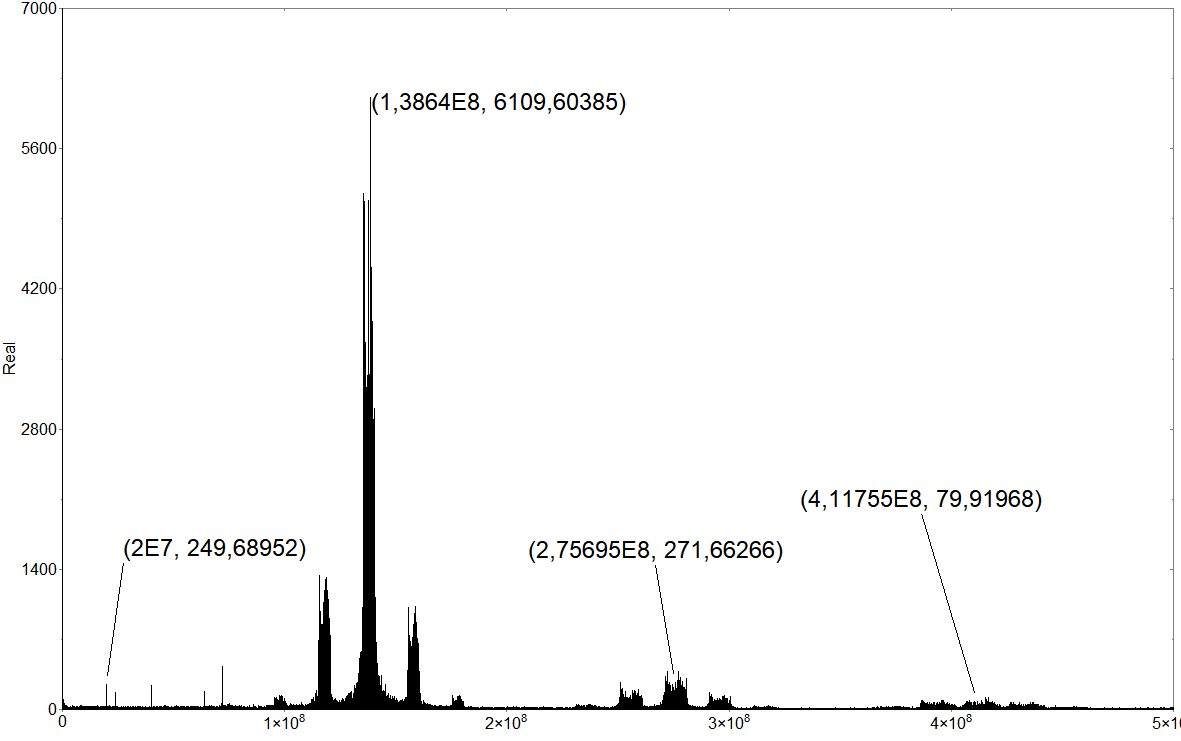
\includegraphics[width = \linewidth]{images/Spectrum of ruined polarization.png}
    \caption{Спектр выходного сигнала с неправильной поляризацией }
    \label{fig:ruin pol}
\end{figure}
В спектре этого сигнала наблюдается гармоники на частоте 20 МГц, что соответствует частоте модулирующего излучения и 40 МГц, что является удвоенной частотой модуляции. На основе этой информации система обратной связи должна дать команду на контроллер поляризации для ее контроля. В результате действий КП должен привести сигнал к виду, отображенному на рисунке \ref{fig:norm pol}
\begin{figure}
    \centering
    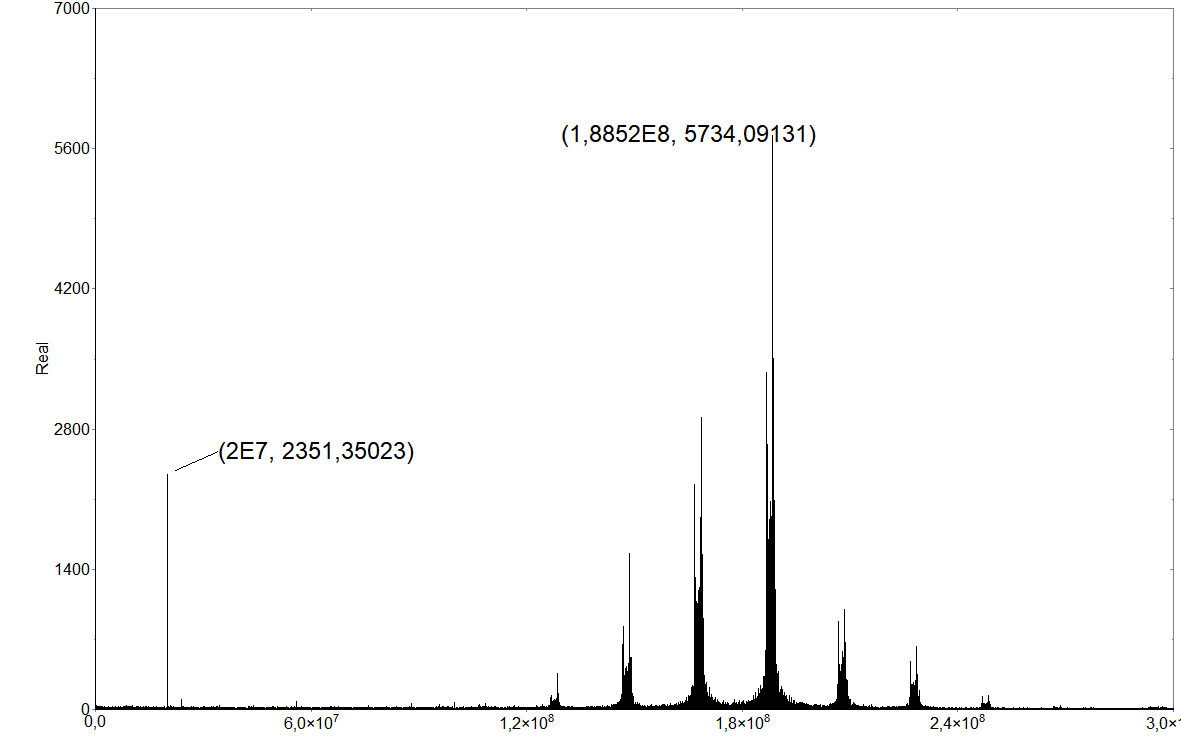
\includegraphics[width = \linewidth]{images/normal polarization.png}
    \caption{Спектр выходного сигнала с балансного детектора с правильной поляризацией}
    \label{fig:norm pol}
\end{figure}
На графике \ref{fig:norm pol} видно, что присутствует только спектральная линия от частоты модуляции и по амплитуде она существенно больше, чем на графике \ref{fig:ruin pol}. 
В общем виде алгоритм можно записать следующим образом
\begin{enumerate}
    \item Применение БПФ к принятому сигналу
    \item Анализ спектрального состава сигнала
    \item Поворот поляризации сигнала до уничтожения гармоники на удвоенной частоте модуляции
    \item Дальнейший поворот поляризации сигнала до максимума гармоники на частоте модуляции
\end{enumerate}
\section{Математическая модель гетеродинного детектирования с двумя независимыми источниками излучения}\label{sec:ch3/sect6}
\section{Описание экспериментальной установки}\label{sec:ch3/sect7}
Для реализации системы квантового распределения ключей на поднесущих гармониках с применением двух независимых источников излучения на непрерывных переменных была собрана экспериментальная схема изображенная на рисунке \ref*{fig:het true ch3}
Данная схема работает следующим образом. Лазерное излучение, сгенерированное лазером NeoPhotonics $\mu$ITLa с шириной линии менее 100 кГц и выходной мощностью 1 мВт и длиной волны 1550.0026 нм. В качестве лазера локального осциллятора использовался лазер Hewlett and Packard 8168C с излучением на длине волны 1550.0018 нм и выходной мощностью 1 мВт. В качестве фазового модулятора использовался фазовый модулятор производства EOSpace с полосой пропускания 40 ГГц и вносимыми потерями 4 дБ.
В качестве балансного детектора использовался детектор фирмы General Photonics BDP-003 с чувствительностью 0.8 А/Вт на длине волны 1550 нм, полосой пропускания 200 МГц и коэффициентом усиления ${10^5}$.
Для измерений и выполнения Быстрого Преобразования Фурье использовался осциллограф Rohde and Schwarz RTM 3000 с полосой пропускания 1 ГГц и количеством выбором 5 ГВ/с.
На электрический же вход фазового модулятора подается гармонический синусоидальный сигнал с частотой 20 МГц и амплитудой 1 В и дополнительным смещением в 0.8 В. В результате взаимодействия лазерного излучения и электрического сигнала на фазовом модуляторе в спектре излучения образуются 2 дополнительные гармоники - боковые частоты.
Полученный сигнал попадает на переменный оптический аттенюатор, который вносит затухание таким образом, чтобы на боковых частотах был уровень сигнала, мощность которого в среднем меньше мощности одного фотона.
После этого полученный сигнал передается по одномодовому оптическому волокну на сторону приемника. Попав на сторону приемника, сигнал попадает на блок контроля поляризации, о принципе работы которого будет рассказано позже. Прошедший сигнал попадает на один из входов светоделителя с 2 входами и 2 выходами и коэффициентом деления 50:50.
На другой же вход светоделителя попадает излучение лазера - локального осциллятора (ЛО). В результате на светоделителе квантовые состояния от Алисы интерферируют с локальным осциллятором. За счет этой интерференции с мощным ЛО, квантовые состояния усиливаются и регистрируются балансным детектором, который основан на двух классических фотодиодах.

\section{Описание полученных результатов}\label{sec:ch3/sect8}
При интерференции локального осциллятора и квантовых состояний, посланных Алисой, на светоделителе на стороне Боба, формируются комбинационные частоты от всех спектральных составляющих. Их модели описаны в разделе \ref*{sec:ch3/sect6}.
В полученной модели интерес представляют только разностные частоты по причине того, что только они попадают в полосу пропускания балансного детектора.
На выходе балансного детектора формируется гармонический сигнал состоящий из двух огибающих и несущей. Форма этого сигнала изображена на рисунке \ref*{fig: het true time}
\begin{figure}
    \centering
    \includegraphics*{толстые линии и исправлены названия сигнал после детектирования.png}
    \caption*{Выходной сигнал с балансного детектора во временной области}
    \label{fig: het true time}
\end{figure}
Информацию несут только огибающие данного сигнала. Для их анализа их предварительно необходимо отфильтровать. Это можно сделать как программными методами, так и с помощью физических фильтров, установленных после балансного детектора.
В рамках данной работы предлагается программно фильтровать огибающую, которая соответствует частоте $(\omega_{LO} -(\omega_{car} - \Omega_{mod})$, так как она попадает в полосу пропускания балансного детектора. 

В результате работы данной системы на выходе балансного детектора формируются сигналы на промежуточных частотах, которые соответствуют разности частот локального осциллятора и частот сигналов, пришедших от Алисы. Спектр сигнала изображен на рисунке \ref*{label}

\section{Выводы по главе}\label{sec:ch3/sect9}
В данной главе впервые изучено применение двух независимых источников излучения для передачи квантовых состояний света в системе квантового распределения ключей на непрерывных переменных на боковых частотах. Данный подход позволяет распределять сырую последовательность бит в системе КРКБЧ-НП с гетеродинным методом детектирования. 
Благодаря которому информация об измеренных квантовых состояниях переносится на промежуточную частоту, которая лежит в полосе балансного детектора, что значительно упрощает фильтрацию и усиление, так как эта частота находится в радиодиапазоне, где эти операции известны и отработаны. Другим преимуществом является то, что благодаря переносу на промежуточную частоту возможно применять любой вид модуляции будь то фазовая или амплитудно-фазовая без дополнительных элементов, что существенно улучшает гибкость и характеристики системы относительно гомодинного метода детектирования.
Также в этой главе решается проблема контроля поляризации в системах с двумя независимыми источниками излучения и гетеродинным методом детектирования. Данный метод основывается на Быстром Преобразовании Фурье и использовании активного контроллера поляризации для быстрой ее подстройки, что позволит контролировать поляризацию на лету, не ограничивая скорость выработки сырой последовательности.           % Глава 3
\chapter{Атака оптической накачкой на источник когерентного излучения}\label{ch:ch4}
\renewcommand{\thefigure}{4.\arabic{figure}} % Plain numbering
\setcounter{figure}{0}                     % Reset if needed
\renewcommand{\thetable}{4.\arabic{table}}



Использование технологии квантового распределения ключей дает абсолютную защиту информации от доступа злоумышленника за счет использования метода одноразовых блокнотов для шифрования данных и за счет использования одиночных фотонов в качестве носителей ключа для его передачи через оптические линии связи, применение которых обеспечивает безопасность за счет фундаментальных законов квантовой физики \cite{bennett1984,horodecki2008}. Однако несовершенство технических компонентов, применяемых в практических реализациях систем КРК, может дать злоумышленнику доступ к секретному ключу за счет внесения изменений в функционирование элементов или, что хуже, полностью контролировать их работу \cite{lo2014,dixon2017,xu2020,makarov2023}. Поэтому критически необходимо исследовать потенциальное влияние злоумышленника на элементы в составе систем квантового распределения ключа. В данной главе рассматривается новый тип атаки на источник когерентного излучения - атака оптической накачкой.

\section{Атака оптической накачкой на лазер с распределенной обратной связью}\label{sec:ch4/sect1}
Существующие источники когерентного излучения в системах квантового распределения ключа могут подвергаться воздействию злоумышленника по изменению его характеристик. На это нацелена атака лазерным засеиванием. Суть которого заключается в том, что Злоумышленник (Ева) вводит свое излучение в резонатор лазера с распределенной обратной связью, используемый Алисой для передачи квантовых состояний. В результате этого воздействия, изменяется выходная мощность излучения, форма и площадь импульса \cite{huang2019, pang2020}. При этом воздействие возможно даже изменение длины волны. Эти эффекты могут быть использованы Евой для получения информации о ключе.
Данная атака задействует механизм оптической инжекции, рассмотренный ранее, используя длину волны лазера, близкую к рабочей длине волны лазера Алисы.
\newline Однако существующие уязвимости в пассивных оптических компонентах \cite{nasedkin2022, nasedkin2023,borisova2020}, используемых для защиты от других типов атак, позволяют Еве использовать другие длины волн для проведения своих манипуляций по изменению характеристик излучения \cite{lovic2023}. Для этих целей может быть использовано излучение на длине волны 1310 нм. Данная глава посвящена проведению атаки оптической накачкой \cite{svelto1998, okamoto2003,klinkhammer2012, guina2017} на полупроводниковый лазер с распределенной обратной связью, работающим в режиме переключения усиления \cite{svelto2010}. Измерялись параметры выходного излучения, его мощность, ватт-амперная характеристика. Изучается влияние оптической накачки на длине волны 1310 нм на форму и площадь импульсов. 
Схема эксперимента представлена на \ref{fig:ch4 1310 exp}.
\begin{figure}
    \centering
    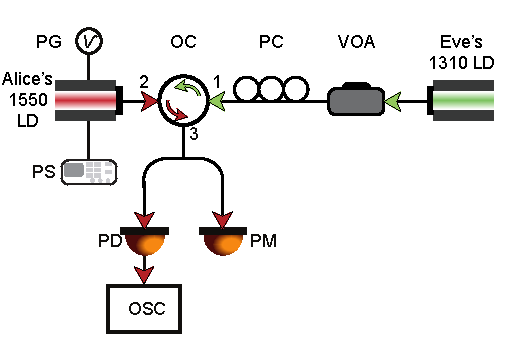
\includegraphics{images/1310 experiment (3).pdf}
    \caption{Экспериментальная установка по проведению атаки оптической накачкой на источник когерентного излучения из состава системы квантового распределения ключей. Alice's LD - лазерный диод Алисы, PG - генератор импульсов, PS - источник напряжения, OC - оптический циркулятор, PC - контроллер поляризации, VOA - перестраиваемый оптический аттенюатор, Eve's LD - лазер Евы, PM - измеритель мощности, PD - фотодиод, Osc - осциллограф. \cite{fadeev2025}}
    \label{fig:ch4 1310 exp}
\end{figure}
Данная схема работает следующим образом. На лазер Алисы (LD1550, Agilecom WSLS-934010C4124-82) подается ток смещения с помощью лабораторного блока питания. Величина тока накачки должна не превышать порогового значения. После этого подаются импульсы с генератора импульсов для работы лазерного диода в режиме переключения генерации. Выход лазерного диода подключен ко 2 выходу оптического циркулятора с сохранением поляризации. В первый же вход циркулятора подается излучение от лазера Евы. Ее лазер также основан на полупроводниковом кристалле с распределенной обратной связью, однако его рабочая длина волны составляет 1310 нм, когда лазер Алисы работает на длине волны 1550 нм. Непрерывное излучение от лазера Евы попадает на переменный оптический аттенюатор (OZ Optics, BB-100) для изменения выходной мощности лазера без изменения тока накачки, увеличение или уменьшение которого приводит к изменению длины волны лазера, что является критичным изменением для повторяемости эксперимента. После этого излучения попадает на механический контроллер поляризации для согласования оси поляризации выходного излучения с осью поляризации оптического циркулятора и лазера соответственно для максимальной эффективности ввода оптического излучения в резонатор лазера Алисы. Попадая на 1 вход оптического циркулятора, излучение Евы проходит его без изменений и с небольшим затуханием попадает в волоконный вывод лазера Алисы. Распространяясь по нему, оно попадает на зеркало кристалла, от которого оно частично отражается, а частично проходит внутрь. Для очистки данных была измерена мощность излучения, отраженного от всех элементов лазера и вычтена из полученных результатов. В результате прошедшее излучение поглощается кристаллом InGaAs и благодаря этому создается дополнительная инверсия населенностей в кристалле, которая повышает выходную мощность лазерного излучения на длине волны 1550 нм. Влияние этого эффекта и рассматривается в данной главе. 
%\section{Изменение Ватт-Амперной характеристики лазера с распределенной обратной связью при атаке на рабочей длине волны}\label{sec:ch4/sect2}

\section{Изменение Ватт-Амперной характеристики лазера с распределенной обратной связью при атаке на других длинах волн}\label{sec:ch4/sect3}
Одной из основных характеристик лазера является его ватт-амперная характеристика. Эта кривая показывает зависимость прироста мощности выходного излучения в зависимости от тока накачки, пропускаемого через кристалл. В рамках данного раздела описывается изменение этой характеристики в зависимости от мощности лазера Евы.
Для этого лазер Алисы работал в непрерывном режиме только с накачкой током от лабораторного блока питания. Мощность контролировалась оптическим измерителем мощности (Thorlabs, PM400). А ток накачки лазера варьировался от 0 до 25 мА. 
Результат измерения данных характеристик представлен на рисунке \ref{fig:Watt-Amp ch4}.
\begin{figure}
    \centering
    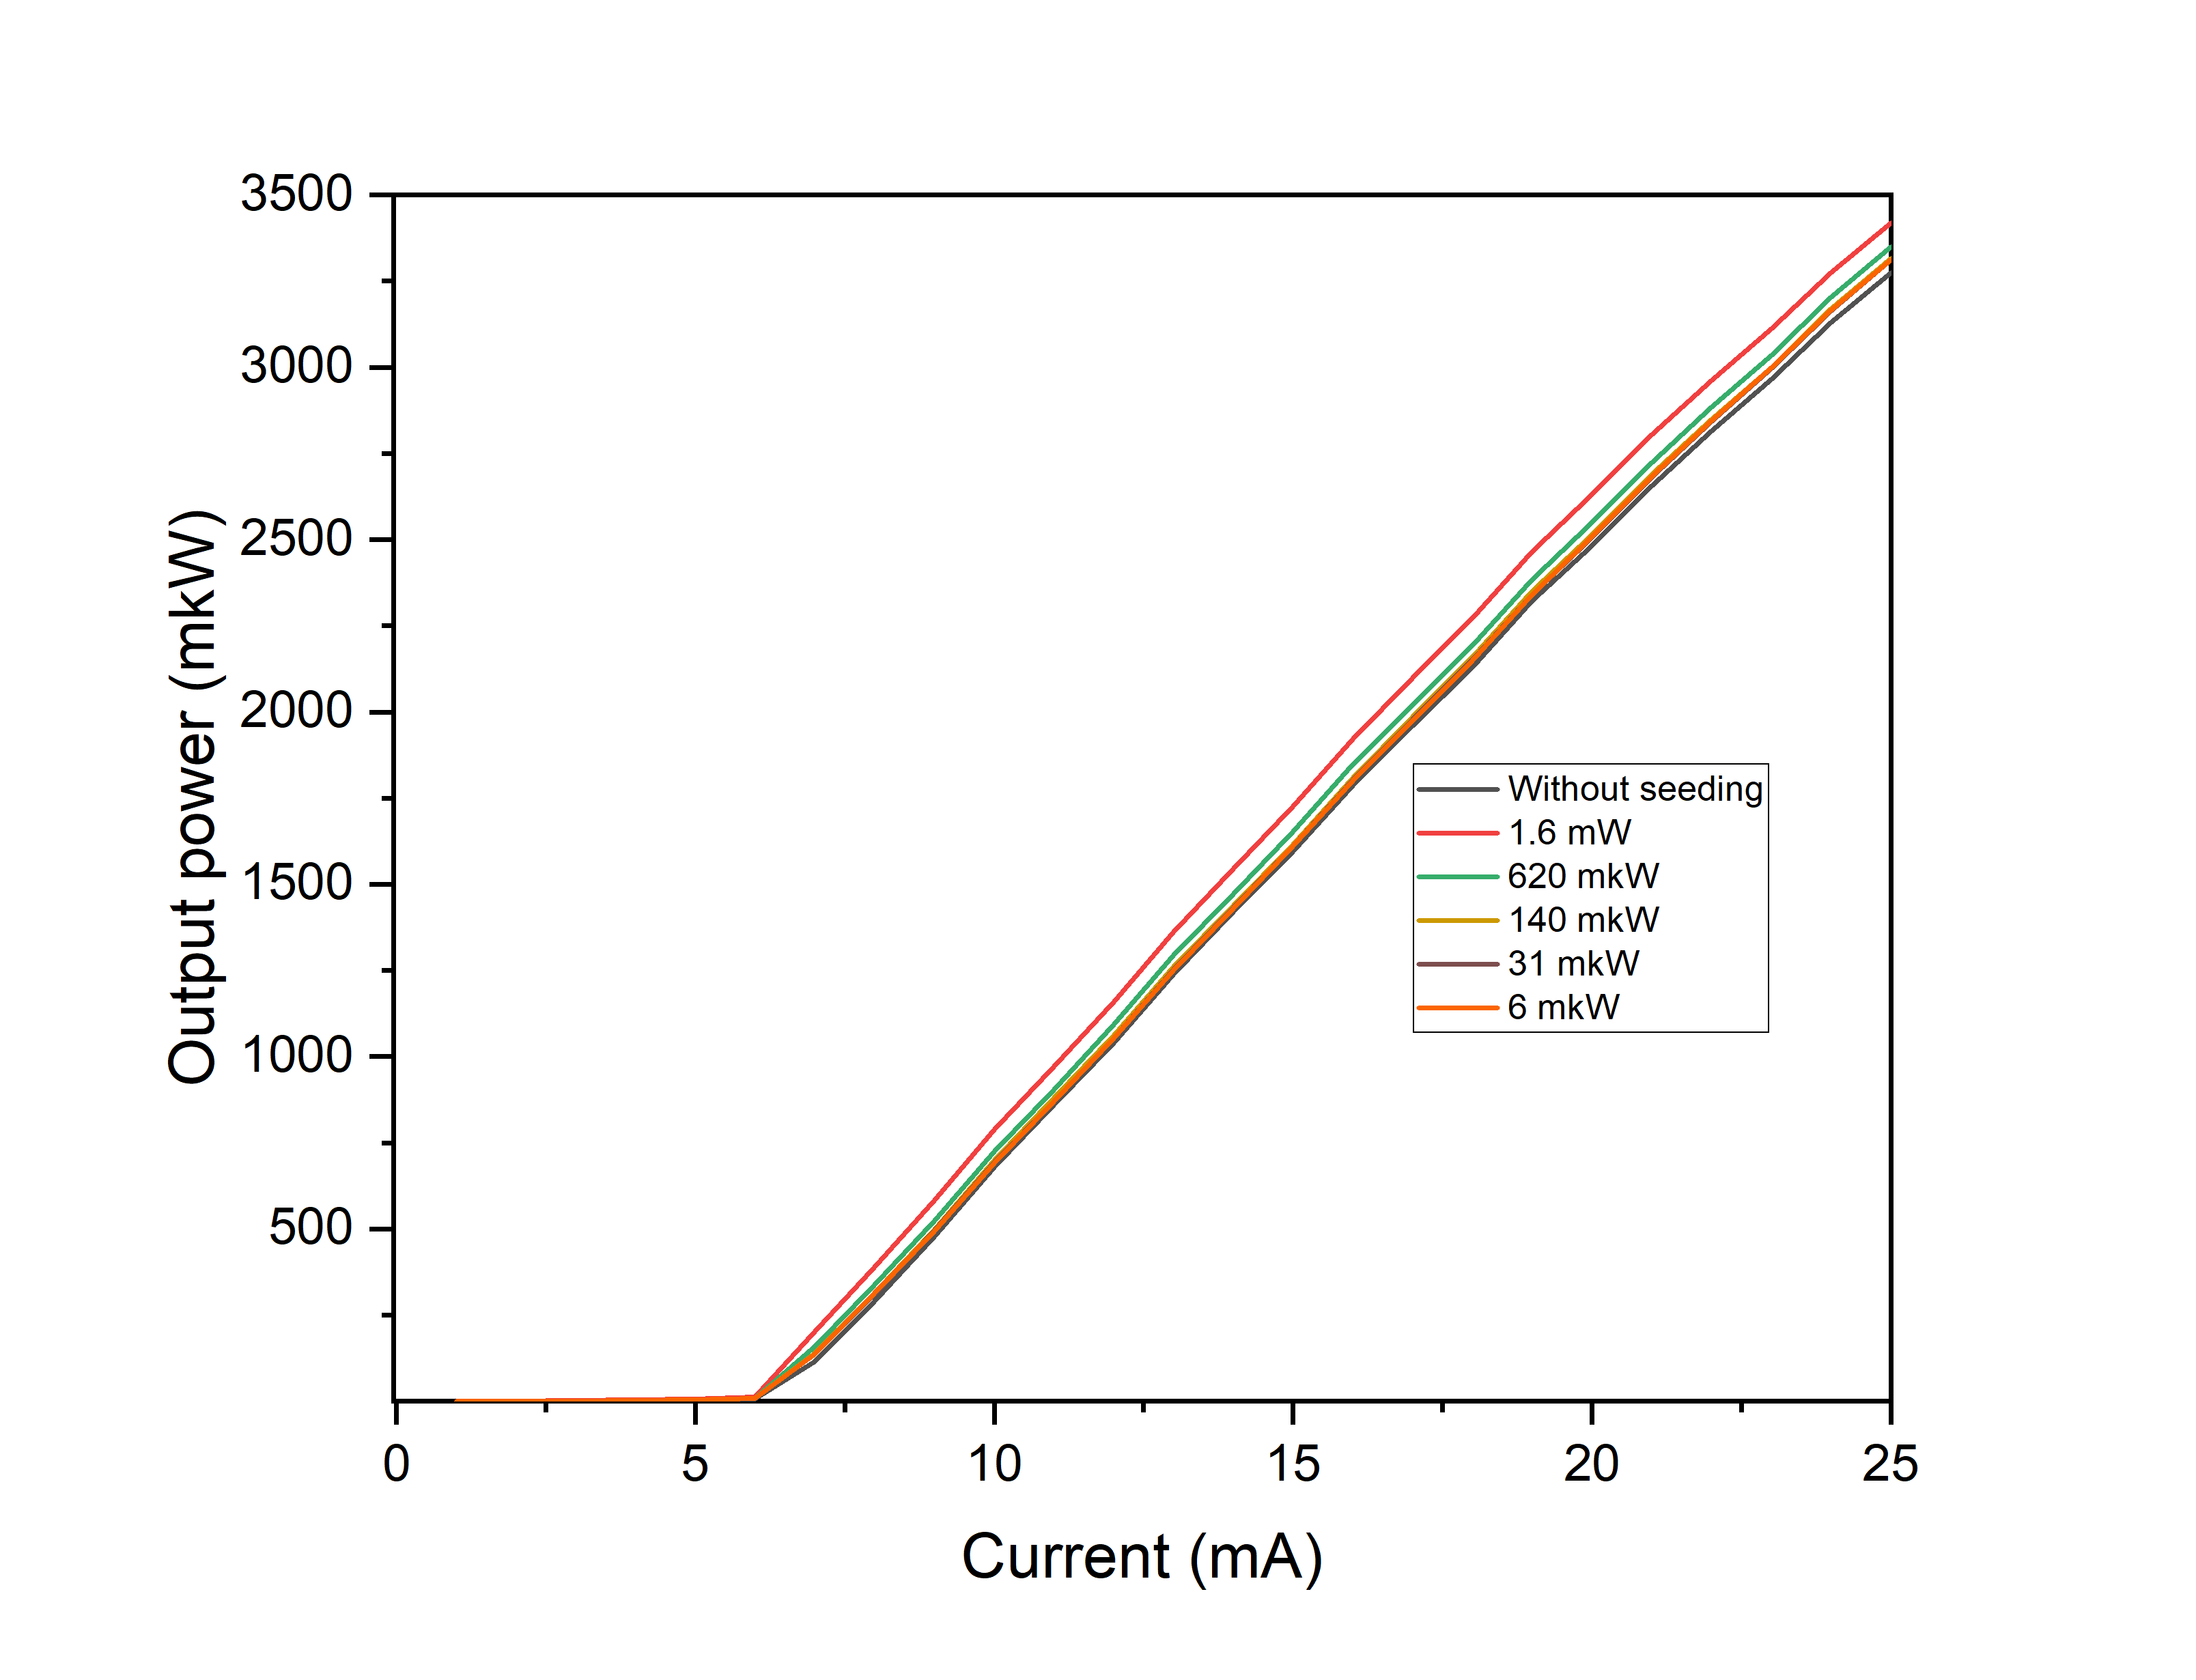
\includegraphics[width=\linewidth]{images/ватт ампер для диссера.png}
    \caption{Ватт-Амперные характеристики лазера Алисы под действием внешней оптической накачки от Евы. \cite{fadeev2025}}
    \label{fig:Watt-Amp ch4}
\end{figure}
Данные графики демонстрируют, что дополнительная накачка от Евы в диапазоне мощностей от 1.6 мВт до 31 мкВт сдвигает исходную Ватт-Амперную кривую, что показывает возможность Евы манипулировать мощностью Алисы. Для численной оценки этого влияния необходимо перейти к дифференциальной квантовой эффективности \cite{cassidy1984,tomiyasu2017}. Эта величина показывает эффективность преобразования электронного тока в фотоны, излучаемые лазером. Формула расчета величины дифференциальной квантовой эффективности ниже 
\begin{equation}
\eta = \frac{2e}{\hbar\omega}\frac{dP}{dI}
\label{eq:quaneff}
\end{equation}, 
где $\eta$ - дифференциальная квантовая эффективность, e - заряд электрона, $\hbar$ - приведенная постоянная Планка, $\omega$ - частота лазера, $dP/dI$ - аппроксимированное значение производной измеренных Ватт-Амперных характеристик.
В результате этих вычислений показано на рисунке \ref{fig:diff quant eff ch4}, что Ева, используя оптическую накачку на 1310 нм, изменяет дифференциальную квантовую эффективность лазера Алисы, что приводит к увеличению выходной мощности лазера при неизменном токе накачки.
\begin{figure}
    \centering
    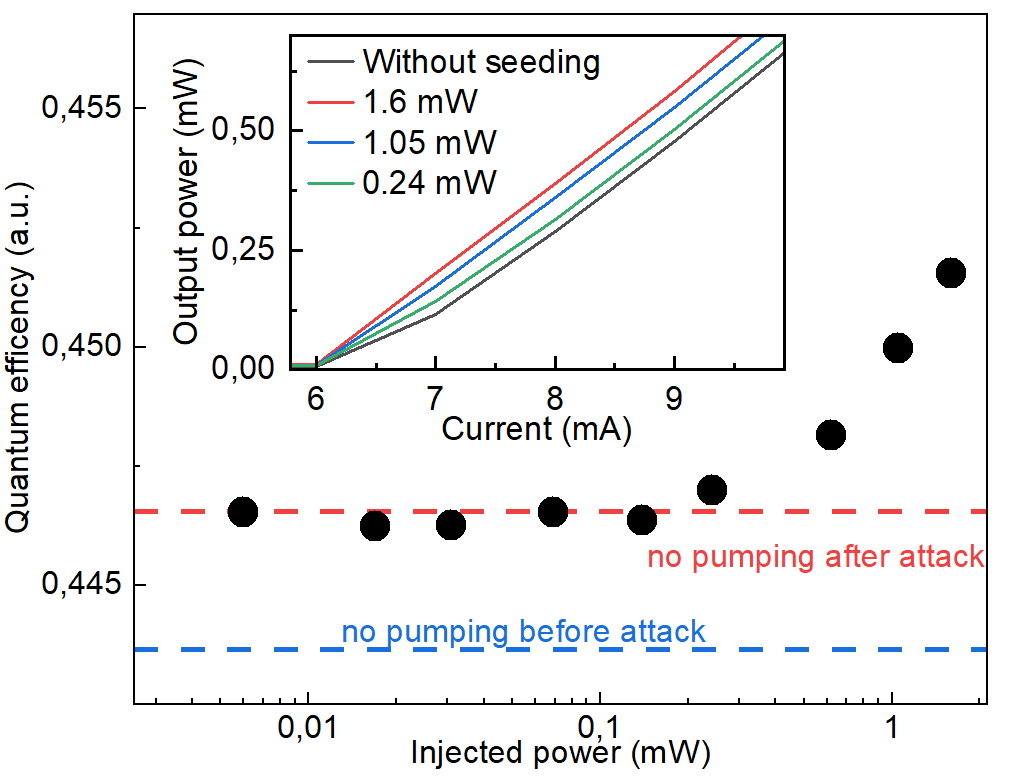
\includegraphics{images/Эффективность 1310.png}
    \caption{График зависимости дифференциальной квантовой эффективности в зависимости от мощности накачки Евы. Красная пунктирная линия обозначает значение дифференциальной квантовой эффективности после проведенной атаки, а синяя пунктирная линия обозначает значение дифференциальной квантовой эффективности до атаки \cite{fadeev2025}}
    \label{fig:diff quant eff ch4}
\end{figure}
В результате аппроксимации наклона ватт-амперных характеристик и расчета дифференциальной квантовой эффективности (ДКЭ) по формуле \ref{eq:quaneff} было показано, что Ева может увеличивать ДКЭ на несколько процентов. Это изменение приводит к тому, что повышается среднее число фотонов, излучаемое Алисой. В результате необходима переоценка скорости выработки секретного ключа из-за увеличения среднего числа фотонов, но этого не происходит, что позволяет Еве перехватывать разницу в ключах и использовать его в своих целях. 

\section{Изменение формы импульса при атаке на лазер с распределенной обратной связью, работающем в режиме переключения усиления}\label{sec:ch4/sect4} 
Для измерения влияния оптической накачки на форму и энергию импульсов, сгенерированных Алисой, необходимо использовать лазер Алисы в импульсном режиме. Для этого атакуемый лазер был переведен в режим работы переключения усиления для генерации импульсов. Ток накачки составил 3 мА. Импульсы же генерировались генератором импульсов (P400, Highland Technology). Полученные импульсы регистрировались опто-электронным конвертором (PDI35-10G, Laserscom) и оцифровывалось осциллографом 735Zi, Lecroy, с полосой пропускания 3.5 ГГц, скорость оцифровки 40 ГС/с. Для синхронизации на осциллограф был дополнительно выведен электрический сигнал с генератора импульсов для запуска развертки и точного измерения времени прихода импульсов. Частота повторения этих импульсов составляла 10 МГц и длительность импульса составляла 700 пс. Результат измерения этих импульсов представлен на рисунке \ref{fig:pulse shape ch4}.
\begin{figure}
    \centering
    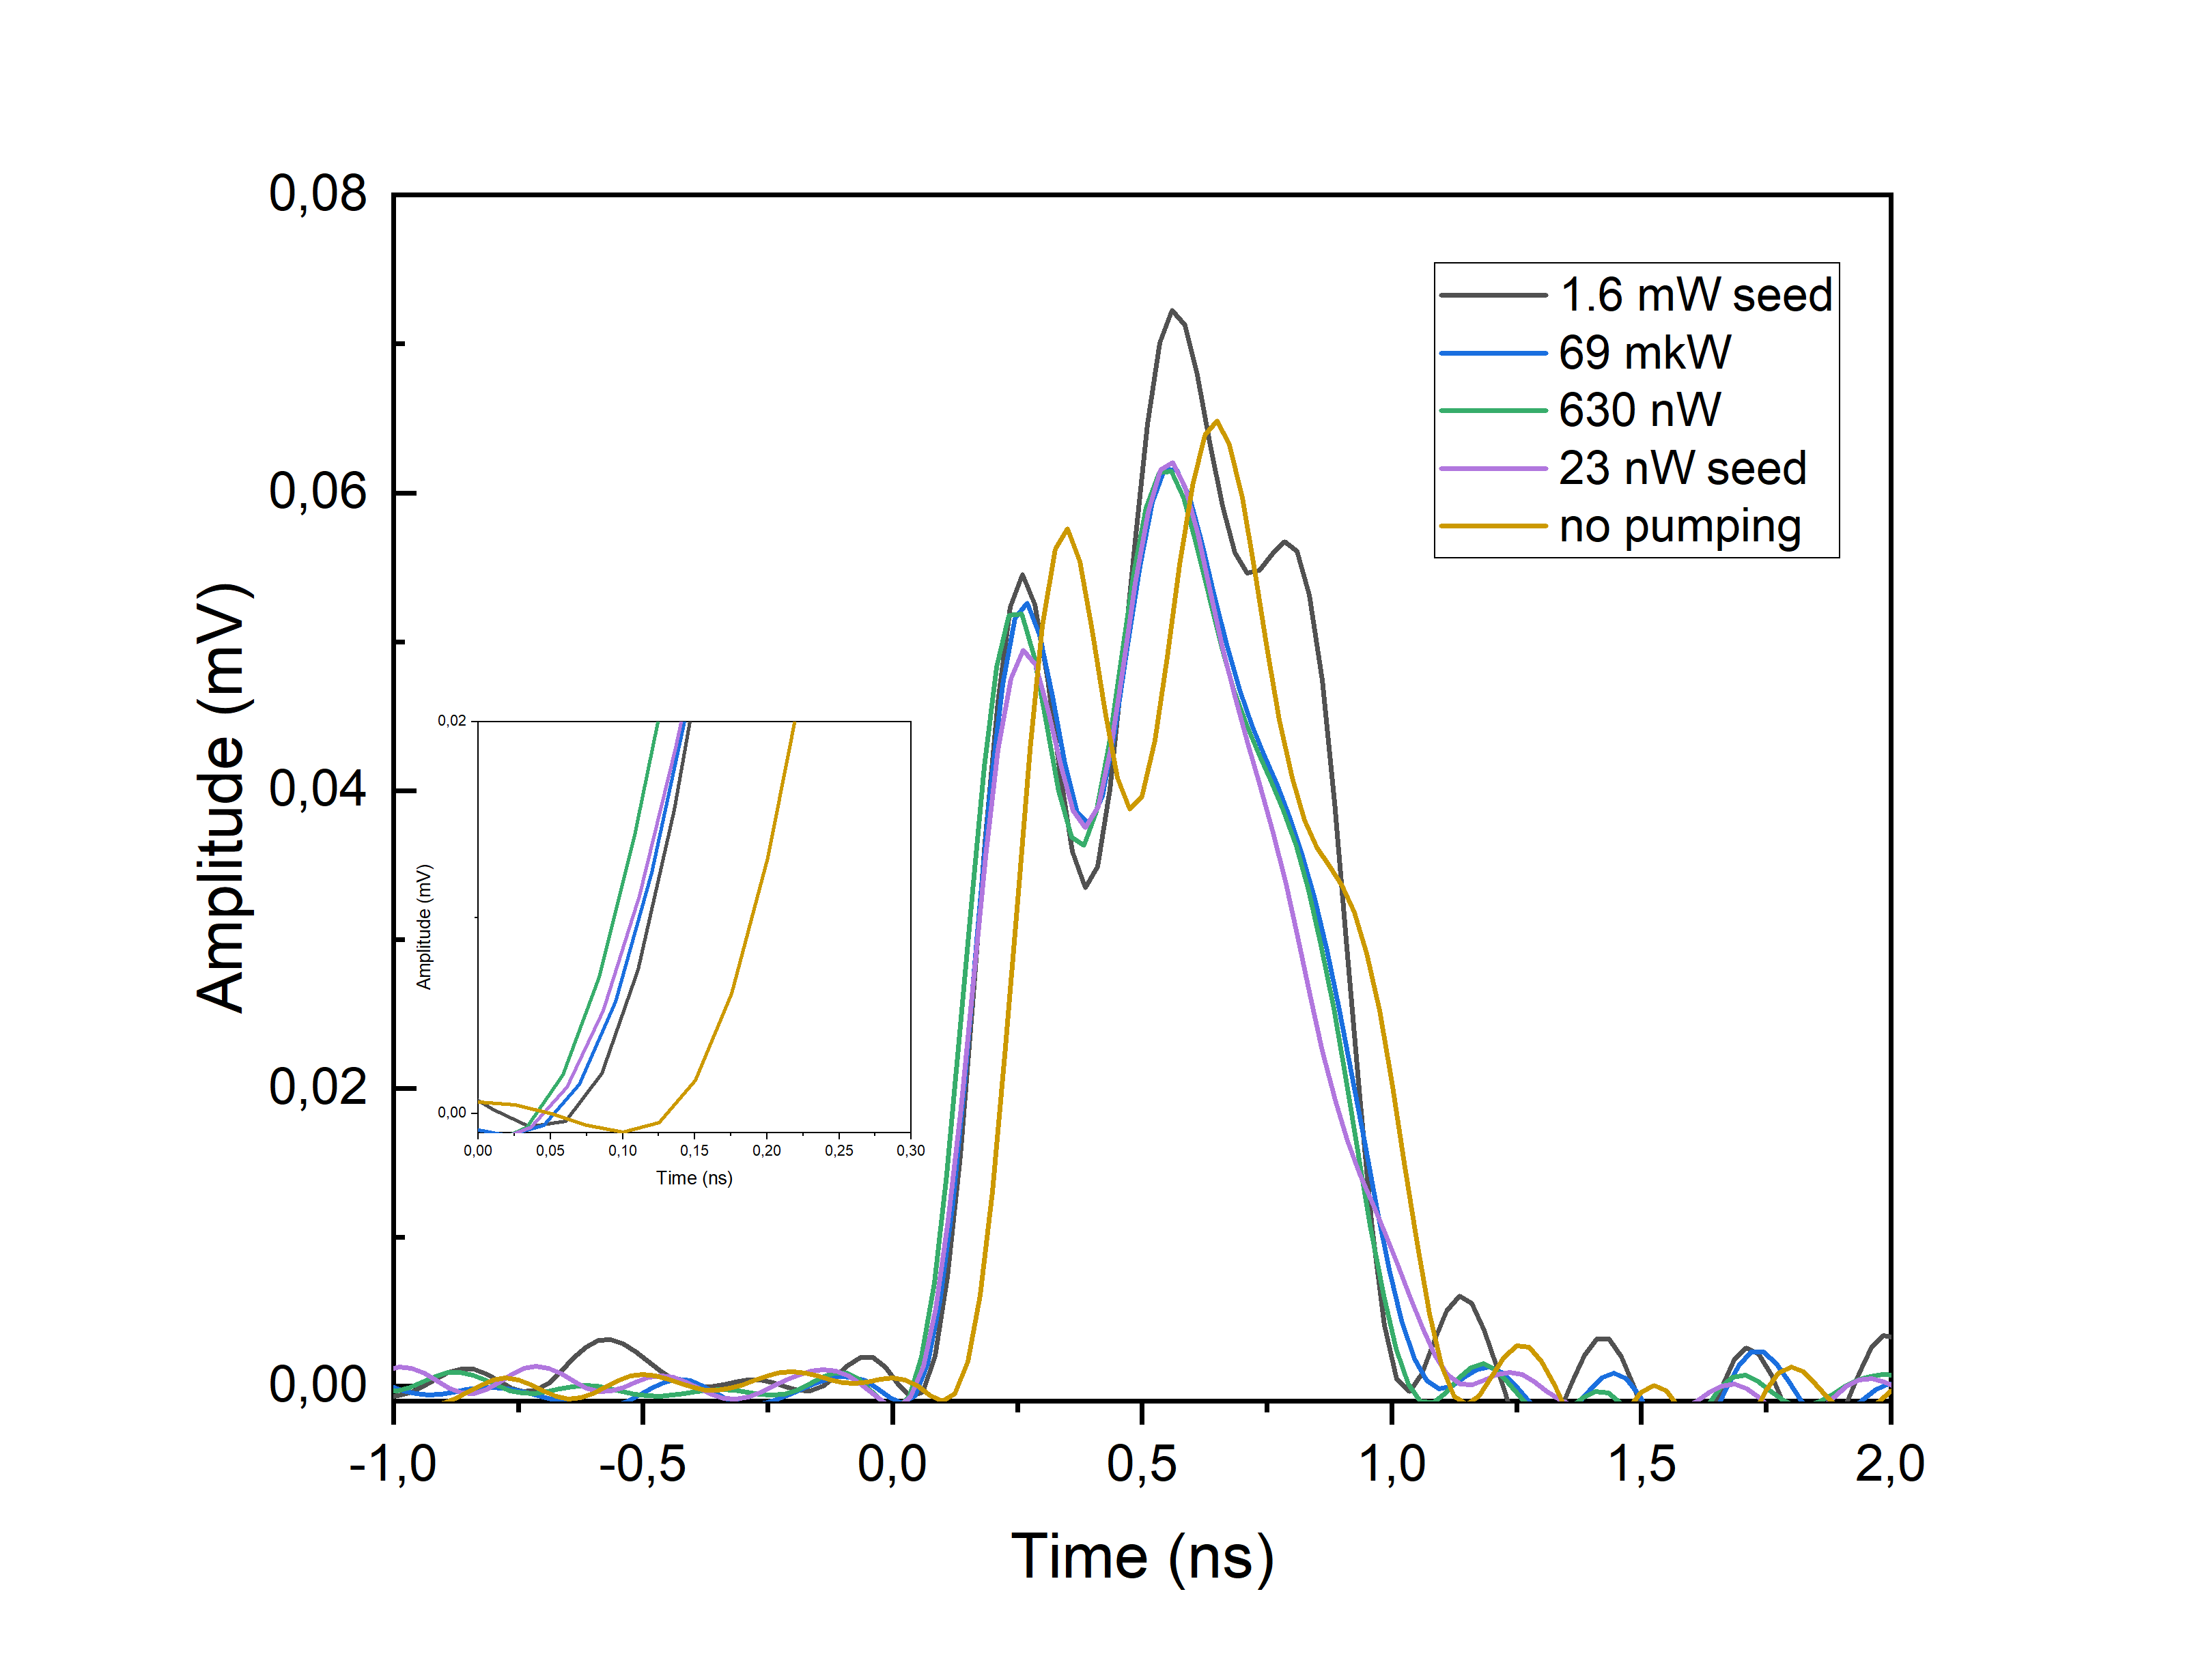
\includegraphics[width=\linewidth]{images/Импульсы под действием 1310 для диссера.png}
    \caption{Формы импульсов, сгенерированных Алисой, под действием оптической накачки и без нее \cite{fadeev2025}}
    \label{fig:pulse shape ch4}
\end{figure}
Как видно из рисунка \ref{fig:pulse shape ch4}, дополнительная накачка Евы не только увеличивает выходную энергию импульсов, а также сдвигает их время генерации на величину приблизительно равной 100 пс. Для оценки влияния оптической накачки на площадь импульсов, исследуемые импульсы были оцифрованы и их площадь была проинтегрирована в программной среде Origin. Результаты этого интегрирования представлены на рисунке \ref{fig:energy 1310 ch4}.
\begin{figure}
    \centering
    \includegraphics[width=\linewidth]{images/1310_энергия.png}
    \caption{Изменение энергии импульсов под действием накачки лазером на длине волны 1310 нм Евы \cite{fadeev2025}}
    \label{fig:energy 1310 ch4}
\end{figure}
Проведенные измерения показывают, что воздействие Евы изменяет не только дифференциальную квантовую эффективность, но и энергию импульсов, излучаемой Алисой, что позволяет также снижать дальность и скорость выработки секретного ключа. В результате воздействия энергия импульсов не только может увеличиться на 10 процентов, но даже может уменьшится при некоторых мощностях оптического излучения накачки.
\newline Для полной картины изменения мощности, излучаемой Алисой под действием оптической накачки злоумышленника, необходимо оценить еще и средний уровень мощности. Для этого используется лазер, работающий в импульсном режиме, как и описано выше, однако мощность измеряется с помощью измерителя оптической мощности (ИОМ). Скорость работы данного ИОМ не позволяет измерить мощность каждого импульса, поэтому он интегрирует всю мощность и импульсную, и непрерывную. Результат измерения показан на рисунке \ref{fig:avg pwr 1310 ch4} 
\begin{figure}
    \centering
    \includegraphics{images/1310_мощность.png}
    \caption{Изменение средней мощности лазера Алисы под действием оптической накачки Евы \cite{fadeev2025}}
    \label{fig:avg pwr 1310 ch4}
\end{figure}
В результате воздействия Евы, мощность лазера с распределенной обратной связью увеличивается на $20\%$, когда как значение энергии импульсов повышается только на 10\%. Что объясняется тем, что Ева также повышает и непрерывное излучение из лазера Алисы.
\section{Определение минимально необходимой изоляции лазерного источника для предотвращения атаки оптической накачкой}\label{sec:ch4/sect5}
В качестве исходной мощности, которая необходима для создания заметного эффекта, определенная по графику \ref{fig:avg pwr 1310 ch4}, составляет 69 мкВт или -11.6 дБм. Существующие на рынке решения предлагают лазеры, способные выдавать 14 Вт или 41.46 дБм мощности на длине волны 1310 нм \cite{grimes2022}.
Для определения изоляции необходимо вычесть из мощности лазера минимально необходимую мощность для создания эффекта по формуле \ref{eq:1310_iso}.
\begin{equation}
\label{eq:1310_iso}
    \alpha_{iso} = P_{laser} - P_{req}
\end{equation}
В результате вычислений величина изоляции, необходимая для предотвращения атаки оптической накачкой составляет 53 дБ. 

\section{Оценка возможности проведения атаки на существующие системы квантового распределения ключей}\label{sec:ch4/sect6}
Современные системы квантового распределения ключей содержат в себе элементы, предназначенные для защиты от различных атак на техническую реализацию. К таким элементам относятся различные пассивные фильтры и изоляторы.
Однако некоторые защитные элементы могут вести себя непредсказуемо для разных длин волн. Эти особенности позволяют злоумышленнику их использовать для получения информации о ключе.
Ярким примером могут служить DWDM (Dense Wavelength Division Multiplexion) фильтры и оптические изоляторы. Их заявленные характеристики соблюдаются только в относительно небольшом диапазоне длин волн.
С изменением зондирующей длиной волны изменяется и величина изоляции, вносимой элементом. Пример этого эффекта отображен на рисунке \ref{fig:isolation_spectrums}
\begin{figure}
    \centering
    \includegraphics[width=\linewidth]{spectra_1310_iso.pdf}
    \caption{Величина изоляции пассивных элементов, используемых в системах КРК. Красным цветом обозначен спектр изоляции DWDM фильтра, серым - одностадийного изолятора, синим - двухстадийного изолятора \cite{fadeev2025}}
    \label{fig:isolation_spectrums}
\end{figure}
Как видно из рисунка \ref{fig:isolation_spectrums}, представленные элементы не вносят существенной изоляции как на рабочей длине волны. К примеру, изоляция одностадийного изолятора на длине волны 1550 нм составляет 30 дБ, а двухстадийного - 40 дБ. Однако на длине волне 1310 нм эти величины составляют 8 и 12.5 дБ соответственно.
Когда DWDM фильтр на длине волны 1310 нм вносит 5 дБ, в то время как на длине волны 1550 нм вносит 30 дБ потерь \cite{ponosova2022}. Таким образом видно, что пассивные элементы не вносят заявленной изоляции и эта лазейка может быть использован злоумышленником.
В качестве схемы КРК будет использоваться схема из работы \cite{makarov2023}. 
\begin{figure}
    \centering
    \includegraphics[width=\linewidth]{Qrate-Alice.pdf}
    \caption{Оптическая схема блока Алиса \cite{fadeev2025}}\label{fig:Alice_qrate}
\end{figure}
Для расчета необходимой минимальной зондирующей мощности необходимо просуммировать все потери, вносимые элементами на длине волны 1310 нм. 
Измеренные значения потерь элементов продемонстрированы в таблице~\ref{tab:isolation1310}
\begin{table}
    \caption{Потери элементов в системе квантового распределения ключей на длине волны 1310 нм}
    \centering
     \label{tab:isolation1310}
\begin{tabular}[t]{lll}
    \hline\hline
    Элемент & Потери, дБ  \\
    \hline
    Встроенный изолятор в лазере &10.5 \\
    Изолятор 1  & 10.56 &  \\
    Изолятор  2 & 16.24 &  \\
    Фиксированный аттенюатор & 19.6  \\
    Переменный аттенюатор & 0.5 \\
    Светоделитель & 23.98 \\
    DWDM1  & 4.08  \\
    DWDM2  & 3.03  \\
    Фазовый модулятор & 4.5  \\
    Модулятор интенсивности & 4.5 \\
    \hline\hline
    \centering
    \end{tabular}
\end{table}

Вычисления производятся по формуле 
\begin{equation}
    \begin{split}
    \alpha_{1310}=\alpha_\text{Iso1} + \alpha_\text{Iso2} + \alpha_\text{Att} + \alpha_\text{VOA1} + 2\alpha_\text{DWDM} +\\
     \alpha_\text{PM} + \alpha_\text{IM} + \alpha_\text{LD},
     \end{split}
    \label{eq:input power}
\end{equation}
где $\alpha_{Iso}$ вносимые потери изолятором на длине волны 1310 нанометров, $\alpha_{att}$, $\alpha_{VOA}$ , $\alpha_{DWMD}$, $\alpha_{PM}$, $\alpha_{IM}$, и $\alpha_{LD}$ вносимые потери компонентов \ref{fig:Alice_qrate}.
Для определения потерь использовались схожие компоненты как в работе \cite{makarov2023}. Раскрывать модели всех элементов не представляется возможным по соображениям конфиденциальности. 
Но эти элементы представляют собой стандартные телекоммуникационные элементы доступные для заказа. Потери на длине волны 1310 нм фиксированного аттенюатора (Thorlabs FA20T) и светоделителя 99:1 (Thorlabs TW1550R1A2) определены в даташите производителем.
Потери фазового модулятора на основе кристалла Ниобата Лития, легированного Титаном, измерялись с помощью лазера, который используется в эксперименте, и измерителем мощности. Потери в модуляторе интенсивности считаем аналогичными.
Остальные же элементы измерялись с помощью источника суперконтиниума и оптического анализатора спектра (HP Hewlett Packard 70004A) по методологии, описанной в \cite{makarov2023}. Потери на изоляторе, встроенном в лазерный диод, считаем аналогичными одностадийному изолятору в 10 дБ.
В итоге изоляция всей системы, изображенной на \cref{fig:Alice_qrate} составляет 97.55 дБ, что существенно превышает минимальное определенное значение в 53 дБ. Поэтому данная система устойчива к атаке оптической накачкой. 


\section{Выводы по главе}\label{sec:ch4/sect7}
В данной главе рассматривается новый тип атаки на источники лазерного излучения - атака оптической накачкой, на примере накачки на длине волны 1310 нм. Однако, данный эффект наблюдается в широком диапазоне длин волн, обусловленном шириной полосы поглощения полупроводникового кристалла, на котором построен DFB лазер. 
Изучено влияние на интенсивность излучаемой мощности, определена минимально необходимая мощность для создания заметного эффекта в 69 мкВт. Определена минимально необходимая изоляция для предотвращения атаки оптической накачкой на длине волны 1310 нм и зондирующей мощности 14 Вт в 53 дБ.
Определена стойкость существующей системы квантового распределения ключей к атаке оптической накачкой. Ее суммарная изоляция составила 97.55 дБ, что превышает минимальное пороговое значение в 53 дБ, что делает данную систему устойчивой к атаке оптической накачкой. 
           % Глава 4
\chapter{Исследование источника когерентного излучения на основе оптической инжекции на устойчивость к лазерному засеиванию мощным излучением}\label{ch:ch5}
\section{Введение}
На данный момент в практических системах квантового распределения ключей в качестве источника одиночных фотонов используется ослабленный лазерный источник. Это открывает для подслушивающего устройства множество возможностей атаковать источник КРК и получить информацию о секретном ключе. Обычно в качестве контрмеры против атак на источник света КРК рекомендуется использовать некоторую степень изоляции. Однако практические оптические компоненты также могут изменять значение изоляции при внешнем воздействии или под влиянием условий окружающей среды. В данной работе продемонстрировано, что источник лазерного излучения на основе лазерной инжекции обладает очень высокой устойчивостью к атакам внешним засевом, и рекомендуется использовать эту схему в качестве безопасного источника фотонов для систем КРК.
Квантовое распределение ключей (КРК) позволяет двум сторонам распределять секретный ключ по ненадежному каналу, используя квантово-механические свойства одиночных фотонов. Протоколы КРК в принципе не поддаются взлому. Однако их практическая реализация демонстрирует длинный список побочных каналов, которые могут предоставить подслушивающему лицу дополнительную информацию о секретном ключе и сделать систему, использующую его, небезопасной~\cite{sun2022, makarov2023}. Такие побочные каналы почти всегда являются результатом отличия аппаратного обеспечения от его идеальной модели. 

Одним из наиболее ярких примеров несовершенных устройств являются практические источники фотонов. На сегодняшний день в практических системах КРК используются сильно ослабленные лазерные импульсы от полупроводниковых лазерных диодов (ЛД), а не истинные однофотонные источники, поскольку последние пока не позволяют достичь практической скорости передачи ключей ~\cite{zahidy2024}.
Однако, поскольку полупроводниковые лазеры очень чувствительны ко внешним воздействиям, существует несколько атак с лазерной заливкой, которые открывают лазейки для подслушивающих~\cite{huang2019, pang2020, lovic2023}. Например, предыдущие экспериментальные исследования показали, что мощности инжекции в диапазоне 100 - 160 нВт может быть достаточно для управления интенсивностью импульсов Алисы~\cite{huang2019, pang2020}, а мощности даже около 1 нВт может быть достаточно для частичного управления фазой импульсов Алисы~\cite{lovic2023}.

В этой работе обращается внимание на то, что описанные выше атаки с лазерным засевом относятся к источнику света, основанному на одном лазерном диоде с усилением. В то же время, ЛД источники с оптической инжекцией стали широко использоваться в квантовой криптографии, особенно в реализациях квантового распределения ключей, не зависящих от измерительных приборов (MDI КРК)~\cite{wei2020,woodward2021}.

Схема с оптической инжекцией незаменима для приложений, требующих высокой видности интерференции между независимыми лазерными источниками. Техника инжекции света значительно улучшает интерференцию за счет низкого джиттера времени импульса и синхронизации частотных чирпов при сохранении случайности фазы излучаемых лазерных импульсов~\cite{comandar2016}. Более того, последние исследования показывают, что лазерный источник с оптической инжекцией позволяет уменьшить флуктуации интенсивности и тем самым увеличить безопасную скорость передачи ключей при реализации техники состояний-ловушек~\cite{xie2019}. %\AP{add ref}%
 
К сожалению, конфигурация источника с инжекционной блокировкой ранее не тестировалась на устойчивость к атакам с лазерным посевом. В этой работе мы впервые исследуем ее оптические характеристики при внешней лазерной атаке и проводим анализ защищенности при наличии изменений выходного сигнала. В работе показано, что конфигурация источника фотонов с внутренним засевом является эффективной контрмерой против известных атак на источник фотонов КРК. Между тем, наше исследование демонстрирует и другие эффекты, которые могут иметь место только в исследуемой конфигурации источника. В частности, ведомый лазер действует как ненасыщенный оптический усилитель. Это приводит к независимому усилению сигналов ведущего и Евы и позволяет злоумышленнику извлечь дополнительную информацию о секретном ключе
\begin{figure*}
\includegraphics{images/StabilityDiagramsFreq.pdf}
\caption{Карта фазовой синхронизации двух лазеров(область стабильной синхронизации обозначена синим).}
\label{fig:injection}
\end{figure*}
\section{Теоретическое описание метода оптической синхронизации}
\label{sec:theory}

\subsection{Полупроводниковые источники света с инжекционной синхронизацией}

Фазовая синхронизация с помощью оптической инжекции - это метод оптической частотной и фазовой синхронизации, основанный на освещении лазерного резонатора внешним светом. Источник с оптической инжекцией содержит "ведущий" лазер, который обеспечивает внешнее излучение для воздействия на "ведомый" лазер~\cite{liu2020}. 

В зависимости от интенсивностей и спектральных показателей ведущего и ведомого ЛД, источник может обеспечивать режим свободной генерации, стабильной или нестабильной синхронизации~\cite{lau2008}. Эти режимы определяются как области диаграммы с коэффициентом инжекции и частотной подстройкой в виде координат, как показано на \cref{fig:injection}. Частота перестройки - это разность между частотами ведущего и свободно работающего ведомого каналов. Коэффициент инжекции $R_I$ определяется как 

\begin{equation}
\label{eq:injection_coeffitient}
	R_I = -10\times\lg\left({\frac{Q_c^M}{Q_c}} \right),
\end{equation}
%
где $Q_c^M$ и $Q_c$ значения интенсивности ведущего и ведомого лазеров в режиме свободной генерации в установившемся режиме, соответственно.
Отметим также, что в импульсном режиме работы ЛД интенсивности $Q_c^M$ и $Q_c$ определяются пиковыми мощностями импульсов как 
\begin{equation}
\label{eq:intens}
	Q = \frac{<P>}{f_R\times\tau_P},
\end{equation}
где $<P>$ - средняя мощность в Ваттах, $f_R$ - частота повторения импульсов, Гц, и $\tau_P$ - длительность импульса, с.
\begin{table}
	\caption{Параметры лазера для создания оптической инжекции} 
	\label{tab:sim_param}
	\begin{tabular}[t]{@{\extracolsep{1.8ex}}l@{}c@{\quad}l@{}c@{}}
		\hline\hline
		Параметр		&Значение  			&Параметр 	& Значение	\\ 
		\hline
		$N_{th}$		&$5.5\times10^7$ 	&$N_{tr}$  		& $5.0\times10^7$		\\   
		$\tau_{e}$		&$1~ns$	&$\tau_{ph}$ 	&$1~ps$		\\ 
		$C_{sp}$		&$10^{-5}$ 		& $\Gamma$	& 0.12				\\
		$\alpha$		&5 				& $\kappa_{inj}$	& $5.0\times10^{10} ns^{-1}$	\\  
		I			&$22~mA$	& $\gamma_Q$	& 0				\\
		\hline\hline
	\end{tabular}
	\label{tab:all}
\end{table}
Когда источник работает в режиме стабильной синхронизации, ведомый лазер будет вынужден синхронизироваться с ведущим, то есть излучать на той же частоте. В целом, согласно карте синхронизации на рисунке \ref{fig:injection}, диапазон синхронизации частоты становится больше с увеличением коэффициента инжекции~\cite{wang2013}. Между тем, в практических источниках света для систем КРК коэффициент инжекции отрицательный. Низкий коэффициент инжекции обусловлен двумя факторами. Во-первых, излучение ведущего не полностью заходит в резонатор ведомого. А второй фактор связан с длительностью импульса в соответствии с \cref{eq:intens}. Широко используемый случай реализации оптической схемы предполагает длительность импульса ведомого лазера в несколько раз меньше, чем у ведущего ЛД (в два раза и больше). Это позволяет избежать высокоамплитудных релаксационных осцилляций в выходных импульсах за счет засева ведомого лазера только частью импульса без частотного чирпа по интенсивности ведущего. В итоге, для получения высокой стабильности интенсивности исследуемых источников ведущий и свободно работающий ведомый ЛД должны иметь как можно более близкую рабочую длину волны.

%\subsection{Многоволновое усиление в полупроводниковых усиливающих средах}

%Традиционно полупроводниковые источники с оптической инжекцией включают в себя два лазера, ведущий и ведомый лазерные диоды, и теоретически они изучаются в рамках концепции этой конструкции. Однако в этом разделе мы также хотели бы рассмотреть это явление в аспекте усиления излучения в ведомом лазере. Это необходимо для понимания анализа экспериментальных результатов и атак на источник КРК с оптической инжекцией. Конструкции волноводов и материал усиления одинаковы или похожи для лазерных диодов и полупроводниковых оптических усилителей (ПОУ). Разница в том, что в лазерах для генерации и поддержания колебаний вокруг среды усиления формируется резонатор, и сигнал проходит несколько кругов внутри резонатора перед выходом~\cite{chen2022}. Поэтому предположим, что ведомый лазер - это двухпроходной ПОУ с неидеальным входом, который дает отражения
\subsection{Статистика интерференции фазово-рандомизированного классического света}

Статистические свойства интерференционного сигнала фазово-рандомизированного классического света хорошо изучены и имеют строгие модели, учитывающие все характеристики импульсов~\cite{shakhovoy2020, shakhovoy2021}. Недавно они были разработаны для реализации высококачественных квантовых генераторов случайных сигналов, основанных на интерференции фазово-рандомизированных импульсов. Благодаря этому, используя функцию плотности вероятности интерференционного сигнала, можно дать оценку видимости интерференции, объяснить влияние на нее свойств импульса и, наконец, что очень важно, настроить источник света так, чтобы получить наибольшую видимость интерференции. Поэтому в наших экспериментах мы не измеряем двухфотонную интерференцию, а измеряем и анализируем функцию плотности вероятности интерференции классического света. 

Процедура состоит в следующем. Она включает в себя реализацию несимметричного интерферометра с линией задержки, обеспечивающей время задержки, кратное периоду повторения импульсов. Это приводит к интерференции между импульсами, испускаемыми в разное время. Далее с помощью осциллографа накапливается большая выборка измерений площади интерференционного сигнала и строится гистограмма зависимости числа импульсов от их площади.

В работе~\cite{shakhovoy2021}, авторы показали, что безщелевой колоколообразный лазерный импульс будет иметь двухпиковую форму PDF, где пики будут располагаться на интенсивности конструктивной и деструктивной интерференции, как показано на~\cref{fig:PDF}.
\begin{figure}
\includegraphics[width=\linewidth]{PDF}
\caption{Нормализованная функция плотности распределения интерференции колоколообразных импульсов без чирпа~\cite{shakhovoy2021}.}
\label{fig:PDF}
\end{figure}
Чтобы сравнить функции плотности распределения (ФПР) друг с другом, введем экспериментальную видимость интерференции
\begin{equation}
\label{eq:visibility}
	\eta = {\frac{S_{max} - S_{min}}{4\sqrt{s_1 s_2}}},
\end{equation}
где $S_{max}$ и $S_{min}$ - нормированные интенсивности конструктивной и деструктивной интерференции, определяемые по максимальным экспериментальным вероятностям, $s_1$ и $s_2$ - интенсивности начальных импульсов, которые принимаются равными 1.
\section{Проведение эксперимента}
\label{sec:experiment} 

На рисунке \Cref{fig:setup} показана экспериментальная установка. Она включает в себя три основные части. Это источник света Алисы, атакующий лазер злоумышленника и измерительное оборудование.
\begin{figure}
\includegraphics[width=\linewidth]{setup}
\caption{Экспериментальная установка (PM-волокна выделены красным цветом): VOA - перестраиваемый оптический аттенюатор, BS - светоделитель, PMCIR - циркулятор с сохранением поляризации, PMBS - светоделитель с сохранением поляризации, PG - генератор импульсов, OPM - измеритель оптической мощности, OSC - осциллограф, OSA - оптический анализатор спектра, BS - светоделитель, LT - световая ловушка, FM - зеркало Фарадея. Коэффициент связи светоделителя (BS) обозначается 99 =: 1× означает, что $99\%$ света проходит в порт, горизонтально противоположный графическому обозначению СД, в то время как $1\%$ света
свет попадает в другой порт}.
\label{fig:setup}
\end{figure}
\subsection{Источник света на испытаниях}

В этой работе реализован оптический источник излучения с оптической инжекцией. Его оптическая схема обозначена как Alice в \cref{fig:setup}. Ведущий лазер излучает импульсы со случайной фазой. Они поступают в ведомый лазер через волоконно-оптический циркулятор PMCIR1 (PMCIR-3-A-1550-900-5-08-FA, Optel) из порта~1 в порт~2 и ``засевают'' ведомый лазер. Далее импульсы от ведомого ЛД передаются из порта~2 циркулятора на выход Алисы - порт~3 циркулятора.

В качестве источника мы использовали пару идентичных волоконно-оптических DFB лазерных диодов с выходным волокном, сохраняющим поляризацию (Agilecom, WSLS-934010C4124). Они отличаются только наличием встроенного изолятора. У ведущего лазера он есть, а у ведомого - нет. Чтобы избежать нежелательной обратной связи в ведущем лазере с ведомым, ведущий ЛД дополнительно защищен с помощью внешнего волоконно-оптического изолятора (с изоляцией около 60 дБ, не показан в~\cref{fig:setup}). Отметим, что PMCIR1 также обеспечивает изоляцию порта~2 от порта~1 более чем на 40 дБ. В сумме, с учетом типичной изоляции встроенного изолятора около 30 дБ, ведущий лазер изолирован от ведомого лазера более чем на 130 дБ.
 
На лазерные диоды подается ток смещения от лабораторного источника питания (E3648A, Keysight) с напряжением смещения около 1.2-1.4 В и током 2-4 мА. Для получения оптических импульсов с частотой повторения 10.035 МГц ведущий и ведомый лазерные диоды управляются по отдельности двумя цифровыми генераторами задержки и импульсов (P400, Highland Technology). Электрические импульсы подаются в виде прямоугольников с амплитудой - 5 В и длительностью 2.7 нс и 1.9 нс для управления ведущим и ведомым лазерами, соответственно. Для идеальной формы импульса время прихода ведущего импульса на ведомый диод должно быть немного раньше, чем электрический импульс привода ведомого. Такое согласование времени было достигнуто точной настройкой времени задержки между ГС с разрешением задержки 1 пс. Время задержки для ведомого лазера составило 7.6 нс
\begin{figure}
	\centering
	\includegraphics[width=\linewidth]{spectra}
	\caption{Спектры лазерных диодов ведущего, ведомого и источника излучения для КРК}
\end{figure}\label{fig:QKD_source_spectra}

\begin{figure}
	\centering
	\includegraphics[width=\linewidth]{envelope}
	\caption{Формы импульсов лазеров мастера, слейва и источника излучения КРК}
\end{figure}\label{fig:QKD_source_pulse}
%\caption{Spectral characteristics~(a) and pulse envelope~(b) of the master, slave LDs, and adjusted QKD source.}
%\label{fig:QKD_source}

Согласование спектральных характеристик ведущего и ведомого лазеров достигается путем температурной подстройки ЛД с помощью встроенных термоэлектрических элементов. Фактическая частота отстройки, определяемая как разница между пиковыми частотами ведущего и свободно работающего ведомого, составляет менее 6 ГГц. На рисунках \ref{fig:QKD_source_spectra} и \ref{fig:QKD_source_pulse} показаны спектральные характеристики и огибающую импульса ведущего ЛД, свободно работающего ведомого ЛД (без сигнала от ведущего ЛД) и всего источника света (ведомый ЛД, засеянный ведущим ЛД) после настройки. 

Максимальная средняя мощность ведущего лазера на входе в ведомый ЛД составляет 11 мкВт. Чтобы избежать изменения спектральных характеристик при изменении мощности ведущего лазера, она изменяется с помощью микроэлектромеханического переменного оптического аттенюатора VOA (V1550PA, Thorlabs). Управляющее напряжение VOA от 0 до 5 В контролирует затухание, которое может быть увеличено до 25 дБ с помощью напряжения. 

\subsection{Экспериментальная установка}

Наша экспериментальная установка моделирует сценарий, в котором Ева атакует источник QKD из квантового канала. Из-за наличия волоконно-оптического циркулятора в схеме источника Алисы, свет злоумышленника может воздействовать только на ведомый лазер; типичная конструкция волоконно-оптического циркулятора не позволяет свету передаваться от порта 3 циркулятора к порту 1.

В качестве начального лазера злоумышленника мы использовали лазерный диод с распределенной обратной связью (Gooch and Housego AA1406), усиленный волоконным усилителем на основе легированного эрбием и иттербием волокна (EDFA, заказной блок QGLex)\cite{huang2020}. Он работает в непрерывной генерации на рабочей длине волны в диапазоне от 1548.6 до 1550.6 нм. Применяемая в экспериментах мощность составляет около 500 мВт, поскольку дальнейшее увеличение мощности приводит к изменению вносимых потерь и изоляции циркулятора Алисы PMCIR1. Установка Евы также оснащена делителем луча 99:1 и мониторным измерителем оптической мощности, позволяющим измерять мощность Eve в режиме онлайн. Механический регулятор поляризации установлен для достижения минимальных потерь для света злоумышленника в установке. Свет злоумышленника поступает в источник Алисы через сохраняющий поляризацию волоконно-оптический циркулятор PMCIR2 (PMCIR-3-A-1550-900-5-08-FA, Optel). Далее, прежде чем попасть на целевой ведомый лазер, он проходит в обратном направлении циркулятора Алисы PMCIR1, что обеспечивает изоляцию для света злоумышленника примерно в 46-51 дБ . В результате мощность атакующего лазера, достигающая ведомого лазера Алисы, составляет около 1.8 мкВт .

Конфигурация измерений позволяет контролировать среднюю мощность, спектральные, амплитудно-временные характеристики импульсов и интерференцию следующих друг за другом импульсов. Средняя мощность измеряется с помощью оптического измерителя мощности OPM (S154C, Thorlabs). Выходные спектры измеряются оптическим анализатором спектра OSA (AQ6370D, Yokogawa) со спектральным разрешением 0.02 нм. Амплитуда, длительность импульсов, их стабильность и интерференционные сигналы измеряются осциллографами OSC1 и OSC2 (735Zi, Lecroy, полоса пропускания 3.5 ГГц) и p-i-n фотодиодами (PDI35-10G, Thorlabs) с полосой пропускания 10 ГГц. Для анализа статистических распределений амплитуды и длительности оптических импульсов для каждого измерения накапливается 30 тыс. выборок и строится стандартное отклонение. Затем из средних значений амплитуды и длительности и их стандартных отклонений рассчитываются энергия импульса и его стабильность соответственно.
\begin{figure}
	\centering
	\includegraphics[width=\linewidth]{images/master_power.pdf}
	\caption{Зависимость мощности ведущего лазера (черный) и коэффициента инжекции(красный) от напряжения на аттенюаторе.}
\end{figure}
\label{fig:master_power}
\begin{figure}
	\centering
	\includegraphics[width=\linewidth]{images/hist_initial.pdf}
	\caption{Функции плотности вероятности интерференции импульсов источника КРК под действием различной мощности лазера-ведущего}
\end{figure}
\label{fig:QKD_PDF}
\begin{figure}
	\centering
	\includegraphics[width=\linewidth]{images/spectra_att.pdf}
	\caption{Спектры излучения лазера-ведомого под действием переменных мощностей лазера-ведущего}
\end{figure}
\label{fig:QKD_spectr}

\begin{figure}
	\centering
	\includegraphics[width=\linewidth]{images/envelope_att.pdf}
	\caption{Формы импульсов лазера-ведомого под действием различных мощностей лазера-ведущего}
\end{figure}
%\caption{Характеристики источника QKD в зависимости от напряжения на аттенюаторе: средняя мощность ведущего волокна на входе ведомого волокна (PMCIR1, порт~2) и коэффициент инжекции (a), функция плотности вероятности сигнала помехи (b), выходные спектры (c) и огибающая импульса (d).}
\label{fig:QKD_att}

В наших экспериментах мы анализируем качество импульсов, основываясь на форме функции плотности вероятности интерференционного сигнала, как это описано в \cref{sec:theory}. Чтобы обеспечить интерференцию между следующими друг за другом импульсами, мы реализуем полностью волоконный интерферометр Майкельсона на зеркалах Фарадея и с линией задержки длиной около 10 метров. Затем, 20 тысяч измерений площади интерференционного сигнала накапливаются в фиксированном временном интервале (синхронизированном с электрическими импульсами ЛД) для построения гистограммы с помощью встроенного осциллографа.

Во-первых, мы полностью охарактеризовали источник КРК для различных мощностей ведущего ЛД и экспериментально определили границы мощности ведущего ЛД, необходимые для стабильной оптической инжекции. Далее мы провели серию экспериментов по внешней лазерной атаке на Алису и получили зависимости всех характеристик КРК-источника от средней мощности ведущего ЛД. И, наконец, мы исследовали выходные спектры КРК под воздействием внешнего излучения с различной рабочей длиной волны.
\section{Результаты экспериментов}
\label{sec:results}

\subsection{Характеристики источника КРК}

%\Cref{fig:QKD_att} иллюстрирует характеристики источника КРК в зависимости от напряжения управления аттенюатором.

Средняя мощность ведущего ЛД на втором порту PMCIR1 изменяется от 11 до 0.12 мкВт при увеличении напряжения VOA до 4 вольт. Рисунок \Cref{fig:master_power} демонстрирует эту зависимость и соответствующий расчетный коэффициент инжекции без учета потерь на сопряжении полупроводникового материала с оптическим волокном внутри ведомого лазера (в зависимости от внутренней конструкции ЛД, он может находиться в диапазоне от 1 до 10 дБ). 

Чтобы определить диапазон, в котором ведомый ЛД синхронизируется с излучением ведущего, мы измерили и проанализировали функцию плотности распределения интерференции следующих друг за другом импульсов, спектральные и время-амплитудные характеристики выходных импульсов для каждой мощности ведущего ЛД, построенные на рисунке \cref{fig:master_power}. ФПР, измеренные для различных мощностей ведущего ЛД на рисунке\cref{fig:QKD_PDF}, показывают, что синхронизация происходит, когда мощность ведущего ЛД находится в диапазоне от 2.29 до 11 мкВт. Форма ФПР имеет два пика, соответствующих идеальной конструктивной и деструктивной интерференции. При мощности основного ЛД 0.69 мкВт видность интерференции ухудшается. И, наконец, при минимальной мощности ведущего 0.12 мкВт, ФПР имеет только один высокий пик в центре. Это означает, что ведомый не имеет оптической синхронизации с ведущим. Без синхронизации временной джиттер импульсов увеличивается, что приводит к увеличению вероятности отсутствия помех.

Из спектров \Cref{fig:QKD_spectr} и измерений огибающей импульсов \cref{fig:QKD_att} также видно, что ведомый ЛД не синхронизируется с излучением ведущего на 0.12 мкВт. В этом случае длина волны выходного сигнала отличается от длины волны ведущего, а также форма выходного импульса далека от идеальной колоколообразной формы, на нее влияют релаксационные осцилляции. В ``граничном'' состоянии при мощности ведущего излучения 0.69 мкВт релаксационные колебания в форме импульса отсутствуют, в то же время его спектр имеет второй интенсивный пик, по частоте отличающийся от частоты ведущего ЛД.

\subsection{Длина волны источника равна длине волны источника}

Как описано в \cref{sec:experiment}, в эксперименте злоумышленником излучается постоянная мощность излучение, а мы изменяется мощность ведущего. \Cref{fig:average_power} демонстрирует зависимость средней мощности источника КРК от мощности ведущего ЛД для двух случаев: в присутствии света Евы и без него. Для оценки средней оптической мощности атакуемого источника КРК мы сначала измеряем общую среднюю мощность, а затем вычитаем отраженную мощность Евы, измеренную при выключенном источнике КРК. Мы обнаружили увеличение средней выходной мощности на 6-11\%. Как видно из приведенного графика, монотонной зависимости увеличения мощности от мощности ведущего ЛД не наблюдается. Увеличение мощности значительно варьируется при малом сигнале ведущего устройства и становится постоянным около 8\% $8~\%$, когда мощность ведущего устройства составляет от 7.57 до 11 мкВт.
\begin{figure}
\includegraphics[width=\linewidth]{average_power}
\caption{Средняя выходная мощность источника КРК без Евы и в присутствии атаки с лазерным засевом.}
\label{fig:average_power}
\end{figure}
Однако более важным является вопрос о том, насколько сильно изменяется энергия импульса. Чтобы ответить на этот вопрос, сначала измерялась средняя амплитуда и длительность импульса, а также их стандартное отклонение, рассчитанное на основе выборки размером 30 тысяч. \Cref{fig:area} показывает измеренные амплитуду и длительность, а также рассчитанную нормализованную энергию импульса с атакой и без нее. Из \Cref{fig:area}(a) и (b) видно, что средняя амплитуда импульса увеличивается при атаке, в то время как длительность импульса почти такая же, как и без атаки. Отклонения обеих измеренных величин увеличиваются при атаке. Энергия импульса рассчитывается как умножение измеренной средней амплитуды на среднюю длительность, а стандартное отклонение энергии импульса (СО) - как квадратный корень из суммы квадратов СО измеренных амплитуды и длительности. (Следует отметить, что примененный метод расчета корректен в случае наших экспериментальных данных, поскольку все измеренные формы импульсов имеют однопиковую форму, близкую к колоколообразной, в то время как в общем случае, когда импульсы имеют сложную форму, энергия может перераспределяться между пиками, и, таким образом, площадь импульса должна быть получена из прямых измерений, а не из отдельных измерений амплитуды и длительности импульса). \Cref{fig:area}c показывает энергию импульса с атакой и без атаки, нормированную на энергию без атаки при каждой мощности ведущего ЛД. Вставленный график демонстрирует стандартное отклонение энергии импульса для обоих случаев. Изменение энергии импульса при атаке не показывает зависимости от мощности ведущего ЛД, она распределяется хаотично. Максимальное увеличение средней энергии импульса составляет 2.8\%$2,8\%$, когда мощность ведущего ЛД равна 7.57 мкВт. В то же время, колебания энергии импульса увеличиваются во всех исследованных случаях. Стандартное отклонение стало выше примерно на 3\% при атаке по сравнению с результатами без атаки.

В рамках работы также проведена оценка временного джиттера в присутствии и без атаки. Он определяется как стандартное отклонение измерения периода при 30 тыс. отсчетов. Оно составляет 125-128 пс без света Евы и почти такое же 126-130 пс в присутствии атаки. 

\begin{figure}%{0.3\linewidth}
	\centering
	\includegraphics[width=\linewidth]{images/amplitude_change.pdf}
	\caption{Изменение средней амплитуды импульсов. Черным цветом обозначены амплитуды импульсов под действием атаки, а красным без нее.}
\end{figure}
\label{fig:amplitude}

\begin{figure}%{0.3\linewidth}
	\includegraphics[width=\linewidth]{images/duration_change.pdf}
	\caption{Изменение средней длительности импульсов. Черным цветом обозначены длительности импульсов под действием атаки, а красным без нее.}
\end{figure}
\label{fig:duration}

\begin{figure}%{0.3\linewidth}
	\includegraphics[width=\linewidth]{images/area_under_attack.pdf}
	\caption{Изменение средней площади импульсов. Черным цветом обозначены площади импульсов под действием атаки, а красным без нее.}
\end{figure}
%\caption{Характеристики импульсов с атакой и без: (a)~амплитуда, (b)~длительность и (c)~вычисленная нормализованная энергия импульса (стандартное отклонение указано на вставленном графике).}
\label{fig:area}

\begin{figure}
	\includegraphics[width=\linewidth]{images/hist_attack_11.pdf}
	\caption{Функция плотности вероятности интерференции при мощности лазера-ведущего 11 мкВт. Красным обозначена ФПВ без атаки, синим цветом обозначена ФПВ под действием атаки.}
\end{figure}
\label{fig:histogram_max}

\begin{figure}
	\includegraphics[width=\linewidth]{images/hist_attack_01.pdf}
	\caption{Функция плотности вероятности интерференции при мощности лазера-ведущего 0.69 мкВт. Красным обозначена ФПВ без атаки, синим цветом обозначена ФПВ под действием атаки.}
\end{figure}
%\caption{Функция плотности вероятности нормированного сигнала помех с атакой и без нее: (a)~ мощность ведущего LD составляет 11 мкВт; (b)~ мощность ведущего LD составляет 0,69 мкВт.}
\label{fig:histogram_min}

Мы предполагаем, что разница между увеличением средней мощности и энергии импульса означает, что наибольший вклад в увеличение средней мощности вносит усиление излучения Евы в ведомом лазере, а не изменение выходных импульсов. Слабое увеличение энергии импульса и стабильное повышение его стабильности обусловлены слабыми изменениями числа электронов в валентной зоне, вызванными стимулированным поглощением инжектированного света Евы. 

В наших экспериментах мы также количественно оценили влияние инжектированного света на статистику интерференции. \Cref{fig:histogram_max} и \Cref{fig:histogram_min} позволяет сравнить функции плотности вероятности интерференционного сигнала со светом Евы и без него для двух граничных случаев - когда ведущий лазер принимает максимальное и минимальное значения для обеспечения синхронизации. В обоих случаях мы наблюдаем изменения в ФПР из-за атаки внешнего света.

Чтобы количественно оценить влияние света Евы на интерференцию, видимость интерференции оценивается по \cref{eq:visibility}, где ожидаемые интенсивности конструктивной и деструктивной интерференции берутся по пиковым значениям вероятности экспериментальных ФПВ. Видность уменьшается примерно с 86.4 до 80.1 , когда мощность ведущего устройства принимает максимальное значение в 11 мкВт, примерно с 71.5 до 52.5, когда мощность ведущего устройства составляет 0.69 мкВт . Таким образом, влияние света злоумышленника на интерференционный сигнал усиливается с уменьшением соотношения мощностей хозяина и Евы. Мы предполагаем, что этот эффект вызван смешением усиленного света Евы с мешающими импульсами Алисы и, как было показано в начале текста, увеличением колебаний энергии импульсов, а не фазовой перестройкой между светом ведущего и Евы при его усилении в ведомом ЛД.
\subsection{Атака в зависимости от длины волны}.
В этом разделе исследуется влияние лазера Евы, работающего на разных длинах волн, на выходной спектр источника КРК. Длина волны атакующего лазера изменялась в зависимости от температуры диода его затравочного лазера, а мощность инжектируемого света Евы была одинаковой во всех измерениях.

\begin{figure}
\includegraphics[width=\linewidth]{WL_Eve}
\caption{Спектры выходного сигнала источника QKD для разных длин волн лазера Евы. (Спектры отраженного излучения Евы исключены из измеренных выходных спектров)}.
\label{fig:WL_Eve}
\end{figure}

\Cref{fig:WL_Eve} показывает выходные спектры для различных длин волн затравочного лазера. Спектры атакуемого КРК источника и отраженного излучения Евы с выключенным QKD-источником измеряются отдельно. Далее, чтобы оценить, усиливает ли ведомый лазер излучение Евы или нет, отраженные спектры вычитаются из спектров атакуемого источника QKD.

Отметим, что реализованная процедура измерения не является точной для получения коэффициентов усиления, более того, спектральное разрешение в 0.02 нм дает лишь грубую оценку спектральных характеристик при определении характеристик DFB-лазеров. Однако этого достаточно, чтобы показать, что излучение Евы усиливается ведомым лазером в широком спектральном диапазоне.

\section{Выводы по главе}
В рамках данной главы впервые рассматривалась атака "засевом" лазерным излучением источника на основе оптической инжекции для систем квантового распределения ключей. В результате работы было оценено влияние атаки злоумышленника с помощью лазера мощностью в 500 мВт. 
Эта атака приводит к увеличению средней мощности излучения до 11\%, увеличивает энергию импульсов на 2.8\% и стандартное отклонение их амплитуды на 3\%. При этом длительность импульсов не изменяется.
Также был рассмотрен вопрос усиления других длин волн излучения злоумышленника. Источник излучения, построенный на основе оптической инжекции, является устойчивым к атаке лазерным "засевом" благодаря наличию оптического циркулятора и дополнительного внешнего излучения от лазера-ведущего.
В результате чего злоумышленнику необходимо как пройти изоляцию этого циркулятора, так и превзойти лазер-ведущий, чтобы осуществить атаку. Это возможно только с помощью высокомощного излучения, которое смогут обнаружить легитимные пользователи.            %Глава 5
\chapter*{Заключение}                       % Заголовок
\addcontentsline{toc}{chapter}{Заключение}  % Добавляем его в оглавление


      % Заключение
\chapter*{Список сокращений и условных обозначений (при наличии)} % Заголовок
\addcontentsline{toc}{chapter}{Список сокращений и условных обозначений (при наличии)}  % Добавляем его в оглавление
\noindent
\textbf{ЕЯ} естественный язык \\
\textbf{ИИ} искусственный интеллект \\
\textbf{НКРЯ} Национальный корпус русского языка \\
\textbf{ASR} automatic speech recognition (автоматическое распознавание речи)
        % Список сокращений и условных обозначений (при наличии)
%\chapter*{Словарь терминов (при наличии)} % Заголовок
\addcontentsline{toc}{chapter}{Словарь терминов (при наличии)}  % Добавляем его в оглавление
\noindent

Термин записывают со строчной буквы, а определение - с прописной буквы. Термин отделяют от определения двоеточием. Наличие списка терминов указывают в оглавлении диссертации.          % Список терминов (при наличии)
\clearpage                                  % В том числе гарантирует, что список литературы в оглавлении будет с правильным номером страницы
%\hypersetup{ urlcolor=black }               % Ссылки делаем чёрными
%\providecommand*{\BibDash}{}                % В стилях ugost2008 отключаем использование тире как разделителя
\urlstyle{rm}                               % ссылки URL обычным шрифтом
\ifdefmacro{\microtypesetup}{\microtypesetup{protrusion=false}}{} % не рекомендуется применять пакет микротипографики к автоматически генерируемому списку литературы
\insertbibliofull                           % Подключаем Bib-базы
\ifdefmacro{\microtypesetup}{\microtypesetup{protrusion=true}}{}
\urlstyle{tt}                               % возвращаем установки шрифта ссылок URL
%\hypersetup{ urlcolor={urlcolor} }          % Восстанавливаем цвет ссылок
      % Список литературы
\clearpage
\chapter*{Список иллюстративного материала (при наличии)}
\addcontentsline{toc}{chapter}{Список иллюстративного материала (при наличии)}
%\ifdefmacro{\microtypesetup}{\microtypesetup{protrusion=false}}{} % не рекомендуется применять пакет микротипографики к автоматически генерируемым спискам
%\listoffigures  % Список изображений
1.1 Переоценка семантической решетки гипотез распознавания в системе контекстного автоматического распознавания речи (рисунок заимствован из работы [48]) . . . . . . . . . . . . . . . . . . . . . . . . . . . . . . . . . . . . . . . . . . . . . . . . . . . . 7\\

1.2 Совмещенные архитектуры модульной диалоговой системы и сквозной диалоговой системы (рисунок заимствован из работы [60]) . . . . . . . . . . . . . . . . 69\\
 
1.3 Многоуровневая модель обработки данных . . . . . . . . . . . . . . . . . . . .  75
%%% Список таблиц %%%
% (ГОСТ Р 7.0.11-2011, 5.3.10)
\clearpage
\listoftables   % Список таблиц
\ifdefmacro{\microtypesetup}{\microtypesetup{protrusion=true}}{}
\newpage

           % Список иллюстрационного материала (при наличии)
%\chapter*{Приложение 1}
%\appendixdesc{Акты внедрения}
\addcontentsline{toc}{chapter}{Приложение 1}

            % Приложения (при наличии)
%\chapter*{Приложение 2}
%\appendixdesc{Тексты публикаций}
\addcontentsline{toc}{chapter}{Приложение 2}


\chapter*{Тексты публикаций}
\addcontentsline{toc}{chapter}{Тексты публикаций}
\includepdf[pages=-]{JOSAB_detection.pdf}
\includepdf[pages=-]{qrng.pdf}
\includepdf[pages=-]{ICLO_2022_short.pdf}
\includepdf[pages=-]{feedback.pdf}
\includepdf[pages=-]{hybrid.pdf}
\includepdf[pages=-]{ICLO_2024_laser_pump.pdf}
\includepdf[pages=-]{ICLO_2024_laser_robustnes.pdf}
\includepdf[pages=-]{heterpaper.pdf}
\includepdf[pages=-]{paper.pdf}


    % Тексты публикаций
%\tableofcontents

%\mainmatter
%\chapter*{Реферат}
\addcontentsline{toc}{chapter}{Реферат} 

\begin{center}
    Общая характеристика диссертации
\end{center}

\section*{Актуальность темы}
Квантовое распределения ключа (КРК) - актуальная технология, развившаяся из теории квантовой информатики, позволяющая распределить симметричную битовую последовательность с помощью квантовых методов у двух и более пользователей для использования этой последовательности в качестве ключа для симметричного шифрования данных и одновременным обнаружением несанкционированного доступа со стороны нелегитимных пользователей. Использование квантовых состояний света при распределении ключа позволяет достичь уровня секретности, недоступного для классических протоколов шифрования. Такие квантовые состояния могут быть представлены в виде одиночных фотонов. Их квантовые свойства не позволяют злоумышленнику скопировать их состояния или счтитать их без изменения и без внесения ошибок. Такие квантовые состояния возможно передавать как по волоконно-оптическим линиям связи (ВОЛС), как по атмосферным каналам, так и в космическом пространстве с помощью спутников. Принцип работы данных систем следующий. На стороне передатчика (Алиса) формируются квантовые состояния. Для этого используется когерентное лазерное излучение, ослабленное до одиночных фотонов с помощью  аттенюатора. В подготовленные кванты света вносится изменение в поляризацию или фазовый свдиг фотона. Подготовленное таким образом состояние передается по каналу связи к приемнику (Боб). На приемной стороне происходит независимое от Алисы повторное измерение состояния фотона. В случае корреляции у Боба принятый одиночный фотон регистрируется детектором одиночных фотонов. Благодаря свойствам одиночного фотона в виде невозможности клонирования, невозможности измерения без разрушения и его неделимости возможно отследить воздействие злоумышленника, так как его действия будут приводить к появлению ошибок в полученной битовой последовательности. Так обеспечивается контроль несанкционированного допуска. 

Отдельным классом выделяются системы квантового распределения ключа на непрерывных переменных (КРКНП). В таких системах квантовое состояние, подготовленное и переданное Алисой, на приемной стороне взаимодействует с сильным лазерным излучением. И результат этого взаимодействия регистрируется балансным детектором. Основными отличиями данного детектора от детектора одиночных фотонов является использование двух классических фотоприемников, подключенных таким образом, что их фототоки взаимно вычитаются, что позволяет уменьшить шум системы,  и отстуствие охлаждения до температур порядка -40 $^{\circ}$  градусов Цельсия. Все это позволяет упростить конечную систему. К преимуществам КРКНП можно отнести большую скорость выработки секретного ключа по сравнению с системами КРК на дискретных переменных, в которых применяются детекторы одиночных фотонов. 

Среди сложностей систем КРКНП выделяется способ передачи сильного лазерного излучения или локального осциллятора (ЛО) на приемную сторону и его разделения с квантовым сигналом. В первых системах КРКНП с Гауссовой модуляцией Локальный осциллятор и квантовые состояния  генерировались у передатчика, объединялись и передавались совместно в квантовый канал. На приемной стороне локальный осциллятор и квантовый сигнал разделяются, ЛО задерживается специальной линией задержки и снова соединяются на светоделителе для взаимодействия. Результатом этого взаимодействия является интерфереционная картина, распределение интенсивности которой зависит от закодированного Алисой состояния. Полученное поле регистрируется балансным детектором, на выходе такого формируется уровень напряжения, который в дальнейшем подвергается пост-обработке.  Передача локального осциллятора через канал ограничивает дальность работы системы такого типа и ограничивает скорость выработки ключа, так как для лучшей работы системы необходим ЛО как можно большей мощности. Второй проблемой является возможности злоумышленника манипулировать локальным осциллятором для создания каналов утечки информации. В качестве альтернативы предлагается использовать локальный осциллятор, сгенерированный на приемной стороне. Такое решение позволит увеличить дальность передачи ключа, скорость его выработки и закрыть уявзимость к атаке на ЛО.


Одним из перспективных подходов к реализации систем квантовой коммуникации на непрерывных переменных является система квантовой коммуникации на боковых частотах модулированного излучения. В основе данного метода лежит вынесение квантового канала на боковые частоты, которые появляются в результате модуляции оптического излучения переменным электрическим полем. Благодаря этому повышается устойчивость передаваемого сигнала ко внешним воздействиями и обеспечивается высокая спектральная эффективность, а также обеспечивается показатели по отношению скорости выработки ключа к дальности между блоками приемника и передатчика, сравнимые  с другими системами квантовой коммуникации. Данный метод подходит и для реализации протоколов на непрерывных переменных с когерентными методами детектирования. В частности, в данной работе рассматривается гетеродинный метод, при котором квантовые состояния, подготовленные Алисой, передаются по волоконной линии связи к приемнику, в нем попадают на светоделитель с формулой 2х2 и коэффициентом деления 50:50 и смешиваются на нем с мощнным локальным осциллятором, который отстроен по частоте от передающего лазера на величину, которая превышает частоту смены состояний. Результат интерференции регистрируется балансным детектором. На выходе балансного детектора формируется сигнал на промежуточной частоте от всего спектра сигнала, переданного Алисой. Для извлечения инфорамции требуется провести фильтрацию с помощью фильтра низких частот и демодуляцию полученного сигнала для генерации сырого ключа. 

Одной из проблем при реализации гетеродинного метода детектирования для распределения ключа является необходимость компенсации фазовых шумов. Для этого применяют различные методы. Первым из таких методов является передача "пилотного" импульса, при детектировании которого измеряется фазовый шум, внесенный каналом. После этого измеренное значение учитывается в постобработке состояний. Второе - это реализация обратной связи в различных формах. В рамках данной работы предлагается использовать метод оптической обратной связи для системы квантового распределения ключа на боковых частотах на непрерывных переменных. Суть данного метода заключается в инжекции лазерного излучения от ведущего лазера, который является лазером передатчика, в лазер ведомый, который используется в качестве локального осциллятора в приемнике. Данный метод позволяет стабилизировать длину волны ЛО и уменьшить фазовые шумы из-за того, что оба источника являются генераторами когеретного излучения со случайной фазой.

Метод оптической инжекции требует дополнительного канала для передачи создания обратной связи. Такой канал усложняет систему и повышает требования к волоконно-оптической линии связи (ВОЛС), что особенно критично в городских линиях связи, где выделение дополнительного волокна или канала в сетях с мультиплексированием затруднительно. Решением данной проблемы может являтся система квантового распределения ключа на непрерывных переменных с применением гетеродинного детектирования с независимым ЛО. Суть данной системы заключается в том, что на приемнике и передатичке установленны лазеры со стабилизацией длины волны и со шириной спектральной линии менее 10 кГц. Такой подход позволяет не прибегать к постоянной подстройке длин волн лазеров и уменьшить фазовый шум, связанный с независимостью источников излучения.
Однако, фазовый шум при этом не исчезает, поэтому его все еще необходимо компенсировать. В случае реализации такого метода детектирования сигналов для протокола квантового распределения ключа на боковых частотах для этого можно использовать несущую частоту, измеряя ее фазу и внося корректировки в постобработке. 

Отличия реальных систем КРК от  моделей, используемых для теориетических доказательств, могут быть использованы злоумышленником для проведения различных типов атак на оборудование, входящее в состав системы. В работах ранее было показано, что источники лазерного излучения на основе полупроводниковых кристаллов могут быть уязвимы к "засеву" внешним излучением злоумышленника на длине волны близкой к той, что использует передатчик. В результате этой атаки изменяется форма излучаемого импульса и увеличивается выходная мощность, в отдельных случаях можно наблюдать и изменение длины волны. Эти эффекты приводят к увеличению среднего числа фотонов, излучаемых передатчиком, что открывает возможность для злоумышленника атаки с расщеплением числа фотонов. 

Однако в литературе не рассматривались атака "засевом" лазерным излучением на других длинах волн. Атака такого типа опаснее тем, что для защиты от нее используются пассивные волоконно-оптические элементы, вносящие дополнительное затухание, например изоляторы или DWDM фильтры. Но существуют работы, которые демонстрируют, что величина затухания в таких элементах может уменьшаться при существенном изменении падающей длины волны излучения. Например, изолятор с рабочей длиной волны 1550 нм вносит 50 дБ потерь при обратном прохождении, когда при облучении излучением на длине волны 1310 нм эта величина составляет 20 дБ. А в случае с DWDM фильтром, он практически не вносит затухание на длине волны 1310 нм. Таким образом, злоумышленнику гораздо проще осуществить атаку "засевом" лазерным излучением, так как на данной длине волны вносимое затухание меньше. 

Такой тип атаки носит название "атака оптической накачкой". Ее суть заключается в том, что злоумышленник зондирует лазер длиной волны, отличной от рабочей. При этом это излучение поглащается активной средной лазера передатчика так, что поглощенное излучение выступает в роли оптической накачки, которая работает как дополнение к электрической накачки полупроводникового лазера. В этом случае изменяется Ватт-Амперная характеристика лазера и его квантовая эффективность. Это приводит к тому, что изменяется энергия излученных импульсов увеличивается при неизменной величине тока накачки. В рамках данной работы впервые обозначен данный тип атаки, определена нижняя граница необходимой мощности излучения на длние волны 1310 нм для изменения характеристик изучаемого лазера и измерено влияние оптической накачки на характеристики лазера. 

В системах квантового распределения применяются  источники лазерного излучения на основе оптической инжекции. Такие источники построены следующим образом: применяются два лазера - ведущий и ведомый, соединенных циркулятором. Излучение ведомого лазера позволяет снизить дрожание излучаемых импульсов, стабилизировать мощность выходного излучения и сузить спектральную линию. Однако такие источники не исследовались на устойчивость ко внешнему излучению. Ранее показанные работы по лазерному "засеву" были проведены только для одиночных источников излучения. Источник, построенный на основе оптической инжекции, имеет несколько преимуещств относительного одиночного: наличие изоляции от квантового канала за счет оптического циркулятора и наличие внешнего излучения ведущего лазера. В рамках данной работы изучается влияние мощного лазерного излучения на длительность, дрожание и амплитуду излучаемых импульсов , продемонстрирована нижняя граница мощности излучения необходимого  для внесения изменений в работу данной системы.
\section*{Цель}
(научная концепция; новая научная идея, обогащающая научную концепцию, новая экспериментальная методика, позволившая выявить качественно новые закономерности исследуемого явления, повысить точность измерений с расширением границ применимости полученных результатов и т.п.)
\section*{Задачи}
\textbf{Задача 1 - анализ обзор…}\\
(сравнение авторских данных и данных, полученных ранее по рассматриваемой тематике)\\

\textbf{Задача 2 по построению классификации методов исследования, методики проведения эксперимента, .}\\
(комплекс существующих базовых методов исследования, в т.ч. численных методов, экспериментальных методик и т.п.)\\

\textbf{Задача 3 по дизайну эксперимента}\\
(современные методики сбора и обработки исходной информации, представительные выборочные совокупности с обоснованием подбора объектов (единиц) наблюдения и измерения и т.п.)\\

\textbf{Задача 4 - разработка экспериментальной установки, стенда, программы и т.п.}\\
(результаты получены на сертифицированном оборудовании, обоснованы калибровки, показана воспроизводимость результатов исследования в различных условиях и т.п.)\\

\textbf{Задача 5 по обработке результатов эксперимента}\\
(сравнение авторских данных и данных, полученных ранее по рассматриваемой тематике)\\

\textbf{Задача 6 по разработке рекомендаций}\\
(модель эффективного применения знаний, система практических рекомендаций и т.п.)

\section*{Методы исследования}
(на анализе практики, обобщении передового опыта и т.п.)
\section*{Основные положения, выносимые на защиту}
(положения, идеи, аргументы, доказательства, элементы теории, аксиомы, гипотезы, факты, этапы, тенденции, стадии, факторы, условия и т.п.)
\section*{Научная новизна}
\textbf{Научная новизна 1 - основной результат позволяющий достичь заявленную цель}\\
(теоремы, леммы, положения, методики, вносящие вклад в расширение представлений об изучаемом явлении, расширяющие границы применимости полученных результатов, и т.п.)\\

\textbf{Научная новизна 2…}\\
(существенные проявления теории: противоречия, несоответствия; выявление новых проблем и т.п.)\\

\textbf{Научная новизна 3…}\\
(связи данного явления с другими, генезис процесса, внутренние и внешние противоречия, факторы, причинно-следственные связи и т.п.)

\section*{Научно-техническая задача}
\section*{Объект исследования}
\section*{Предмет исследования}
(существующих математических моделей, алгоритмов и/или численных методов, обеспечивающих получение новых результатов по теме диссертации, и т.п.)

\section*{Теоретическая значимость}
(перспективность использования новых идей в науке, в практике, наличие закономерностей, неизвестных связей, зависимостей и т.п.)

\section*{Практическая значимость}
(пределы и перспективы практического использования теории на практике и т.п.)\\

(модель эффективного применения знаний, система практических рекомендаций и т.п.)

\section*{Определение новых терминов и понятий}
(новые понятия, измененные трактовки старых понятий, новые термины и т.п.)

\section*{Достоверность}
(построена на известных, проверяемых данных, фактах, в т.ч. для предельных случаев, согласуется с опубликованными экспериментальными данными по теме диссертации или по смежным отраслям и т.п.)

\section*{Внедрение результатов работы}
(указать степень внедрения) (технологии, новые универсальные методики измерений, образовательные технологии, и т.п.)

\section*{Апробация результатов работы}
\section*{Личный вклад автора}
(включенное участие соискателя на всех этапах процесса, непосредственное участие соискателя в получении исходных данных и научных экспериментах, личное участие соискателя в апробации результатов исследования, разработка экспериментальных стендов и установок (ключевых элементов экспериментальных установок), выполненных лично автором или при участии автора, обработка и интерпретация экспериментальных данных, выполненных лично автором или при участии автора, подготовка основных публикаций по выполненной работе и т.п.)

\section*{Структура и объем диссертации}
\section*{Публикации}
Основные результаты по теме диссертации изложены в 9 публикациях. Из них 4 изданы в журналах, рекомендованных ВАК, 1 опубликована в изданиях, индексируемых в базе цитирования Scopus. Также имеется 1 свидетельство о государственной регистрации программ для ЭВМ.\\

В международных изданиях, индексируемых в базе данных Scopus:\\
1.\\
2.\\
3.\\

В изданиях из перечня ВАК РФ:\\
1.\\
2.\\
3.\\

В иных изданиях:\\
1.\\
2.\\
3. 

\section*{Основное содержание работы }
Во \underline{введении} обосновывается актуальность исследований, проводимых в рамках диссертационной работы, определяется цель исследования, ставятся задачи работы, обозначается научная новизна работы, ее теоретическая и практическая значимость, а так же возможность внедрения ее результатов. 
\newline В \underline{первой главе} приводится обзор состояния науки и техники по тематике квантового распределения ключа. Рассматриваются протоколы квантовой коммуникаций с использованием как дискретных, так и непрерывных переменных. Проводится описание и анализ особенностей методов когерентного детектирования, используемых в системах квантового распределения ключа. Освещается вопрос наличия фазовых шумов в стисемах квантового распределения ключа. Демонстрируются примеры методов компенсации фазовых шумов, таких как применение пилотных импульсов и создание обратной связи.  Показаны известные атаки злоумышелнника на оборудование в составе систем КРК. Описывается атака "засевом" лазерным излучением на лазер передатчика, ее влияние и возможные методы защиты. Другим рассматриваемым аспектом явялестя атака на мощность локального осциллятора, передаваемого в канале, для систем квантового распределения ключа на непрерывных переменных, принцип ее реализации, результат атаки и методы противодейстия ей. 
Во \underline{второй главе} исследуется метод оптической инжекции для реализации обратной связи в системе квантового распределения ключа на боковых частотах. Метод оптической инжекции заключается в том, что существует пара лазеров: ведущий и ведомый. Излучение ведущего лазера вводится в резонатор ведомого. Такой подход позволяет улучшить характеристики излучения ведомого лазера в частности:
\begin{itemize}
    \item сужение спектральной линии выходного излучения
    \item уменьшение нелинейностей и подавление релаксационных колебаний
    \item уменьшение чирпа выходных импульсов и увеличение стабильности их амплитуды
\end{itemize}
Данный подход позволяет синхронизировать частоты ведущего и ведомого лазера, и как следствие, уменьшить их относительные фазовые шумы, достигнув фазового синхронизма. Именно этот эффект позволяет использовать оптическую инжекцию в качестве реализации обратной связи для локального осциллятора в системе КРК на боковых частотах с применением непрерывных переменных. Результатом применения обратной связии будет стабилизация промежуточной частоты и уменьшение фазовых шумов. Для реализаци данного метода используется отдельный канал и циркулятор для разделение излучения ведущего и ведомого лазера. 
Этот метод может быть применен для системы квантового распределения ключа на боковых частотах.
\begin{figure}
    \centering
    \includegraphics[width=\textwidth]{images/Схема с обратной связью.png}
    \caption{Схема эксперимента системы КРК с применением оптической инжекции. СД - светоделитель, ФМ - фазовый модулятор, ГС - генератор сигналов, ПОА - перестраиваемый оптический аттенюатор, КК - квантовый канал, ОК - открытый канал, Цир-р - циркулятор, БД - балансный детектор, Осц - осциллограф.}
    \label{fig:opt inj scheme}
\end{figure}
Данная система, оптическая схема которой изображена на рисунке \ref{fig:opt inj scheme}, работает следующим образом. На стороне передатчика излучение, сгенерированное лазером, разделяется на две части. Первая часть излучения попадает на фазовый модулятор Алисы, где происходит фазовая модуляция переменным электрическим сигналом, в который вносятся фазовые сдвиги для кодирования информации.В качестве кодирования может использоваться квадратурно-фазовая манипуляция или Quadrature Phase Shift Keying (QPSK) модуляция. Данный цифровой способ модуляции вносит фазовые сдвиги, соответствующие значениям 45\textdegree, 135\textdegree, 225\textdegree и 315\textdegree. Этим значениям фазовых сдвигов присваивается значение бит {00, 01, 10, 11}. В результате этого в спектре появляются три гармоники сигнала: $\omega$ - центральная частота лазера, $\omega$ - $\Omega$ - нижняя боковая частота  и $\omega$ + $\Omega$ - верхняя боковая частота, где $\Omega$ - частота модуляции. Излучение после модуляции описывается уравнением: 
\begin{align}
\label{eq:spectrum seed}
F_s(t) & = A_0 * \sin(\omega_0 t + \phi_0) + \frac{A_0 * m}{2} * (\sin((\omega_0 + \Omega)t + (\phi_0 + \phi (t))) - \notag \\
&- \frac{A_0 * m}{2} * (\sin((\omega_0 - \Omega)t + (\phi_0 - \phi (t))),
\end{align}где $A_0$ - амплитуда исходного излучения,  $\omega$ - центральная частота лазера, $\omega$ - $\Omega$ - нижняя боковая частота  и $\omega$ + $\Omega$ - верхняя боковая частота, $\Omega$ - частота модуляции, $\phi_0$ - фаза исходного излучения, $\phi(t)$ - фаза модулирующего излучения, $t$ - время, $m$ - индекс модуляции. Индекс модуляции - величина отношения мощности на боковых частотах к мощности во всем спектре. Индекс модуляции пропорционален амплитуде модулирующего электрического сигнала.  Полученный спектр попадает на переменный оптический аттенюатор, затухание которого выстраивается таким образом, чтобы на боковых частотах была мощность соответствующая заданному среднему числу фотонов, когда несущая может оставаться классической. Подготовленные квантовые состояния передаются в квантовый канал. 
Вторая же часть излучения проходит по отдельному волоконно-оптическому каналу на сторону приемника, где попадает в волоконно-оптический циркулятор так, что излучение заходит в резонатор ведомого лазера. 
Пришедшее излучение из квантового канала попадает на первый вход волоконного светоделителя с двумя входами и двумя выходами и коэффициентом деления 50:50. На второй же вход светоделителя попадает локальный осциллятор, представляющий собой излучение, сгенерированное отдельным лазером на приемной стороне. Благодаря наличию обратной связи в виде оптической инжекции, длина волны лазера на приемной стороне синхронизирована с длиной волны лазера Алисы. В результате ЛО и квантовые состояния интерферируют на светоделителе. В результате этой интерференции на выходе светоделителя появляются дополнительные гармоники на промежуточной частоте. Эти гармоники -  $\omega$ - $f$ - центральная частота лазера Алисы минус частота ЛО, ($\omega$ - $\Omega$) - $f$  - нижняя боковая частота минус частота ЛО   и ($\omega$ + $\Omega$) - $f$ - верхняя боковая частота минус частота ЛО, где $\Omega$ - частота модуляции, $\omega$ - частота лазера Алисы, $f$ - частота ЛО. 
\newlineРезультат этой интерференции регистрируется балансным детектором. Это устройство представляет собой два классических фотодиода, подключенных так, чтобы их токи вычитались. Такое подключение позволяет уменьшить собственные шумы детектора. После этого полученный ток попадает на фильтр низких частот для фильтрации постоянной составляющей. Полученный сигнал усиливается каскадом усилителей и передается на АЦП.  В результате на выходе балансного детектора формируется только один сигнал на частоте, совпадающей с частотой модуляции на стороне передатичка. Происходит это по той причине, что длина волны ЛО и лазера передатчика совпадают благодаря обратной связи в виде оптической инжекции. Таким образом на выходе детектора остается только составляющая ($\omega$ + $\Omega$) - $f$, а остальные преобразуются в постоянную составляющую, которые фильтруются. 
\begin{figure}
    \centering
    \includegraphics[width=\textwidth]{images/03.png}
    \caption{Зашумленный сигнал на выходе балансного детектора}
    \label{fig:noisy output inject}
\end{figure}
Полученное колебание на выходе балансного детектора несет в себе информацию о фазе, закодированную Алисой. Данный сигнал обрабатывается цифровыми методами обработки сигналов для извлечения значения фаз сигнала. 
\begin{figure}
    \centering
    \includegraphics[width=0.8\textwidth]{images/06.png}
    \caption{Полученные значения фазы после цифровой обработки}
    \label{fig:phase meas ijnect}
\end{figure}

Полученная последовательность бит является сырым ключом. Полученный ключ просеивается. В полученном просеянном ключе оценивается квантовый коэффициент ошибок по битам или QBER, предварительно открыв часть ключа. И последним этапом происходит усиление секретности  с помощью HASH-функций.
\newline К плюсам данного метода реализации КРК можно отнести простоту системы, благодаря тому, что отстуствует активный выбор базиса в виде модулятора любого типа. Наличие обратной связи в виде оптической инжекции позволяет решить несколько проблем: стабилизация длины волны ЛО, что так же упрощает конечную систему, и уменьшает фазовые шумы, связанные со случайностью фазы лазерного излучения, сгенерированного разными источниками. Применение же гетеродинного метода приема позволяет использовать любой тип модуляции, что позволяет гибко настраивать протокол под различные задачи и оставляет задел на будущее для увеличения скорости выработки ключей.
\newline К недостаткам данной системы можно отнести необходимость дополнительного волоконно-оптического канала связи для организации обратной связи, что частично нивелируется тем, что реальные системы КРК встраиваются в уже существующие системы передачи данных, которые работают с технологией мультплексирования и сигнал оптической инжекции можно встроить в уже применяемые каналы, так как у него нет требований к уровню сторонних шумов. Второй же недостаток - это уязвимость к атаке засева лазера, который требует дополнительного изучения и контрмер. 
\newpage В \underline{третьей главе} рассматривается схема применения гетеродинного метода детектирования сигналов с двумя независимымми источниками сигналов для протокола квантовой коммуникации на боковых частотах. Особенностью данной системы является перенос квантовых состояний света на боковые частоты, которые появляются в спектре излучения. Основная реализация данного протокола предполагает использование дискретных переменных и детекторов одиночных фотонов на основе лавинных фотодиодов для регистрации сигналов. Однако этот протокол возможно адаптировать и для использования когерентных методов детектирования. 
\newline В данной работе предлагается использование гетеродинного метода детектирования сигналов для системы квантовой коммуникации на боковых частотах.
\begin{figure}
    \centering
    \includegraphics[width=\textwidth]{images/Гетеродин схема.png}
    \caption{Схема системы квантового распределения ключа на боковых частотах с независимым локальным осциллятором. СД - светоделитель, ФМ - фазовый модулятор, ГС - генератор сигналов, ПОА - перестраиваемый оптический аттенюатор, КК - квантовый канал, БД - балансный детектор, Осц - осциллограф.}
    \label{fig:het true scheme}
\end{figure}
Данная система работает следующим образом. Лазер на передающей стороне форимрует когерентное излучение. Это излучение, пройдя необходимые пассивные элементы в виде оптических изоляторов, попадает на  кристалл фазового модулятора. На электрический же вход фазового модулятора передается переменное напряжение на частоте модуляции. В это напряжение вносится фазовый свдиг, который соответсвует битам информации. Для примера в данной работе используется квадраратурно-фазовая манипуляция или quadrature phase-shift keying (QPSK). Значения фазовых сдвигов в таком случае это {45\textdegree, 135\textdegree, 225\textdegree и 315\textdegree} и этим фазовым сдвигам соответствуют следующие биты информации {00, 01, 10, 11}. В результате такой модуляции в спектре излучения после фазового модулятора появляются три гармоники, в двух из которых закодирована информация от передатичка. Подготовленное излучение ослабляется переменным аттенюатором для достижения уровня мощности на боковых частотах меньше 1 фотона в среднем. Полученные таким образом квантовые состояния передаются по волоконно-оптической линии связи на приемную сторону.  
\newline Переданный сигнал от Алисы после прохождения ВОЛС попадает на контроллер поляризации для компенсации искажений, внесенных прохождением через волокно. После этого установленный поляризационный светоделитель выделяет лишь нужную поляризацию и пропускает излучение с нужной поляризацией дальше. После этого квантовые состояния смешиваются с ЛО, сгенерированным отдельным лазером, на светоделителе с двумя входами и двумя выходами и коэффициентом деления 50:50. Эти сигналы интерферируют и в результате этой интерференции спектр излучения обогощается дополнительными гармониками. Эти гармоники появляются из-за того, что частоты ЛО и лазера Алисы не совпадают. Появишвиеся гармоники находятся на различных частотах - суммарная, разностная и комбинационные. Но с учетом ограниченности полосы пропускания балансного детектора, мы можем наблюдать на его выходе только гармоники на разностных частотах, которые в нее попадают. Суммарные и другие комбинационные частоты не попадают в полосу пропускания БД и регистрируются как постоянная составляющая, которая теряет всю информацию, закодированную в их фазы. Когда как гармонические колебания на разностной промежуточной частоте проходят усилительный каскад без изменений и сохраняют информацию, закодированную в фазу излучения Алисой. Таким образом происходит перенос спектра из оптической области в радиочастотную, где упрощается усиление и обработка сигналов. 
\begin{figure}
    \centering
    \includegraphics[width=\textwidth]{images/balanced output heterodyne.png}
    \caption{Сигнал на выходе балансного детектора после гетеродинного приема.}
    \label{fig:het time output}
\end{figure}
\newline Балансный детектор - это устройство, которое  представляет собой два фотоприемных диода, подключенных так, чтобы их фототоки взаимно вычитались. После этого полученный сигнал подвергается фильтрации, чтобы исключить влияние постоянной составляющей фототока. После этого полученный сигнал попадает на каскад усилителей для увеличение его амплитуды. Наличие каскада усилителей ограничивает полосу пропускания всего устройства. Типичная ширина полосы пропускания может варьироваться от 100 МГц до 1.2 ГГц. Это ограничивает диапазон принимаемых частот и скорость выработки сырого ключа. 
\newline Полученный сигнал после усиления необходимо перевести в цифровую форму с помощью АЦП для его дальнейшей обработки. В качестве обработки могут применятся различные методы цифровой обработки сигналов, такие как Быстрое Преобразование Фурье или Преобразование Гильберта. В результате этой обработки из гармонического сигнала, полученного после АЦП, генерируются фазовые значения, которым соответствуют заданные значения бит, из которых формируется битовая последовательность, называемая сырым ключом. 
\newline К достоинствам данного метода можно отнести гибкость выбора протокола, так как перенос информации на промежуточную частоту позволяет анализировать практически любую модуляцию без необходимости внесения дополнительных элементов, например, фазового модулятора для выбора базиса. Использование двух независимых источников когерентного излучения позволяет не использовать системы обратной связи, которые требуют дополнительного оптического канала и открывают дополнительные возможности для злоумышленника. Генерация локального осциллятора на стороне приемника позвволяет увеличить его мощность, по сравнению с протоколами, в которых ЛО передается по квантовому каналу, что позволяет уменьшить шумы, связанные с рассеянием в ВОЛС и увеличить соотношение сигнал/шум, что положительно влияет на скорость выработки бит. 
\newline Из недостатков же можно выделить необходимость подстройки частоты, так как два независимых генератора нуждаются в периодической подстройке частоты. Эта проблема решается особенностью протокола квантовой коммуникации на боковых частотах за счет того, что в спектре присутствует мощная несущая, которая так же сбивается с локальным осциллятором и переносится на промежуточную частоту. Анализируя эту частоту после обработки БПФ, можно подстраивать частоту ЛО для того, чтобы все сигналы попадали в полосу пропускания балансного детектора. Другим же недостатком является случайный фазовый шум из-за случайности процесса генерации лазерного излучения в двух независимых источниках. Данная проблема решается анализом фазы промежуточной частоты между локальным осциллятором и оптической несущей, полученной после фазовой модуляции Алисы. Этот сигнал будет содержать фазовый шум и ЛО, и лазера передатчика, который можно учесть в постобработке, сделав предварительную обработку цифровыми методами. 
\newpage \underline{Четвертая глава} посвещена изучению влияния излучения злоумышленника на длине волны 1310 нм на источник когерентного излучения на основе полупроводникового лазерного диода с распределенной обратной связью. Данная уязвимость в технической реализации получила название атака оптической накачкой. Данный тип атаки схож с атакой оптическим "засевом" (Laser Seeding) тем, что Ева инжектирует свое излучение в резонатор лазера на передатичке для изменений его характеристик. Однако есть существенное различие. В случае атаки "засевом" злоумышленник использует ту же или близкую длину волны к рабочей длине волны атакуемого лазера. В то время как в случае атаки оптической накачкой Ева использует длину волны лазера, отличающуюся на 50 и более нанометров от рабочей длины волны лазера Алисы. Эта особенность позволяет эффективнее обходить контрмеры с применением пассивных волоконно-оптических элементов в виде изоляторов. Их коэффициент изоляции имеет спектральную зависимость, что приводит к тому, что вносимая изоляция на длине волны 1310 нм существенно меньше, чем на длине волны 1550 нм. В результате злоумышленнику требуются меньшая зондирующая мощность, чтобы достичь необходимого эффекта. 
\newline Данная атака строится следующим образом. Злоумышленник устанавливает в разрыв волоконно-оптической линии связи волоконный циркулятор с тремя портами. В первый порт подлючается зондирующий лазер Евы. Второй порт подключается в волоконно-оптическую линию связи в сторону отправителя, а третий порт - в сторону приемника. Таким образом излучение злоумышленника будет заходить в оптическую схему передатчика, а излучение Алисы будет проходить по волокну в сторону приемника без проблем. Излучение злоумышленника, проходя оптическую схему передатичка, претерпевает затухание, поэтому необходимо иметь достаточную мощность зондирующего излучения для внесения изменений в характеристики лазера. Прошедшее излучение попадает в кристалл лазера и поглощается в нем.
\begin{figure}
    \centering
    \includegraphics[width=0.75\textwidth]{images/1310 experiment.png}
    \caption{Схема эксперимента по засеиванию лазера. Alice's Laser -  Лазер Алисы, Pattern generator - генератор последовательности импульсов, Power Supply - лабораторный блок питания, optical circulator - оптический циркулятор, polarization controller - контроллер поляризации, varriable attenuator - перестраиваемый аттенюатор, Eve's laser - лазер злоумышленника, Photodetector - фотоприемник, power meter - измеритель мощности, Oscilloscope - осциллограф.}
    \label{fig:exper 1310 ref}
\end{figure}
Это приводит к тому, что создается дополнительная инверсия населенности, приводящая к смещению Ватт-Амперной характеристики лазера при неизменном токе накачки.
\begin{figure}
    \centering
    \includegraphics[width=0.75\textwidth]{images/ватт ампер для диссера.png}
    \caption{Изменение Ватт-Амперных характеристик под различными мощностями накачки на длине волны 1310 нм. Output power - выходная мощность в микроваттах, current - ток в миллиамперах}
    \label{fig:watt-amp ref}
\end{figure}
В результате этого калиброванный источник излучения на стороне передатичка начинает излучать большую мощность, чем предполагалось изначально. В итоге это приводит к тому, что выходное среднее число фотонов увеличивается, генерируется большее количество многофотонных состояний, что открывает возможности по реализации атаки с ращиплением числа фотонов. Этот же эффект проявляется в изменении формы импульса. Оптическая накачка увеличивает площадь импульса и, соответсвенно, его энергию. Отдельно стоит отметить, что в случае оптической накачки, генерация импульса начинается раньше, чем при обычном режиме работы лазера передатичка, что злоумышленник так же может использовать для различения состояний ловушек и квантовых состояний в протоколах с использованием состояний ловушек. 
\begin{figure}
    \centering
    \includegraphics[width=0.75\textwidth]{images/Импульсы под действием 1310 для диссера.png}
    \caption{Измнение формы импульса под действием внешней оптической накачки на разных мощностях на длине волны 1310 нм. Amplitude - амплитуда в милливольтах, Time - время в наносекундах, seed - засеивание, pumping - накачка.}
    \label{fig:pulses 1310 ref}
\end{figure}
\newpage В рамках данной работы показана реализация атаки оптической накачкой на длине волны 1310 нм, которая приводит к увеличению выходной мощности лазера при неизменных токах накачки, увеличению площади импульса и повышению квантовой эффективности лазера. Данные эффекты создают условия для проведения других типов атак на систему КРК. В случае данной работы было показано, что зондирующей мощности в 200 мкВт достаточно для повышения квантовой эффективнсти на 1\%, продемонстрированно на графике \ref{fig:eff ref} и увеличения выходной мощности на 4\%. Была рассчитана минимально необходимая мощность для эффективной атаки злоумышленника на типичную оптическую схему передатичка, реализующую протокол BB84.
\begin{figure}
    \centering
    \includegraphics[width=0.7\textwidth]{images/Эффективность 1310.png}
    \caption{Изменение квантовой эффективности под действием внешнего излучения на длине волны 1310 нм. Quantum efficiency - квантовая эффективность в относительных единицах, Output power - выходная мощность в милливаттах, Injected power - введенная мощность в милливаттах, current - ток в миллиамперах, синяя  пунктирная линия - значение квантовой эффективности до атаки, красная пунктирная линия - значение квантовой эффективности после атаки. }
    \label{fig:eff ref}
\end{figure}
\newpage Исследования, проводимые в \underline{шестой главе}, посвещены изучению влияния мощного когерентного излучения на источник лазерного излучения на основе оптической инжекции. Такие источники активно используются в системах квантовой коммуникации, реализующих протокол с недоверенным приемным узлом. Такие источники обладают улучшенными характеристиками стабильности амплитуды выходного сигнала, временной стабильностью длины волны и уменьшенным чирпом выходных импульсов за счет уменьшения влияния переходных процессов во время генерации. Эти особенности позволяют получать видность интерференции Хонг-Оу-Манделя близкой к теоритическому максимуму в 0.5. 
\newline Однако, для таких источников не были исследованы методы воздейсвтия такие как атака "засевом" лазера. Для этого была собрана оптическая схема для проведения исследования влияния мощного лазерного излучения в диапазоне мощностей от 180 до 900 мВт. 
\begin{figure}
    \centering
    \includegraphics[width=0.9\textwidth]{images/setup_Faraday_Mirrors_final.pdf}
    \caption{Оптическая схема установки лазерного засеивания источника на основе оптической инжекции.}
    \label{fig:enter-label}
\end{figure}

В качестве источника были собраны два полупроводниковых лазера с распределенной обратной связью. Первый лазер - Agilecom WSLS-934010C4124-42 со встроенным изолятором, который использовался в качестве ведущего лазера для генерации опорного излучения. Второй же лазер представлял собой лазер Agilecom WSLS-934010C4124-82, аналогичный первому, но уже без встроенного изолятора. Это нужно для того, чтобы максимизировать количество изулчения, вводимого в резонатор ведомого лазера. Эти два лазера подключены друг к другу через оптический циркулятор. Первый порт его подключен в ведущему лазеру, излучение из которого попадает на второй порт циркулятора, куда подключен ведомый лазер. Таким образом изучение из лазера-мастера попадает в резонатор ведомого лазера. Излучение ведомого лазера попадает на второй вход циркулятора и проходит на третий порт циркулятора. В качестве источника мощного лазерного излучения использовался лазер Gooch \& Housego AA1406-193300 и волоконный эрбиевый усилитель. Для введения его излучения использовался дополнительный циркулятор, первый порт которого подключается к выходу усилителя, второй к третьему порту первого циркулятора. Для исследования интерференции полученных импульсов был собран волоконный интерферометр Майкельсона. 
\newline В ходе работы были исследованы характеристики выходных импульсов под действием внешнего излучения. Исследовались следующие параметры: амплитуда выходных импульсов и их стабильность, выраженная в измерении стандартного отклонения, длительность импульсов и их стандартное отклонение, а так же изучалась корреляция фазы  полученных импульсов с помощью волоконного интерферометра Майкельсона. В ходе воздействия изменялось стандартное отклонение энергии выходных импульсов в диапазоне от 2 до 3.5 процентов при мощности лазера атакующего в 900 мВт и при варьировании мощности лазера мастера.Результаты этих имзерений приведены на рисунке \ref{fig:area MDI ref}
\begin{figure}
    \centering
    \includegraphics{images/area_under_attack.pdf}
    \caption{Изменение энергии импульса источника под действием внешнего излучения и без него в зависимости от мощности лазера-мастера.}
    \label{fig:area MDI ref}
\end{figure}
Данные результаты показывают, что Ева способна увеличивать нестабильность выходной мощности для увеличения среднего числа фотонах в импульсе. Длительность импульса так же изменяется под действием внешнего излучения, изображенном на рисунке \ref{fig:duration ref} Под внешним воздействием дрожание импульса возрастает на 2\%.  Существующие работы показывают, что даже незначительные отклонения в длительности импульса существенно снижают дальность распределения секретного ключа. 
\begin{figure}
    \centering
    \includegraphics{images/duration_change.pdf}
    \caption{Измененение длительности импульса под действием внешнего излучения}
    \label{fig:duration ref}
\end{figure}
\newline Для разработки контрмеры необходимо рассчитать необходимый коэффициент изоляции для нааихудшего сценария, когда злоумышленник использует максимально доступную ему мощность. В непрерывном режиме эта величина составляет 2 Ватта. Эту величину необходимо ослабить до значения меньше -35 дБм. Благодаря использованию в составе схемы волоконно-оптического циркулятора, величина изоляции уже составляет 50 дБ.  Для рассчета необходимого значения аттенюации используется формула
\begin{equation}
\label{eq:isolation}
    \alpha = P_a - P_{req} - \beta
\end{equation}, где $\alpha$ - величина изоляции, которую необходимо внести, $P_a$ - величина зондирующей мощности в дБм, $P_{req}$ - мощность, до которой требуется ослабить входное излучение, $\beta$ - величина изоляции, которая уже реализована в схеме, в дБ. 
Подставим в \ref{eq:isolation} значения в 33 дБм мощности, что соответствует 2 Ваттам мощности и 50 дБ изоляции. В результате значение изоляции, необходимое для ослабления 2 Ватт до -35 дБм, равняется 18 дБ. Для обеспечения безопасности данного источника достаточно установить волоконный изолятор, типичная величина изоляции которого равна 30 дБ. Это перекроет весь допустимый диапазон зондирующих мощностей. 
\newline Полученные результаты демонстрируют стойкость предложенного источника когерентного излучения ко внешним воздействиям. Для изменения его характеристик злоумышленнику необходимо работать на мощностях, близких к мощностям, запускающих искру в волоконно-оптических линииях связи, что несет для него повышенные риски быть обнаруженным. А протоколы, основанные на протоколе с использованием недоверенного приемного узла обезопашены не только от атак злоумышленника на приемные узлы в виде детекторов одиночных фотонов, но так и от атак на источники одиночных фотонов. 
%
\chapter*{Synopsis}
\addcontentsline{toc}{chapter}{Synopsis} 
\renewcommand{\figurename}{Figure}
\renewcommand{\thefigure}{\arabic{figure}} % Plain numbering
\setcounter{figure}{0}                     % Reset if needed

\begin{center}
    General thesis summary
\end{center}

\section*{Relevance}
Quantum key distribution (QKD) is a relevant technology emerging from quantum information science theory that allows a symmetric bit sequence to be distributed using quantum techniques to two or more users to use this sequence as a key for symmetric data encryption while simultaneously detecting unauthorized access by illegitimate users. The use of quantum states of light in the key distribution allows to achieve a level of secrecy unavailable to classical encryption protocols. Such quantum states can be represented as single photons. Their quantum properties do not allow an attacker to copy their states or read them without modification and without introducing errors. Such quantum states can be transmitted both through fiber-optic communication lines (FOCL), atmospheric channels and in outer space by means of satellites. The principle of operation of these systems is as follows. On the transmitter side (Alice) quantum states are formed. For this purpose coherent laser radiation is used, attenuated to single photons with the help of attenuator. A change in the polarization or phase shift of the photon is introduced into the prepared quants of light. The state thus prepared is transmitted through a communication channel to the receiver (Bob). At the receiver side, the photon state is re-measured independently of Alice. In the case of Bob's correlation, the received single photon is detected by a single photon detector. Due to the properties of the single photon in the form of impossibility of cloning, impossibility of measurement without destruction and its indivisibility it is possible to trace the impact of the intruder, as his actions will lead to the appearance of errors in the received bit sequence. This is how the control of unauthorized access is ensured. 

A separate class are systems of quantum key distribution on continuous variables (CV-QKD). In such systems quantum state, prepared and transmitted by Alice, on the receiving side interacts with strong laser radiation. And the result of this interaction is registered by a balance detector. The main differences of this detector from the detector of single photons is the use of two classical photodetectors, connected in such a way that their photocurrents are mutually subtracted, which reduces the noise of the system, and the lack of cooling to temperatures of about -40$^{\circ}$ degrees Celsius. All of this allows for simplification of the final system. To the advantages of the FACS can be attributed a greater speed of secret key generation compared to the FAC systems on discrete variables, which use single photon detectors. 

Among the complexities of the CV-QKD systems is the method of transmission of strong laser radiation or local oscillator (LO) to the receiving side and its separation from the quantum signal. In the first Gaussian modulated CV-QKD systems, the Local Oscillator and quantum states were generated at the transmitter, combined and transmitted together in a quantum channel. At the receiving end, the local oscillator and the quantum signal are separated, the LO is delayed by a special delay line and reconnected at the beam splitter for interaction. The result of this interaction is an interference pattern whose intensity distribution depends on the state encoded by Alice. The resulting field is registered by a balance detector, at the output of which a voltage level is formed, which is further subjected to post-processing.  Transmission of the local oscillator through the channel limits the range of operation of this type of system and limits the speed of key generation, because for the best operation of the system requires LO as much power as possible. The second problem is the ability of an attacker to manipulate the local oscillator to create information leakage channels. As an alternative, it is proposed to use a local oscillator generated at the receiving side. Such a solution will increase the range of key transmission, the speed of its generation and close the vulnerability to an attack on LO.
One of the promising approaches to the realization of quantum communication systems on continuous variables is the system of quantum communication on side frequencies of modulated radiation. The basis of this method is the transfer of the quantum channel to side frequencies, which appear as a result of modulation of optical radiation by an alternating electric field. This increases the stability of the transmitted signal to external influences and provides a high spectral efficiency, as well as provides indicators for the ratio of the rate of key generation to the distance between the receiver and transmitter units, comparable to other systems of quantum communication. This method is also suitable for realizing continuous variable protocols with coherent detection methods. In particular, this paper considers a heterodyne method in which the quantum states prepared by Alice are transmitted over a fiber link to the receiver, in it they fall on a 2$\times$2 beam splitter with a 50:50 splitting ratio and are mixed on it with a powerful local oscillator, which is detuned in frequency from the transmitting laser by an amount that exceeds the frequency of the state change. The result of the interference is detected by a balance detector. The output of the balance detector produces a signal at an intermediate frequency from the entire spectrum of the signal transmitted by Alice. Extraction of information requires filtering using low pass filter and demodulation of the received signal to generate a raw key. 

One of the challenges in implementing heterodyne detection method for key distribution is the need to compensate for phase noise. Various methods are used for this purpose. The first of these methods is the transmission of a 'pilot tone', during detection of which the phase noise contributed by the channel is measured. The measured value is then taken into account in the post-processing of the states. The second is the implementation of feedback in various forms. Within the scope of this paper, an optical feedback method is proposed for a quantum key distribution system at side frequencies on continuous variables. The essence of this method is the injection of laser radiation from the master laser, which is the transmitter laser, into the slave laser, which is used as a local oscillator in the receiver. This method allows stabilizing the LO wavelength and reducing phase noise due to the fact that both sources are coherent radiation generators with random phase.
The optical injection method requires an additional channel to transmit the feedback generation. Such a channel increases system complexity and fiber optic link (FOCL) requirements, which is particularly critical in urban links where the allocation of an additional fiber or channel in multiplexed networks is difficult. The solution to this problem may be a system of quantum key distribution on continuous variables using heterodyne detection with independent LO. The essence of this system is that the receiver and transmitter are equipped with wavelength stabilized lasers with a spectral line width of less than 10 kHz. This approach allows to avoid constant adjustment of the laser wavelengths and to reduce the phase noise associated with the independence of the radiation sources.
However, the phase noise does not disappear, so it still needs to be compensated. In the case of implementing such a signal detection method for a quantum key distribution protocol at side frequencies, the carrier frequency can be used for this purpose by measuring its phase and making adjustments in post-processing. 

The differences between real QKD systems and the models used for theoretical proofs can be exploited by an attacker to carry out different types of attacks on the equipment comprising the system. It has been shown in earlier works that laser radiation sources based on semiconductor crystals can be vulnerable to 'seeding' by an attacker's external radiation at a wavelength close to that used by the transmitter. This attack results in a change in the shape of the emitted pulse and an increase in output power, and in some cases a change in wavelength can also be observed. These effects result in an increase in the average number of photons emitted by the transmitter, which opens up the possibility of a photon number splitting attack for the attacker. 
However, 'seeding' attacks by laser radiation at other wavelengths have not been considered in the literature. This type of attack is more dangerous because passive fiber optic elements that introduce additional attenuation, such as isolators or DWDM filters, are used to protect against it. However, there are works that demonstrate that the amount of attenuation in such elements can be reduced when the incident wavelength of the radiation is significantly changed. For example, an insulator with an operating wavelength of 1550 nm introduces 50 dB of back-pass loss, when this value is 20 dB when exposed to radiation at a wavelength of 1310 nm. And in the case of the DWDM filter, it contributes virtually no attenuation at 1310 nm. Thus, it is much easier for an attacker to perform a 'seeding' attack with laser radiation, since the attenuation introduced at this wavelength is less. 

This type of attack is called an 'optical pumping attack'. Its essence is that the attacker probes the laser with a wavelength different from the operating wavelength. This radiation is absorbed by the active medium of the transmitter laser so that the absorbed radiation acts as an optical pump, which works as a complement to the electrical pump of the semiconductor laser. In this case, the Watt-Ampere characteristic of the laser and its quantum efficiency changes. This leads to the fact that the energy of the emitted pulses increases while the pump current remains unchanged. In the framework of this work, this type of attack is first labelled, the lower limit of the necessary radiation power at the wavelength of 1310 nm to change the characteristics of the laser under study is determined, and the effect of optical pumping on the laser characteristics is measured. 

In quantum distribution systems, laser radiation sources based on optical injection are used. Such sources are constructed in the following way: two lasers are used -- a master and a slave laser connected by a circulator. Radiation of the slave laser allows reducing the jitter of emitted pulses, stabilizing the output power and narrowing the spectral line. However, such sources have not been investigated for robustness to external radiation. Previously shown work on laser 'seeding' has been carried out only for single radiation sources. A source based on optical injection has several advantages relative to a single source: the presence of isolation from the quantum channel due to the optical circulator and the presence of external radiation from the leading laser. This work studies the effect of high-power laser radiation on the duration, jitter, and amplitude of the emitted pulses, and demonstrates a lower bound on the radiation power required to modify the operation of this system.

\section*{The goal of the research}

To develop a system of heterodyne detection of signals in a quantum communication system at side frequencies with a local oscillator on the receiver side using optical injection and to investigate the resistance to attacks on the technical implementation of laser radiation sources in this system.
In order to achieve the goal in the framework of the thesis, the following objectives have been established:
\section*{Objectives of the research}
\textbf{Objective 1: development of QKD system with feedback}\\
Implementation of optical injection feedback for sideband QKD system with heterodyne detection method and continuous variables\\

\textbf{Objective 2: research of heterodyne detectinon for SCW-QKD with two independent sources} \\
Application of heterodyne signal detection in QKD systems with two independent sources of laser radiaton and development of polartzation maitaining algorithm.\\

\textbf{Objective 3: experimental design}\\
Study the optical pumping attack on radiation sources that can be local oscillators for continuous variable quantum key distribution systems.\\

\textbf{Objective 4: research of influence of high power radiation to optical injection locked source.}\\
To investigate the effect of high-power optical radiation on a radiation source based on optical injection.
\section*{The novelty of research}
An optical injection feedback system for a quantum key distribution system at side frequencies is implemented for the first time and the sifted key is transmitted. A heterodyne signal detection method with two independent radiation sources is implemented for a quantum key distribution system at side frequencies and a polarization control algorithm is developed for this system. For the first time a new type of attack on the technical implementation - optical pumping attack on the radiation source in quantum key distribution systems, which allows to increase the emitted average number of photons bypassing the existing protection methods, is demonstrated. The influence of high-power laser radiation on the source of coherent radiation based on optical injection has been determined experimentally, which increases the energy of emitted pulses and its spread, increases the output power of the attacked source, which together leads to a decrease in the rate of secret key generation.

\section*{Theoretical and pratcical significance}

The theoretical significance of the work is determined by the fact that within the framework of it phase-encoded states in the system of quantum key distribution at side frequencies on continuous variables with heterodyne method of signal detection were transferred and the wavelengths of information laser and local oscillator laser were stabilized. Also within the framework of the work the exchange of phase-encoded states in the system of quantum distribution of keys at side frequencies on continuous variables with heterodyne method of signal detection and two independent sources of radiation of information signal and local oscillator was made, within the framework of transfer of such states the algorithm of adjustment of polarization of information radiation was worked out. The average output power and pulse energy of a distributed feedback laser used in quantum key distribution systems are increased by optical pumping at a wavelength of 1310 nm. The average output power and standard deviation of the amplitude of the output pulses emitted by a coherent radiation source based on optical injection with the help of high-power laser radiation of an intruder, leading to the creation of additional vulnerability on access to the secret key, is increased. 
Practical significance of the work lies in the fact that the conducted experimental studies on the implementation of heterodyne method of signal detection show the operability of this approach to create systems of quantum key distribution using this method of signal registration. Researched methods of the attacker's influence on the sources of radiation in the systems of quantum key distribution allows to improve the model of the intruder, increasing the resistance of the final systems of quantum key distribution to attacks on the technical implementation


\section*{Assertions that are presented for defense}
\begin{enumerate}
    \item Transmission of phase-coded signals in a continuous-variable quantum key distribution system with a heterodyne signal detection method and a local oscillator implemented at the receiver end becomes possible by stabilizing the wavelengths of the radiation sources used through the use of optical injection to implement feedback.
    \item An algorithm that involves monitoring the polarization of the incoming signal, based on an analysis of the spectral composition of the electrical signal obtained after a Fast Fourier Transform, and with polarization rotation based on this analysis, enables the exchange of phase-coded states in a quantum communication system at sidebands using continuous variables and a heterodyne signal detection method based on two independent laser radiation sources in the telecommunications wavelength range and using frequency multiplexing on a single carrier frequency.
    \item Absorption of an intruder's laser radiation by the active medium of a distributed-feedback semiconductor laser used in a quantum key distribution system transmitter increases the average number of photons emitted by it.
    \item Seeding a slave laser in a light source based on the optical injection method with an intruder's laser operating in continuous mode, with a power of at least 800 mW and a wavelength matched to the wavelength of the slave laser, increases the standard deviation of the slave laser's output pulse amplitude by $3\%$, increases the standard deviation of their energy by $3\%$, increases the standard deviation of pulse duration by $2.5\%$, and increases the average emitted power by $8\%$, resulting in a reduction in the secret key transmission range by $10\%$.
\end{enumerate}

\section*{Approbation of research results}
Key research results were presented and discussed at the following conferences:
\begin{enumerate}
    \item CYS X 'Application of the heterodyne signal analysis method for implementing a quantum communication protocol with a star topology'
    \item IWQO-2021 'Application of the heterodyne signal analysis method for implementing a quantum communication protocol with a star topology'
    \item PPS LI 'Coherent reception in quantum communication systems at side frequencies with an untrusted receiving node'
    \item XI CYS 'Multi-user city-scale quantum networks based on passive optical networks'
    \item 20th International Conference Laser Optics ICLO 2022 'Continuous variable measurement-device-independent quantum communication scheme based on subcarrier waves'
    \item XII CYS 'Quantum communication system on continuous variables with an untrusted receiving node'
    \item LII scientific and educational-methodological conference of the teaching staff 'Frequency multiplexing for a quantum key distribution system on side frequencies'
    \item All-Russian scientific conference with international participation 'Nevskaya Photonics-2023' (09.10.2023 - 13.10.2023), 'Heterodyne detection for a quantum key distribution system at side frequencies with two independent radiation sources'
    \item 22nd International Conference Laser Optics ICLO 2024 'Laser-pumping attack on QKD sources', 1-5 July 2024
    \item 22nd International Conference Laser Optics ICLO 2024, 'Secure laser source for QKD systems', 1-5 July 2024
    \item QCrypt 2024, 2-6 September 2024, 'Optical pumping attack to laser source in Quantum key distribution system'
\end{enumerate}

\section*{Validity of scientific results}
The reliability of the obtained results is based on the use of modern methods of scientific research and comparison of the obtained results with the data of scientific and technical literature. The approved methods and certified equipment were used in the research. Experimental data processing was carried out with the help of Origin and Python application software package. The materials were published in 9 printed papers and presented at 10 international and Russian conferences.

\section*{Implementation of research results}
The results of the dissertation work have been implemented in projects carried out within the framework of the Roadmap in the direction of "Quantum Communications", such as "Development and creation of a quantum communication system on continuous variables", which implemented the results obtained in the implementation of a heterodyne detection method for a quantum key distribution system on side frequencies and "Creation of a Pilot Section of the Backbone Quantum Network", which implemented research into the resistance of a laser radiation source to an attack by optical pumping.

\section*{Personal contribution of the author}
The graduate student personally developed optical circuits for quantum key distribution systems at sidebands using a heterodyne signal detection method and optical injection. He also investigated the effect of optical pumping on a laser with distributed feedback and the effect of high-power optical radiation on optical injection-based radiation sources. The graduate student conducted experimental work to study the operation of the developed systems and independently processed the experimental results.
\section*{Publications}
Key results of research are described in nine publications. Nine of them are  published in a journal indexed by Scopus. Four patents for inventions has also been obtained.\\

\section*{Thesis structure and number of pages} The dissertation consists of an introduction, four chapters, conclusion and two appendices. The full dissertation 309 pages long, including \totalfigures\ figures and \totaltables\ tables. The bibliography contains 120 titles.

\section*{The main content of the work}
In the \underline{introduction} the relevance of the research conducted within the framework of the thesis work is justified, the purpose of the research is defined, the tasks of the work are set, the scientific novelty of the work, its theoretical and practical significance, as well as the possibility of implementation of its results are indicated. 
In the \newline In the \underline{first chapter} is given a review of the state of science and technology on the subject of quantum key distribution. Quantum communication protocols using both discrete and continuous variable are considered. The features of coherent detection methods used in quantum key distribution systems are described and analyzed. The issue of phase noise in quantum key distribution systems is highlighted. Examples of methods to compensate for phase noise are demonstrated, such as applying pilot pulses and creating feedback.  Known attacker's attacks on equipment within QKD systems are demonstrated. The laser seeding attack on the transmitter laser, its impact and possible defense methods are described. Another aspect under consideration is an attack on the power of the local oscillator transmitted in the channel for quantum key distribution systems on continuous variables, the principle of its implementation, the result of the attack and methods to counteract it.
\newline In the \underline{second chapter}, we investigate the optical injection method. The optical injection method is that there is a pair of lasers: a master laser and a slave laser. The radiation from the master laser is injected into the resonator of the slave laser. Injection of additional photons into the resonator of the slave laser reduces the relaxation oscillation time of the radiation, which accelerates the radiation generation process and reduces negative effects. This approach improves the emission characteristics of the slave laser in particular:
\begin{itemize}
    \item narrowing of the spectral line of the output radiation
    \item Reduction of nonlinearities and suppression of relaxation oscillations
    \item Reducing the output pulse chirp and increasing amplitude stability
\end{itemize}
This approach allows synchronizing the frequencies of the master and slave lasers, and as a consequence, reducing their relative phase noise, achieving phase synchronism. This effect allows optical injection to be used as a feedback implementation for the local oscillator in a QRC system at side frequencies using continuous variables. The result of the feedback application will be stabilization of the intermediate frequency and reduction of phase noise. To implement this method, a separate channel and circulator is used to separate the radiation of the master and slave laser. 
This method can be applied to a quantum key distribution system at side frequencies.
\begin{figure}
    \centering
    \includegraphics[width=\textwidth]{images/Схема с обратной связью.png}
    \caption{Schematic diagram of the QKD system experiment using optical injection. SD - beam splitter, FM - phase modulator, GS - signal generator, POA - tunable optical attenuator, QC - quantum channel, OC - open channel, Qir-r - circulator, BD - balance detector, Osz - oscilloscope}.
    \label{fig:opt inj scheme syn}
\end{figure}
This system, the optical scheme of which is shown in Figure~\ref{fig:opt inj scheme syn}, works as follows. At the transmitter side, the radiation generated by the laser is split into two parts. The first part of the radiation goes to an Alice phase modulator, where phase modulation by an alternating electrical signal takes place, in which phase shifts are introduced to encode the information. Quadrature Phase Shift Keying or Quadrature Phase Shift Keying (QPSK) modulation can be used as encoding. This digital modulation method introduces phase shifts corresponding to values of 45\textdegree, 135\textdegree, 225\textdegree and 315\textdegree. These phase shift values are assigned bit values {00, 01, 10, 11}. As a result, three harmonics of the signal appear in the spectrum: $\omega$ - the centre frequency of the laser, $\omega$ - $\Omega$ - the lower side frequency and $\omega$ + $\Omega$ - the upper side frequency, where $\Omega$ is the modulation frequency. The radiation after modulation is described by Eq:
\begin{align}
\label{eq:spectrum seed syn}
F_s(t) & = A_0 * \sin(\omega_0 t + \phi_0) + \frac{A_0 * m}{2} * (\sin((\omega_0 + \Omega)t + (\phi_0 + \phi (t))) - \notag \\\
&- \frac{A_0 * m}{2} * (\sin((\omega_0 - \Omega)t + (\phi_0 - \phi (t)))),
\end{align} where $A_0$ is the amplitude of the original radiation, $\omega$ is the centre frequency of the laser, $\omega$ - $\Omega$ is the lower side frequency and $\omega$ + $\Omega$ is the upper side frequency, $\Omega$ is the modulation frequency, $\phi_0$ is the phase of the original radiation, $\phi(t)$ is the phase of the modulating radiation, $t$ is the time, $m$ is the modulation index. Modulation index is the value of the ratio of power at side frequencies to the power in the whole spectrum. The modulation index is proportional to the amplitude of the modulating electrical signal.  The obtained spectrum falls on a variable optical attenuator, the attenuation of which is adjusted in such a way that at the side frequencies there is a power corresponding to a given average number of photons, when the carrier can remain classical. The prepared quantum states are transmitted into the quantum channel. 
The second part of the radiation passes through a separate fiber channel to the receiver side, where it enters the fiber circulator so that the radiation enters the slave laser resonator. 
The incoming radiation from the quantum channel enters the first input of a fiber beam splitter with two inputs and two outputs and a 50:50 splitting ratio. The second input of the beam splitter is a local oscillator, which is the radiation generated by a separate laser on the receiving side. Due to the presence of feedback in the form of optical injection, the wavelength of the laser on the receiving side is synchronized with the wavelength of the Alice laser. As a result, the LO and quantum states interfere at the beam splitter. As a result of this interference, additional harmonics at an intermediate frequency appear at the output of the beam splitter. These harmonics are $\omega$ - $f$ - the central frequency of the Alice laser minus the LO frequency, ($\omega$ - $\Omega$) - $f$ - the lower side frequency minus the LO frequency and ($\omega$ + $\Omega$) - $f$ - the upper side frequency minus the LO frequency, where $\Omega$ - the modulation frequency, $\omega$ - the Alice laser frequency, $f$ - the LO frequency. 
\newline The result of this interference is detected by a balance detector. This device is two classical photodiodes connected so that their currents are subtracted. This connection reduces the intrinsic noise of the detector. After that, the received current is passed to a low-pass filter to filter out the constant component. The resulting signal is amplified by an amplifier stage and sent to the ADC.  As a result, only one signal is formed at the output of the balance detector at the frequency coinciding with the modulation frequency on the transmitter side. The reason for this is that the wavelengths of the LO and the transmitter laser coincide due to feedback in the form of optical injection. Thus, only the ($\omega$ + $\Omega$) component $f$ remains at the detector output, and the rest is converted to a constant component, which is filtered out. 
\begin{figure}
    \centering
    \includegraphics[width=\textwidth]{images/03.png}
    \caption{Noisy signal at the output of a balanced detector}
    \label{fig:noisy output inject syn}
\end{figure}
The received oscillation at the output of the balance detector carries phase information encoded by Alice. This signal is processed by digital signal processing techniques to extract the phase value of the signal. 
\begin{figure}
    \centering
    \includegraphics[width=0.8\textwidth]{new_iq_graph_het_true.png}
    \caption{Phase values obtained after digitalisation}
    \label{fig:phase meas ijnect syn}
\end{figure}

The resulting bit sequence is the raw key. The received key is sifted. In the obtained sifted key, the quantum bit error rate (QBER) is estimated by first opening a part of the key. And the last step is secrecy amplification using HASH functions.
To the pluses of this method of realisation of the QKD can be attributed the simplicity of the system, due to the fact that there is no active selection of the basis in the form of a modulator of any type. The presence of feedback in the form of optical injection allows to solve several problems: stabilisation of the LO wavelength, which also simplifies the final system, and reduces phase noise associated with the randomness of the phase of laser radiation generated by different sources. The use of heterodyne method of reception allows to use any type of modulation, which allows to flexibly adjust the protocol for different tasks and leaves the future for increasing the speed of key generation.
\newline The disadvantages of this system include the need for an additional fibre-optic communication channel for feedback, which is partially offset by the fact that real QKD systems are embedded into existing data transmission systems that work with multiplexing technology and the optical injection signal can be embedded into already used channels, as it has no requirements to the level of third-party noise. The second drawback, however, is the vulnerability to laser seeding attack, which requires further study and countermeasures. 
\newpage In the \underline{third chapter}, a scheme for applying the heterodyne detection method to detect signals with two independent signal sources for a quantum communication protocol at side frequencies is discussed. A feature of this system is the transfer of quantum states of light to side frequencies that appear in the emission spectrum. The basic implementation of this protocol involves the use of discrete variables and single photon detectors based on avalanche photodiodes for signal registration. However, it is possible to adapt this protocol to use coherent detection methods. 
\newline In this paper we propose the use of heterodyne signal detection method for a quantum communication system at side frequencies.
\begin{figure}
    \centering
    \includegraphics[width=\textwidth]{Гетеродин схема новая2 .png}
    \caption{Scheme of a quantum key distribution system at side frequencies with an independent local oscillator. SD - beam splitter, FM - phase modulator, GS - signal generator, POA - tunable optical attenuator, QC - quantum channel, BD - balance detector, Osz - oscilloscope}.
    \label{fig:het true scheme syn}
\end{figure}
This system works as follows. A laser on the transmitting side generates coherent radiation. This radiation, having passed through the necessary passive elements in the form of optical isolators, reaches the crystal of the phase modulator. An alternating voltage at the modulation frequency is transmitted to the electrical input of the phase modulator. A phase shift is introduced into this voltage, which corresponds to bits of information. Quadrature phase-shift keying or quadrature phase-shift keying (QPSK) is used as an example in this paper. The phase shift values in this case are {45\textdegree, 135\textdegree, 225\textdegree and 315\textdegree} and the following information bits {00, 01, 10, 11} correspond to these phase shifts. As a result of this modulation, three harmonics appear in the spectrum of radiation after the phase modulator, two of which encode information from the transmitter. The prepared radiation is attenuated by a variable attenuator to achieve a power level at side frequencies less than 1 photon on average. The quantum states thus obtained are transmitted via a fiber optic communication line to the receiving side.  
\newline The transmitted signal from Alice, after passing through the fiber optic link, reaches the polarization controller to compensate for the distortions introduced by the passage through the fiber. After that, the polarization beam splitter is installed and only the desired polarization is selected and the radiation with the desired polarization is allowed to pass through. The quantum states are then mixed with the LO generated by a separate laser on a beam splitter with two inputs and two outputs and a 50:50 splitting ratio. These signals interfere and as a result of this interference, the emission spectrum is enriched with additional harmonics. These harmonics appear because the frequencies of the LO and the Alice laser do not match. These spectral components are at different frequencies - total, difference and Raman. But given the limited bandwidth of the balance detector, we can observe at its output only harmonics at difference frequencies that fall into it. Total and other combinational frequencies do not fall into the bandwidth of the DB and are registered as a constant component, which loses all the information encoded in their phases. Where as the harmonic oscillations at the difference intermediate frequency pass the amplifying stage unchanged and retain the information encoded in the phase of Alice's emission. In this way, the spectrum is transferred from the optical domain to the radio frequency domain, where amplification and signal processing are simplified.
\begin{figure}
    \centering
    \includegraphics[width=\textwidth]{images/balanced output heterodyne.png}
    \caption{The signal at the output of the balanced detector after heterodyne reception}.
    \label{fig:het time output syn}
\end{figure}
\newline A balance detector is a device that consists of two photodetectors connected so that their photocurrents are mutually subtracted. The received signal is then filtered to eliminate the influence of the constant component of the photocurrent. After that the received signal goes to the amplifier stage to increase its amplitude. The presence of the amplifier stage limits the bandwidth of the entire device. Typical bandwidths can vary from 100 MHz to 1.2 GHz. This limits the range of received frequencies and the raw key generation rate. 
\newline The received signal after amplification must be digitised by an ADC for further processing. As processing can be applied various methods of digital signal processing, such as Fast Fourier Transform or Hilbert Transform. As a result of this processing, phase values are generated from the harmonic signal received after the ADC, which correspond to given bit values from which a bit sequence called raw key is formed. 
However, using LO at the receiver side requires tweaking its polarisation and the polarisation of the quantum states for effective interference at the receiver. In this work, a polarisation control algorithm based on Fast Fourier Transform is proposed. The essence of this algorithm is that when a polarisation beam splitter is used, the modulation frequency that carries the information from the transmitter is doubled.
This appearance of the doubled frequency can be tracked in the frequency domain. The following algorithm is used for this purpose 
\begin{enumerate}
    \item Apply FFT to the received signal
    \item Analyse the spectral composition of the signal
    \item Rotating the polarisation of the signal until the harmonic is eliminated at twice the modulation frequency.
    \item Further rotation of the signal polarisation to the harmonic maximum at the modulation frequency
\end{enumerate}
As a result of its operation, it is possible to adjust the polarisation by using active polarisation control, which will use the FFT result as feedback to adjust the polarisation. 
\begin{figure}
    \centering
    \includegraphics[width=\linewidth]{spectrum_het_true_ruin_pol.png}
    \caption{Spectrum of ruined polarisation}
    \label{fig:ruined pol syn}
\end{figure}
\begin{figure}
    \centering
    \includegraphics[width=\linewidth]{spectrum_het_true_norm_pol.png}
    \caption{Spectrum of a signal with distorted polarisation}
    \label{fig:norm pol syn}
\end{figure}
Figure~\ref{fig:ruined pol syn} shows the spectrum of an information signal with distorted polarisation. The information about the presence of a doubled modulation frequency is fed to the polarisation controller and it starts its operation until the true modulation frequency is maximal and the doubled modulation frequency disappears. The result of the algorithm is shown in Figure~\ref{fig:norm pol syn}. The spectrum of the signal at normal polarisation contains no harmonic at the doubled frequency and the harmonic at the modulation frequency is maximal.
\newline To the advantages of this method can be attributed flexibility in the choice of protocol, as the transfer of information to the intermediate frequency allows you to analyse almost any modulation without the need to introduce additional elements, for example, phase modulator to select the basis. The use of two independent sources of coherent radiation allows not to use feedback systems, which require an additional optical channel and open additional opportunities for an intruder. Generation of a local oscillator on the receiver side allows to increase its power, compared to protocols in which LO is transmitted over a quantum channel, which allows to reduce noise associated with scattering in the FOCL and increase the signal-to-noise ratio, which positively affects the bit rate.
\newline From the disadvantages of the same can be highlighted the need to adjust the frequency, as two independent oscillators need periodic frequency adjustment. This problem is solved by the peculiarity of the protocol of quantum communication at side frequencies due to the fact that in the spectrum there is a powerful carrier, which is also knocked down with the local oscillator and is transferred to an intermediate frequency. By analyzing this frequency after FFT processing, it is possible to adjust the LO frequency so that all signals fall within the bandwidth of the balanced detector. Another disadvantage is the random phase noise due to the randomness of the laser generation process in two independent sources. This problem is solved by analyzing the phase of the intermediate frequency between the local oscillator and the optical carrier obtained after Alice phase modulation. This signal will contain the phase noise of both the LO and the transmitter laser, which can be accounted for in post-processing by pre-processing with digital methods. 
\underline{Chapter Four} is devoted to the study of the effect of the intruder radiation at a wavelength of 1310 nm on the source of coherent radiation based on a semiconductor laser diode with distributed feedback. This vulnerability in its technical implementation is called optical pumping attack. This type of attack is similar to the Laser Seeding attack in that Eve injects its radiation into the laser resonator on the transmitter to alter its characteristics. However, there is a significant difference. In the case of a seeding attack, the attacker uses the same or close wavelength to the operating wavelength of the laser under attack. Whereas in the case of an optical pumping attack, Eve uses a laser wavelength that differs by 50 nanometers or more from the operating wavelength of Alice's laser. This feature makes it possible to more effectively circumvent countermeasures using passive fibre-optic elements in the form of isolators. Their isolation coefficient has a spectral dependence, which leads to the fact that the insertion isolation at 1310 nm wavelength is significantly smaller than at 1550 nm wavelength. As a result, the attacker requires less probing power to achieve the desired effect. 
\newline This attack is constructed as follows. The attacker installs a fibre circulator with three ports into the break in the fibre optic link. Eve's probing laser is plugged into the first port. The second port is plugged into the fibre optic link towards the sender side and the third port is plugged into the receiver side. In this way the intruder's radiation will enter the optical circuitry of the transmitter, and Alice's radiation will pass through the fibre towards the receiver without any problems. The intruder's radiation undergoes attenuation as it passes through the optical circuitry of the transmitter, so it is necessary to have sufficient probing power to make changes to the laser characteristics. The passed radiation enters the laser crystal and is absorbed in it.
\begin{figure}
    \centering
    \includegraphics[width=0.75\textwidth]{images/1310 experiment.png}
    \caption{Schematic of the laser seeding experiment. Alice's Laser - Alice's Laser, Pattern generator - pulse sequence generator, Power Supply - laboratory power supply, optical circulator - optical circulator, polarisation controller - polarization controller, varriable attenuator - tunable attenuator, Eve's laser - intruder laser, Photodetector - photodetector, power meter - power meter, Oscilloscope - oscilloscope}.
\label{fig:exper 1310 syn}
\end{figure}
This causes an additional population inversion to be created, resulting in a shift in the Watt-Ampere characteristic of the laser while the pump current is unchanged.
\begin{figure}
    \centering
    \includegraphics[width=0.75\textwidth]{images/ватт ампер для диссера.png}
    \caption{Variation of Watt Ampere characteristics under different pump powers at 1310 nm wavelength. Output power is output power in microwatts, current is current in milliamperes}
    \label{fig:watt-amp syn}
\end{figure}
This causes the calibrated radiation source on the transmitter side to start emitting more power than originally intended. As a result, this causes the output average photon number to increase, generating a larger number of multiphoton states, which opens up the possibility of realising a photon number splitting attack. The same effect is manifested in the change of the pulse shape. Optical pumping increases the pulse area and, consequently, its energy, increasing both the average number of photons in signal pulses and the average number of photons in decoy states in the BB84 protocol with decoy states.

\begin{figure}
    \centering
    \includegraphics[width=0.75\textwidth]{images/Импульсы под действием 1310 для диссера.png}
    \caption{Change of pulse shape under the action of external optical pumping at different powers at the wavelength of 1310 nm. Amplitude is amplitude in millivolts, Time is time in nanoseconds, seed is seeding, and pumping is pumping}.
    \label{fig:pulses 1310 syn}
\end{figure}
\newpage In the framework of this work, we show the implementation of an optical pumping attack at a wavelength of 1310 nm, which leads to an increase in the laser output power at constant pump currents, an increase in the pulse area, and an increase in the quantum efficiency of the laser. These effects create conditions for other types of attacks on the QRC system. In the case of this work it was shown that a probing power of 200 $\mu W$ is sufficient to increase the quantum efficiency by 1\%, demonstrated in the graph \ref{fig:eff syn} and to increase the output power by $4\%$. The minimum power required for an attacker to effectively attack a typical optical transmitter circuit implementing the BB84 protocol was calculated.
\begin{figure}
    \centering
    \includegraphics[width=0.7\textwidth]{images/Эффективность 1310.png}
    \caption{Change in quantum efficiency due to external radiation at 1310 nm wavelength. Quantum efficiency - quantum efficiency in relative units, Output power - output power in milliwatts, Injected power - injected power in milliwatts, current - current in milliamperes, blue dashed line - value of quantum efficiency before attack, red dashed line - value of quantum efficiency after attack. }
    \label{fig:eff syn}
\end{figure}
\newpage The research conducted in the \underline{chapter six} is devoted to the study of the effect of high-power coherent radiation on a laser source based on optical injection. Such sources are actively used in quantum communication systems implementing a protocol with an untrusted receiver node. Such sources have improved output signal amplitude stability, temporal wavelength stability, and reduced output pulse chirp by reducing the influence of transients during generation. These features allow us to obtain a Hong-Ou-Mandel interference prominence close to the theoretical maximum of 0.5. 
\newline However, for such sources have not been investigated methods of influence such as attack 'seeding' laser. For this purpose, an optical circuit was assembled to investigate the effect of high-power laser irradiation in the power range from 180 to 900 mW. 
\begin{figure}
    \centering
    \includegraphics[width=0.9\textwidth]{images/setup_Faraday_Mirrors_final.pdf}
    \caption{Optical schematic diagram of laser source seeding setup based on optical injection}.
    \label{fig:enter-label}
\end{figure}

Two distributed feedback semiconductor lasers were assembled as the source. The first laser was an Agilecom WSLS-934010C4124-42 laser with an integrated isolator, which was used as the master laser to generate the reference radiation. The second laser, however, was an Agilecom WSLS-934010C4124-82 laser, similar to the first laser, but without an integrated insulator. This is to maximize the amount of radiation injected into the resonator of the slave laser. The two lasers are connected to each other via an optical circulator. Its first port is connected to the master laser, the radiation from which enters the second port of the circulator where the slave laser is connected. In this way, the study from the master laser enters the resonator of the slave laser. The radiation from the slave laser enters the second port of the circulator and passes to the third port of the circulator. A Gooch\& Housego AA1406-193300 laser and an erbium fiber amplifier were used as a source of high-power laser radiation. To introduce its radiation, an additional circulator was used, the first port of which was connected to the amplifier output, the second to the third port of the first circulator. A Michelson fiber interferometer was assembled to investigate the interference of the received pulses.
\newline In the course of this work, the characteristics of the output pulses under the influence of external radiation were investigated. The following parameters were studied: amplitude of output pulses and their stability expressed in the measurement of standard deviation, duration of pulses and their standard deviation, as well as the correlation of the phase of the received pulses using a fiber Michelson interferometer. During exposure, the standard deviation of the energy of the output pulses was varied between 2 and 3.5 per cent at an attack laser power of 900 mW and by varying the master laser power. The results of these measurements are shown in Figure \ref{fig:area MDI syn}
\begin{figure}
    \centering
    \includegraphics{images/area_under_attack.pdf}
    \caption{Change in source pulse energy with and without external radiation as a function of master laser power}.
    \label{fig:area MDI syn}
\end{figure}
These results show that Eve is able to increase the output power instability to increase the average number of photons per pulse. The pulse duration is also altered by external radiation, shown in Figure \ref{fig:duration syn} the external influence increases the pulse jitter by $2\%$.  Existing work shows that even small deviations in pulse duration significantly reduce the distribution range of the secret key. 
\begin{figure}
    \centering
    \includegraphics{images/duration_change.pdf}
    \caption{Change in pulse duration due to external radiation}
    \label{fig:duration syn}
\end{figure}
\newline To develop a countermeasure, it is necessary to calculate the necessary isolation factor for the worst case scenario, when the attacker uses the maximum available power. In continuous mode, this value is 2 watts. This value needs to be attenuated to less than -35 dBm. By using a fibre optic circulator as part of the circuit, the isolation value is already 50 dB.  To calculate the required attenuation value, the following formula is used
\begin{equation}
\label{eq:isolation syn}
    \alpha = P_a - P_{req} - \beta.
\end{equation}, where $\alpha$ is the amount of isolation to be introduced, $P_a$ is the amount of probing power in dBm, $P_{req}$ is the power to which the input radiation needs to be attenuated, $\beta$ is the amount of isolation that is already implemented in the circuit, in dB. 
Let's substitute in~\ref{eq:isolation syn} the values of 33 dBm of power, which corresponds to 2 watts of power and 50 dB of isolation. The resulting isolation value required to attenuate 2 watts to -35 dBm is 18 dB. To ensure the safety of this source, it is sufficient to install a fiber isolator with a typical isolation value of 30 dB. This will cover the entire allowable range of sensing power. 
\newline The obtained results demonstrate the resistance of the proposed source of coherent radiation to external influences. To change its characteristics, an intruder needs to operate at powers close to those that trigger a spark in fibre-optic communication lines, which carries an increased risk of being detected. And protocols based on the protocol using an untrusted receiver node are not only secure from attacks of an intruder on receiver nodes in the form of single photon detectors, but also from attacks on single photon sources.
In the \underline{conclusion} the main results and conclusions obtained during the work are presented.
The \textbf{introduction} describes the relevance of the work and formulates its goals and objectives.
\newline \textbf{Chapter} provides an overview of the current literature on quantum key distribution, its protocols, and modern attacks on its technical implementation.
\newline \textbf{Chapter} \ref{ch:ch2} presents the results of creating a quantum key distribution system at side frequencies on continuous variables using optical injection as feedback for a local oscillator. A mathematical model of the optical injection method in semiconductor lasers is provided. The problem of synchronising the wavelengths of quantum states and the local oscillator is described. Key distribution is performed experimentally using the proposed synchronisation method.
\newline \textbf{Section} \ref{sec:ch2/sect9} describes the principle of operation of the quantum key distribution system at side frequencies.
\newline \textbf{Section} \ref{sec:ch2/sect1} describes the optical injection method and its advantages. A mathematical model is provided.
\newline \textbf{Section} \ref{sec:ch2/sect2} provides a model of the frequency range in which the optical injection method can be implemented and the conditions for its occurrence.
\newline \textbf{Section} \ref{sec:ch2/sect7} describes a method for measuring the wavelength of radiation from a local oscillator under the influence of external radiation and presents the results of experimental data obtained using this method.
\newline \textbf{Section} \ref{sec:ch2/sect3} presents a mathematical model of heterodyne detection for a quantum key distribution system at side frequencies with optical injection. The results demonstrate that the signal received at the receiver side will only be observed at the modulation frequency.
\newline \textbf{Section} \ref{sec:ch2/sect4} describes the features of a quantum key distribution system at side frequencies on continuous variables using optical injection, and describes the advantages of using optical injection.
\newline \textbf{Section} \ref{sec:ch2/sect5} presents an experimental setup for a quantum key distribution system on side frequencies on continuous variables using optical injection.
\newline \textbf{Section} \ref{sec:ch2/sect6} describes the results of the experiment. It is shown that the experimental results agree with the mathematical model described in section \ref{sec:ch2/sect3}, and the possibility of extracting information about the phase of quantum states from the intermediate frequency is demonstrated.
\newline \textbf{Section} \ref{sec:ch2/sect8} presents the conclusions of the chapter.
\newline \textbf{Chapter}\ref{ch:ch3} demonstrates the experimental implementation of a quantum key distribution system at side frequencies on continuous variables with two independent radiation sources without the use of feedback. The method of heterodyne signal reception and the protocol for forming a bit sequence for the described system are described.  A mathematical model of heterodyne signal detection for a quantum key distribution system at side frequencies with independent radiation sources is presented. A description of the experimental setup and experimental results is provided. The polarisation control algorithm is described and its effect is demonstrated.
\newline \textbf{Section} \ref{sec:ch3/sect1} describes the heterodyne detection method and its advantages for a quantum key distribution system at side frequencies.
\newline \textbf{Section} \ref{sec:ch3/sect2} describes the protocol for quantum key distribution at side frequencies using the heterodyne signal detection method.
\newline \textbf{Section} \ref{sec:ch3/sect3} describes the optical scheme of an experiment to implement heterodyne signal detection for a sideband quantum key distribution system on continuous variables with two independent radiation sources.
\newline \textbf{Section} \ref{sec:ch3/sect4} presents a mathematical model of heterodyne detection for the described system. The result is a signal at an intermediate frequency that coincides with the modulation frequency and carries information about the quantum state transmitted by Alice.
\newline \textbf{Section} \ref{sec:ch3/sect5} describes the operation of the polarisation control algorithm for a quantum key distribution system at side frequencies on continuous variables with two independent radiation sources. It has been experimentally shown that polarisation distortions lead to a reduction in the number of spectral components in the output signal of the balanced detector, and the possibility of adjusting the polarisation based on the results of the Fast Fourier Transform applied to this signal has also been demonstrated.
\newline \textbf{Section} \ref{sec:ch3/sect6} describes the experimental setup, its components, and how they work.
\newline \textbf{Section} \ref{sec:ch3/sect7} describes and analyses the experimental results. It is shown that the information about the quantum states encoded by Alice is contained in the envelope of the signal at the output of the balanced detector, which is transmitted at the modulation frequency.
\newline \textbf{Section} \ref{sec:ch3/sect8} presents the conclusions of the chapter.
\newline \textbf{Chapter}\ref{ch:ch4} describes a new type of attack on a radiation source in the form of a distributed feedback laser (DFB-laser). An increase in the average output power and energy of pulses emitted by the laser under attack is experimentally demonstrated, with the current and pump pulse parameters remaining unchanged. The existing quantum key distribution system is analysed for resistance to this type of attack, and the minimum power required to carry out the attack is determined, as well as the necessary isolation to protect against it.
\newline \textbf{Section} \ref{sec:ch4/sect1} describes the principle of the attack and compares it with an existing attack on an optical radiation source. A description of the experimental setup and its principle of operation is provided.
\newline \textbf{Section} \ref{sec:ch4/sect3} presents measurements of the watt-ampere characteristics of the laser under the action of an 'optical pumping' attack at different attacker power levels. The differential quantum efficiency is calculated.
\newline \textbf{Section} \ref{sec:ch4/sect4} describes the experimental results of measuring the dependence of the average power and energy of pulses emitted by a laser in a KRK system under the influence of different attacker pump powers.
\newline \textbf{Section} \ref{sec:ch4/sect5}, the minimum isolation required to prevent an attack is calculated based on experimental data and information from the literature.
\newline \textbf{section} \ref{sec:ch4/sect6}, the resistance of the quantum key distribution system is calculated from the open literature and its resistance to this type of attack is assessed.
\newline \textbf{section} \ref{sec:ch4/sect7}, conclusions on the chapter are presented.
\newline \textbf{Chapter}\ref{ch:ch5} is devoted to the study of the 'seeding' attack on a radiation source based on optical injection. A mathematical model of optical injection is described. A comparison of the characteristics of laser sources with and without optical injection is carried out. The experimental setup is described. The dependence of the output power and pulse characteristics on the ratio of the powers of the attacked and driving lasers is investigated. The dependence of the attack on the wavelength of the attacker's radiation source is described.
\newline \textbf{Section} \ref{ch:ch5/sect1} motivates the need for the research conducted in this work.
\newline \textbf{Section} \ref{ch:ch5/sect2} describes a mathematical model of a radiation source with optical injection. A comparison of the interference pattern of a pulsed laser source with and without optical injection is provided, and the visibility of the interference pattern is calculated.
\newline \textbf{Section} \ref{ch:ch5/sect3} provides a diagram of the experimental setup and describes the radiation source under study based on optical injection. The parameters of the laser radiation under study are described.
\newline \textbf{Section} \ref{ch:ch5/sect4} describes the experimental results. It is shown that external radiation from an attacker increases the average radiated power of the optical injection-based radiation source. An increase in pulse energy and the invariance of temporal characteristics are shown, and interference patterns under attack are investigated. The dependence of the attack on the wavelength of the attacker's seeding is also described.
\newline \textbf{Section} \ref{ch:ch5/sect5} presents the conclusions of the chapter.
\newline \textbf {Conclusion} contains all of describes all the main results of the work.
\section*{Publications on the topic of the dissertation}

Publications in international journals indexed by Scopus:\\
\begin{enumerate}
    \item Goncharov R.K.,\underline{Fadeev M.A.}, Zinovev A.V., Nasedkin B.A., Kiselev A., Egorov V.I. Coherent detection schemes for subcarrier wave continuous variable quantum key distribution // Journal of the Optical Society of America B: Optical Physics -- 2021, Vol. 38, No. 6
    \item Pervushin B.E., \underline{Fadeev M.A.}, Zinovev A.V., Goncharov R.K., Santev A.A., Ivanova A.E., Samsonov E.O. Quantum random number generator using vacuum fluctuations // Наносистемы: Физика, химия, математика = Nanosystems: Physics, Chemistry, Mathematics - 2021, Vol. 12, No. 2, pp. 156--160
    \item \underline{Fadeev M.A.}, Goncharov R., Smirnov S., Chistiakov V. Continuous variable measurement-device-independent quantum communication scheme based on subcarrier waves // Proceedings - International Conference Laser Optics 2022, ICLO 2022
    \item Boltanskii M.V., Maksimova E.I., \underline{Fadeev M.A.}, Shakhovoy R.A. Influence of optical feedback on an optical pulse shape of a semiconductor laser // Научно-технические ведомости Санкт-Петербургского государственного политехнического университета. Физико-математические науки = St.Petersburg State Polytechnical University Journal. Physics and Mathematics, 2024, Vol. 17, No. 3.1, pp. 224--228
    \item Latypov I.Z., Chistyakov V.V., \underline{Fadeev M.A.}, Sulimov D.V., Khalturinsky A.K., Kynev S.M., Egorov V.I. Hybrid quantum communication protocol for fiber and atmosphere channel // Наносистемы: Физика, химия, математика = Nanosystems: Physics, Chemistry, Mathematics, 2024, Vol. 15, No. 5, pp. 654 -- 657
    \item \underline{Fadeev M.A.}, Ponosova A.A., Huang A., Shakhovoy R., Makarov V. Secure laser source for QKD systems // Proceedings - International Conference Laser Optics 2024, ICLO 2024, 2024, pp. 571
    \item \underline{Fadeev M.A.}, Ponosova A.A., Shakhovoy R., Makarov V. Laser-pumping attack on QKD sources // Proceedings - International Conference Laser Optics 2024, ICLO 2024, 2024, pp. 562
\item \underline{Fadeev M.A.}, Morozova P.A., Smirnov S.V., Ivanova A.E., Kynev S.M., Chistyakov V.V., Heterodyne detection for a quantum key distribution system at side frequencies // News of higher educational institutions. Radiophysics, 2024. Volume 67, Issue 9, pp. 784--792    \item \underline{M. A. Fadeev}, A.Ponosova, Q.Peng, H.Anqi, R. Shakhovoy, and V.Makarov, `Optical-pumping attack on a quantum key distribution laser source', Opt. Express, 2025.

\end{enumerate}
Publications considered equivalent to peer-reviewed scientific publications:

\begin{enumerate}

\item Patent: "Device for Quantum Broadcast of a Symmetrical Bit Sequence on a Subcarrier Frequency of Modulated Radiation with a Double Homodyne Reception Method," patent number 2020130398.
\item Patent: "Device for Quantum Broadcast of a Symmetrical Bit Sequence on a Subcarrier Frequency of Modulated Radiation with a Homodyne Reception Method," patent number 2020130399.
\item Patent: "Device for Quantum Broadcast of a Symmetrical Bit Sequence on a Subcarrier Frequency of Modulated Radiation with a Heterodyne Reception Method," patent number 2020130400.
\item Patent: "Device for Quantum Communication on Sidebands with an Increased Degree of Information Security from External Attacks" patent number 044749.

\end{enumerate}


%\backmatter
%% A list of publications can be created using this approach


%%% Настройки для приложений
\appendix
% Оформление заголовков приложений ближе к ГОСТ:
\setlength{\midchapskip}{20pt}
\renewcommand*{\afterchapternum}{\par\nobreak\vskip \midchapskip}

%\include{Dissertation/appendix}        % Приложения
\include{Dissertation/resume}
\end{document}
